\documentclass[14pt, a4paper, openany]{book}

% Използване на български език.
\usepackage[T2A, T1]{fontenc}
\usepackage[utf8]{inputenc}
\usepackage[english, bulgarian]{babel}

% Използва се за групиране на изображения.
\usepackage{subcaption}

% Използване на графика.
\usepackage[pdftex]{graphicx}

% Използване на по прецизни позиции за изображенията.
\usepackage{float}

% Използване на PDF-и за кориците.
\usepackage{pdfpages}

% Използване на хедър и футър.
\usepackage{fancyhdr}

% Използване на кавички при цитиране.
%\usepackage{dirtytalk}
\usepackage{csquotes}

% Използва се за създаване на азбучен указател.
\usepackage{imakeidx}

% Добавя възможност за сензитивни хипер-връзки в самия документ.
\usepackage[pdftex, bookmarks, linktocpage]{hyperref}

% Команда с множество опции за настройка на поведението на пакета hyperref, с най-полезната опция - кирилизация на заглавията от Bookmarks в Acrobat.
\hypersetup{unicode=true, colorlinks=true, linkcolor=black, citecolor=black, urlcolor=black}

% Използва се за листинги с програмен код.
\usepackage{listings}

% Използва се за многоредови коментари.
\usepackage{verbatim}

% Използвасе за междуредово разстояние.
\usepackage{lipsum}

% Използва се за таблици, които да са на повече от една страница.
\usepackage{longtable}

% Заглавие.
\title{Блоково програмиране със Scratch и App Inventor}

% Автори.
\author{Тодор Балабанов, Галя Петрова, Антония Гузгунова}

% Директория с изображения.
\graphicspath{{images/}}

% Избор на активен език.
\selectlanguage{bulgarian}

% Текстове за декорация на страницата в горната и долната част.
\pagestyle{fancy}
\fancyhf{}
\fancyhead[LE,RO]{\thepage}
\fancyhead[RE]{Блоково програмиране със Scratch и App Inventor}
\fancyhead[LO]{Тодор Балабанов, Галя Петрова, Антония Гузгунова}
\fancyfoot[LE,RO]{Издателство ''Образование и познание'', 2023, София}

% Дебелина на разделителните линии.
\renewcommand{\headrulewidth}{2pt}
\renewcommand{\footrulewidth}{1pt}

% Генериране на азбучен указател.
\onecolumn
\makeindex[columns=2, title=Азбучен указател, intoc]

% Подменя думата използван а за номерация на фрагментите програмен код.
\renewcommand{\lstlistingname}{Листинг}

% Смяна на названието за списъка от листингите.
%\renewcommand{\lstlistlistingname}{Списък на листингите}

% Определя характеристиките на листигните за програмния код.
\lstset{backgroundcolor=\color{gray!30}, breaklines=true, language=r, frame=single}

% Разстояние от ред и половина.
\linespread{1.5}

% Начало на документа.
\begin{document}

% Предна корица.

\includepdf[pages={1}]{covers-bg/front}
\thispagestyle{empty}

% Страница с авторски права.
~\vfill
\thispagestyle{empty}

\noindent Авторски права \copyright\ 2023 \\

\noindent Тодор Балабанов, Галя Петрова, Антония Гузгунова \\ 

\noindent \textsc{Издателство ''Образование и Познание''} \\
\noindent \textsc{https://www.obrazovaniebg.net/} \\

\noindent Разпространява се под свободен лиценз: \\ 
Creative Commons Attribution-NonCommercial-NoDerivatives 4.0 \\
International Public License \\
\url{https://creativecommons.org/licenses/by-nc-nd/4.0} \\

\noindent {\footnotesize This book is supported by the Ministry of Education and Science of the Republic of Bulgaria under the National Science Program ''INTELLIGENT ANIMAL HUSBANDRY, grant agreement No. D01-62/18.03.2021''}. \\

\noindent \textit{Първо издание, 2023}



% Номериране на страниците със служебна информация.
\pagenumbering{roman}
\setcounter{page}{1}

% Таблица на съдържанието.
\addcontentsline{toc}{chapter}{Съдържание}
\tableofcontents\newpage

% Списък с фигурите.
\addcontentsline{toc}{chapter}{Списък на фигурите}
\listoffigures\newpage

% Списък с таблиците.
%\addcontentsline{toc}{chapter}{Списък на таблиците}
%\listoftables\newpage

% Списък с листингите.
%\addcontentsline{toc}{chapter}{Списък на листингите}
%\lstlistoflistings\newpage

% Номериране на страниците с основното изложение.
\pagenumbering{arabic}
\setcounter{page}{1}

% Отделните глави са в отделни файлове.
\addcontentsline{toc}{chapter}{Предговор}
\chapter*{Предговор}
\thispagestyle{empty}

Тази книга е предназначена за всички хора, които се вълнуват от теми в програмирането и най-вече за обучението на деца в тази област. Надеждата ни е, че всеки с интерес в областта би намерил нещо ценно в изложения материал. Нашият опит е предимно свързан с академичния свят и педагогиката, посветена на обучението на деца. Материалът е изложен по такъв начин, че да разкрива основните механизми за учене чрез правене. Най-общо казано, книгата съпровожда читателя с минимални компютърни познания до едно задоволително ниво на разбиране за концепциите в програмирането. 

От наша гледна точка, представянето на програмните конструкции с помощта на визуализация, максимално доближаваща класическите пъзели, дава широки възможности за усвояване на ценни знания и умения. Подобен подход за онагледяване позволява ефективно снижаване на възрастта за обучение по програмиране. Докато класическите програмни езици са подходящи в класовете на гимназията, блоковите езици ефективно намират своето приложение в прогимназиалния курс на обучение. 

Част от изложения материал разяснява фундаментални концепции в програмирането, като - последователност от инструкции, условни и безусловни преходи, цикличност на действията, събития, модулна организация и други. Друга част набляга на практическа реализация и то на идеи, които имат потенциал да се превърнат в самостоятелни софтуерни решения. Избраният подход за представяне на информацията е чрез примери на принципа – направа, стъпка по стъпка. 

Книгата не предполага предварителни изисквания за напреднало ниво на компютърна грамотност, но разчита читателят да има базови познания за това какво е компютърна система, какво е операционна система, какво е Интернет, как се борави със зареждането и преглеждането на уеб страници. Разгледаните системи за блоково програмиране са уеб базирани и работата с тях се осъществява в облачно пространство. Не се изискват задълбочени познания по математика, но за разбирането на някои от примерите много помагат базови познания по алгебра и геометрия. Артистични умения, като музикалност или изобразителни изкуства не са нужни, но наличието им би дало допълнителен колорит на постигнатите резултати. 

Материалът е организиран в глави, които са свързани една с друга и за по-пълноценно усвояване е желателно прочитането им да се извърши в зададената последователност. Част от изложението в книгата се базира на учебни предмети, преподавани в прогимназиалния курс на обучение. 

\vspace{0.5cm}

\large{\textbf{Благодарности}}

\vspace{0.5cm}

Авторите биха искали да благодарят на своите семейства за търпението и разбирането, проявено в дългият период за написването на тази книга. Също така биха искали да благодарят на своите колеги и приятели, помогнали в достигането на едно по-високо качество. 

\newpage
\chapter{Работни среди}

Блоковите програмни езици са подразделение на визуалните програмни езици. Същината на блоковите езици е, че програмните инструкции се въвеждат под формата на цветни блокове, а не както е в класическите програмни езици, чрез изписване на текстови команди. Най-основната цел на блоковите езици е да направят областта програмиране значително по-достъпна за начинаещите. Тази цел се постига чрез три основни направления. От синтактична гледна точка, инструкциите в блоковите езици са под формата на цветни иконки. Това значително намалява възможността за изписването на грешна програмна инструкция. На второ място се подобрява семантиката, като всяка от възможните програмни инструкции е добре документирана. На трето място е прагматизма, който позволява изучаването на различните състояния в които може да изпадне програмата. Програмните среди за блоково програмиране набират все по-голяма популярност през последното десетилетие. Някои от най-популярните са: Scratch, Blockly, App Inventor for Android, Ardublock и други. В тази книга ще се спрем на две от програмните среди за блоково програмиране, създадени в Масачузетския технологичен институт, Scratch и App Inventor for Android. Причината за този избор е, че Scratch има насоченост към най-малките, а именно децата в началните училищни класове, което много добре се съчетава с възможностите блоковите програми да бъдат визуализирани и на мобилен телефон, чрез App Inventor for Android. И при двете програмни среди не се изисква инсталирането на специализиран софтуер. Достатъчно е наличието на съвременен компютър, свързан в Интернет и съвременна версия на уеб браузър. 

\section{Първи стъпки в Scratch}

Работата в средата на Scratch започва със зареждане на главната уеб страница (Фиг. \ref{fig010001}), която се намира на адрес: \\ \href{https://scratch.mit.edu/}{https://scratch.mit.edu/}

\begin{figure}[H]
  \centering
  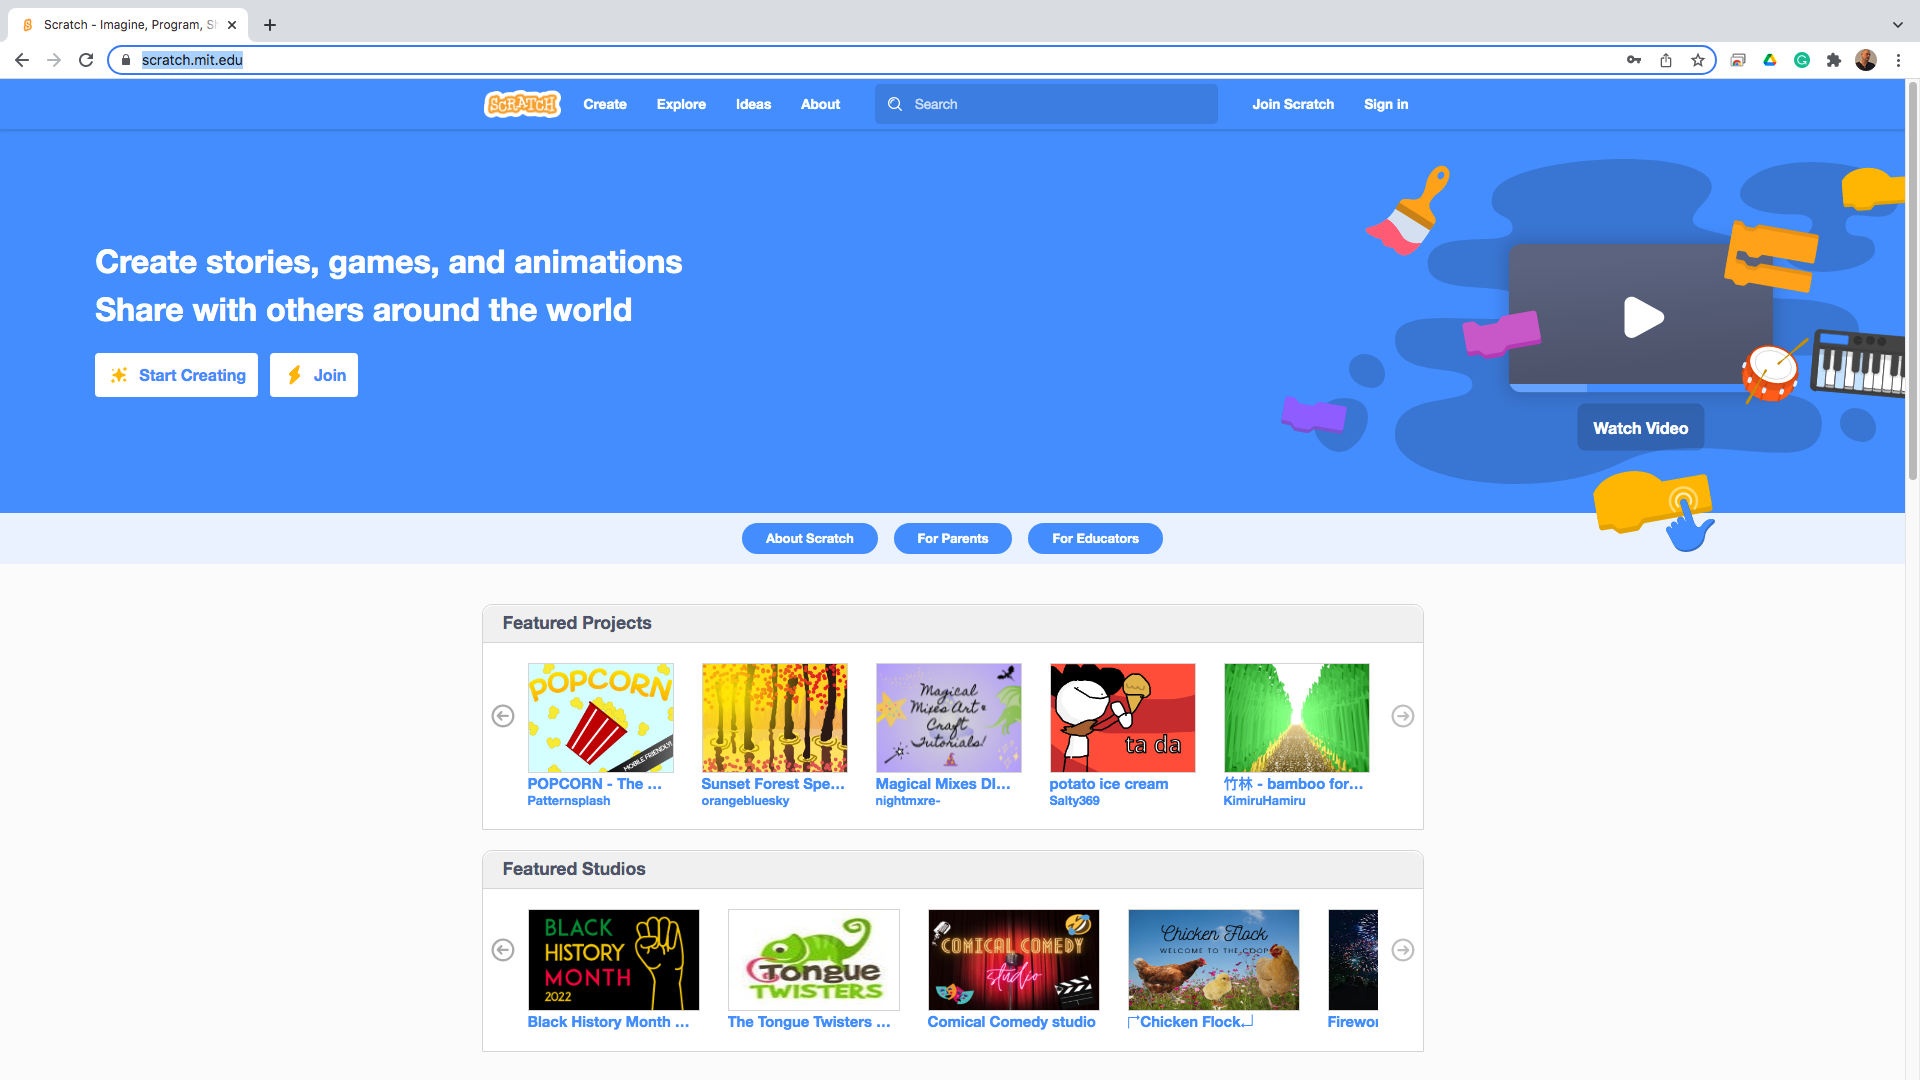
\includegraphics[width=1.0\linewidth,height=0.5\linewidth]{fig010001.png}
  \caption{Начална уеб страница на Scratch}
\label{fig010001}
\end{figure}

Програмната среда на Scratch е организирана на принципа на облачните услуги. Поради тази причина, всеки желаещ да използва услугата трябва да си направи регистрация (Фиг. \ref{fig010002}). Регистрацията се състои от потребителско име и парола.

\begin{figure}[H]
  \centering
  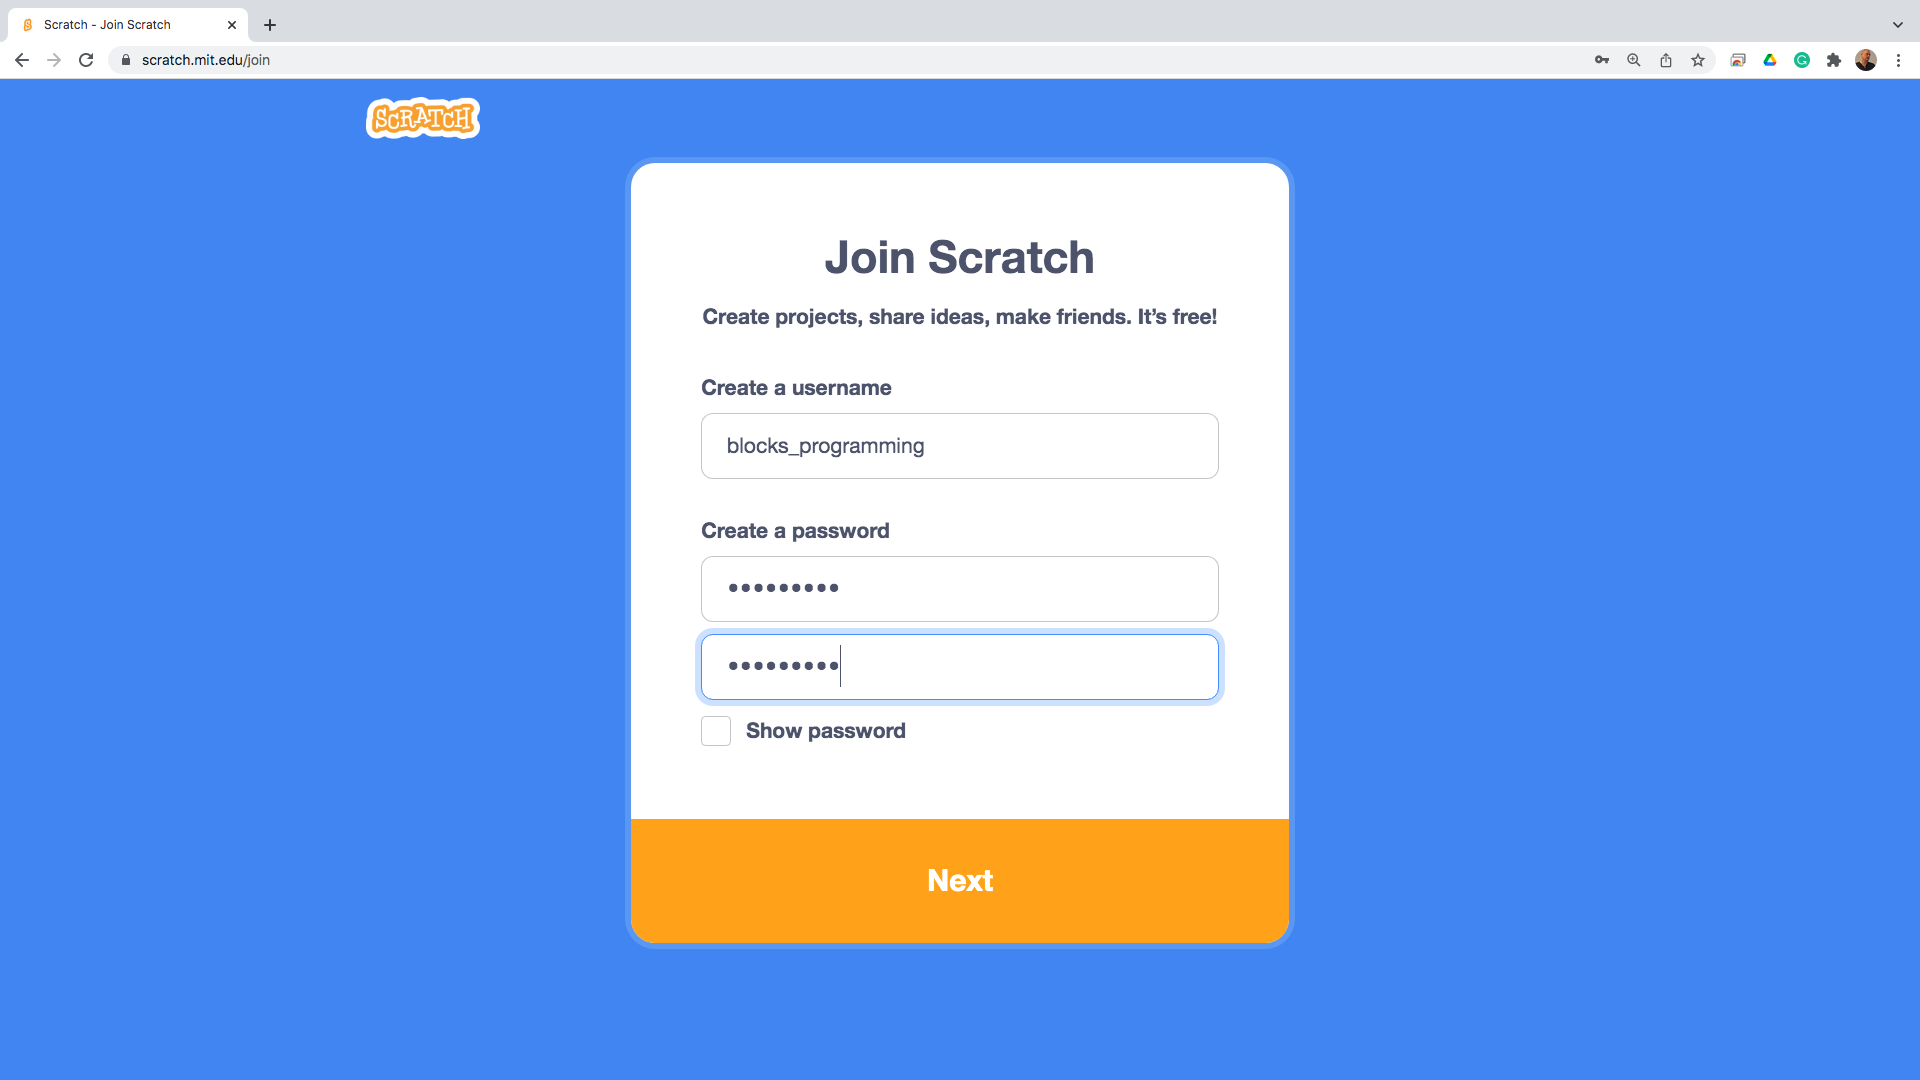
\includegraphics[width=1.0\linewidth,height=0.5\linewidth]{fig010002.png}
  \caption{Регистрация на потребител в Scratch}
\label{fig010002}
\end{figure}

След избора на потребителско име и парола следва определяне на географския регион в който се намира потребителят (Фиг. \ref{fig010003}).

\begin{figure}[H]
  \centering
  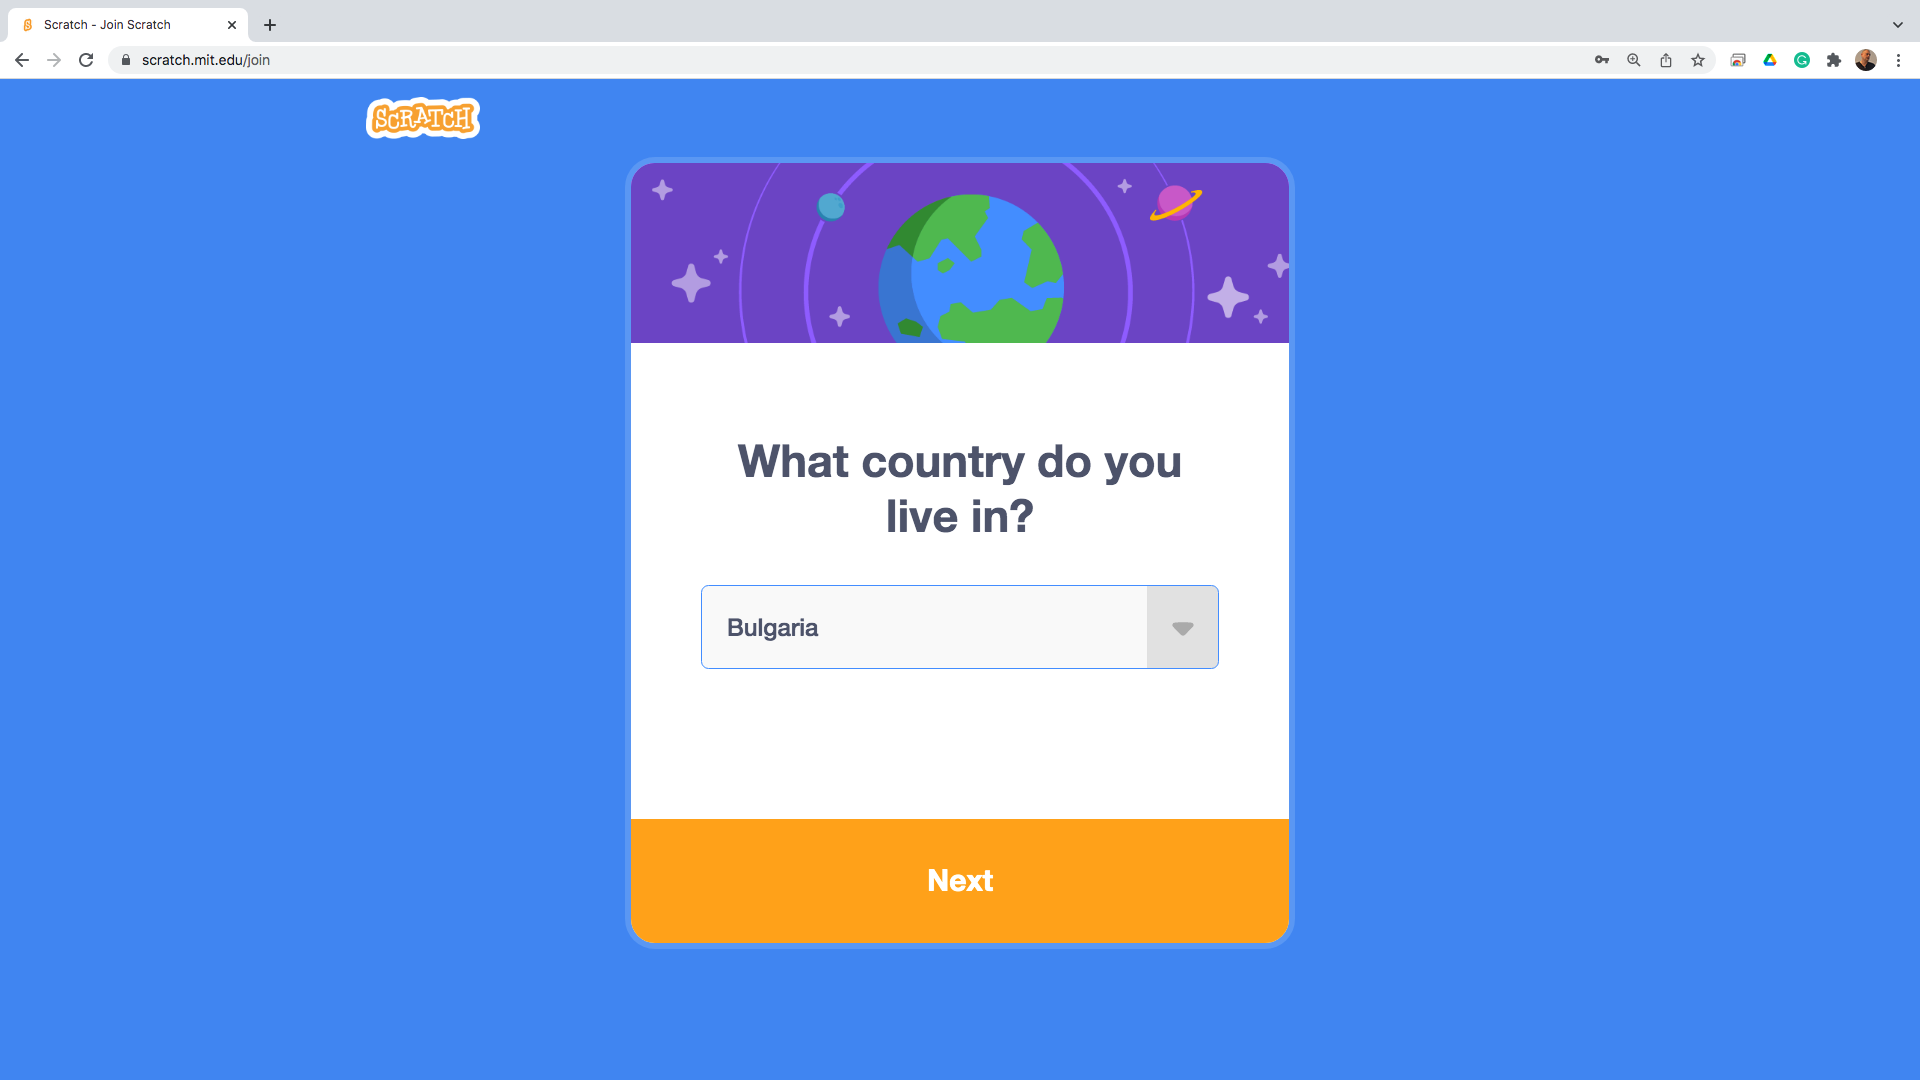
\includegraphics[width=1.0\linewidth,height=0.5\linewidth]{fig010003.png}
  \caption{Географско местоположение}
\label{fig010003}
\end{figure}

Платформата е насочена предимно към деца, изразяващи интерес към програмирането, но също така към родители и учители. Поради тази причина, системата събира информация за възрастта на потребителя (Фиг. \ref{fig010004}).

\begin{figure}[H]
  \centering
  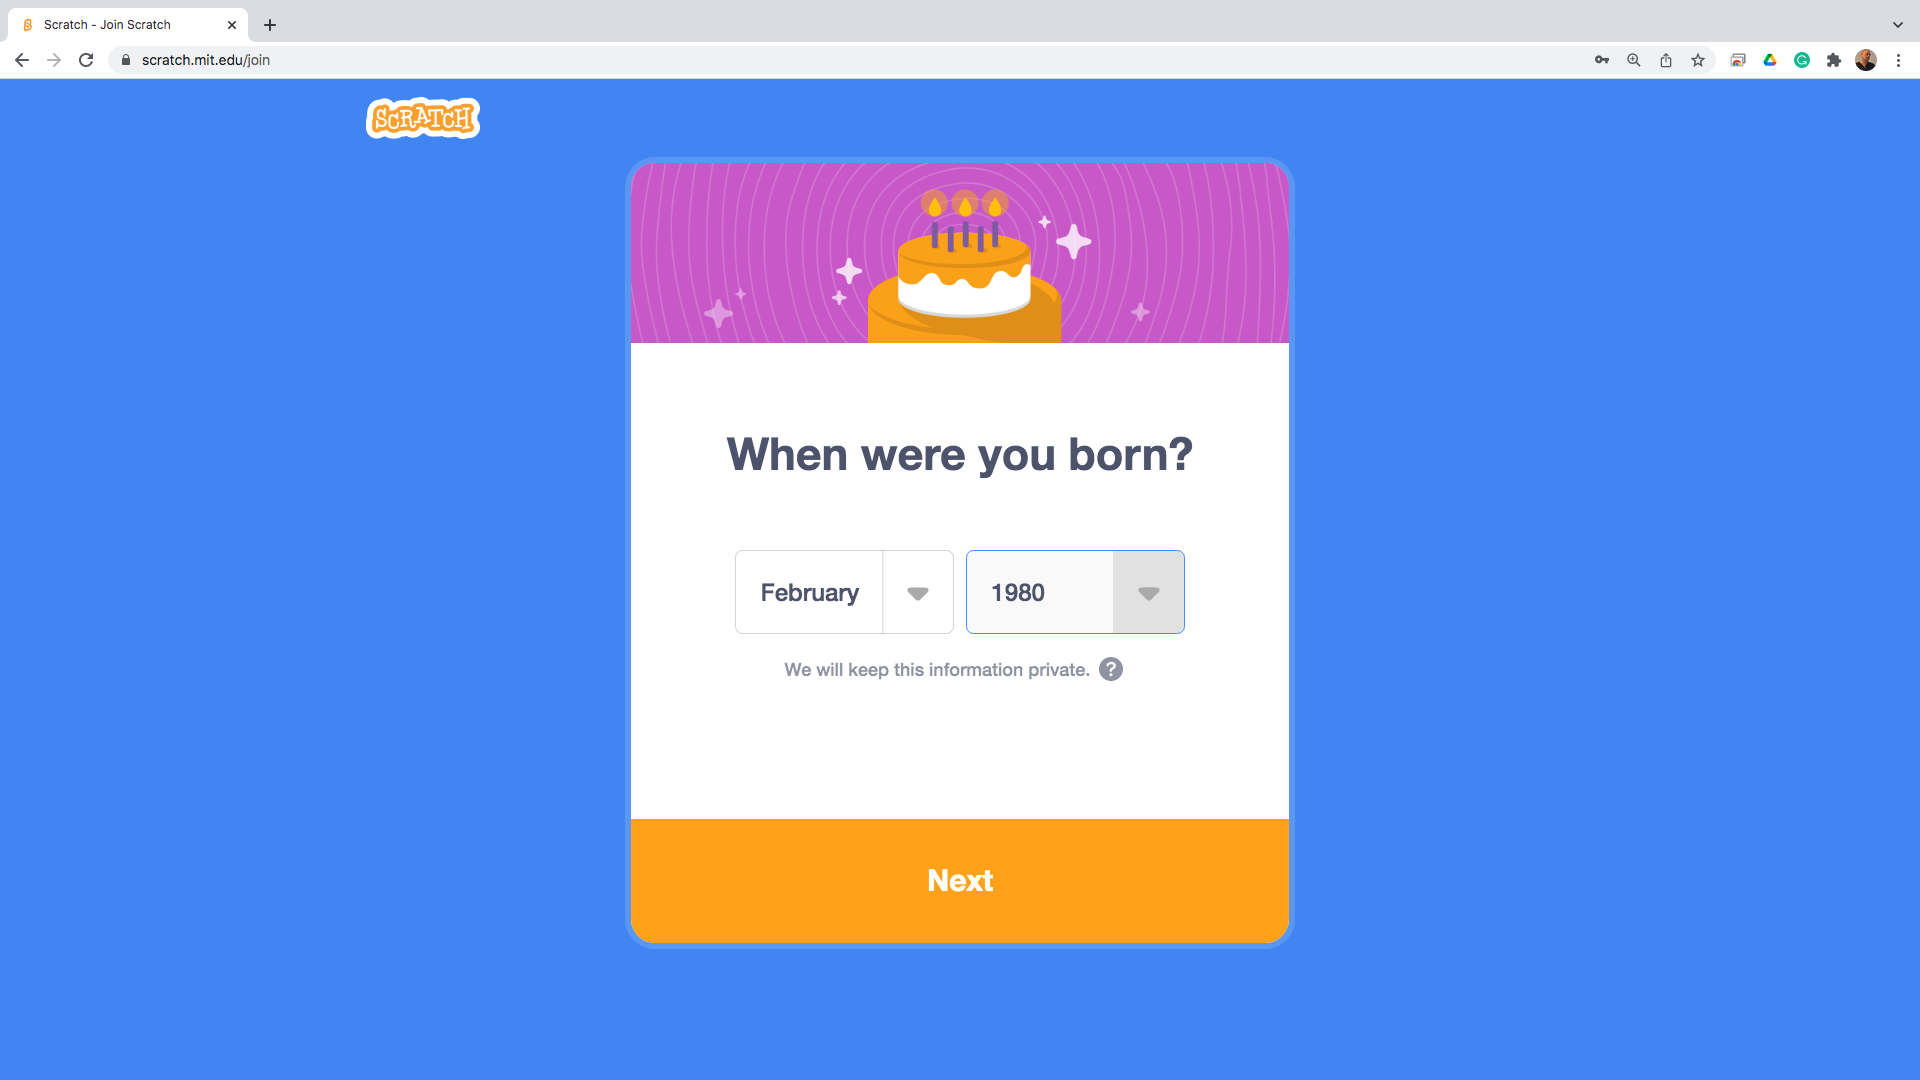
\includegraphics[width=1.0\linewidth,height=0.5\linewidth]{fig010004.png}
  \caption{Възраст на потребителя}
\label{fig010004}
\end{figure}

Освен класификация по възраст, системата събира информация и за класификация по полова принадлежност. Тази информация е незадължителна, основно за да не бъде дискриминираща (Фиг. \ref{fig010005}).

\begin{figure}[H]
  \centering
  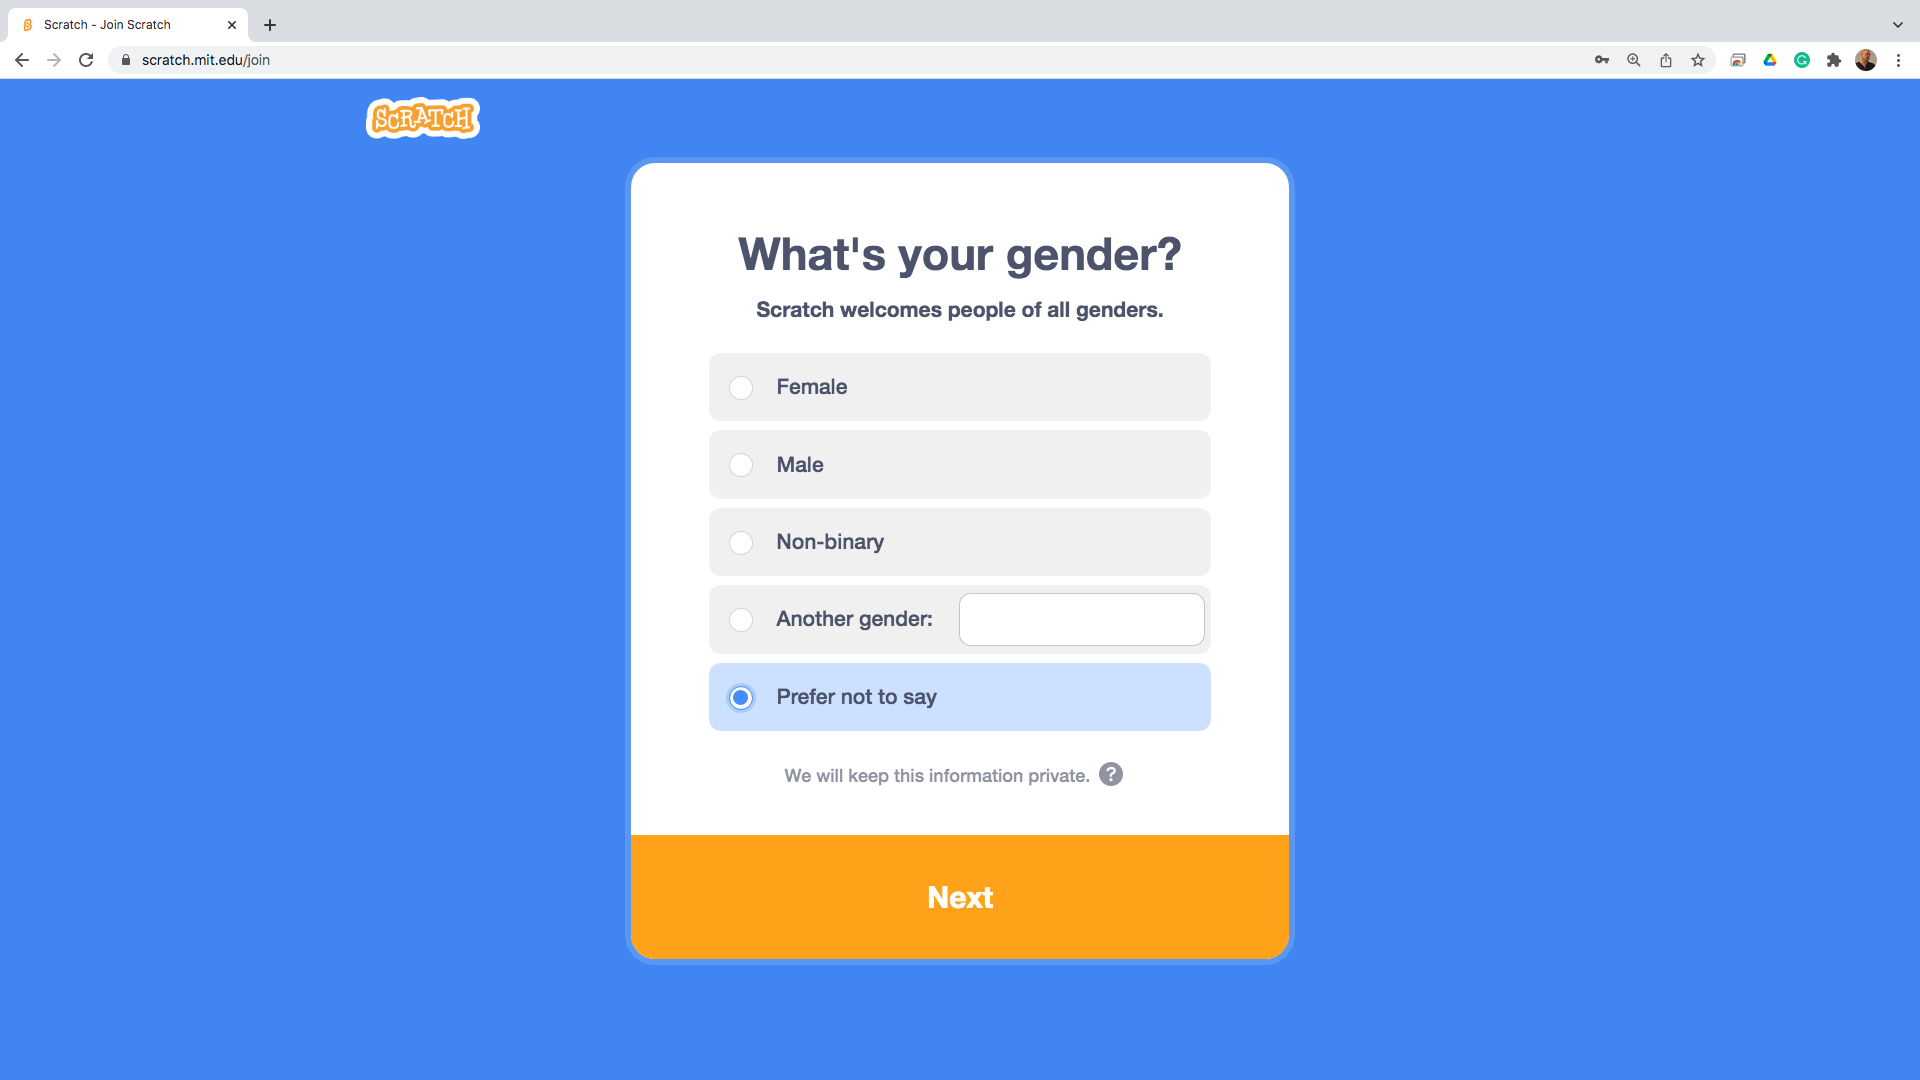
\includegraphics[width=1.0\linewidth,height=0.5\linewidth]{fig010005.png}
  \caption{Пол на потребителя}
\label{fig010005}
\end{figure}

Потребителският профил, освен с потребителско име и парола, трябва да бъде асоцииран и с адрес на електронна пощенска кутия (Фиг. \ref{fig010006}).

\begin{figure}[H]
  \centering
  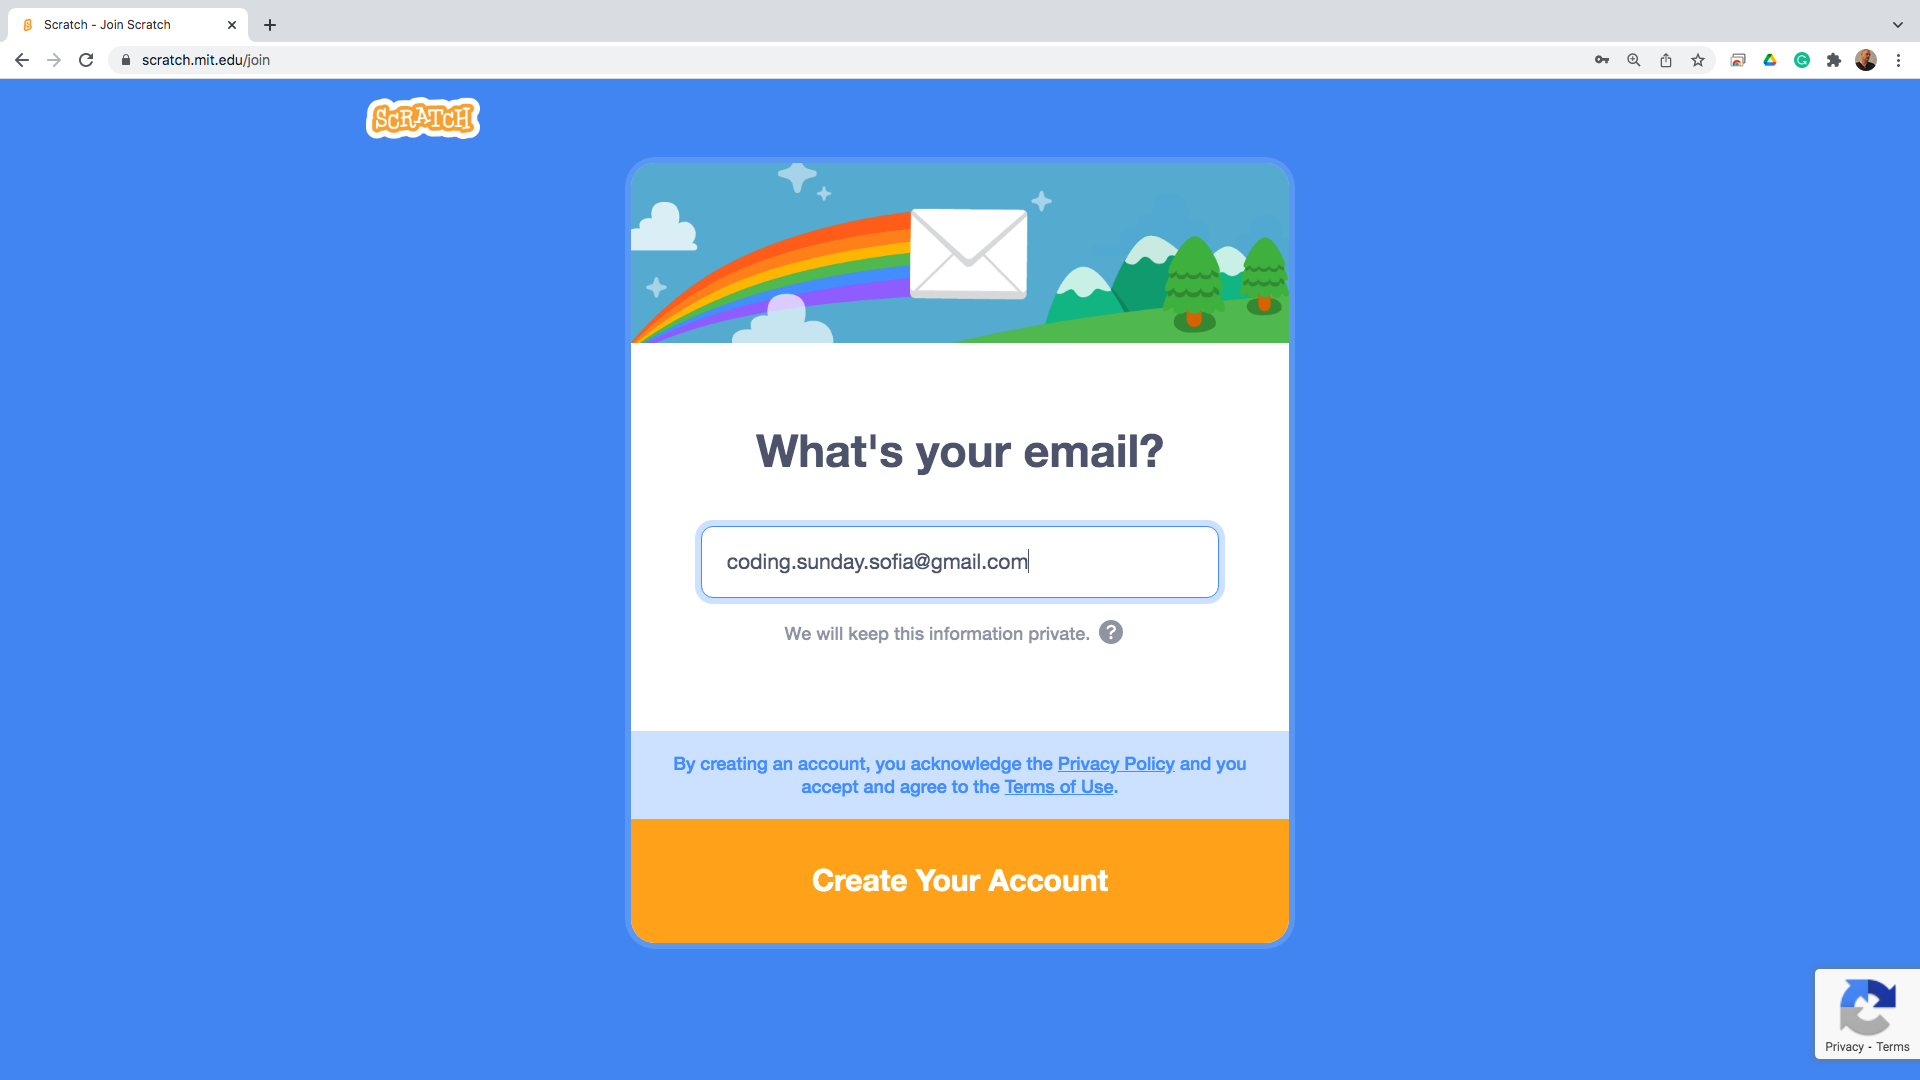
\includegraphics[width=1.0\linewidth,height=0.5\linewidth]{fig010006.png}
  \caption{Адрес на електронна поща на потребителя}
\label{fig010006}
\end{figure}

Процесът по регистрация на потребител в системата е почти завършен (Фиг. \ref{fig010007}). Остава само стъпката за потвърждаване на избрания адрес за електронна поща.

\begin{figure}[H]
  \centering
  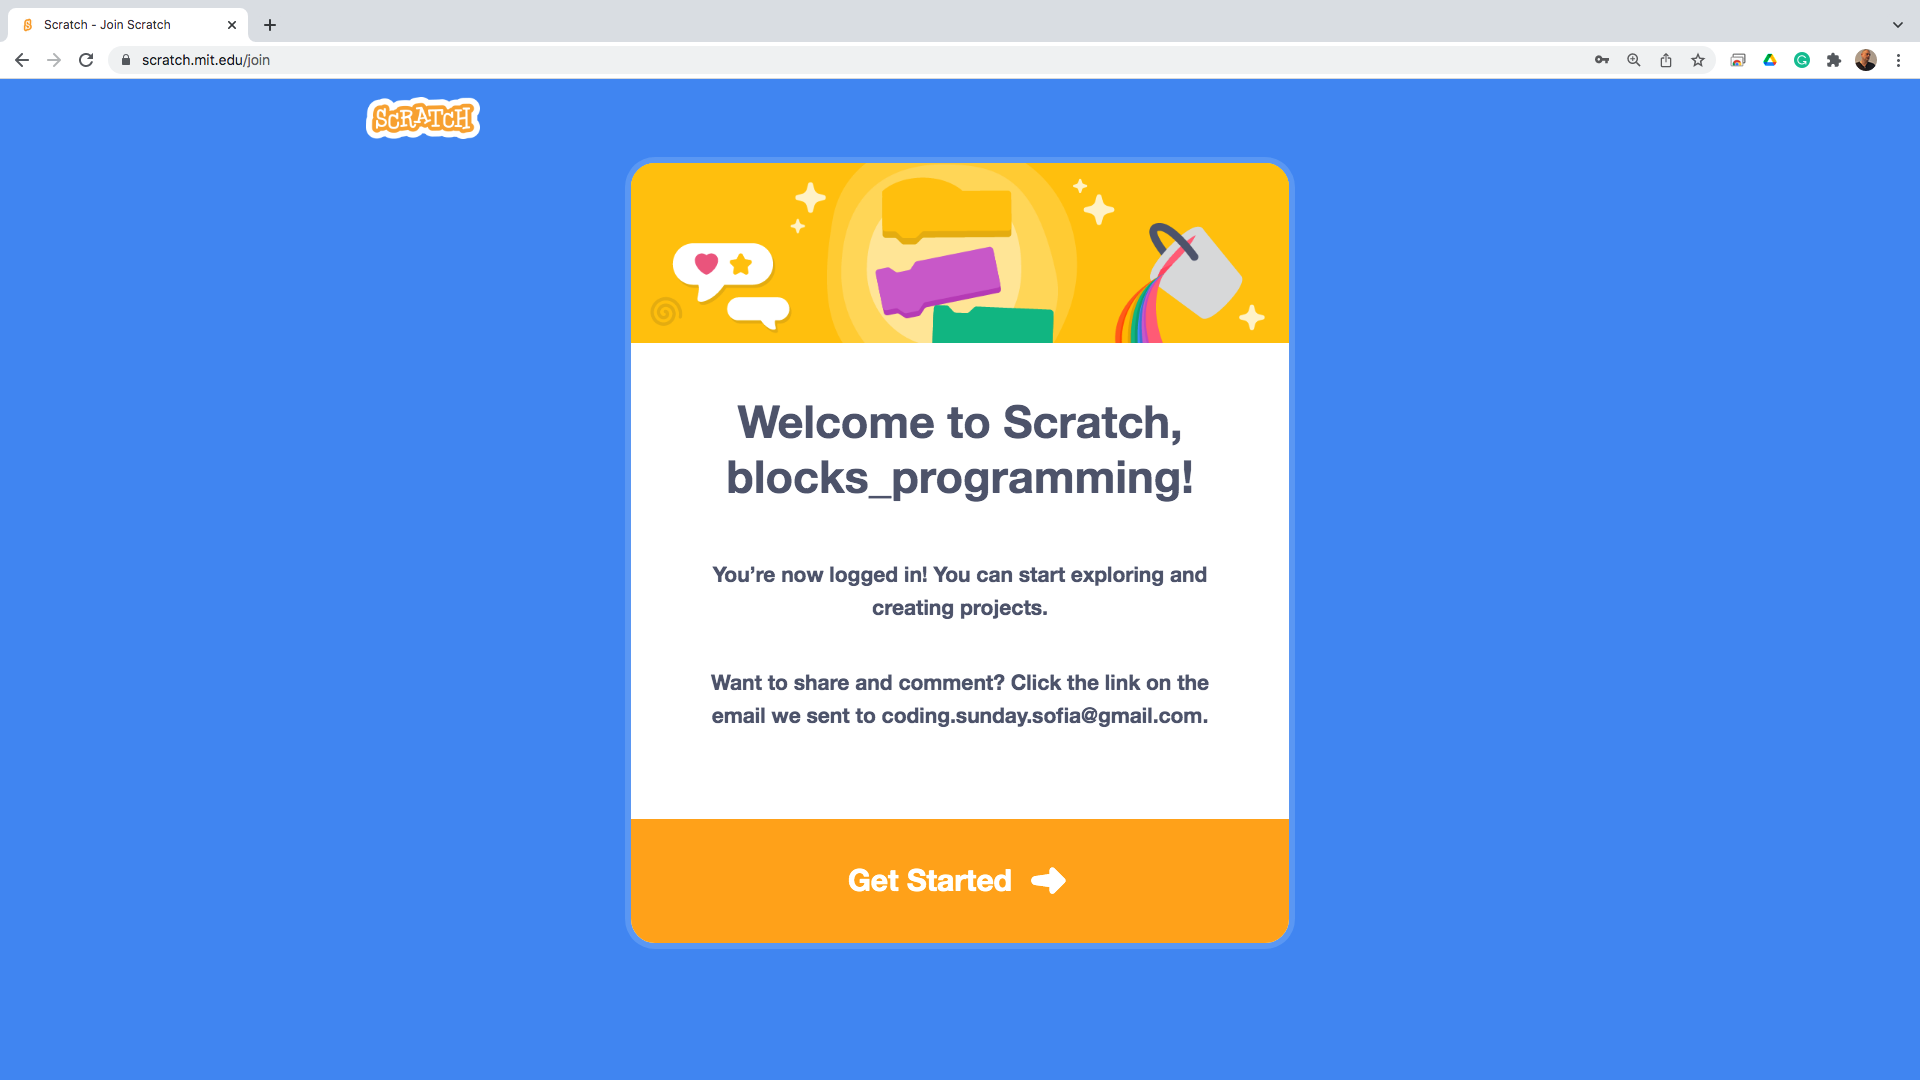
\includegraphics[width=1.0\linewidth,height=0.5\linewidth]{fig010007.png}
  \caption{Приключване на процеса за въвеждане на информация за потребителя}
\label{fig010007}
\end{figure}

Електронното писмо, за потвърждаване на потребителската регистрация, съдържа електронна препратка до уеб сайта на Scratch (Фиг. \ref{fig010008}). Тази препратка трябва да бъде последвана за да се завърши процесът по регистрация на нов потребител. 

\begin{figure}[H]
  \centering
  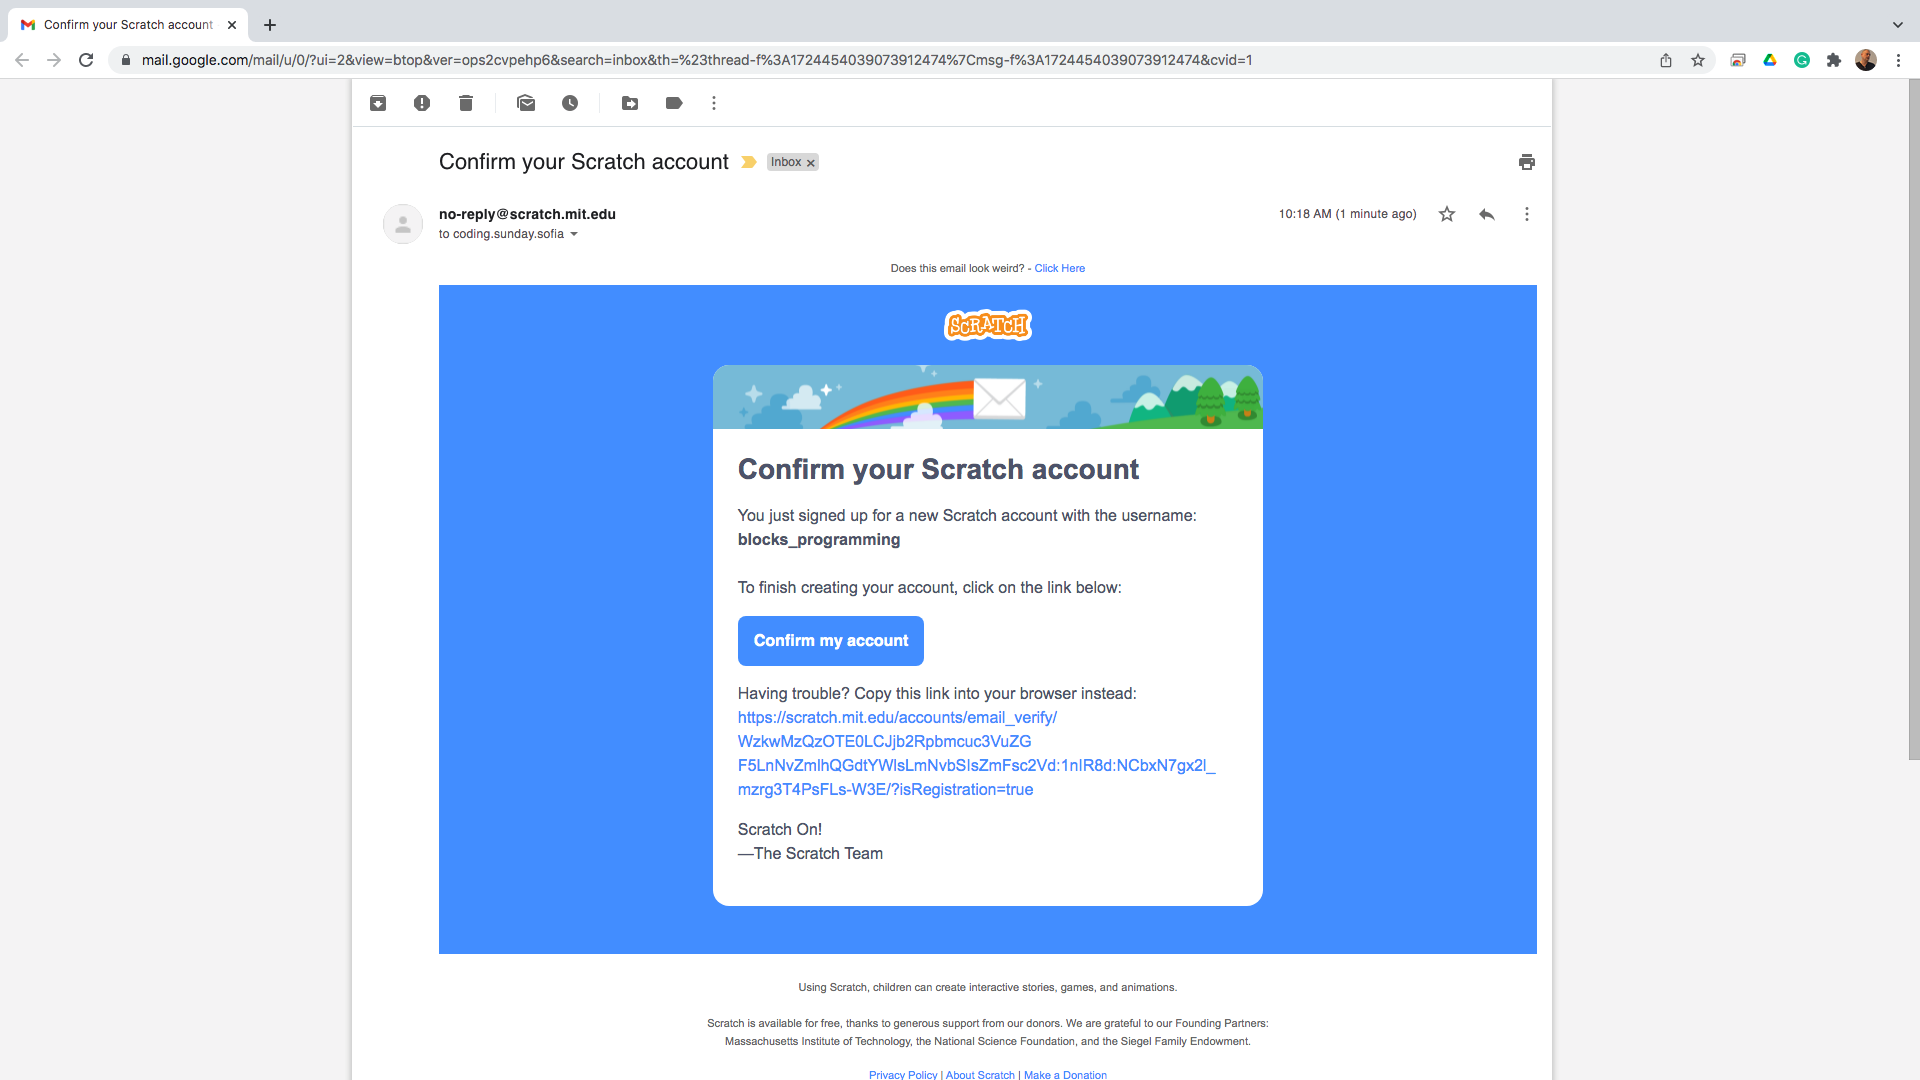
\includegraphics[width=1.0\linewidth,height=0.5\linewidth]{fig010008.png}
  \caption{Електронно съобщение за потвърждаване на електронния адрес}
\label{fig010008}
\end{figure}

Регистрацията на новия потребител приключва със зареждането на начален работен екран (Фиг. \ref{fig010009}). Горе, в дясно се вижда изписано потребителското име, избрано на първата стъпка от процеса по регистрацията.

\begin{figure}[H]
  \centering
  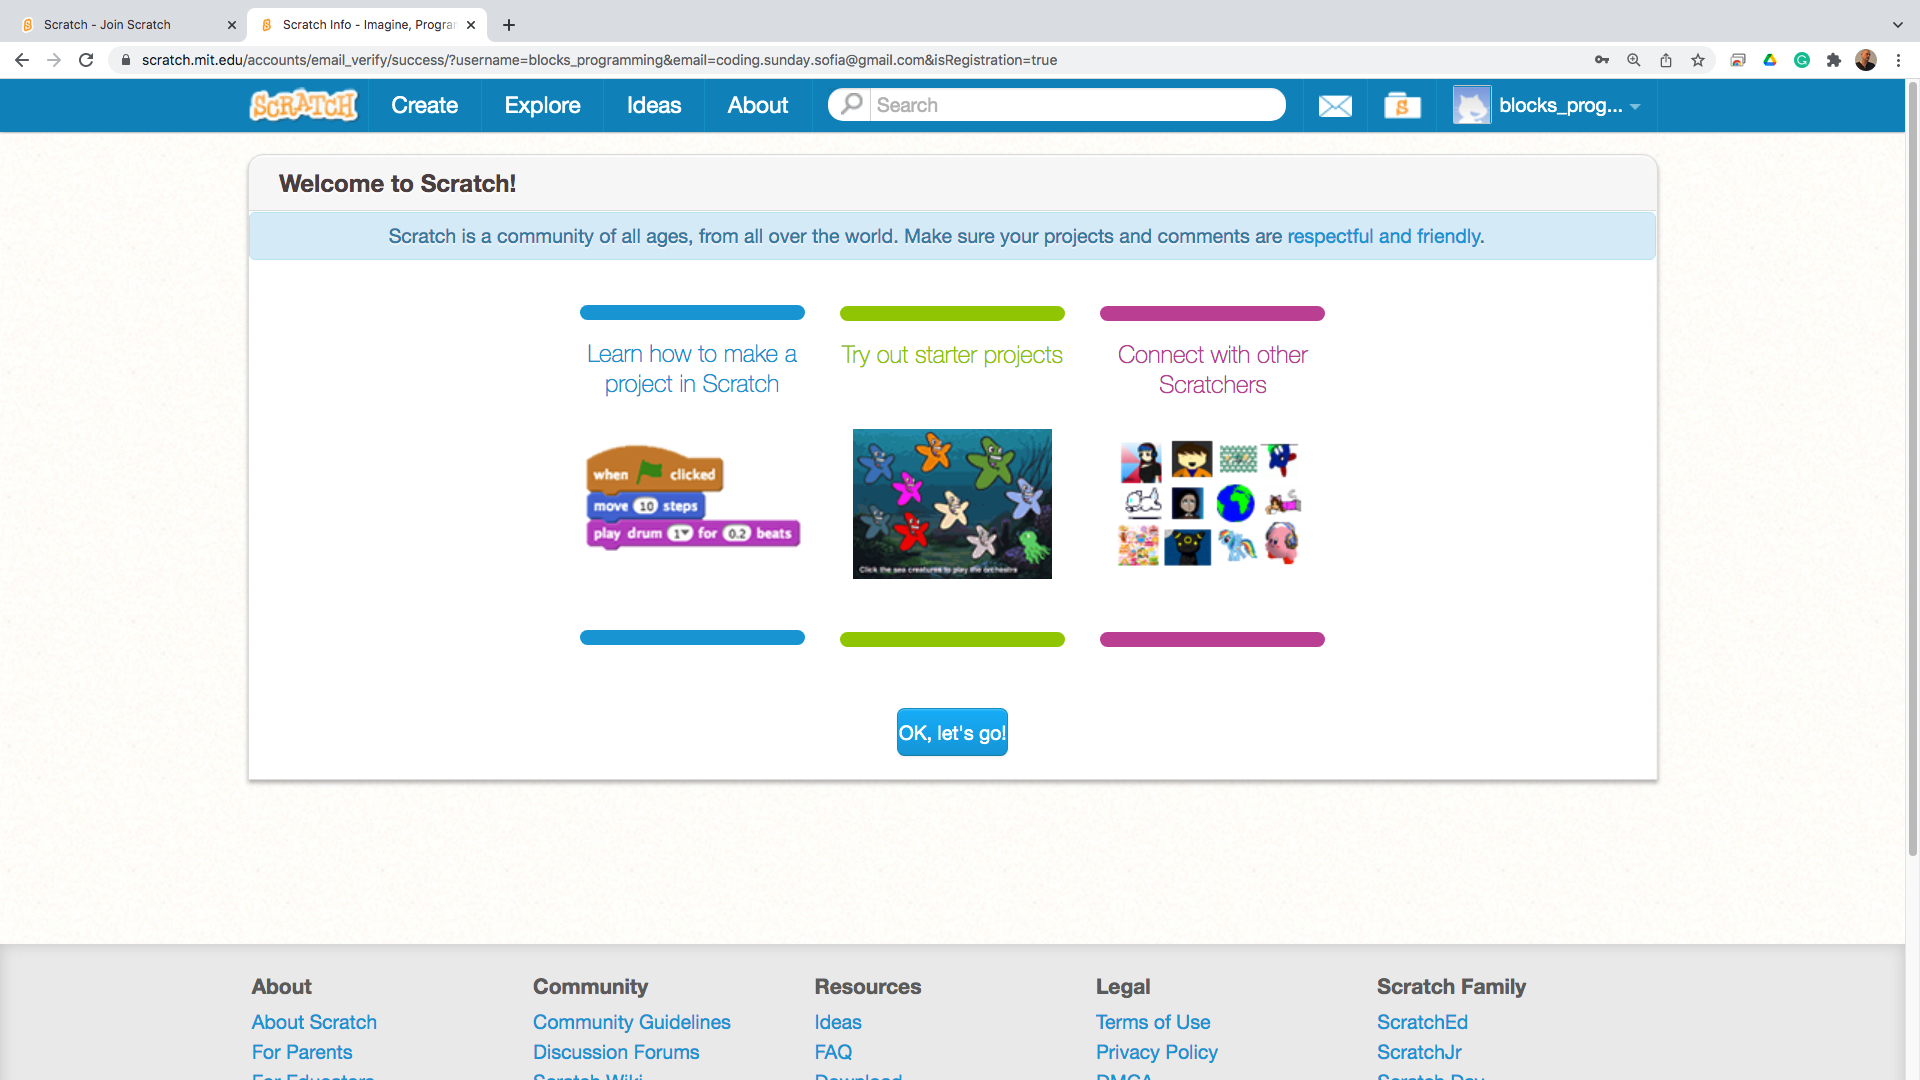
\includegraphics[width=1.0\linewidth,height=0.5\linewidth]{fig010009.png}
  \caption{Начален работен екран}
\label{fig010009}
\end{figure}

Успешната регистрация може да се потвърди и чрез създаването на много малък проект, който да демонстрира функционирането на развойната среда. За тази цел се избира опцията „Create“ от менюто (Фиг. \ref{fig010010}).

\begin{figure}[H]
  \centering
  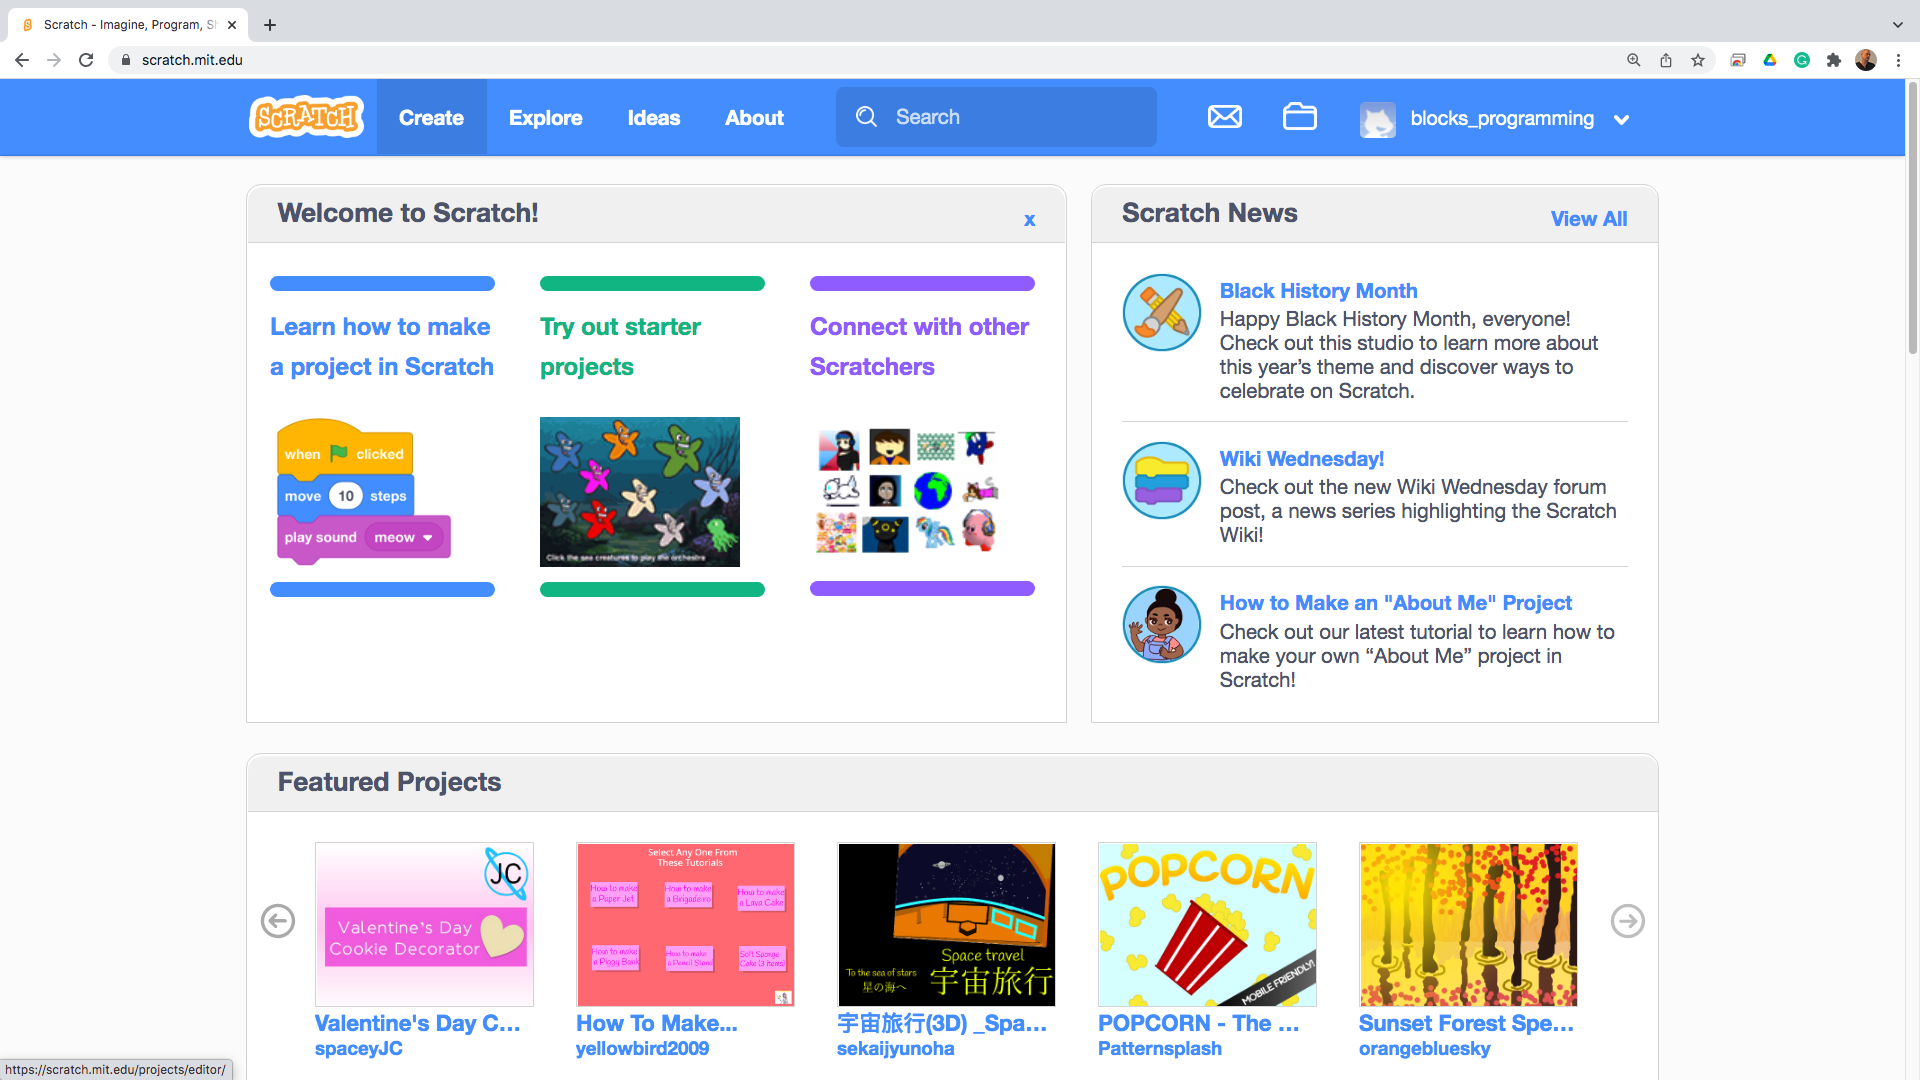
\includegraphics[width=1.0\linewidth,height=0.5\linewidth]{fig010010.png}
  \caption{Избор на опция от менюто за нов проект}
\label{fig010010}
\end{figure}

Създаването на нов проект преминава през серия стъпки, свързани със заделянето на първоначално нужните ресурси (Фиг. \ref{fig010011}).

\begin{figure}[H]
  \centering
  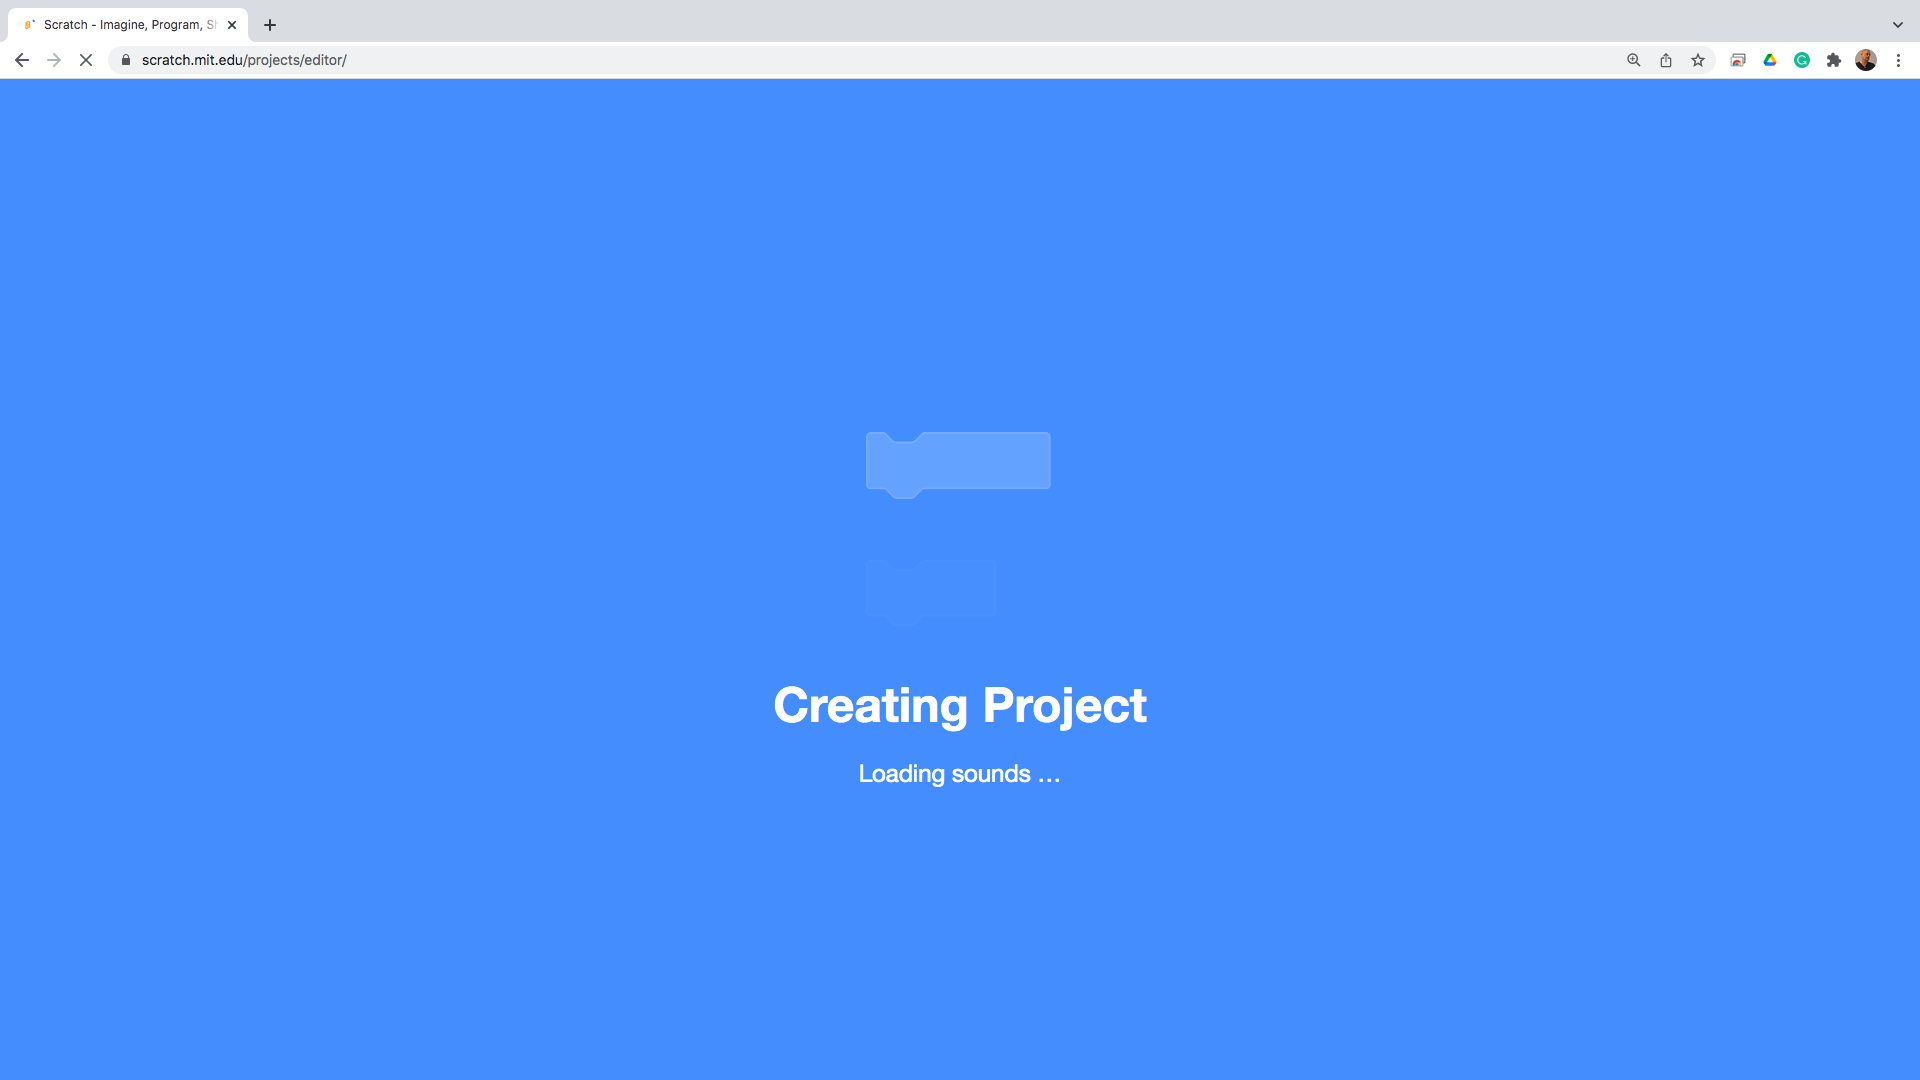
\includegraphics[width=1.0\linewidth,height=0.5\linewidth]{fig010011.png}
  \caption{Зареждане на ресурсите}
\label{fig010011}
\end{figure}

След зареждането на новия проект се визуализира работното пространство (Фиг. \ref{fig010012}). Най- в ляво е списъкът с възможни програмни инструкции, под формата на парченца от пъзел. В централната част е работното пространство, където инструкциите се подреждат. А най- в дясно е активната сцена, където се визуализират действията, заложени в серията от инструкции. 

\begin{figure}[H]
  \centering
  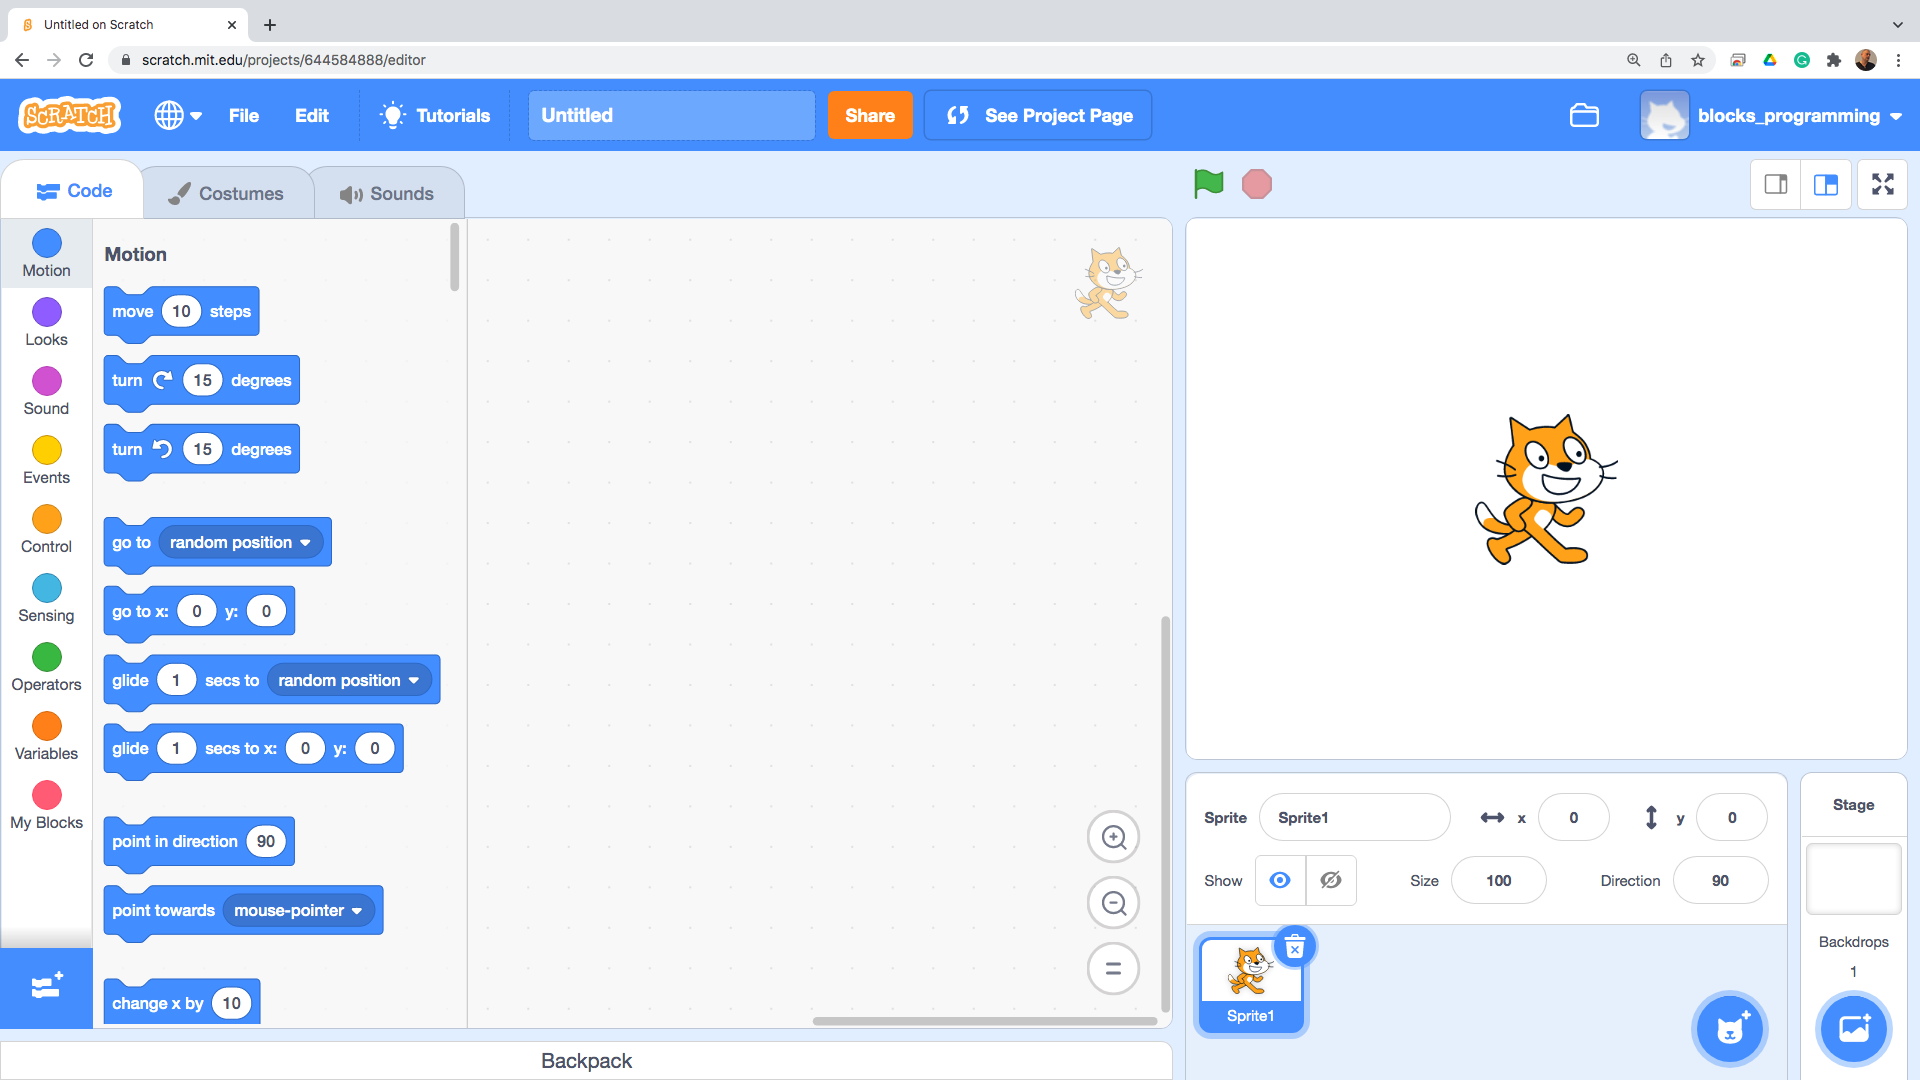
\includegraphics[width=1.0\linewidth,height=0.5\linewidth]{fig010012.png}
  \caption{Организация на работното пространство}
\label{fig010012}
\end{figure}

Всяка компютърна програма има своя начална точка и своя крайна точка. В Scratch, за началото на програмата има специално отделен блок (програмна инструкция), която е показна на Фиг. \ref{fig010013}. Изпълнението на програмите, написани в Scratch, започва с натискането на зеления флаг. Точно поради тази причина, блокчето за старт на програмата е свързано със събитието за натискане на зеления флаг. 

\begin{figure}[H]
  \centering
  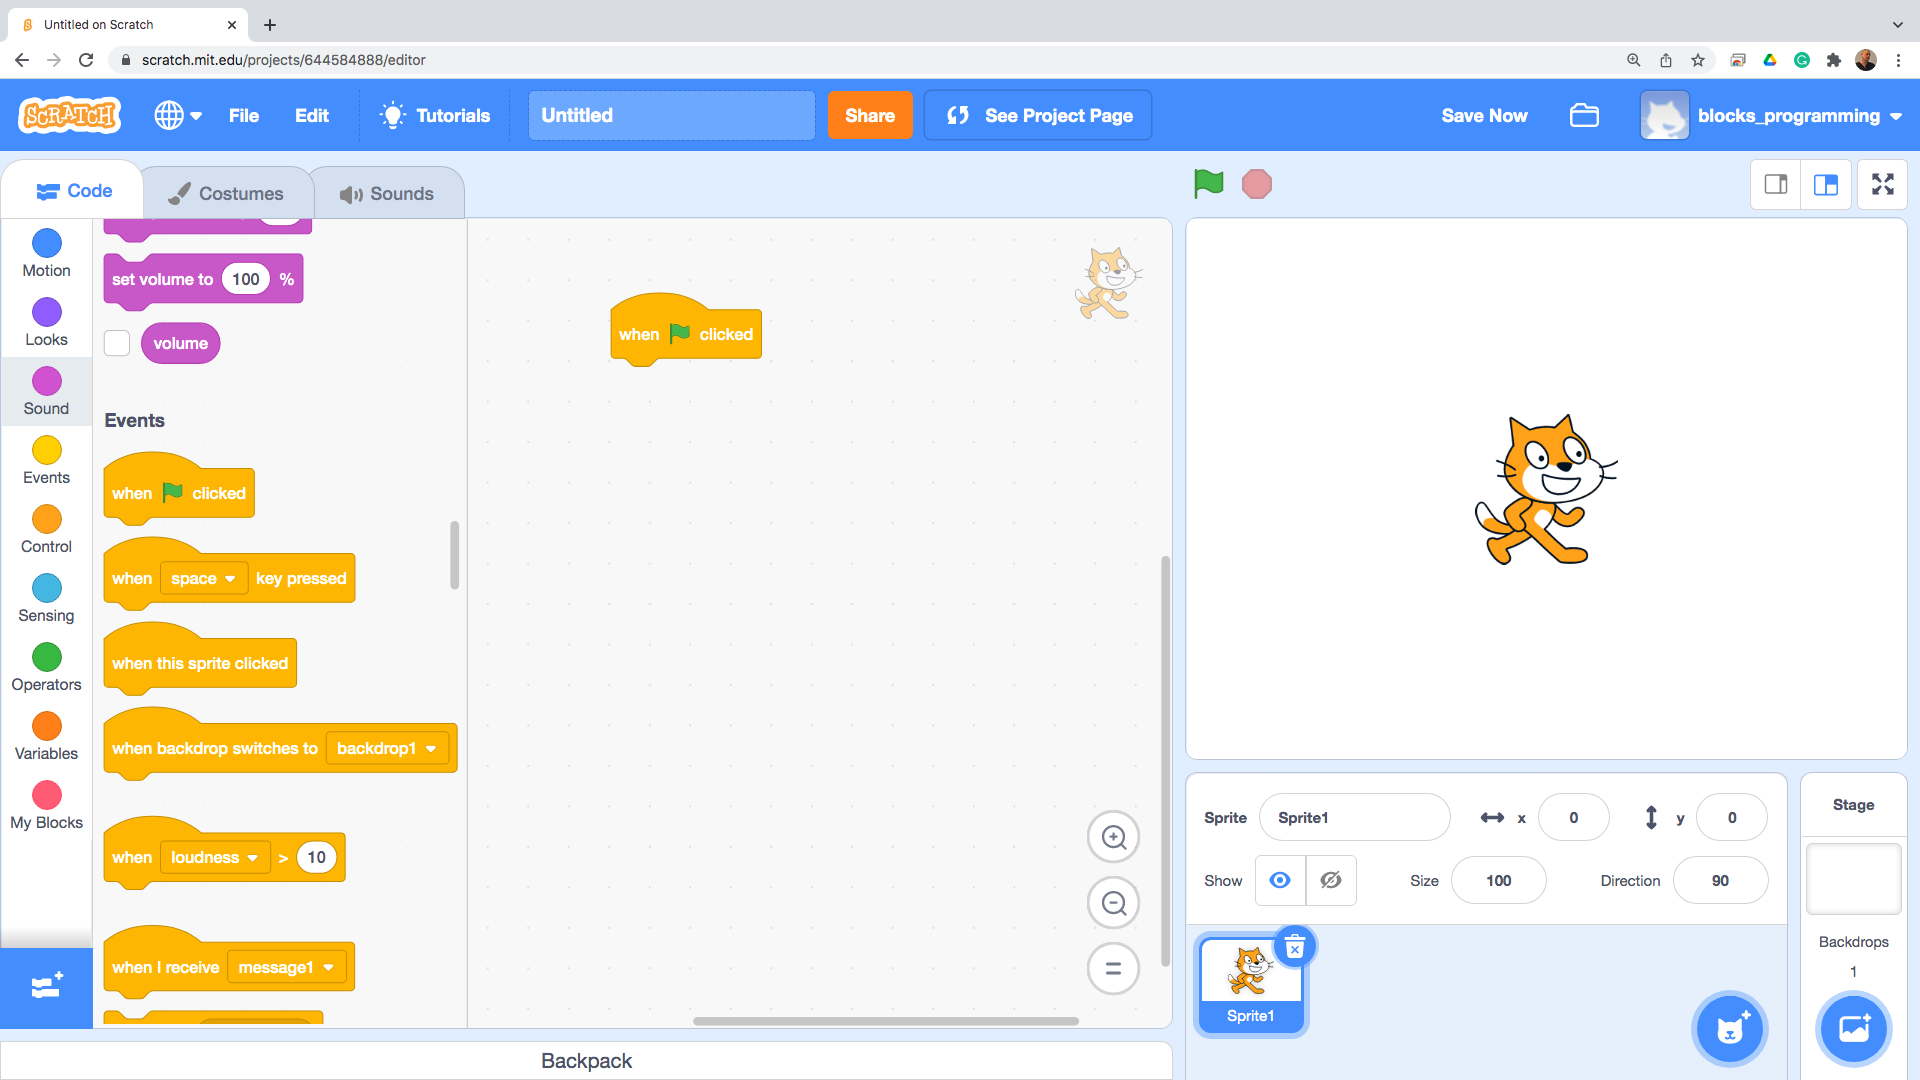
\includegraphics[width=1.0\linewidth,height=0.5\linewidth]{fig010013.png}
  \caption{Начало на програмата}
\label{fig010013}
\end{figure}

Една от най-интуитивните и същевременно лесно разбираеми инструкции е преместване с определен брой стъпки (Фиг. \ref{fig010014}). Главен актьор в началната сцена на Scratch е оранжевият котарак. Ако сцената не бъде променяна, то инструкциите за извършване на различни действия се насочват точно към този котарак. 

\begin{figure}[H]
  \centering
  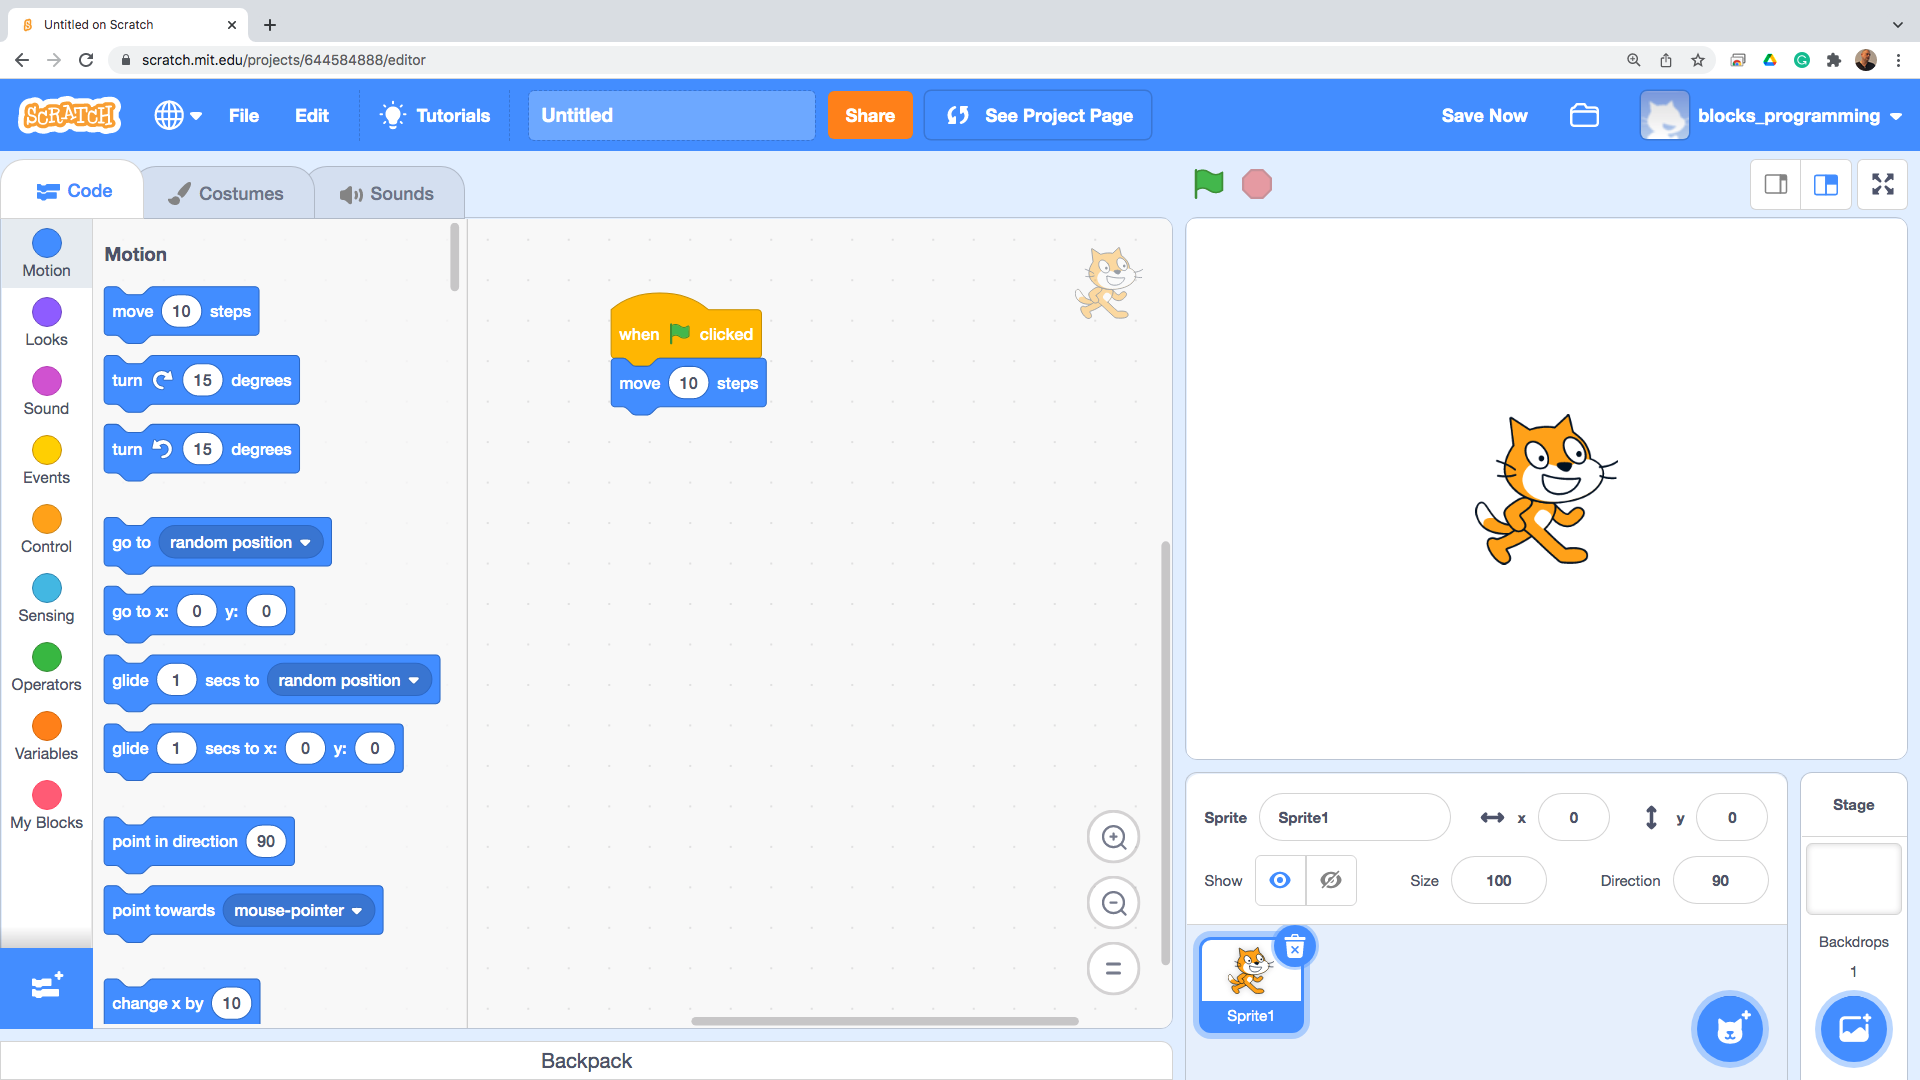
\includegraphics[width=1.0\linewidth,height=0.5\linewidth]{fig010014.png}
  \caption{Инструкция за придвижване на стъпки}
\label{fig010014}
\end{figure}

След преместването на котарака е от съществено значение да има една пауза на изчакване, така че визуално да се забележи преместването. За тази цел може да се приложи инструкция за изчакване, за определен брой секунди (Фиг. \ref{fig010015}).

\begin{figure}[H]
  \centering
  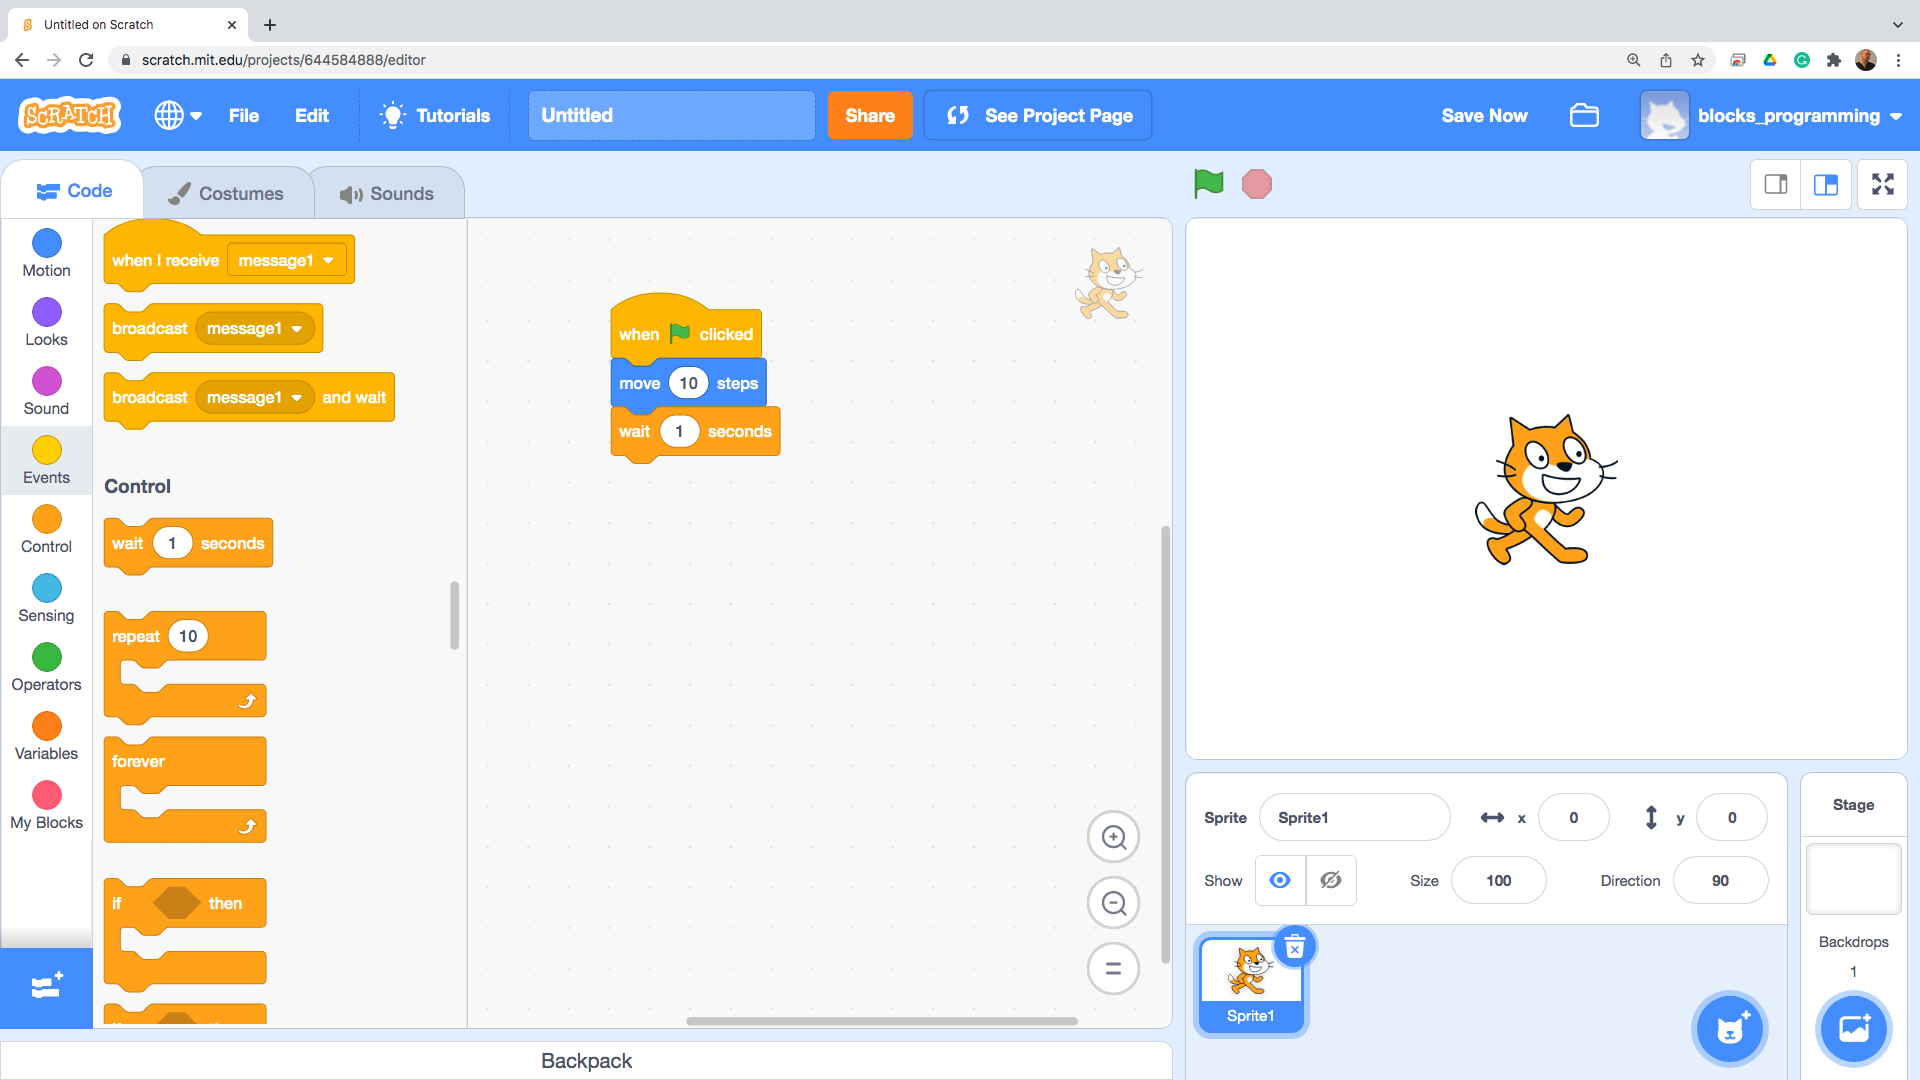
\includegraphics[width=1.0\linewidth,height=0.5\linewidth]{fig010015.png}
  \caption{Инструкция за изчакване}
\label{fig010015}
\end{figure}

След изчакването, котката може да се върне на първоначалната си позиция, като се изпълни инструкция за придвижване с отрицателен брой стъпки (Фиг. \ref{fig010016}).

\begin{figure}[H]
  \centering
  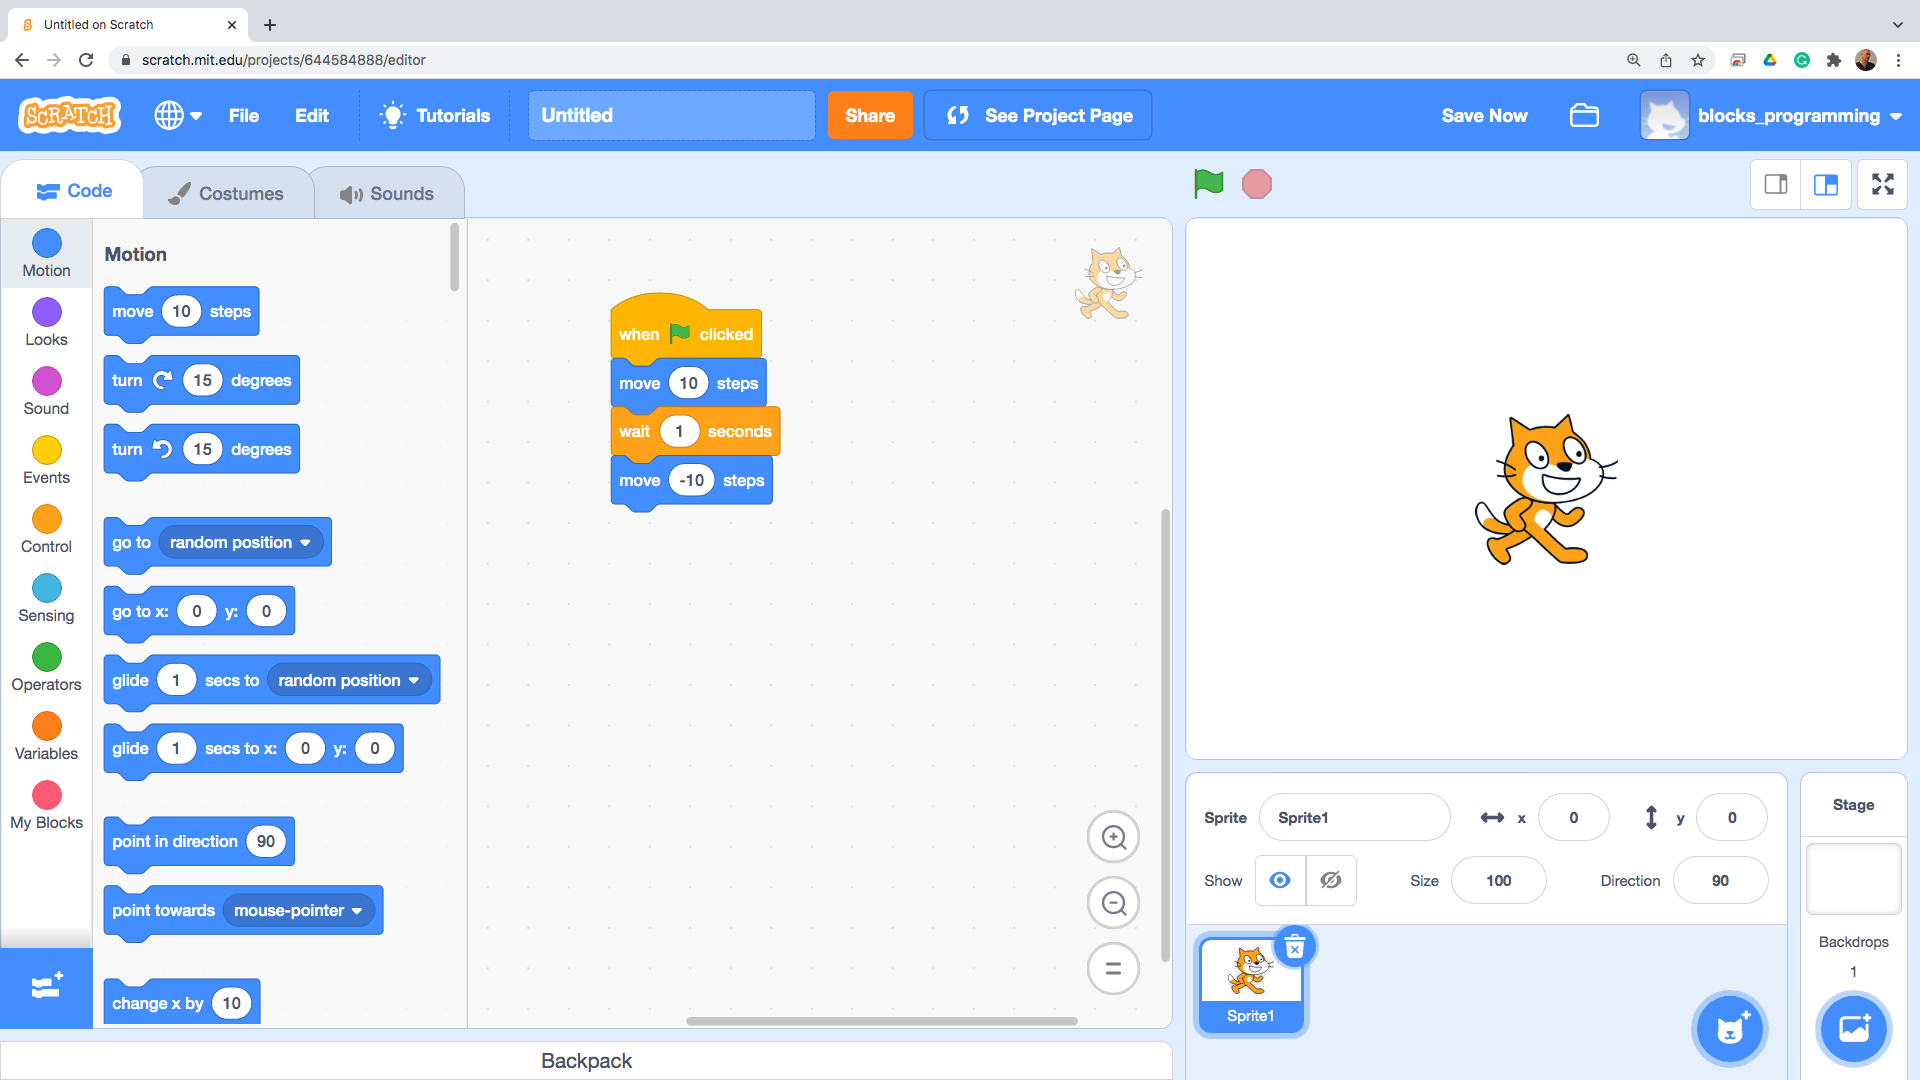
\includegraphics[width=1.0\linewidth,height=0.5\linewidth]{fig010016.png}
  \caption{Инструкция за преместване обратно}
\label{fig010016}
\end{figure}

След като всички предвидени инструкции са изпълнени е разумно да се сложи край на програмата, за което е предвидено отделно блокче в списъка с инструкции (Фиг. \ref{fig010017}).

\begin{figure}[H]
  \centering
  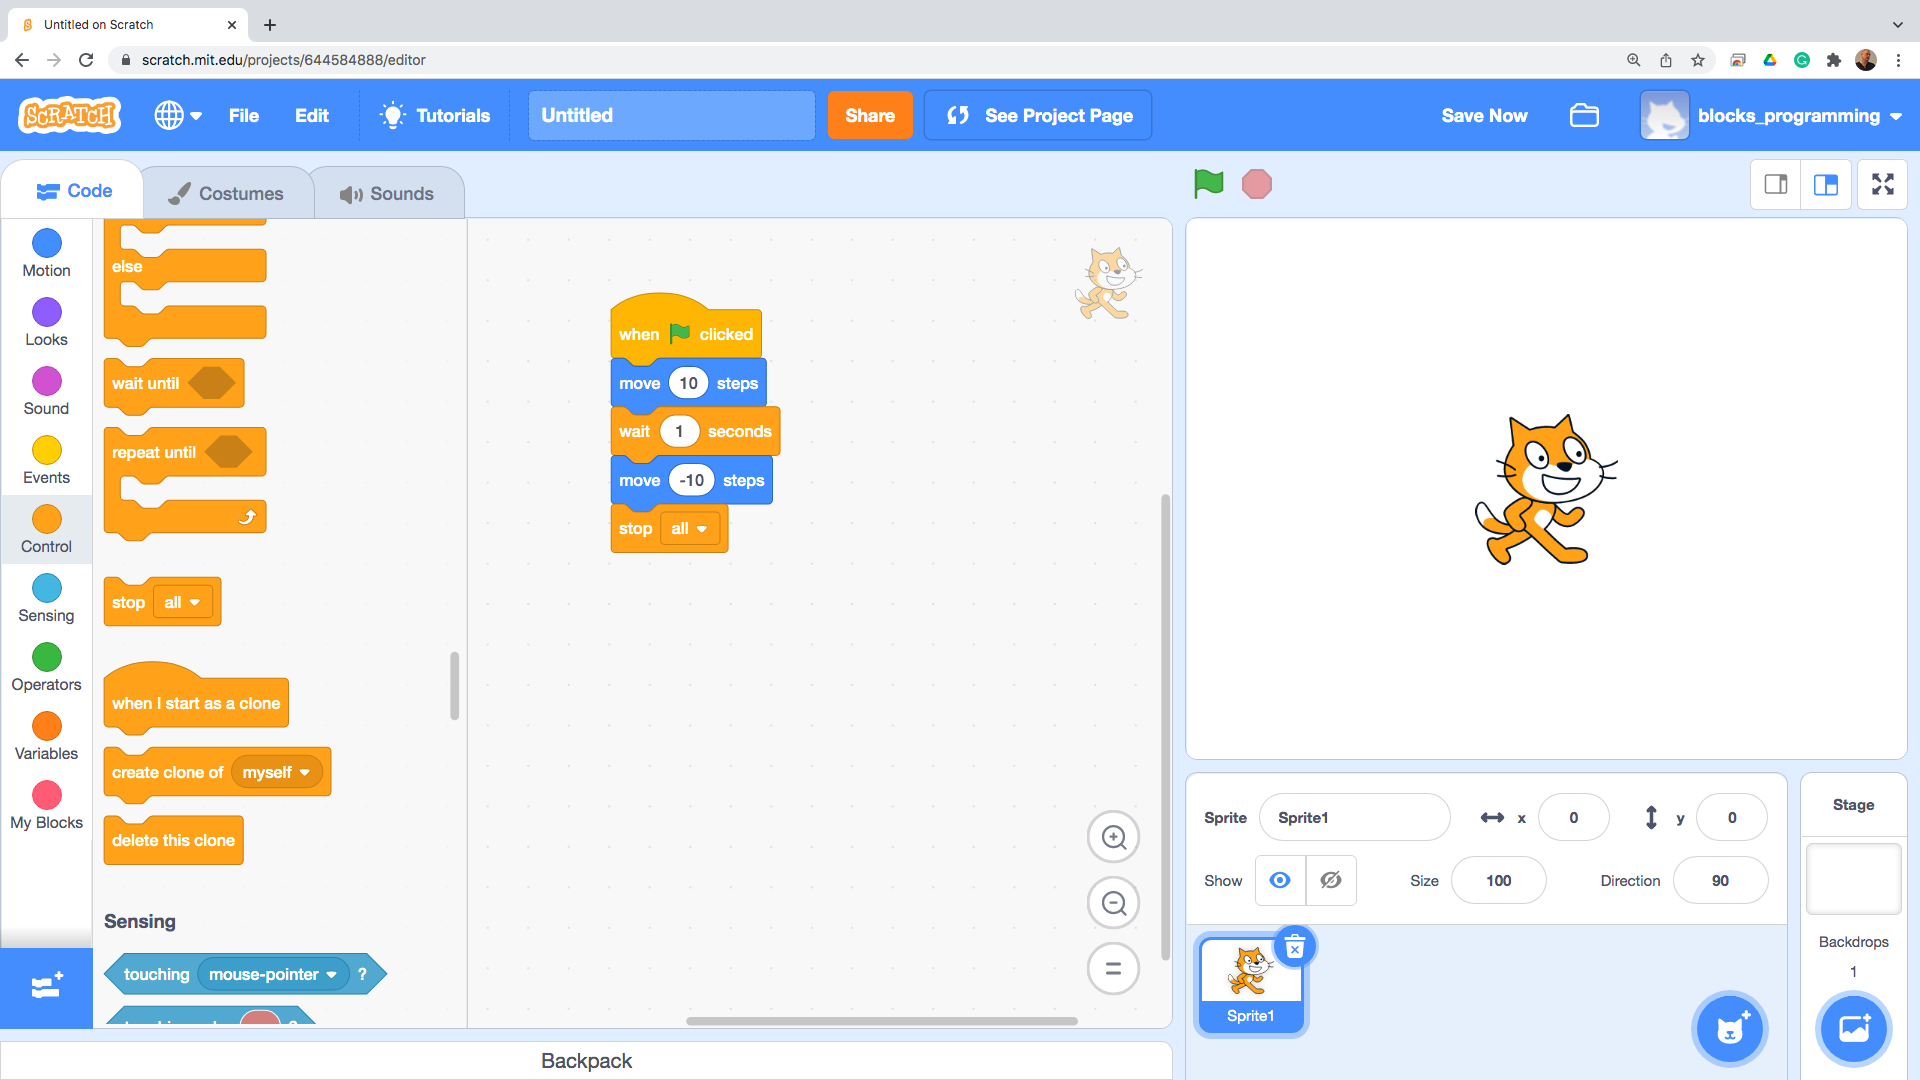
\includegraphics[width=1.0\linewidth,height=0.5\linewidth]{fig010017.png}
  \caption{Инструкция за край}
\label{fig010017}
\end{figure}

Така написаната програма се изпълнява, чрез натискане на зеления флаг (Фиг. \ref{fig010018}), а при нужда от аварийно спиране се натиска червеният кръг, от дясно на зеления флаг.

\begin{figure}[H]
  \centering
  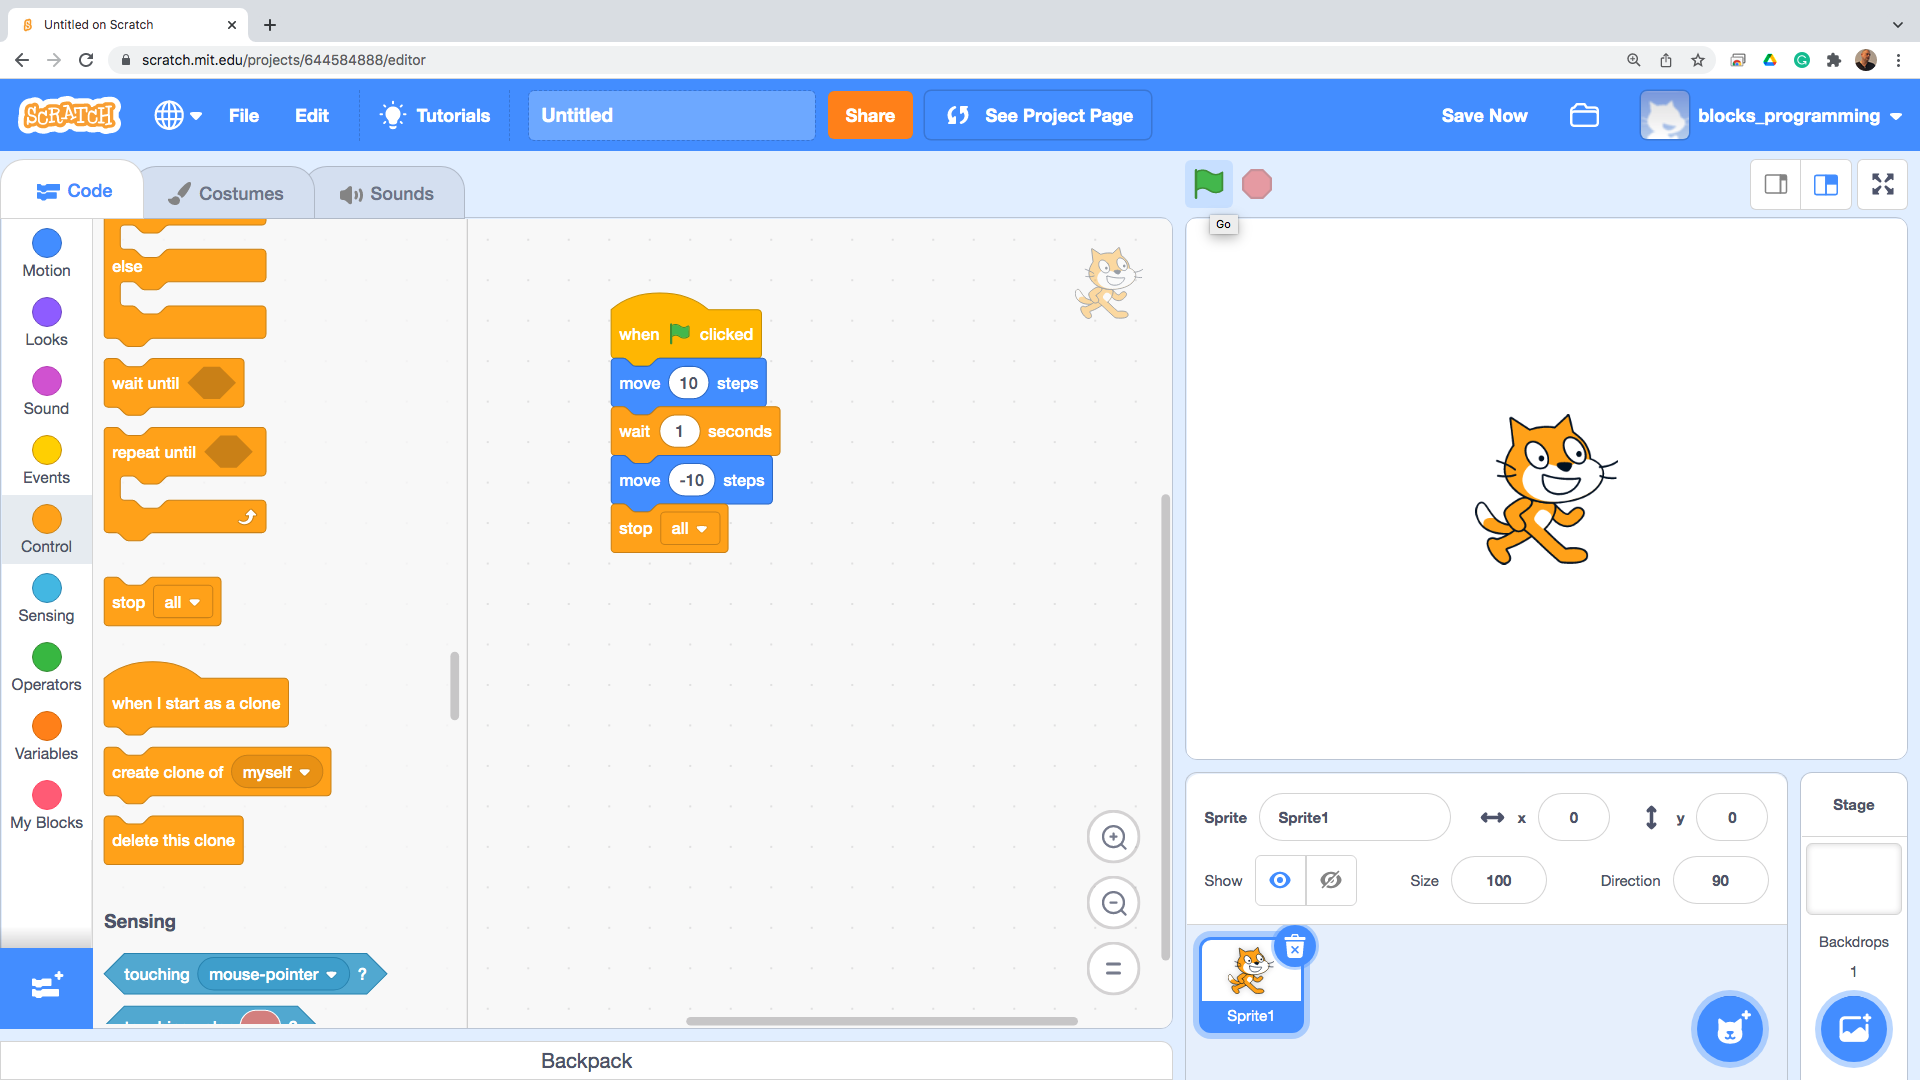
\includegraphics[width=1.0\linewidth,height=0.5\linewidth]{fig010018.png}
  \caption{Изпълнение на програмата}
\label{fig010018}
\end{figure}

Всяка програма, която се пише в Scratch се помества в отделен проект. Достъп до всички проекти на потребителя може да се получи от менюто „My Stuff“, което е част от списъка с опции за боравене с регистрирания потребител (Фиг. \ref{fig010019}).

\begin{figure}[H]
  \centering
  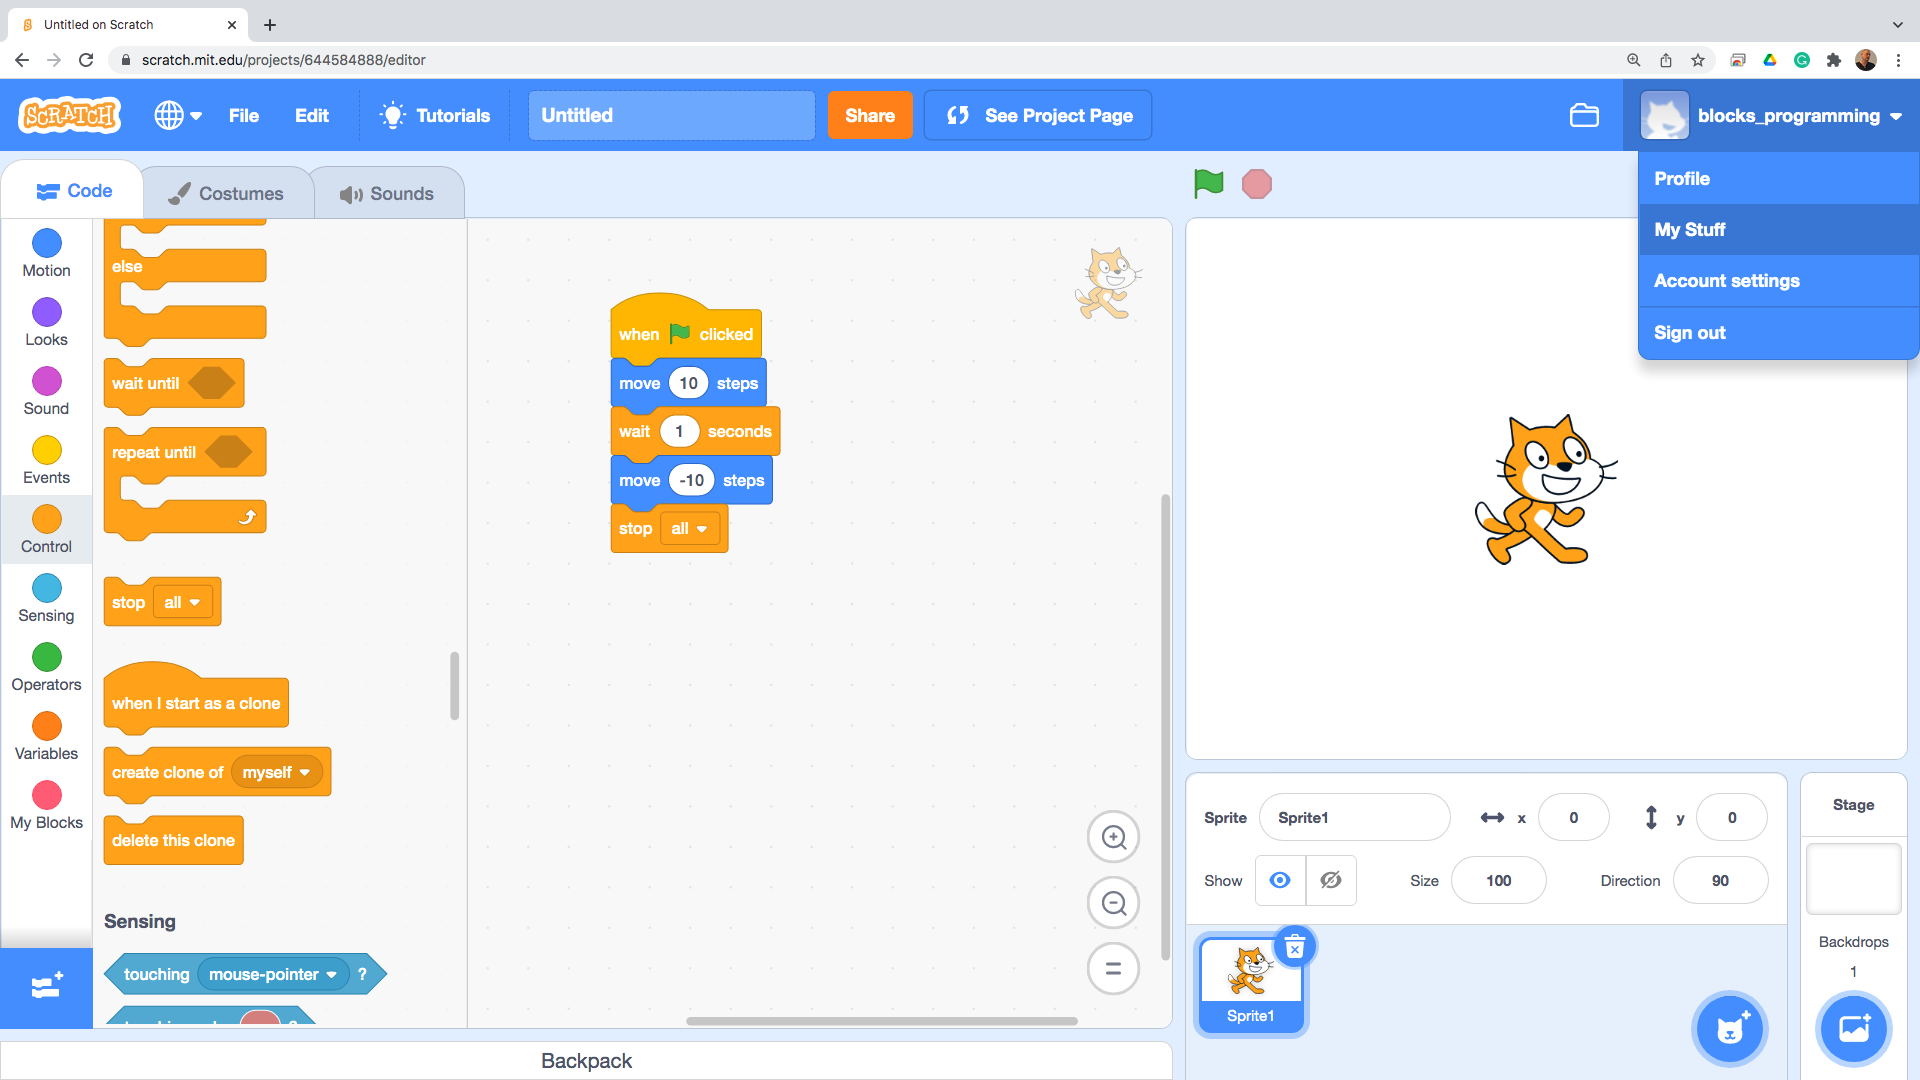
\includegraphics[width=1.0\linewidth,height=0.5\linewidth]{fig010019.png}
  \caption{Меню за организация на проектите}
\label{fig010019}
\end{figure}

Първоначално, всеки проект има служебно име (Фиг. \ref{fig010020}), което в последствие може да бъде променено. Едно от най-атрактивните предимства на програмната среда е, че проектите на потребителите могат да се споделят (Sharing) с много широка аудитория. Това позволява бърз трансфер на знания и умения, както и оценка за положения труд. 

\begin{figure}[H]
  \centering
  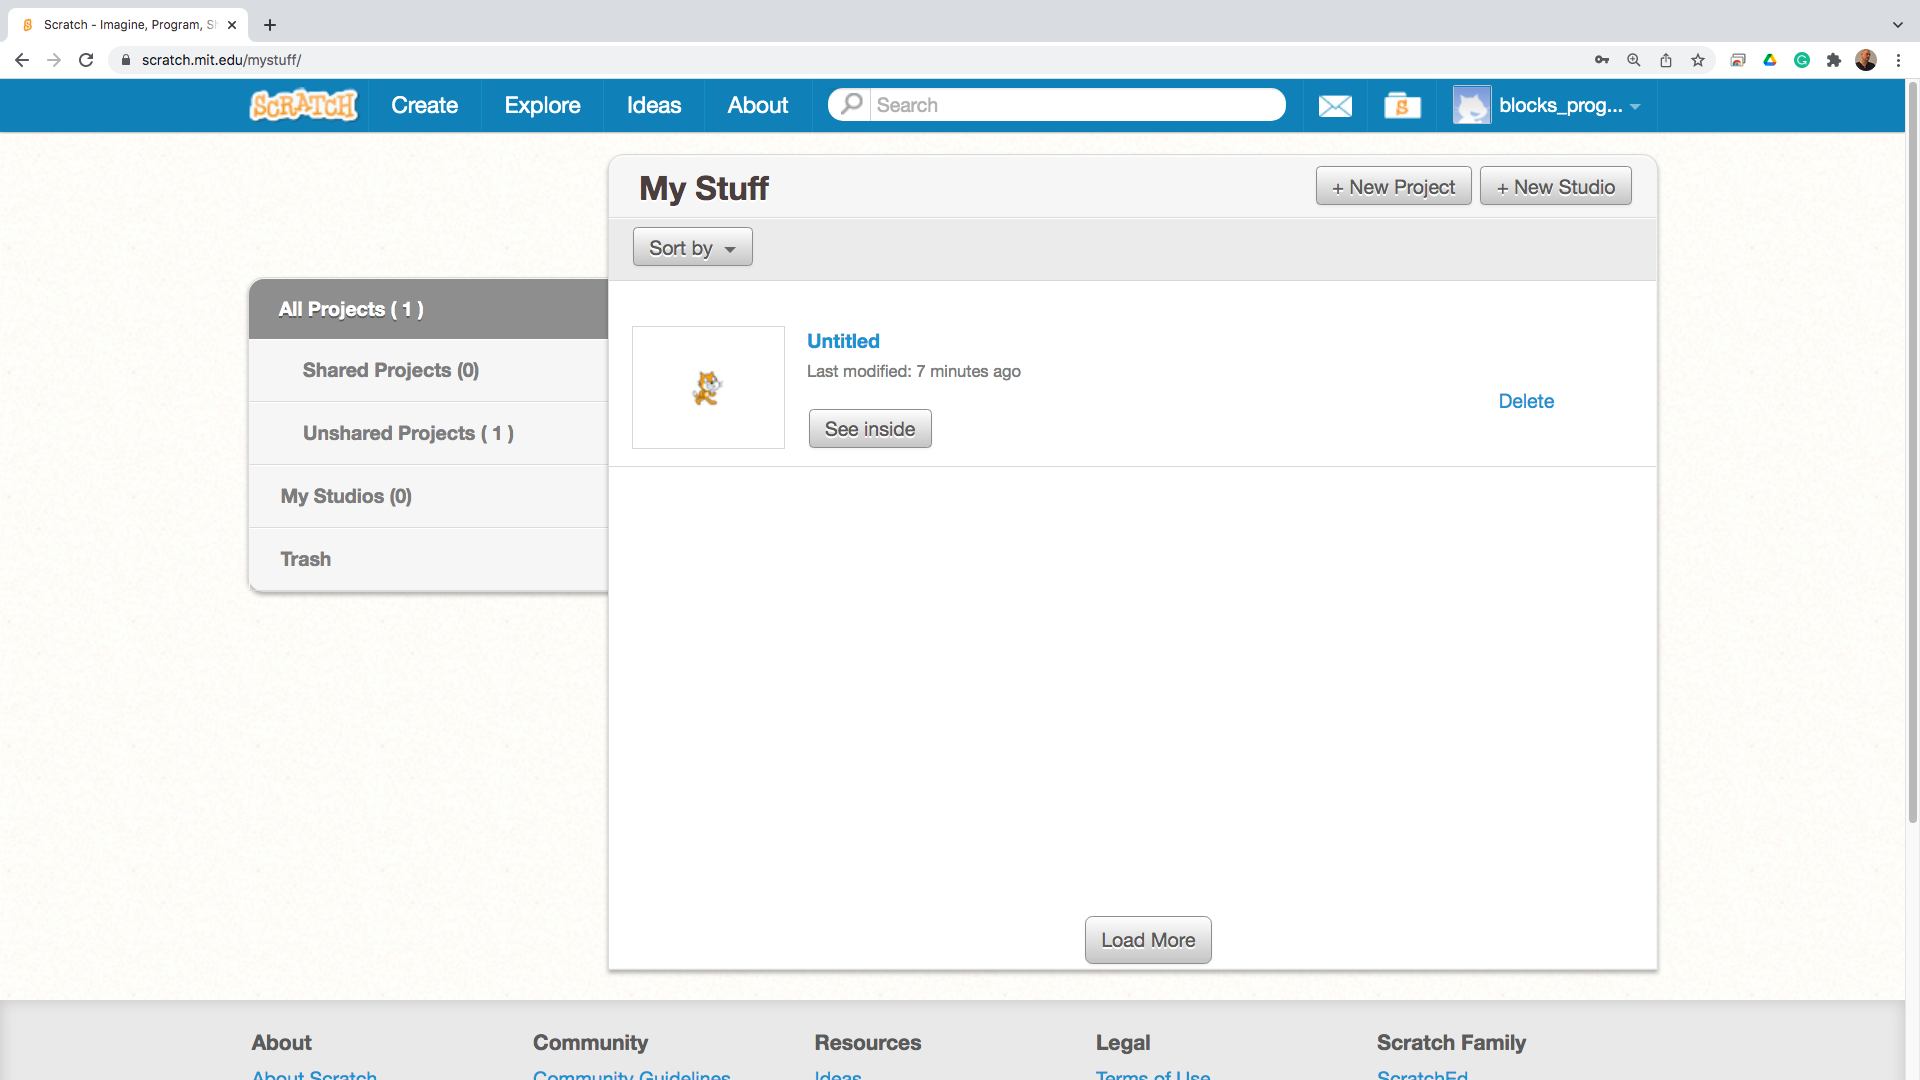
\includegraphics[width=1.0\linewidth,height=0.5\linewidth]{fig010020.png}
  \caption{Списък с проекти}
\label{fig010020}
\end{figure}

Най-голямото очарование блоковите езици получават от факта, че писането на инструкциите и формирането на цялостна програма прилича на подреждането на пъзел. Почти всички деца обичат да редят пазели. Харесват ярките цветове и красивите картини. Когато чарът на класическите пъзели се пренесе в една толкова атрактивна област, каквато е програмирането, резултатите могат да бъдат смайващи. 

\section{Първи стъпки в App Inventor}

Работата в средата на App Inventor започва със зареждане на главната уеб страница (Фиг. \ref{fig010021}), която се намира на адрес: \\ \href{https://appinventor.mit.edu/}{https://appinventor.mit.edu/}

\begin{figure}[H]
  \centering
  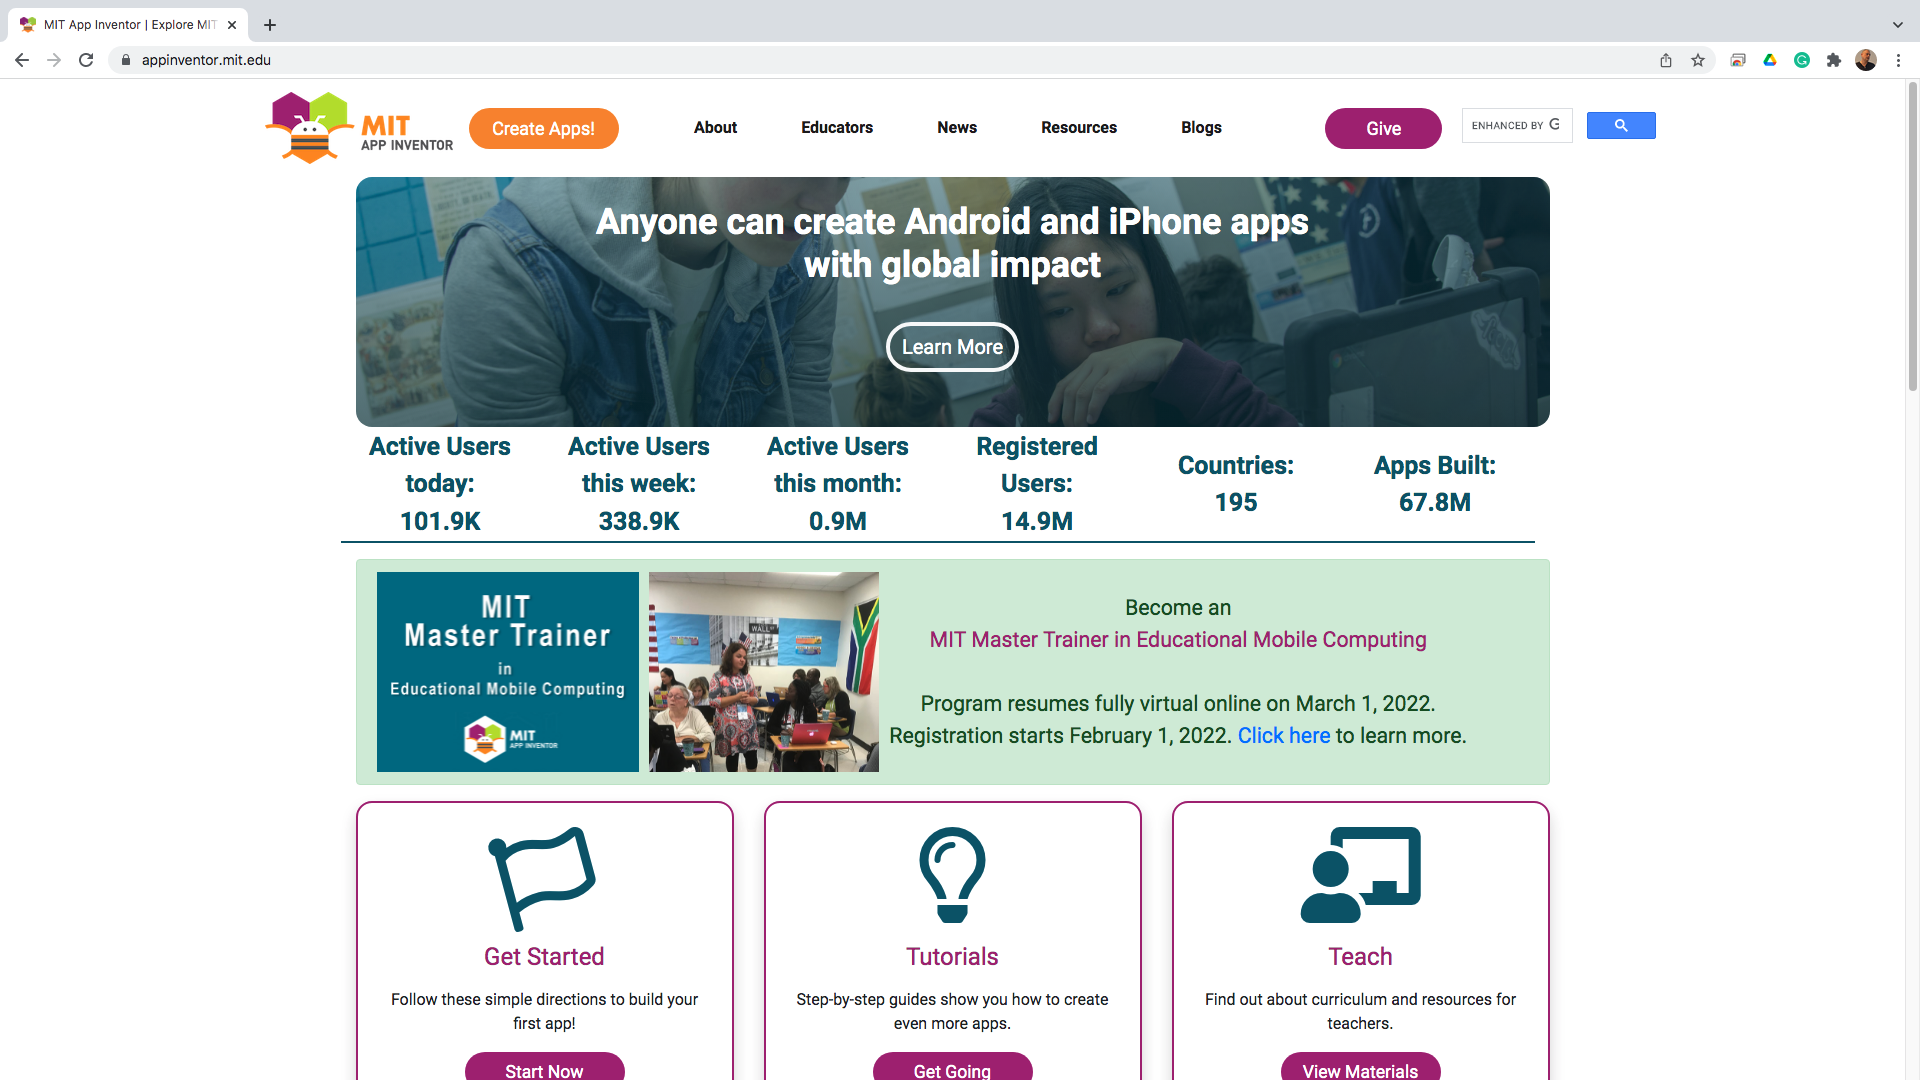
\includegraphics[width=1.0\linewidth,height=0.5\linewidth]{fig010021.png}
  \caption{Начална уеб страница на App Inventor}
\label{fig010021}
\end{figure}

Въпреки че App Inventor също е продукт на Масачузетския технологичен институт в някои аспекти работата с него се различава от начина по който се работи в Scratch. App Inventor също се предлага под формата на облачна услуга в която е необходима регистрация. За разлика от  Scratch, в App Inventor може да се пропусне създаването на потребителски профил, а влизането в системата да се осъществи, чрез класическа регистрация в услугата GMail. Този процес започва след избирането на оранжевия бутон „Create Apps!“ (Фиг. \ref{fig010022}).

\begin{figure}[H]
  \centering
  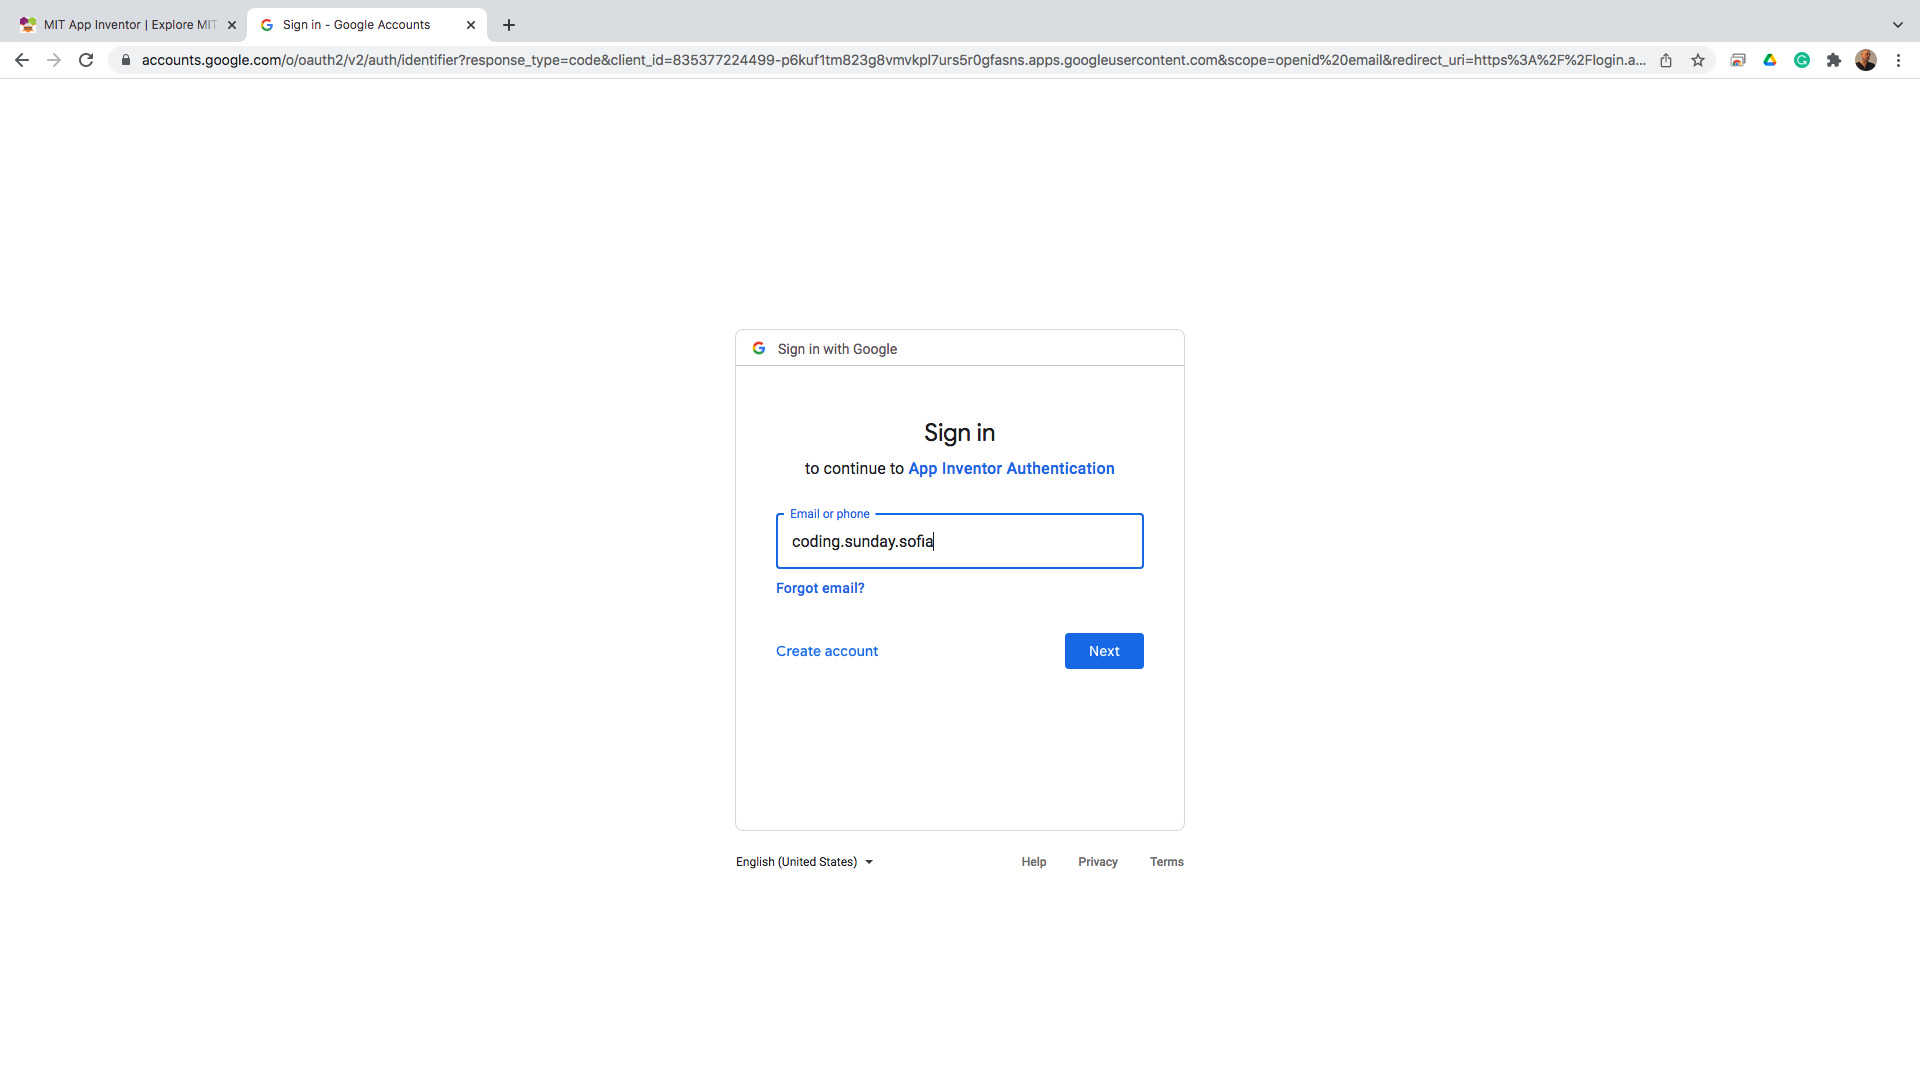
\includegraphics[width=1.0\linewidth,height=0.5\linewidth]{fig010022.png}
  \caption{Избор на GMail потребител за включване в системата}
\label{fig010022}
\end{figure}

След избора на потребител, с който да се работи в средата на App Inventor е нужно този потребител да се автентифицира, чрез въвеждане на парола (Фиг. \ref{fig010023}).

\begin{figure}[H]
  \centering
  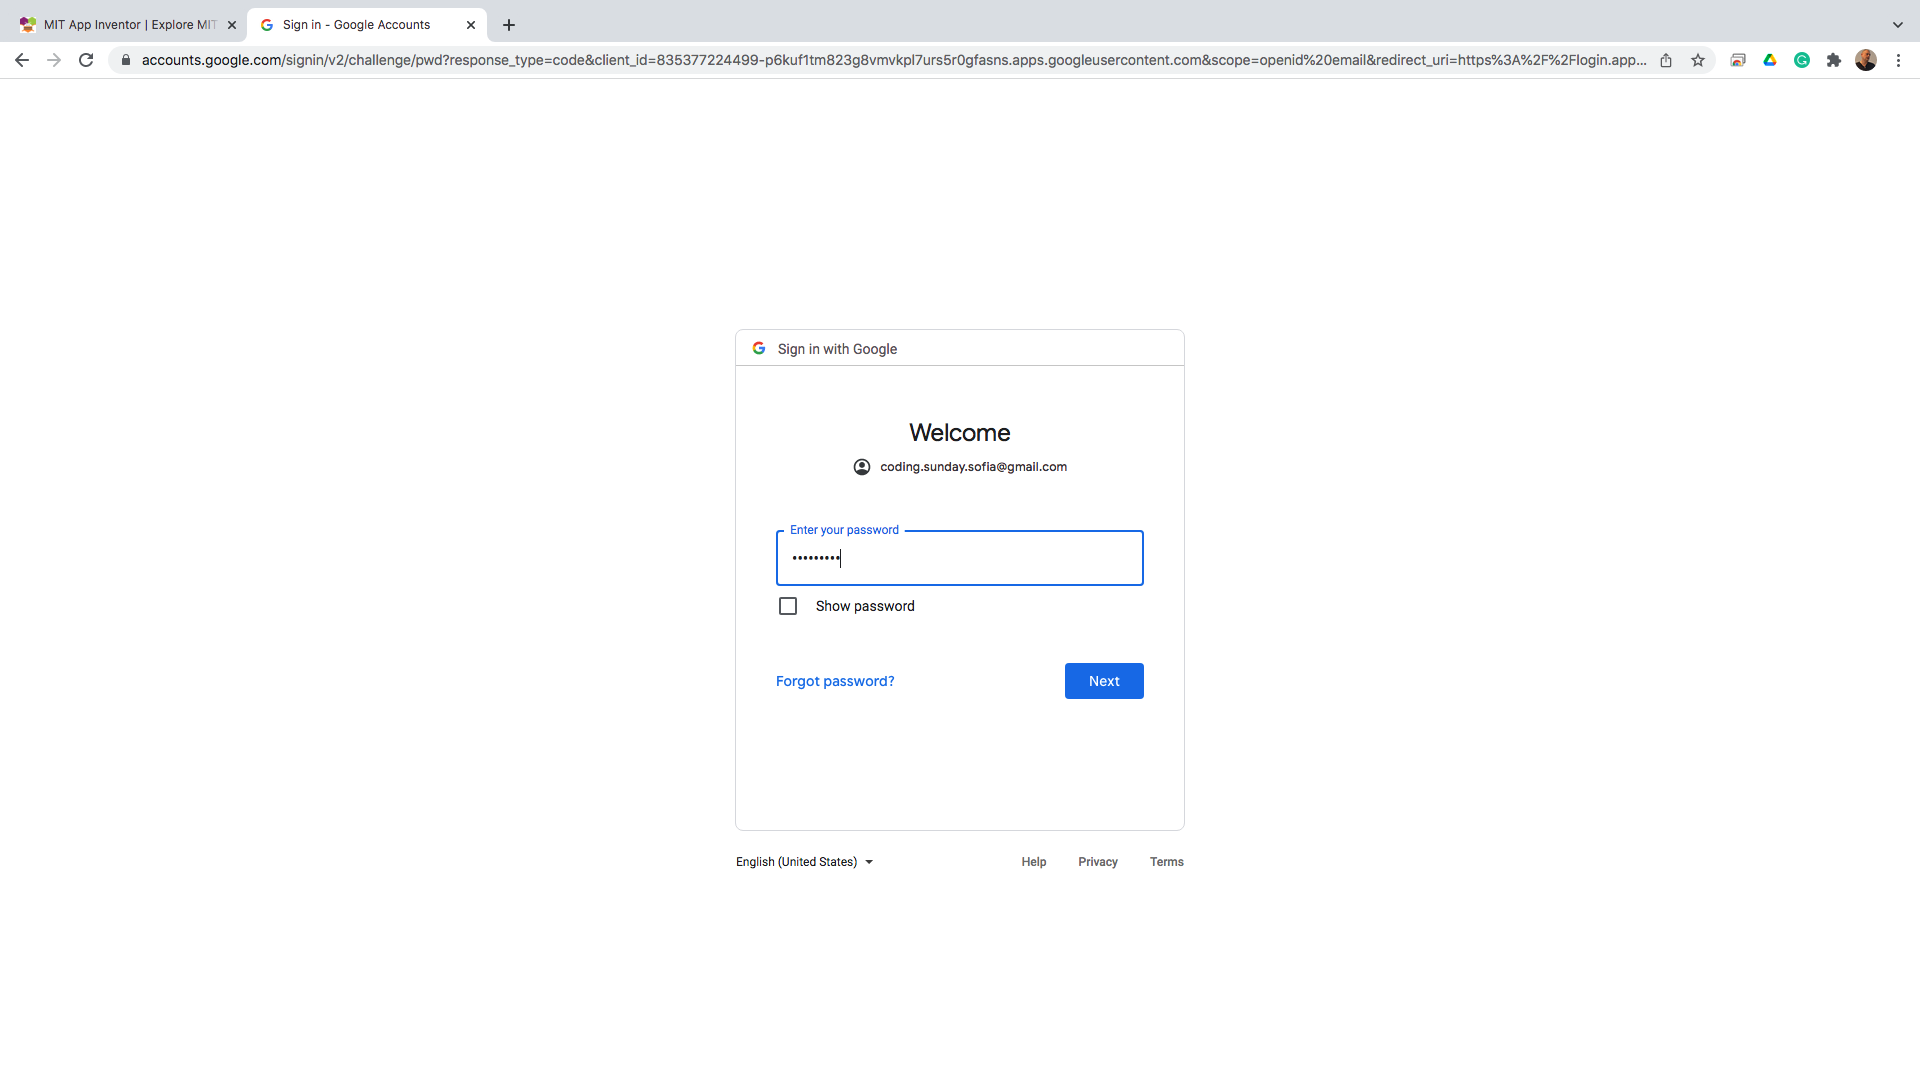
\includegraphics[width=1.0\linewidth,height=0.5\linewidth]{fig010023.png}
  \caption{Автентификация на потребителя}
\label{fig010023}
\end{figure}

За да бъде позволена работа в програмната среда на App Inventor се изисква съгласие от потребителя с общите условия на платформата (Фиг. \ref{fig010024}).

\begin{figure}[H]
  \centering
  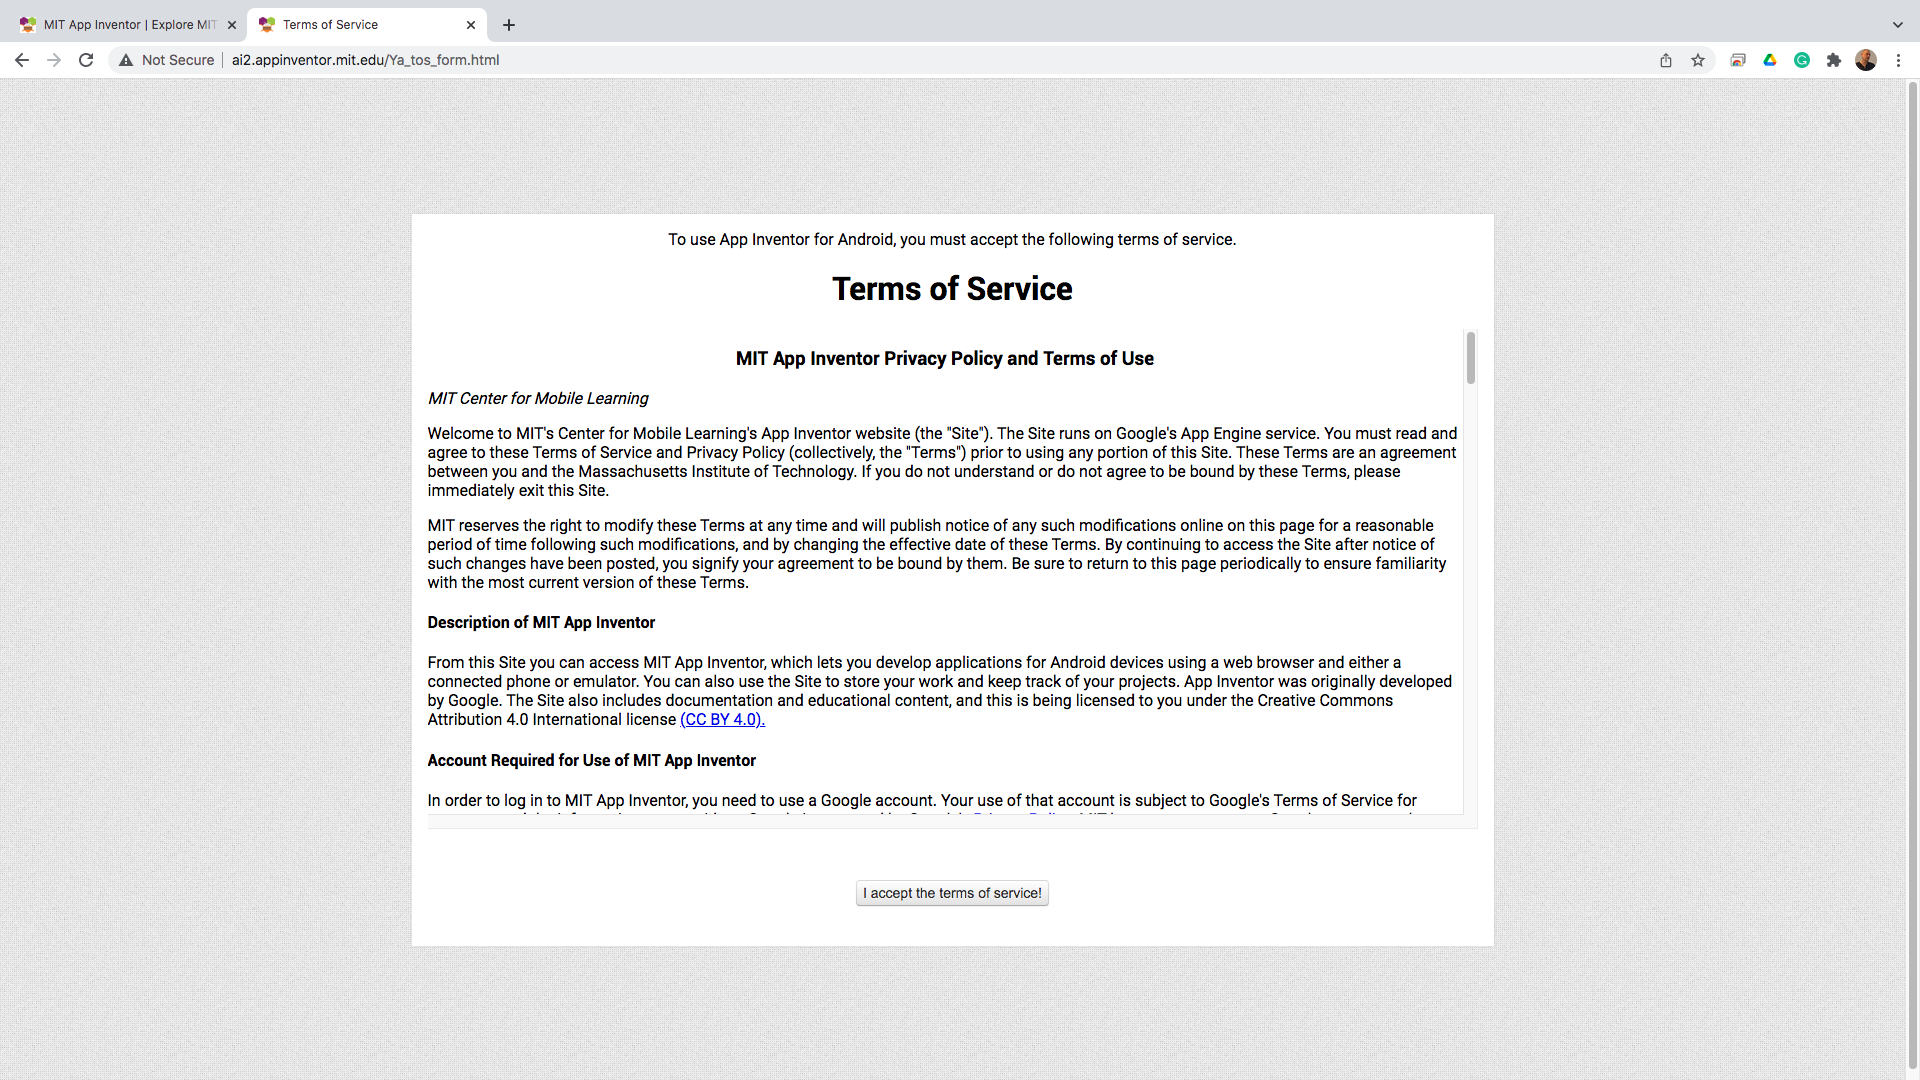
\includegraphics[width=1.0\linewidth,height=0.5\linewidth]{fig010024.png}
  \caption{Общи условия за ползване на програмната среда}
\label{fig010024}
\end{figure}

Процесът по вход в програмната среда завършва с поздравителна уеб страница (Фиг. \ref{fig010025}). На тази страница е представена по-подробна информация за програмната среда, видът на стартираната инстанция и версия. 

\begin{figure}[H]
  \centering
  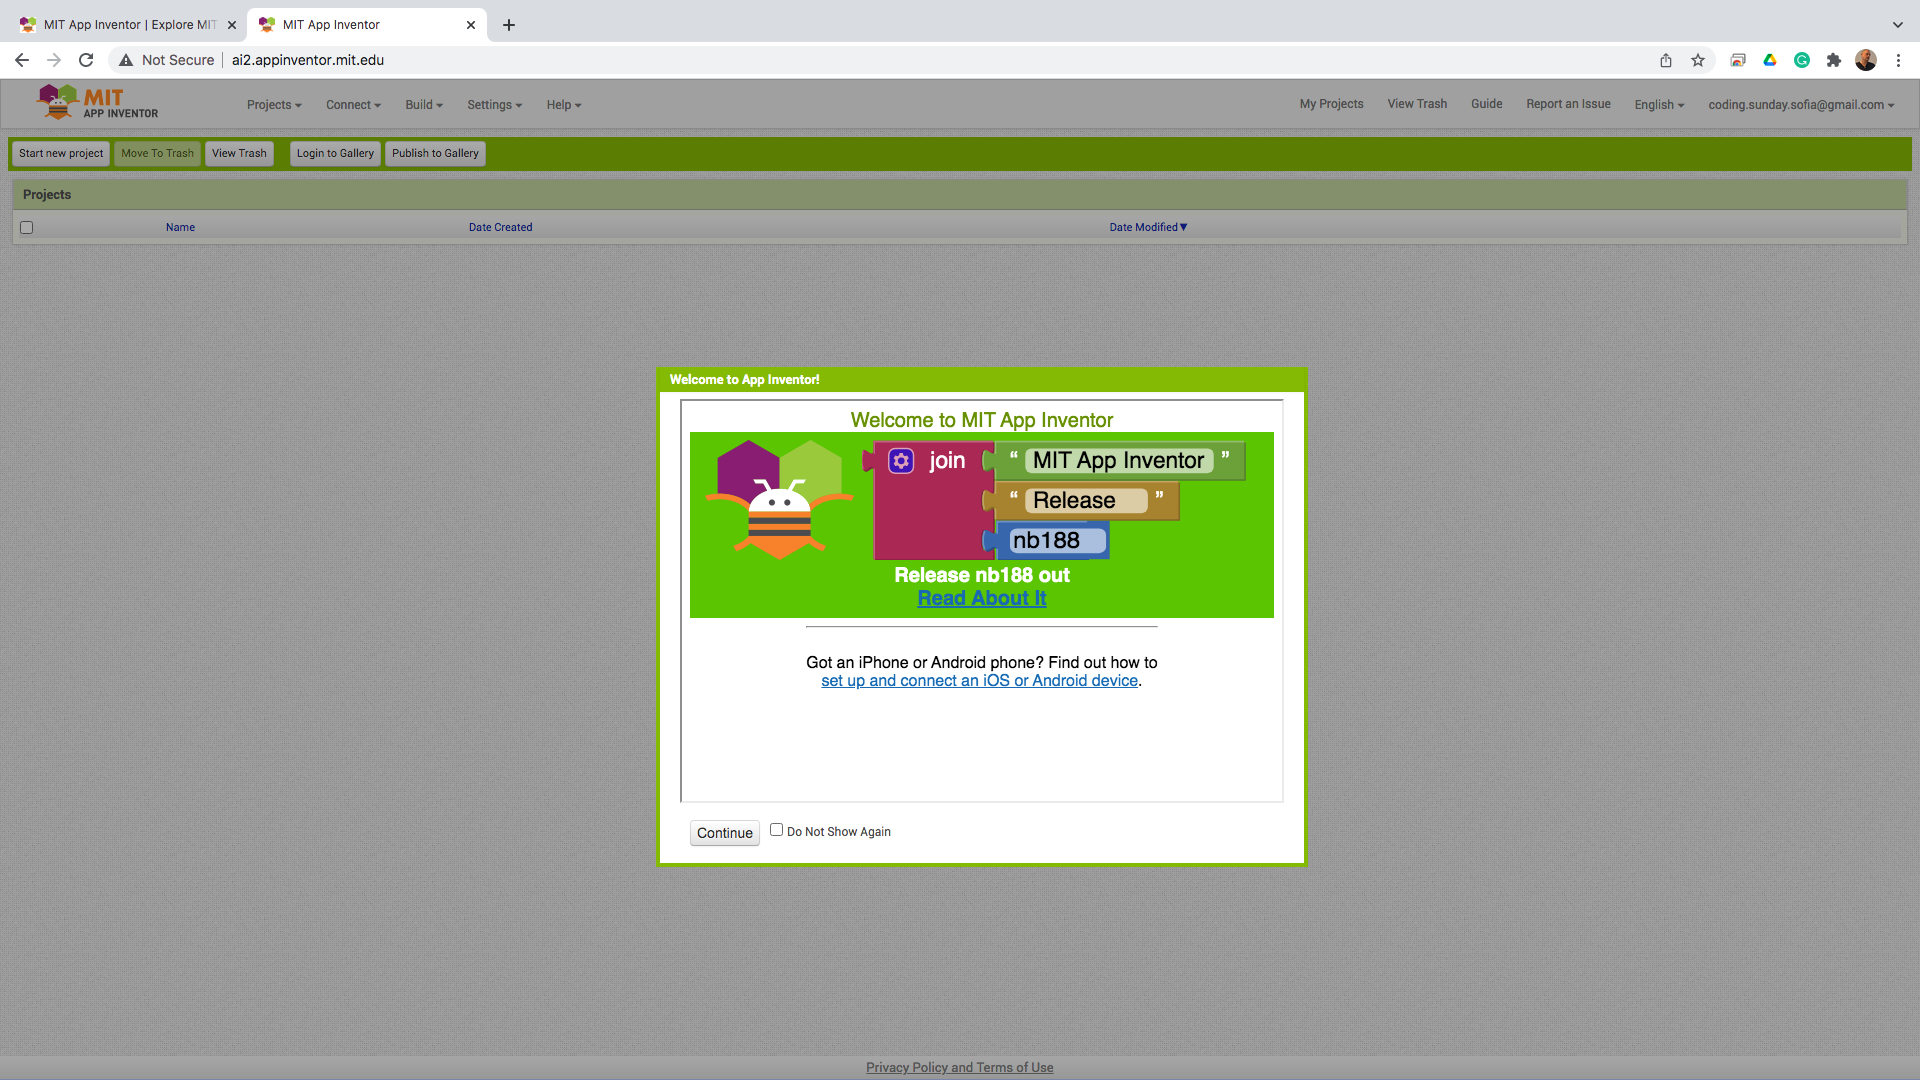
\includegraphics[width=1.0\linewidth,height=0.5\linewidth]{fig010025.png}
  \caption{Поздравителна страница}
\label{fig010025}
\end{figure}

Първата възможност, която се предлага на потребителя е да избере от възможности за разглеждане на няколко учебни проекта, служещи за първоначално въвеждане в начина за работа с програмната среда (Фиг. \ref{fig010026}).

\begin{figure}[H]
  \centering
  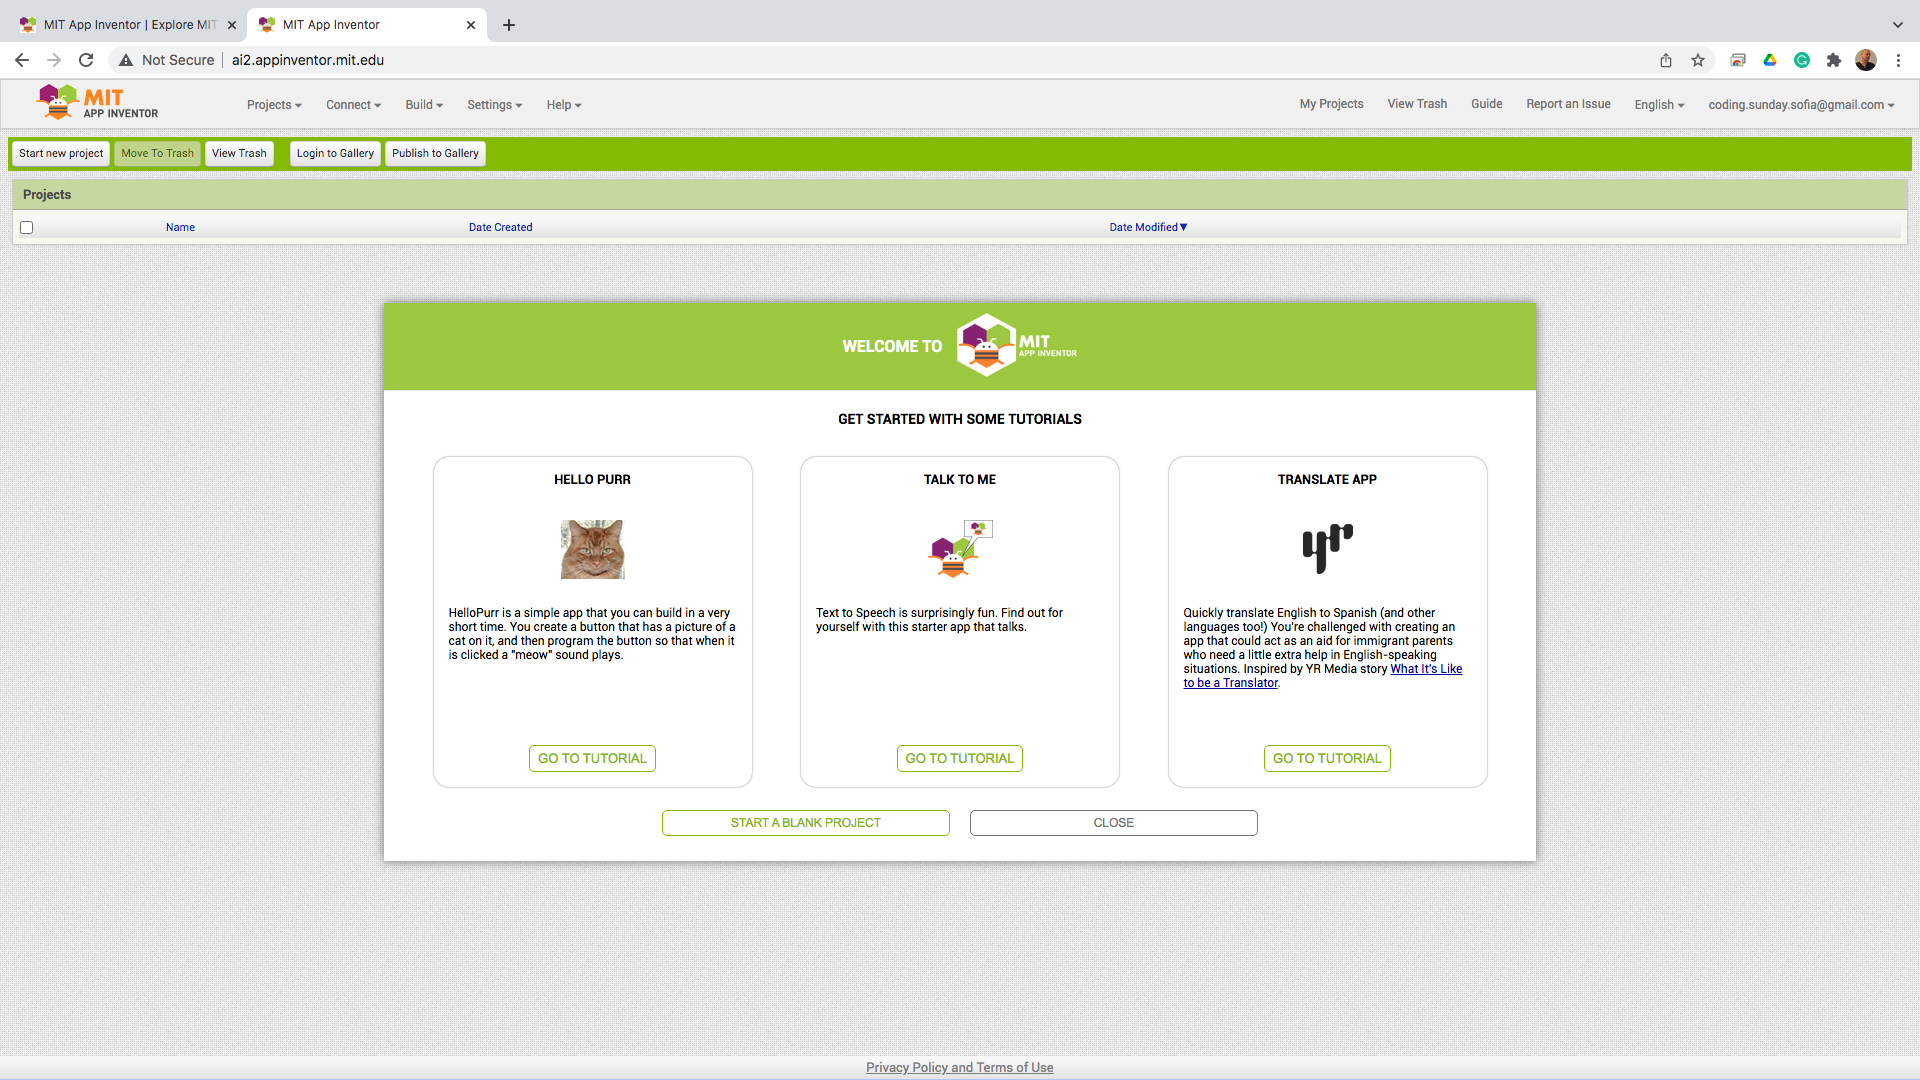
\includegraphics[width=1.0\linewidth,height=0.5\linewidth]{fig010026.png}
  \caption{Възможност за избор на учебни проекти}
\label{fig010026}
\end{figure}

Ако не бъде избран учебен проект или опцията за създаване на празен проект, системата насочва потребителя към страницата със списък от собствени проекти (Фиг. \ref{fig010027}).

\begin{figure}[H]
  \centering
  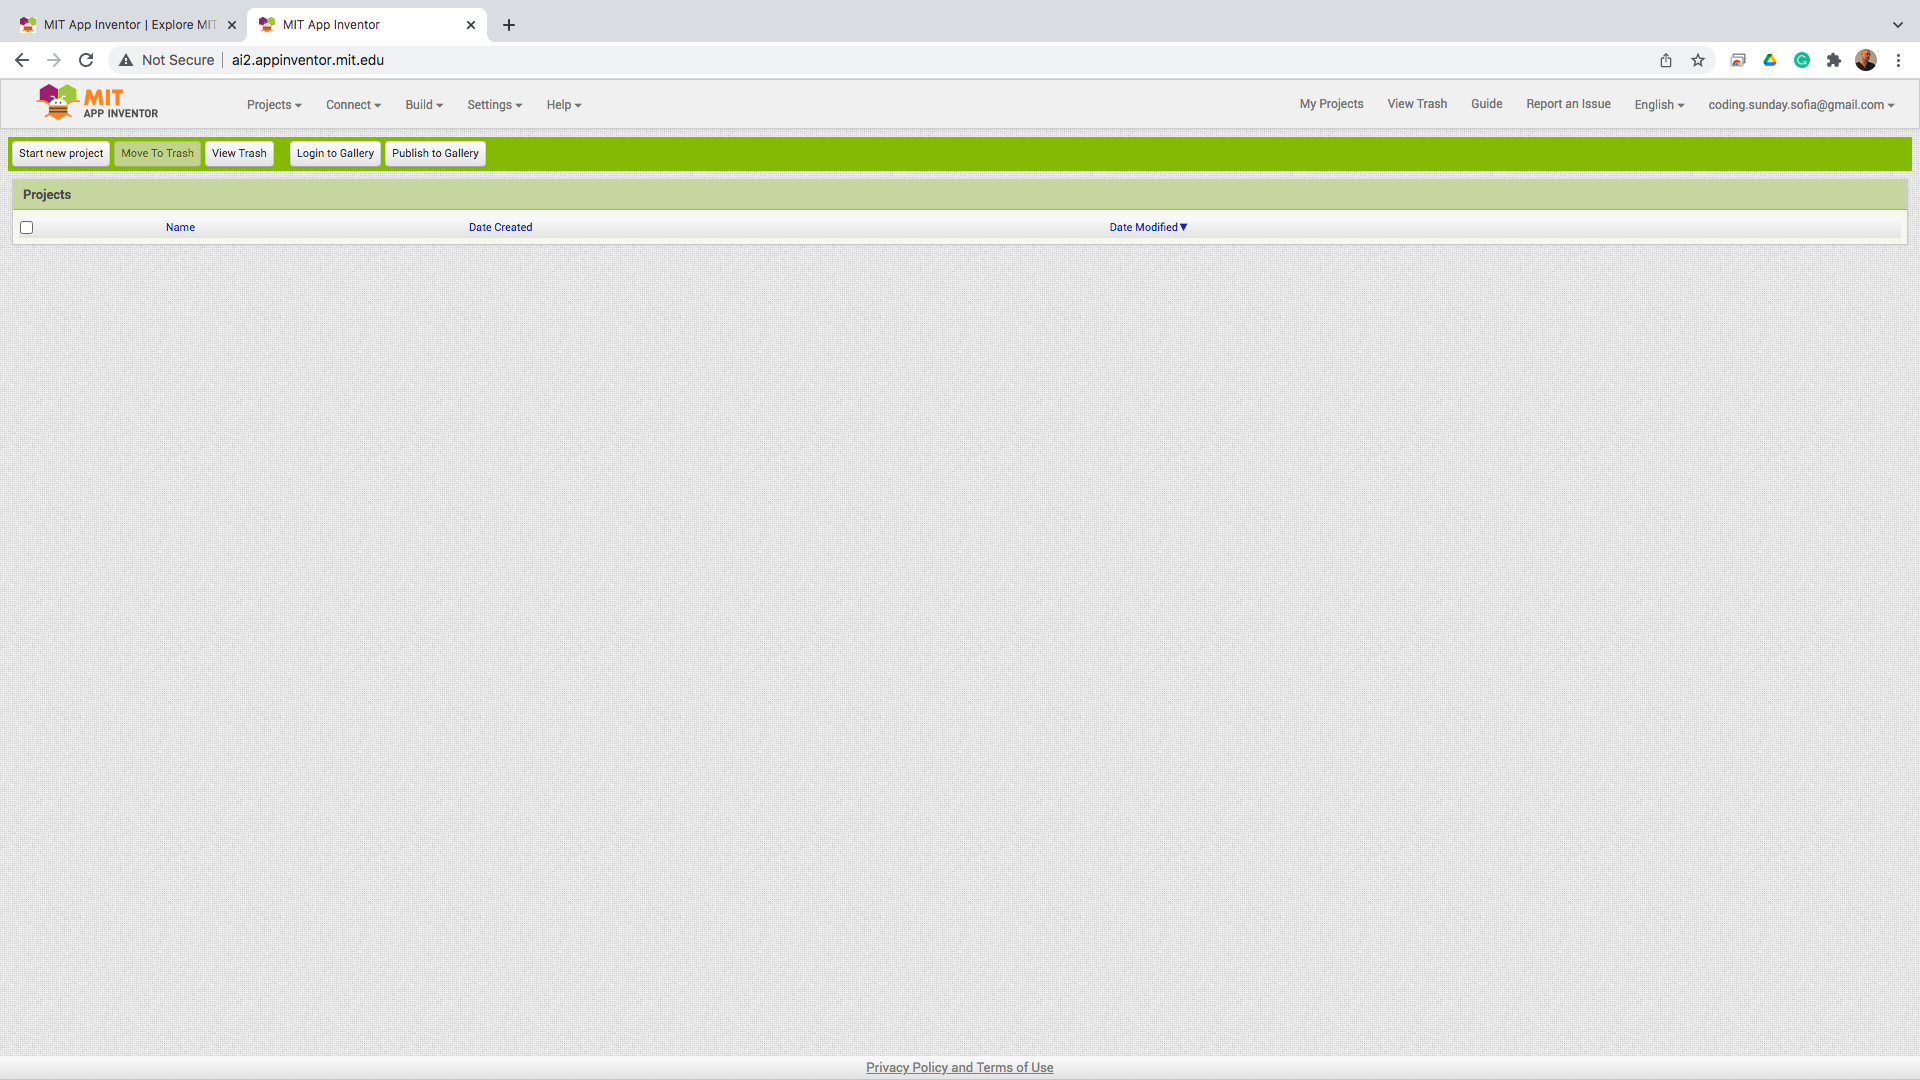
\includegraphics[width=1.0\linewidth,height=0.5\linewidth]{fig010027.png}
  \caption{Страница със списък от собствени проекти}
\label{fig010027}
\end{figure}

Започването на нов проект се случва от бутон, горе в ляво, на основният работен екран (Фиг. \ref{fig010028}).

\begin{figure}[H]
  \centering
  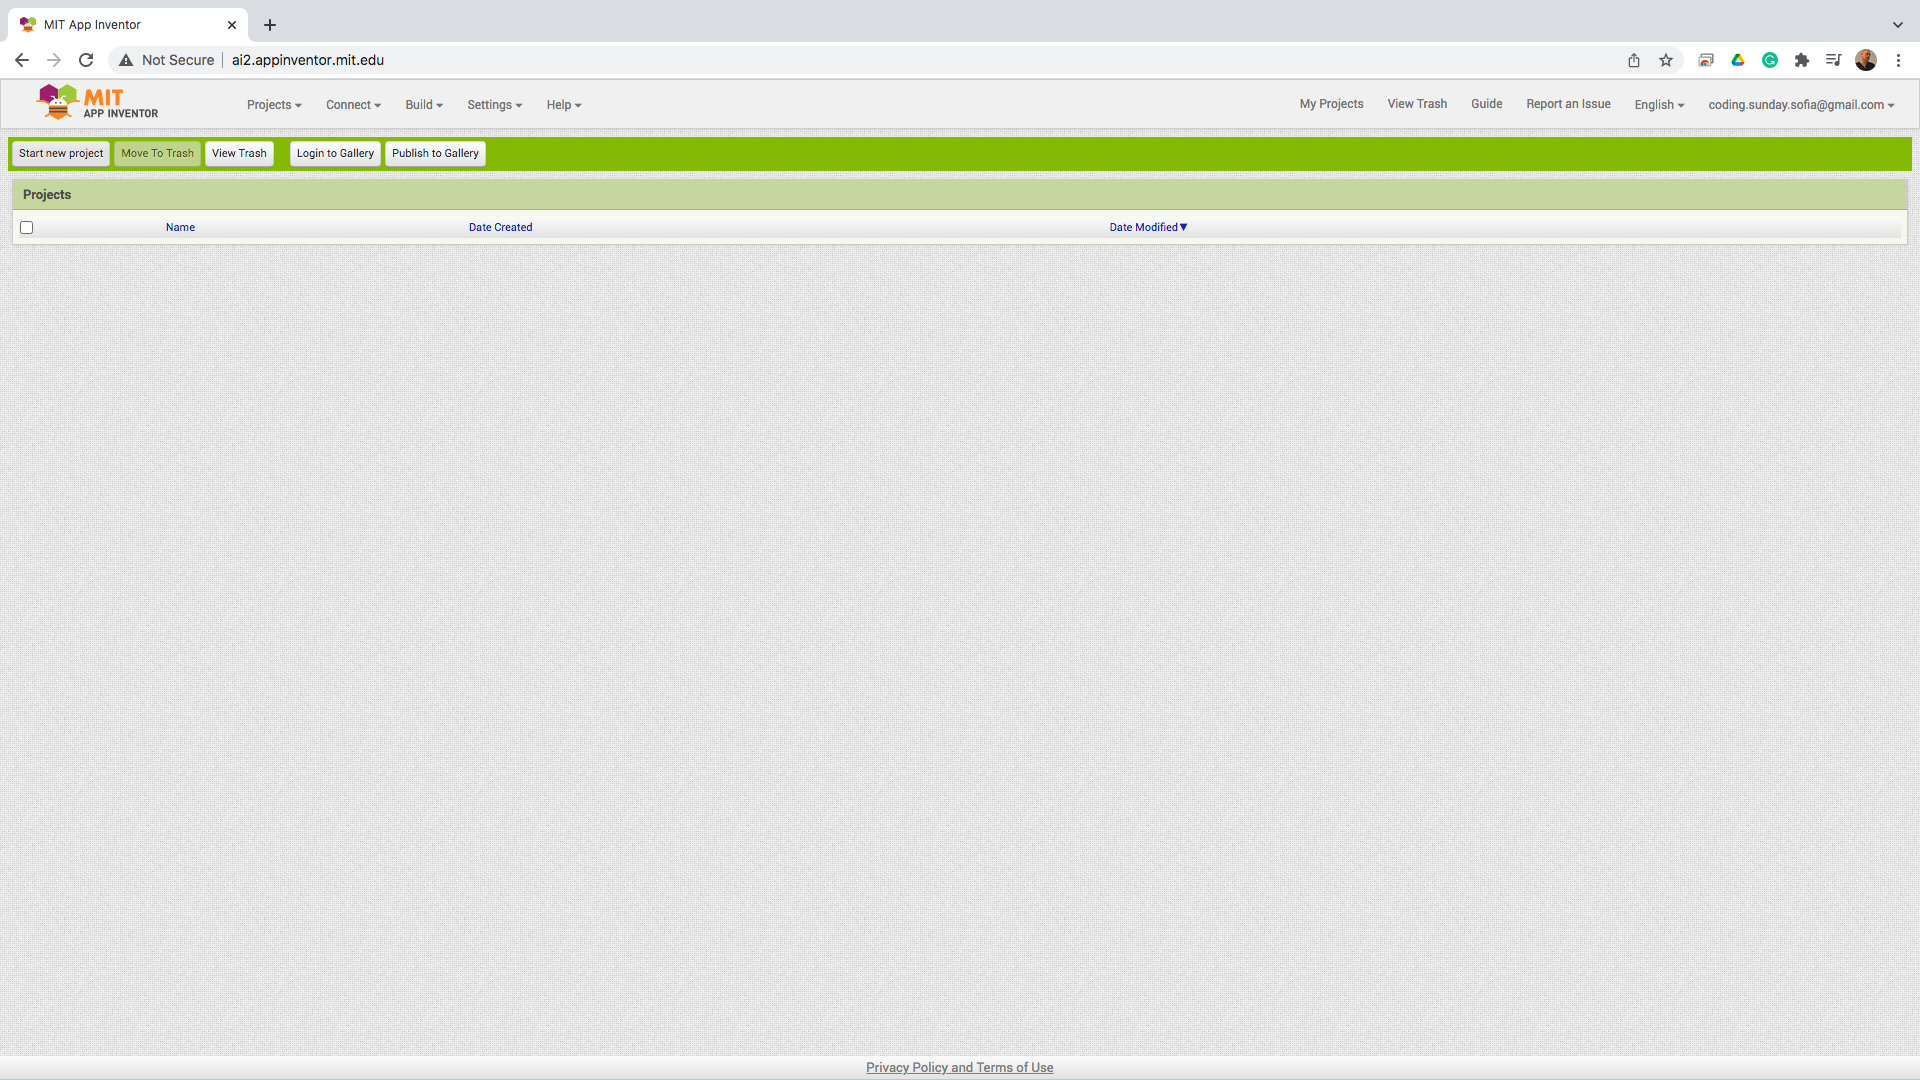
\includegraphics[width=1.0\linewidth,height=0.5\linewidth]{fig010028.png}
  \caption{Бутон за стартиране на нов проект}
\label{fig010028}
\end{figure}

Програмната среда на App Inventor организира работата върху програмен код под формата на проекти. Всеки проект трябва да има подходящо название, което се задава още при създаването на проекта (Фиг. \ref{fig010029}).

\begin{figure}[H]
  \centering
  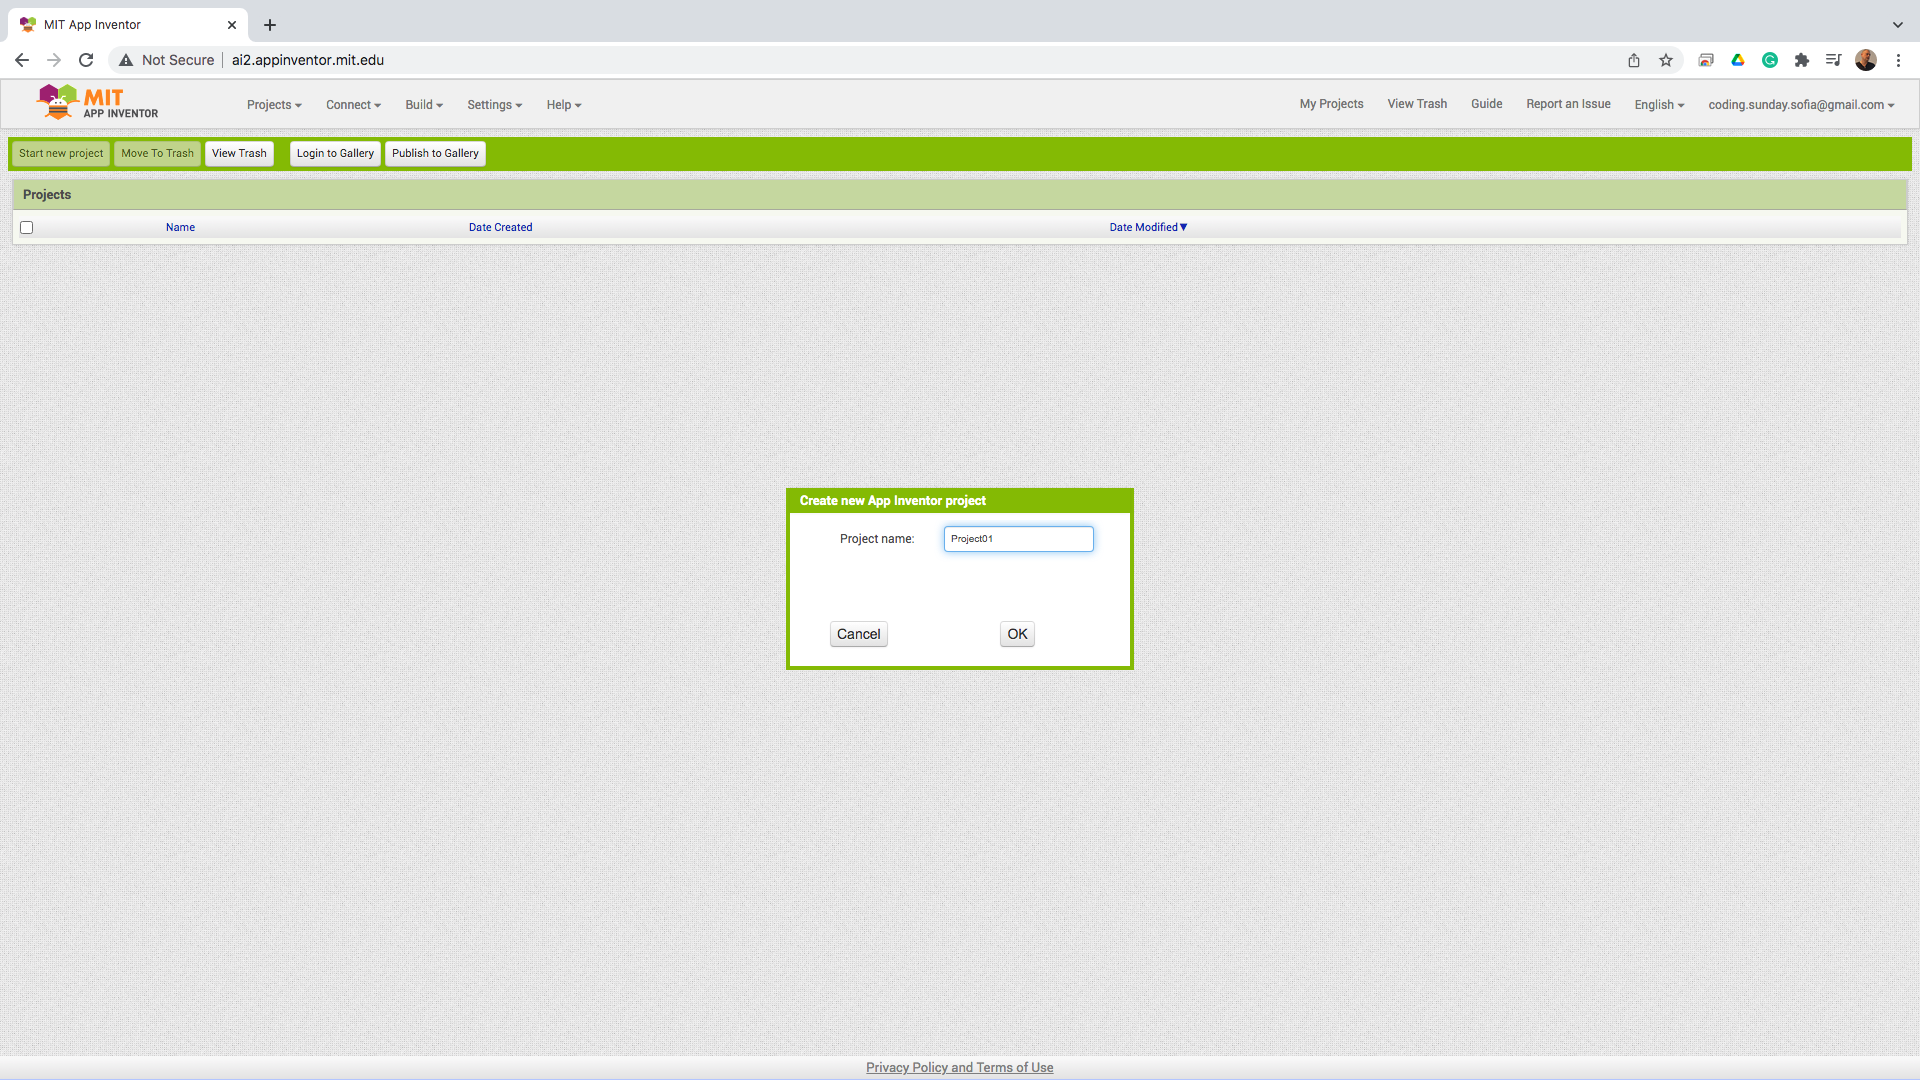
\includegraphics[width=1.0\linewidth,height=0.5\linewidth]{fig010029.png}
  \caption{Название на проекта}
\label{fig010029}
\end{figure}

След избора на название, програмната среда визуализира първият работен екран, даващ възможност за проектиране на визуалния потребителски интерфейс (Фиг. \ref{fig010030}). Проектирането на визуалния потребителски интерфейс се случва, чрез придърпване на различните визуални контроли в основната работна площ. 

\begin{figure}[H]
  \centering
  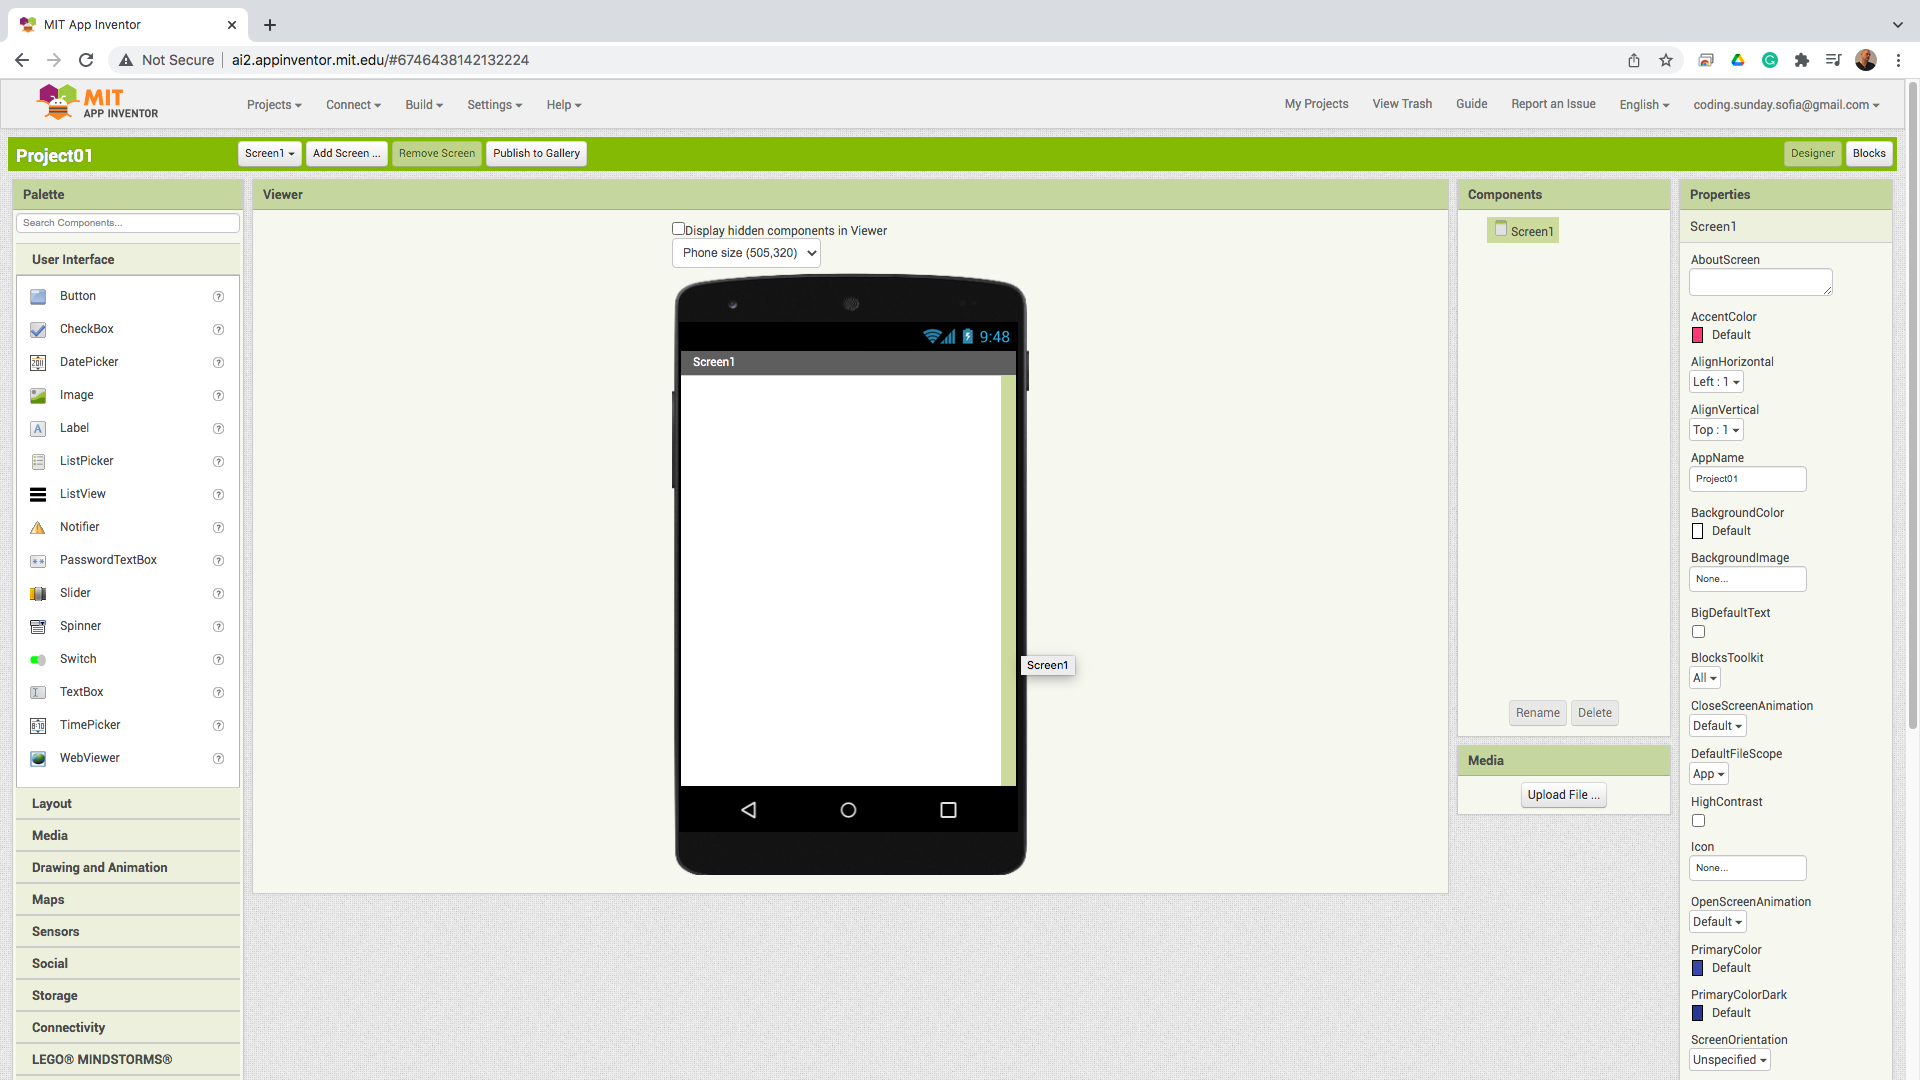
\includegraphics[width=1.0\linewidth,height=0.5\linewidth]{fig010030.png}
  \caption{Проектантски изглед на развойната среда}
\label{fig010030}
\end{figure}

Един от най-базовите визуални контроли е бутонът. Представлява обособена зона във визуалното поле, която има текстово надписване или икона за визуално представяне на действието, извършвано след натискането на бутона. За демонстрирането на процеса по работа със съставения програмен код се използва един бутон (Фиг. \ref{fig010031}).

\begin{figure}[H]
  \centering
  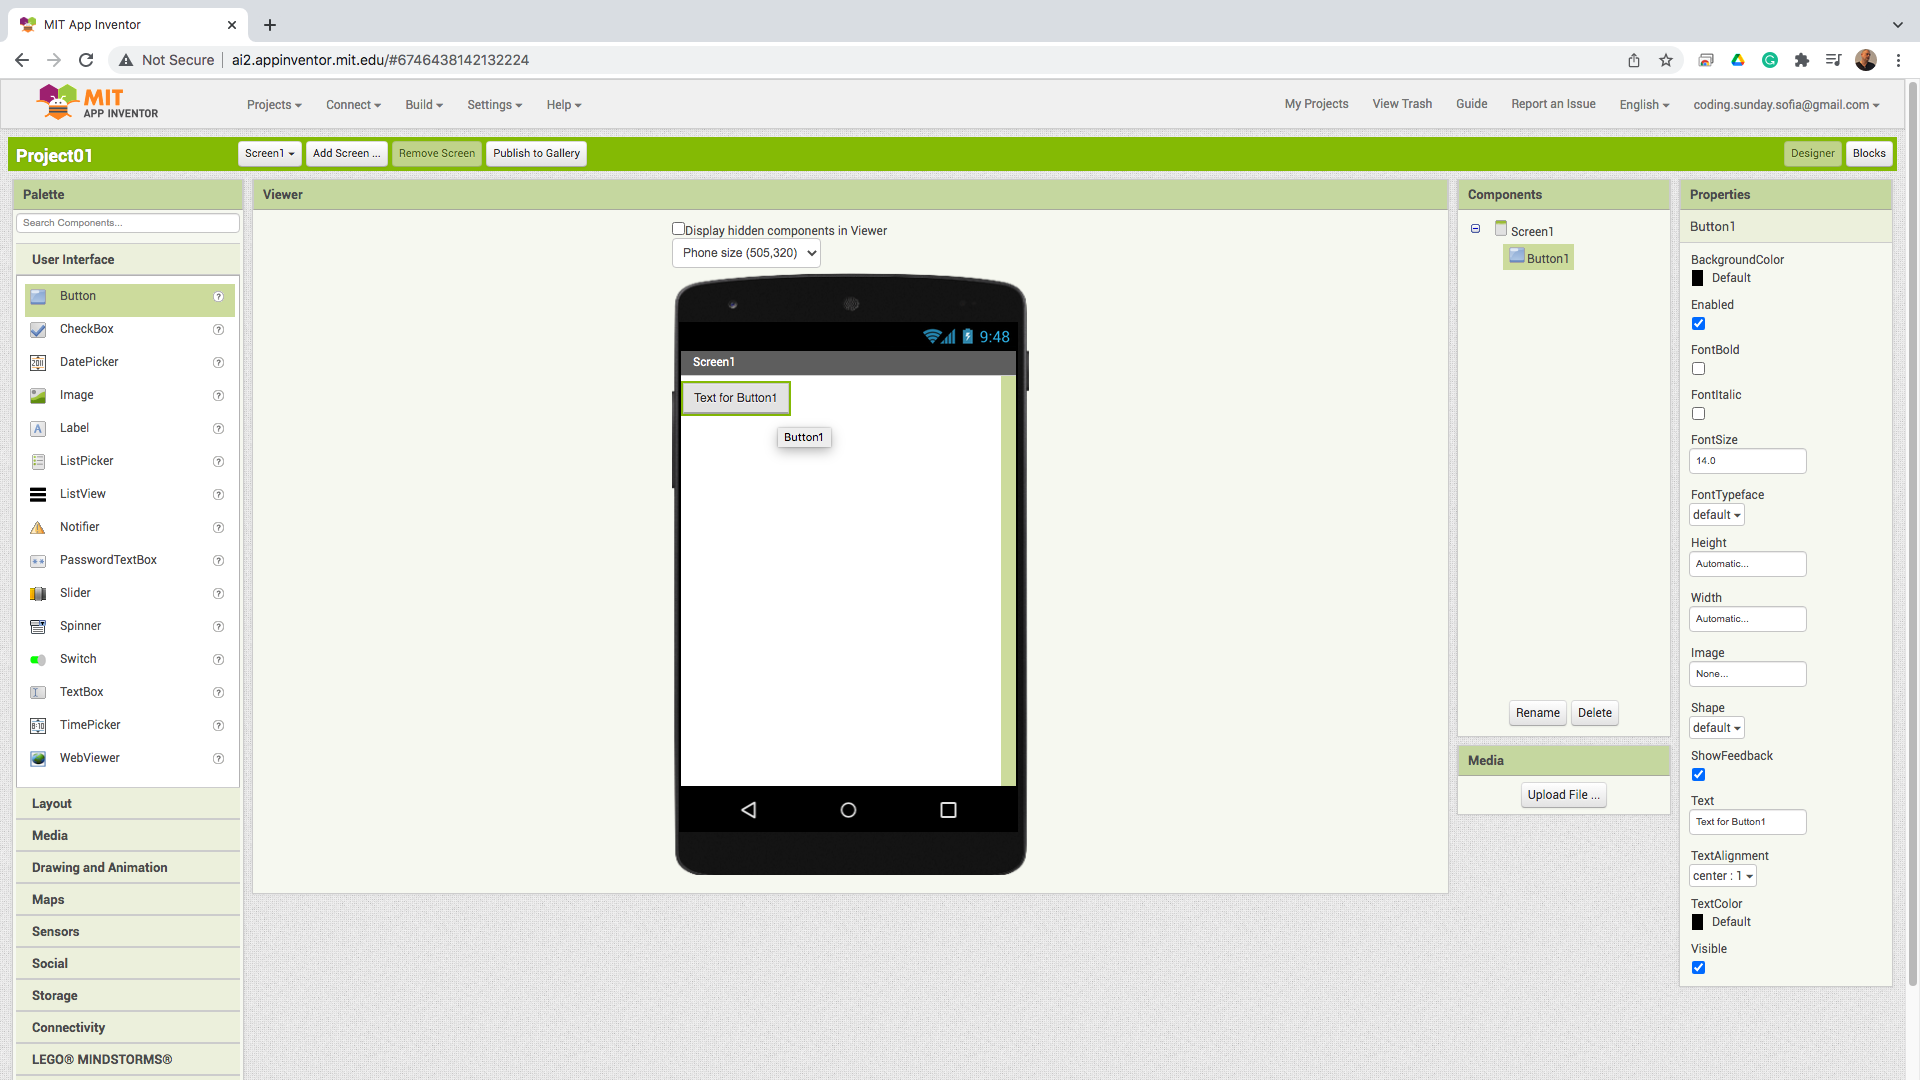
\includegraphics[width=1.0\linewidth,height=0.5\linewidth]{fig010031.png}
  \caption{Поставяне на бутон}
\label{fig010031}
\end{figure}

От съществено значение е за хората използващи софтуерното приложение, бутоните да имат максимално експресивни названия. В случая, целта е бутонът да бъде натиснат и от това да последва конкретно действие. Поради тази причина, названието на бутона е само „Push“ (Фиг. \ref{fig010031}).

\begin{figure}[H]
  \centering
  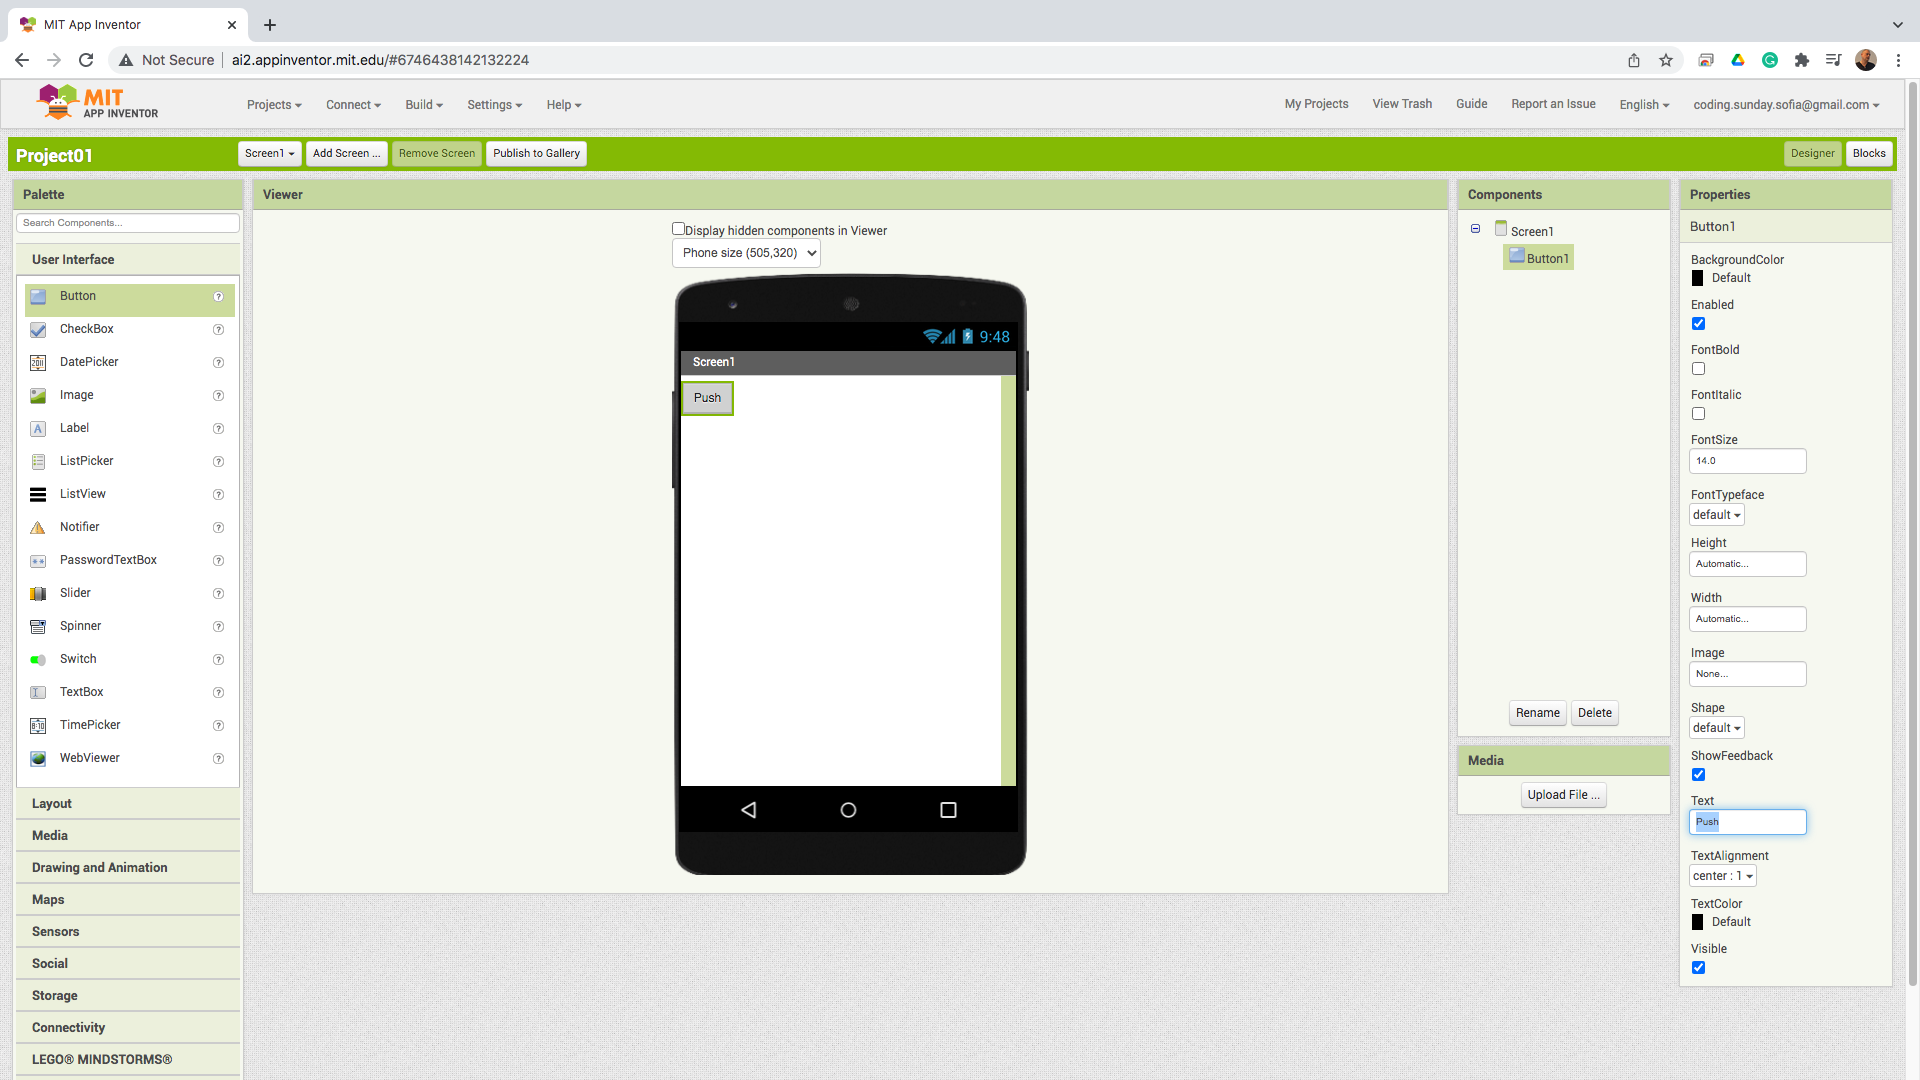
\includegraphics[width=1.0\linewidth,height=0.5\linewidth]{fig010032.png}
  \caption{Избор на текст върху бутона}
\label{fig010032}
\end{figure}

За разлика от програмната среда Scratch, при App Inventor програмните инструкции се подрежат под формата на пъзел в отделен работен екран (Фиг. \ref{fig010033}). 

\begin{figure}[H]
  \centering
  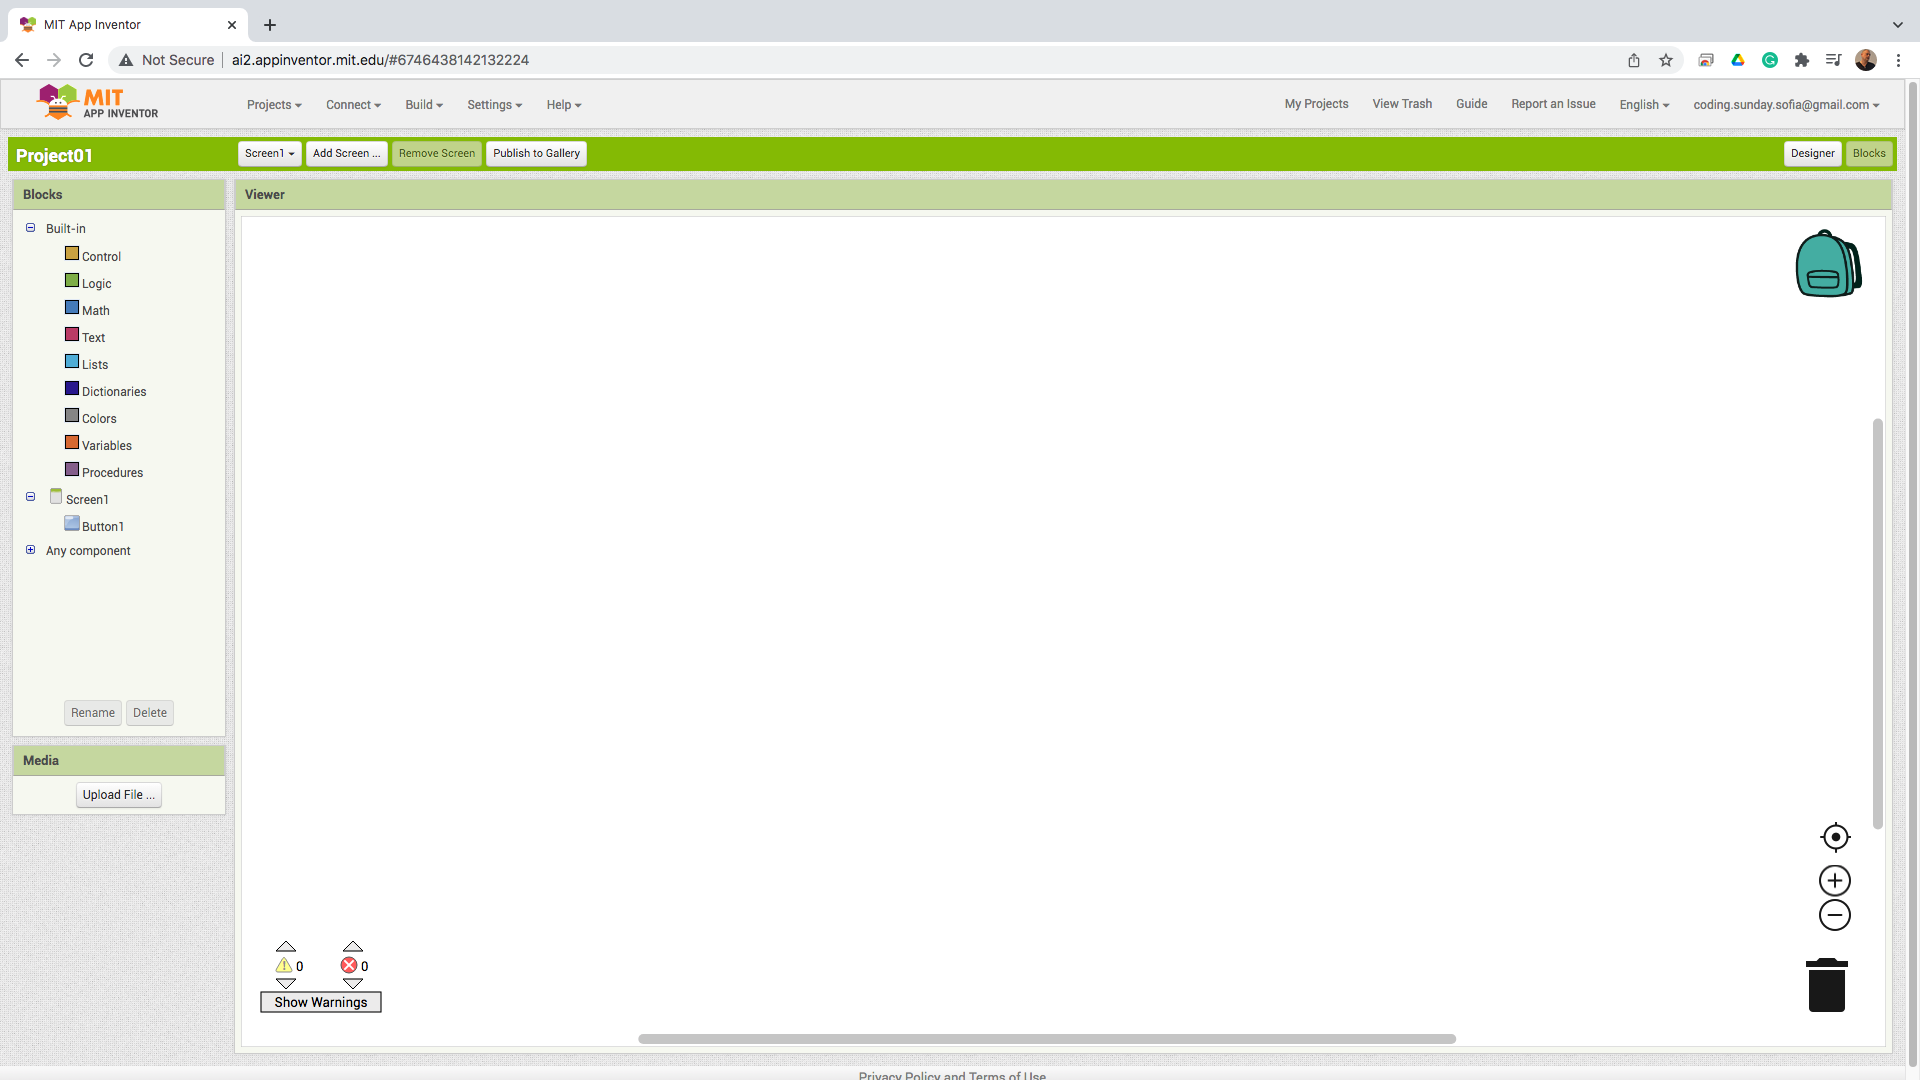
\includegraphics[width=1.0\linewidth,height=0.5\linewidth]{fig010033.png}
  \caption{Програмен изглед на развойната среда}
\label{fig010033}
\end{figure}

Тъй като графичният потребителски интерфейс до момента се състои само от единствен компонент (бутон), то някакви инструкции могат да се изпълнят единствено с този визуален компонент. За разлика от Scratch, където програмата има начална стартова точка и финална крайна точка, при App Inventor програмните инструкции се подреждат на принципа на възникващите събития. Когато програмата започне да работи, тя визуализира графичния потребителски интерфейс и очаква от ползващия устройството да извърши някакво действие (Фиг. \ref{fig010034}). 

\begin{figure}[H]
  \centering
  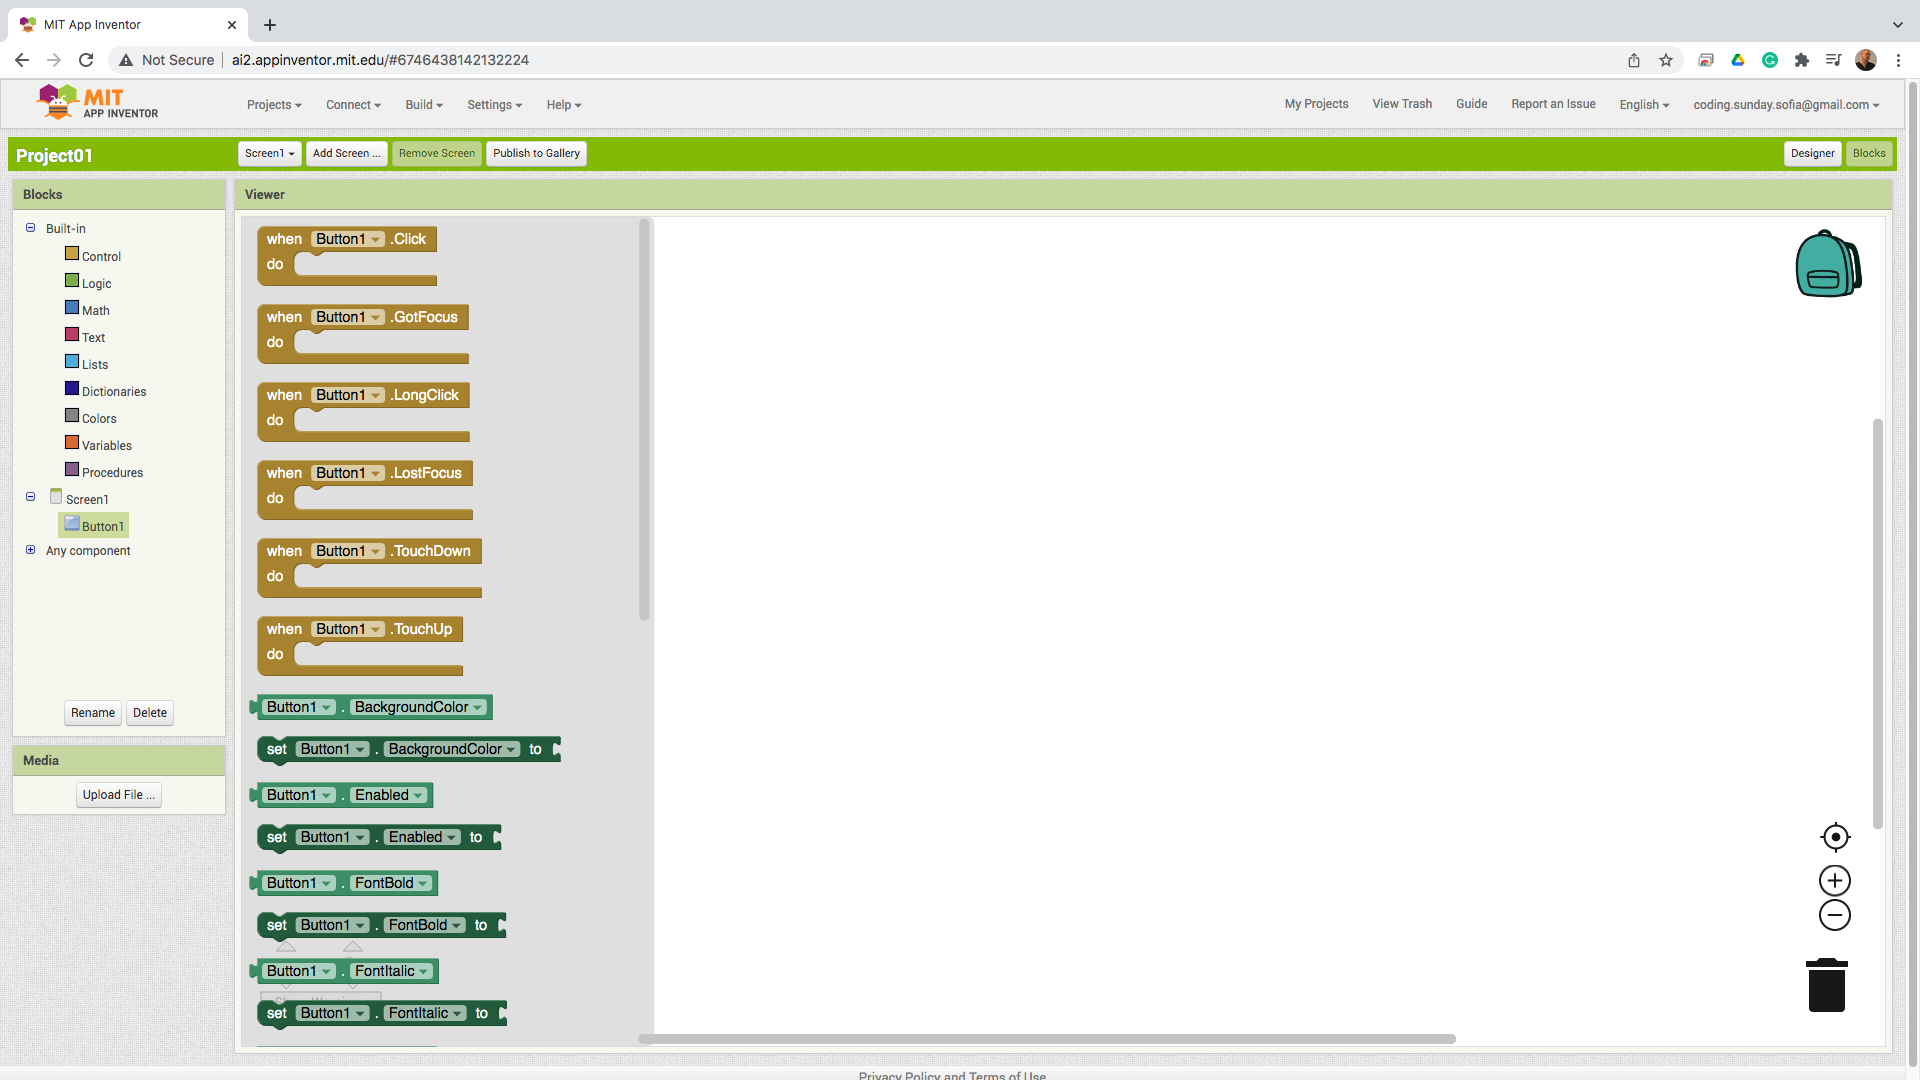
\includegraphics[width=1.0\linewidth,height=0.5\linewidth]{fig010034.png}
  \caption{Списък с инструкции}
\label{fig010034}
\end{figure}

Такова действие би могло да бъде натискането на бутон. От страната на App Inventor, натиснатият бутон генерира събитие (event), за което събитие се избират конкретни действия на програмата (Фиг. \ref{fig010035}). 

\begin{figure}[H]
  \centering
  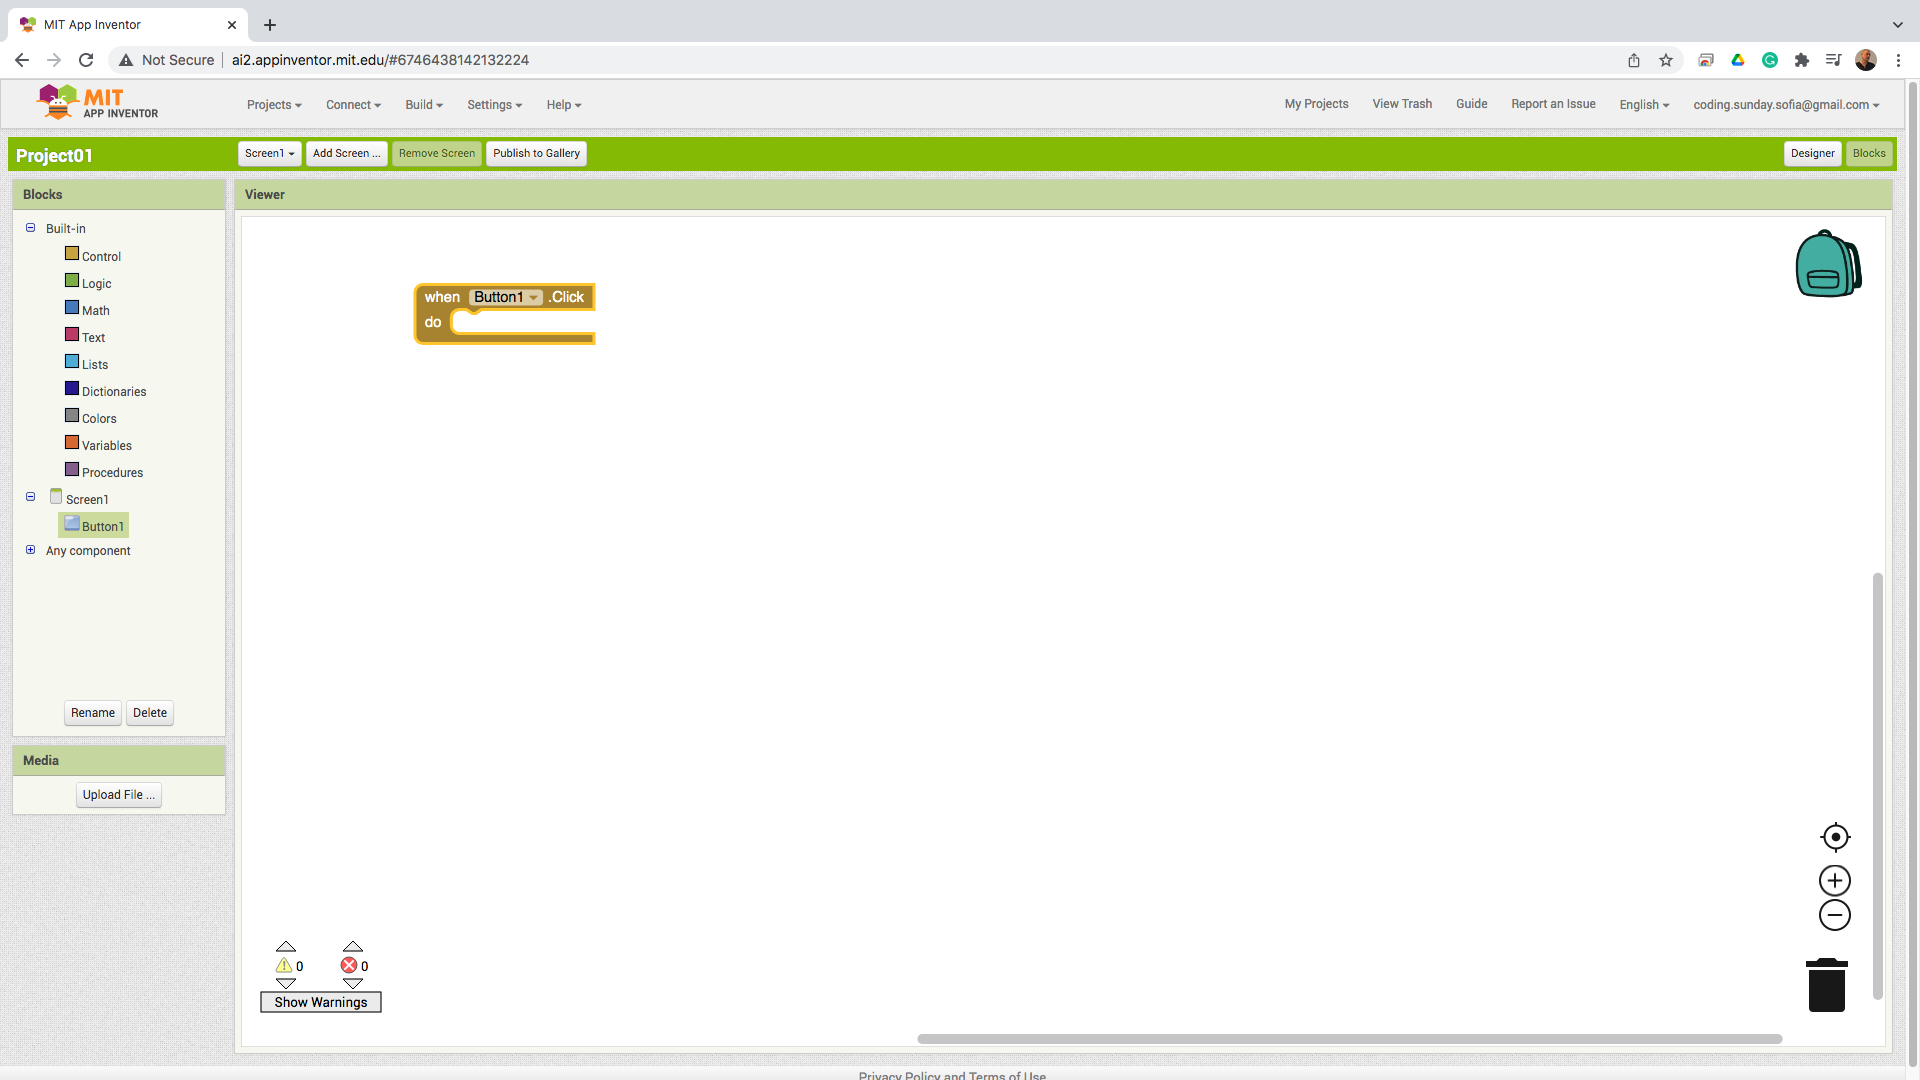
\includegraphics[width=1.0\linewidth,height=0.5\linewidth]{fig010035.png}
  \caption{Избор на събитие за натискане на бутона}
\label{fig010035}
\end{figure}

Събитието за натискане на бутон се визуализира под формата на парче от пъзел, съдържащо слот в който могат да се подредят инструкциите, които трябва да се изпълнят (Фиг. \ref{fig010036}).

\begin{figure}[H]
  \centering
  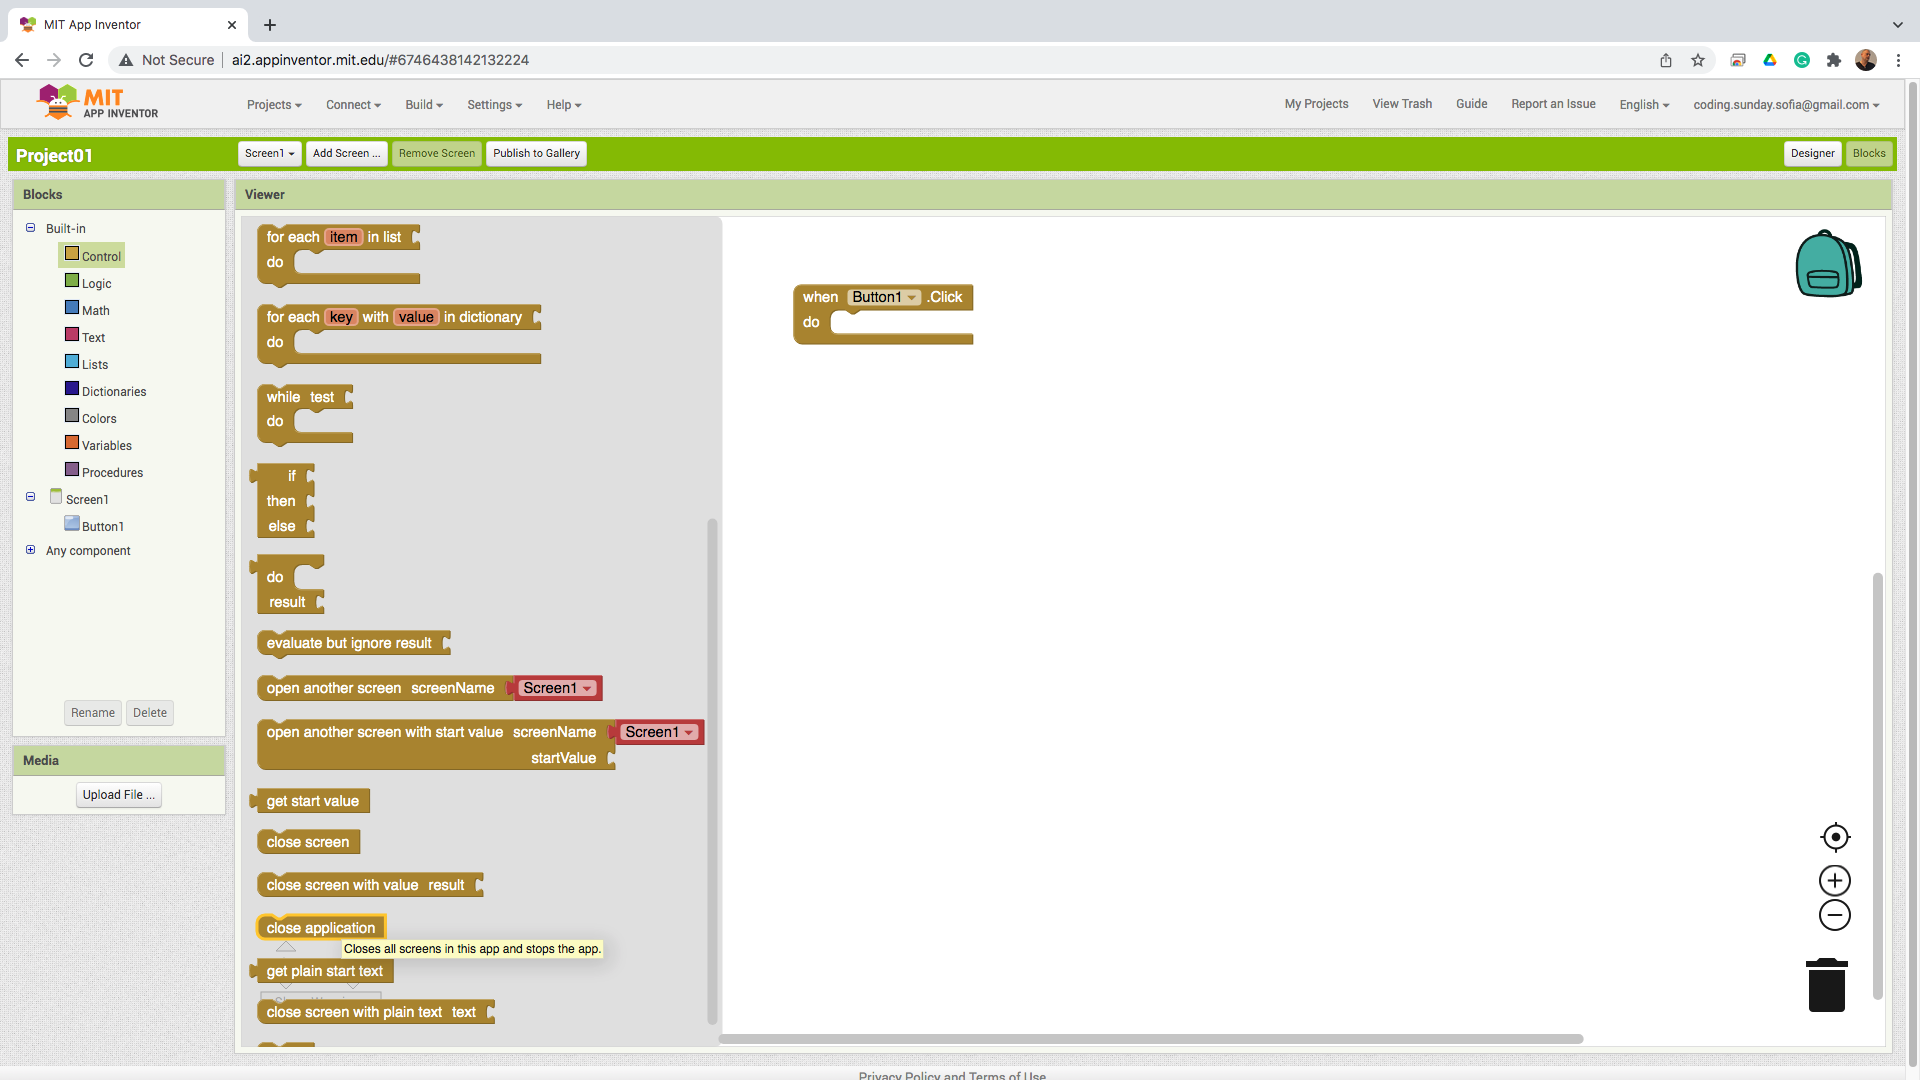
\includegraphics[width=1.0\linewidth,height=0.5\linewidth]{fig010036.png}
  \caption{Избор на действие при натискане на бутона}
\label{fig010036}
\end{figure}

Най-простичкото действие, което може да бъде изпълнено, след натискането на бутона е програмата да бъде спряна и прозорецът на разработваното приложение да бъде затворен (Фиг. \ref{fig010037}).

\begin{figure}[H]
  \centering
  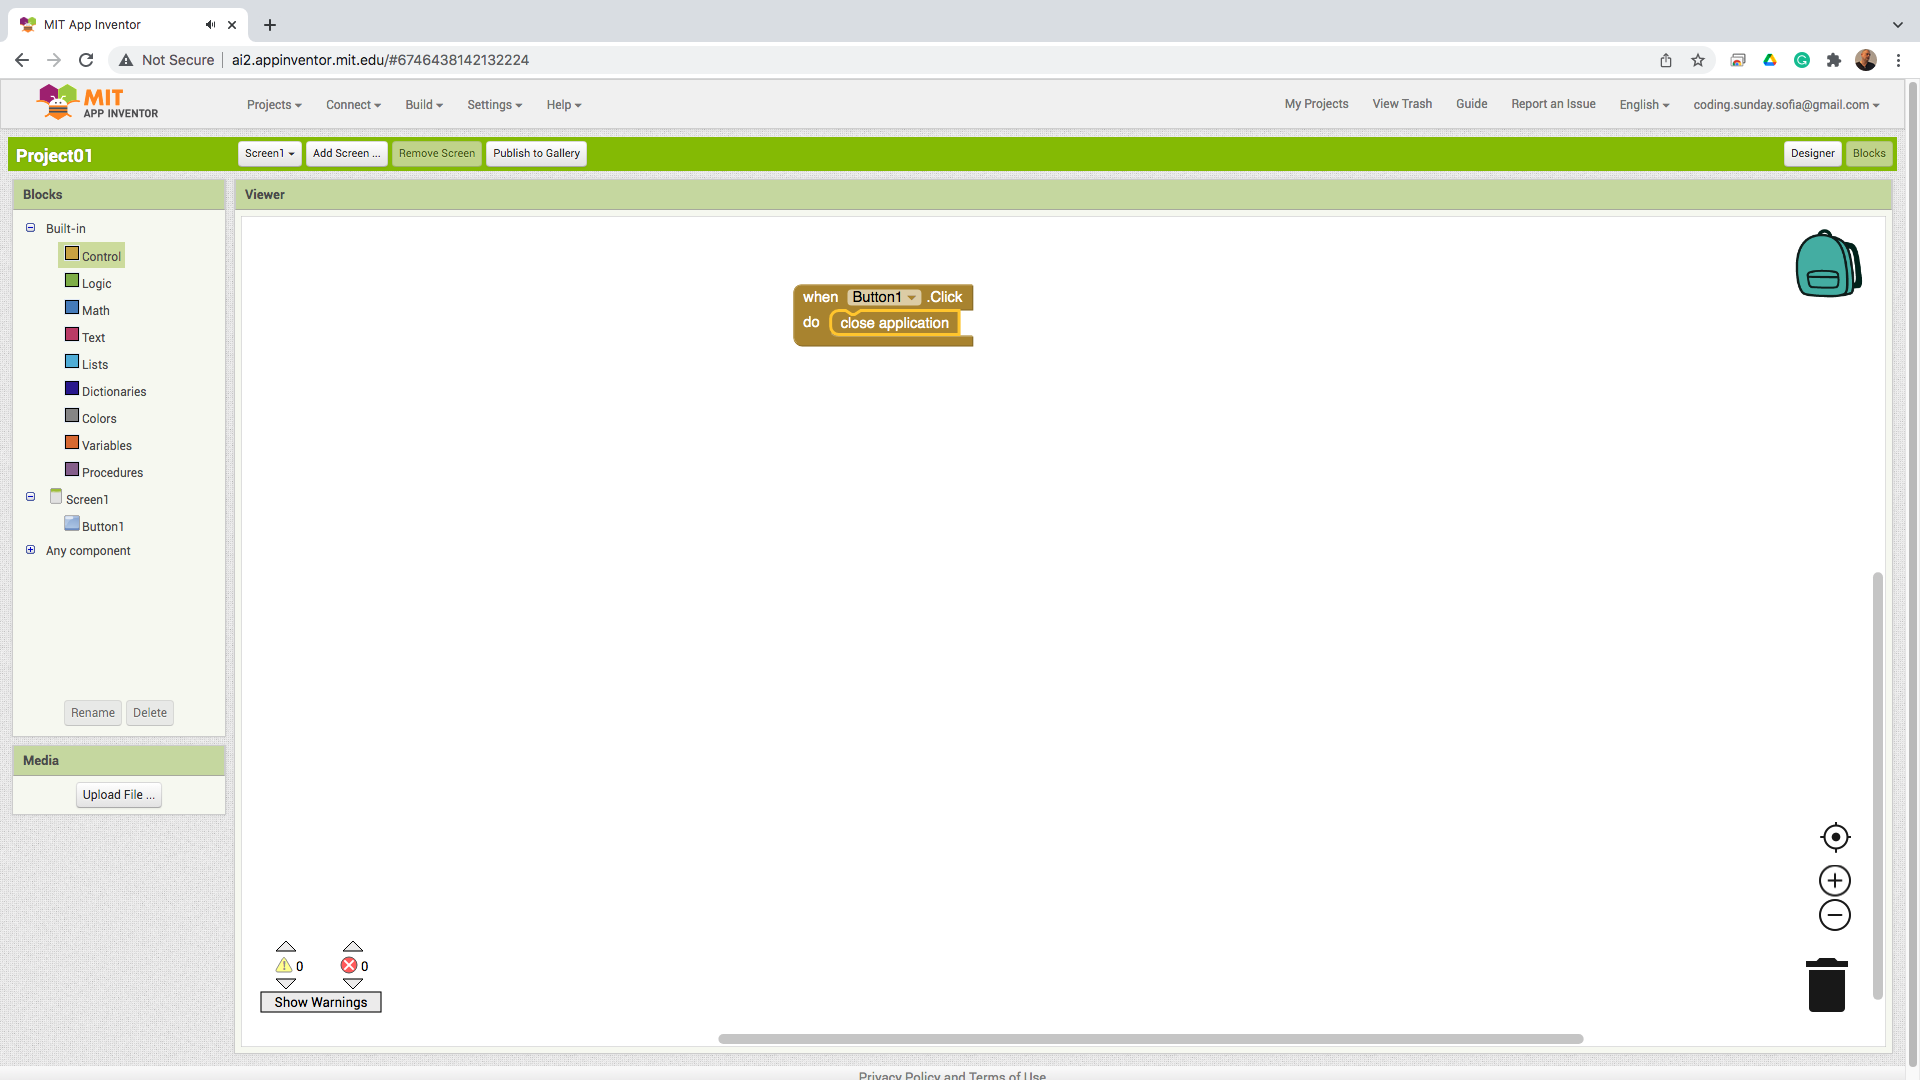
\includegraphics[width=1.0\linewidth,height=0.5\linewidth]{fig010037.png}
  \caption{Затваряне на приложението при натискане на бутона}
\label{fig010037}
\end{figure}

След като графичният програмен интерфейс е оформен и желаните за изпълнение инструкции са подредени, следва компилирането на кода и изграждането на цялостния инсталационен пакет за написаната програма (Фиг. \ref{fig010038}). 

\begin{figure}[H]
  \centering
  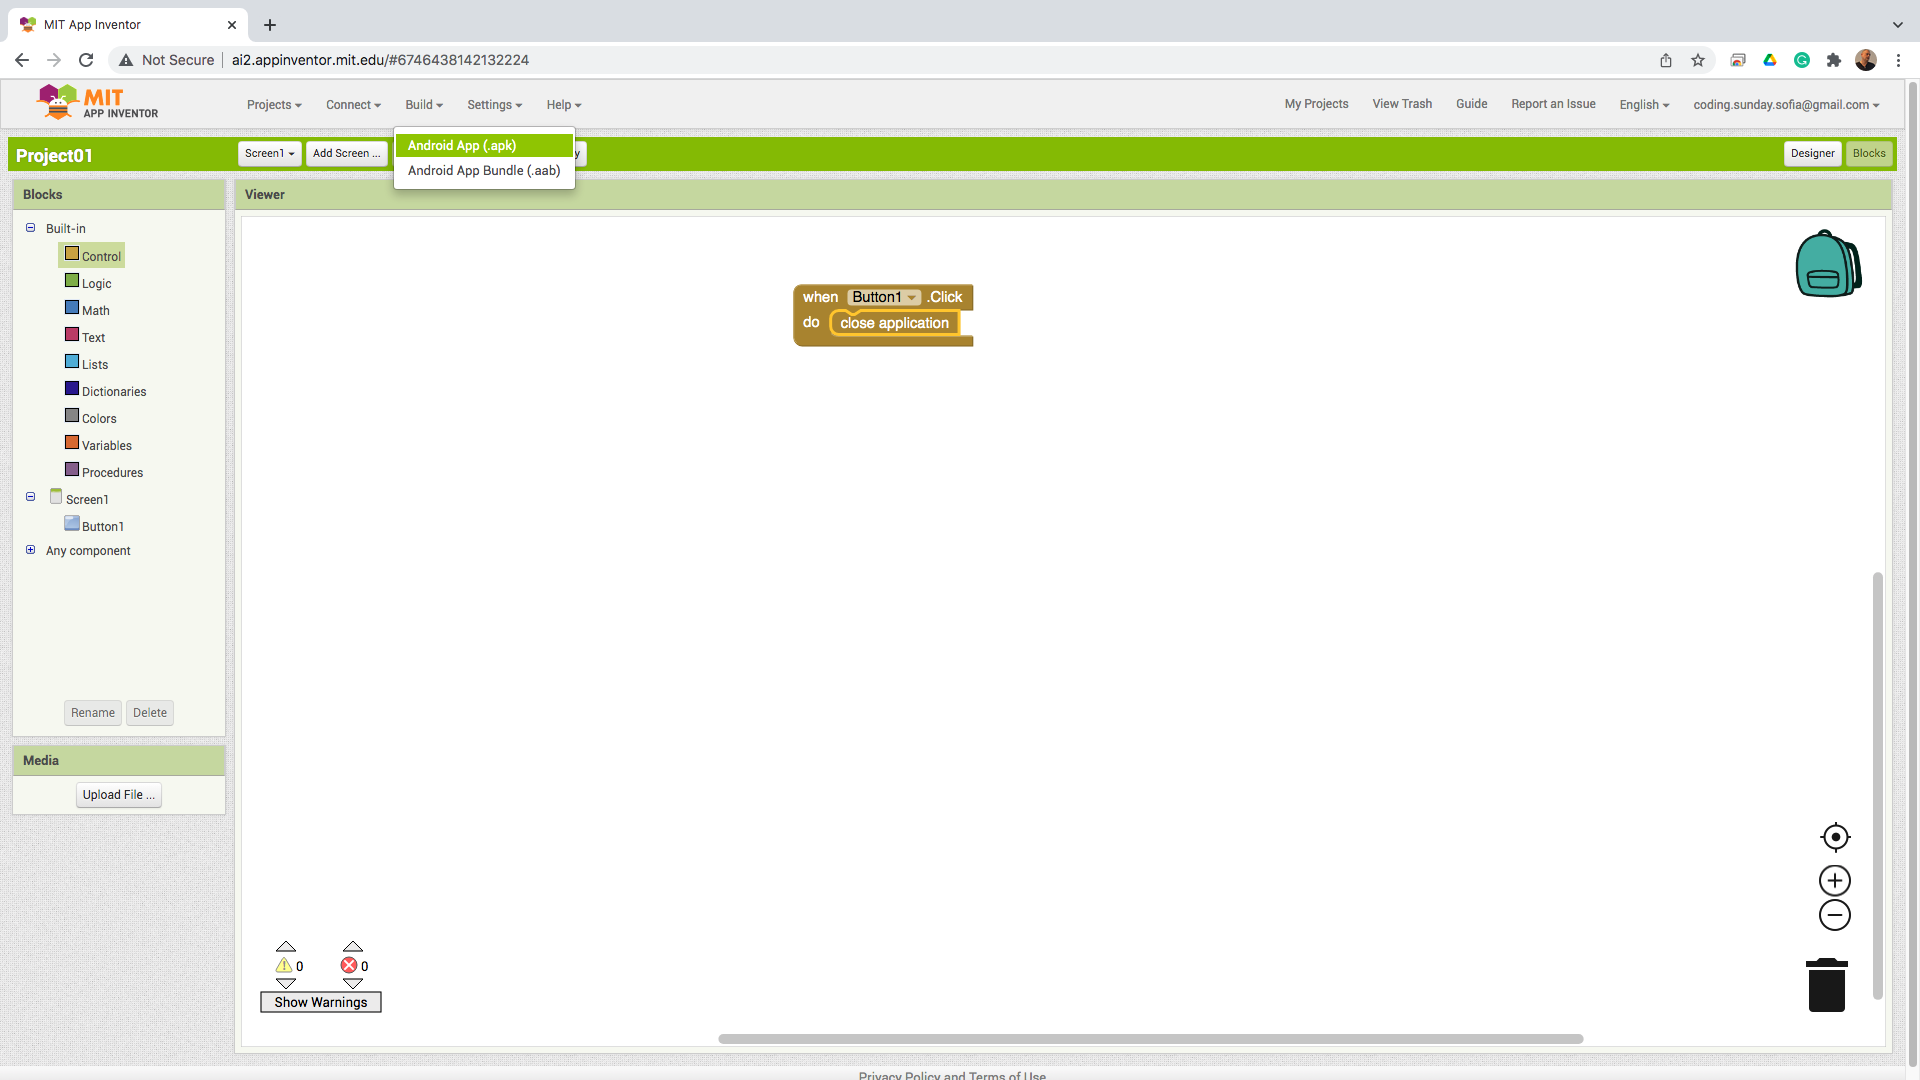
\includegraphics[width=1.0\linewidth,height=0.5\linewidth]{fig010038.png}
  \caption{Меню за изграждане на мобилното приложение}
\label{fig010038}
\end{figure}

Фундаментална разлика между Scratch и App Inventor е, че резултатът от изпълнението на програмните инструкции при Scratch се виждат в самото работно пространство на програмната среда, докато при App Inventor инсталационния пакет на програмата бива компилиран в облачната структура, след това трябва да се изтегли и инсталира на мобилно устройство. Процесът по компилация и изграждане на инсталационния пакет изисква определено изчислително време, визуализирано под формата на прогрес бар (Фиг. \ref{fig010039}).

\begin{figure}[H]
  \centering
  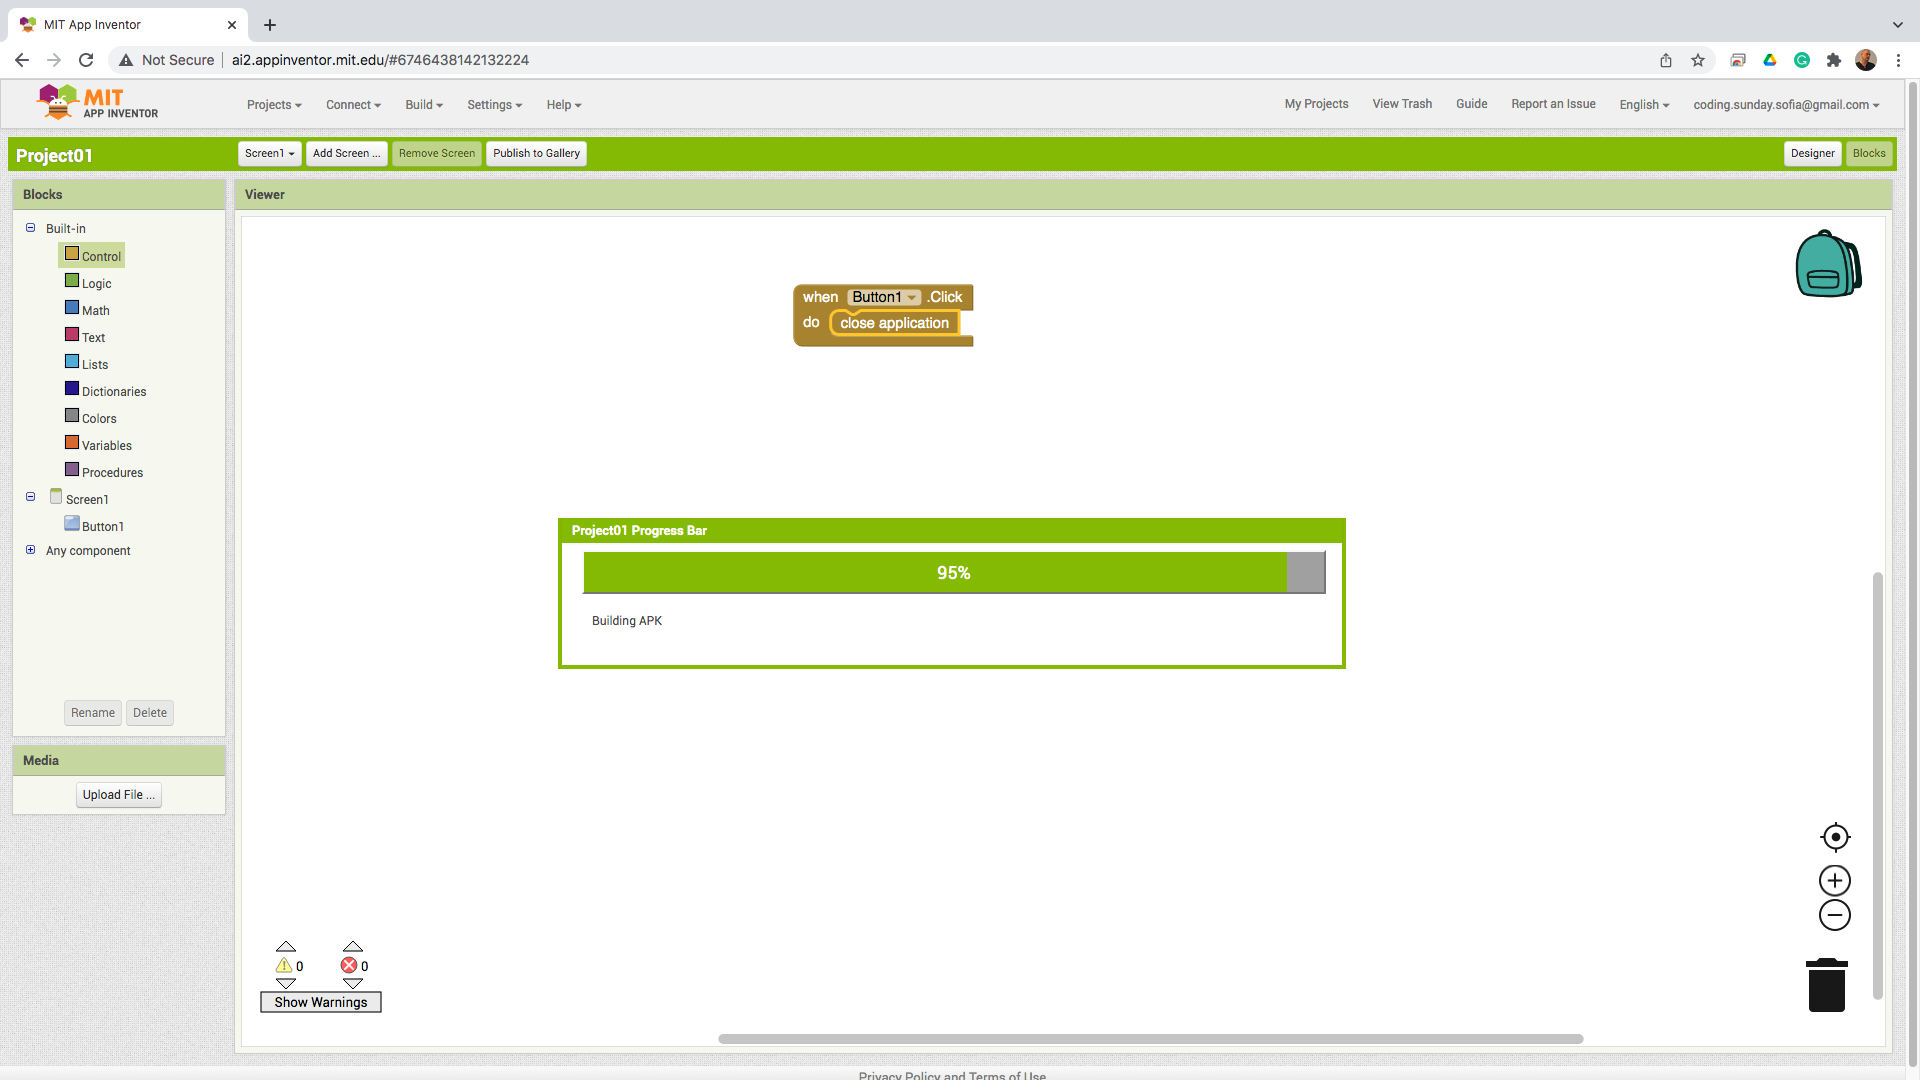
\includegraphics[width=1.0\linewidth,height=0.5\linewidth]{fig010039.png}
  \caption{Прогрес при изграждането на приложението}
\label{fig010039}
\end{figure}

След като проектът е компилиран и инсталационният пакет е създаден, програмната среда предлага QR код (Фиг. \ref{fig010040}), чрез който инсталационния пакет да бъде изтеглен от мобилното устройство (телефон или таблет).

\begin{figure}[H]
  \centering
  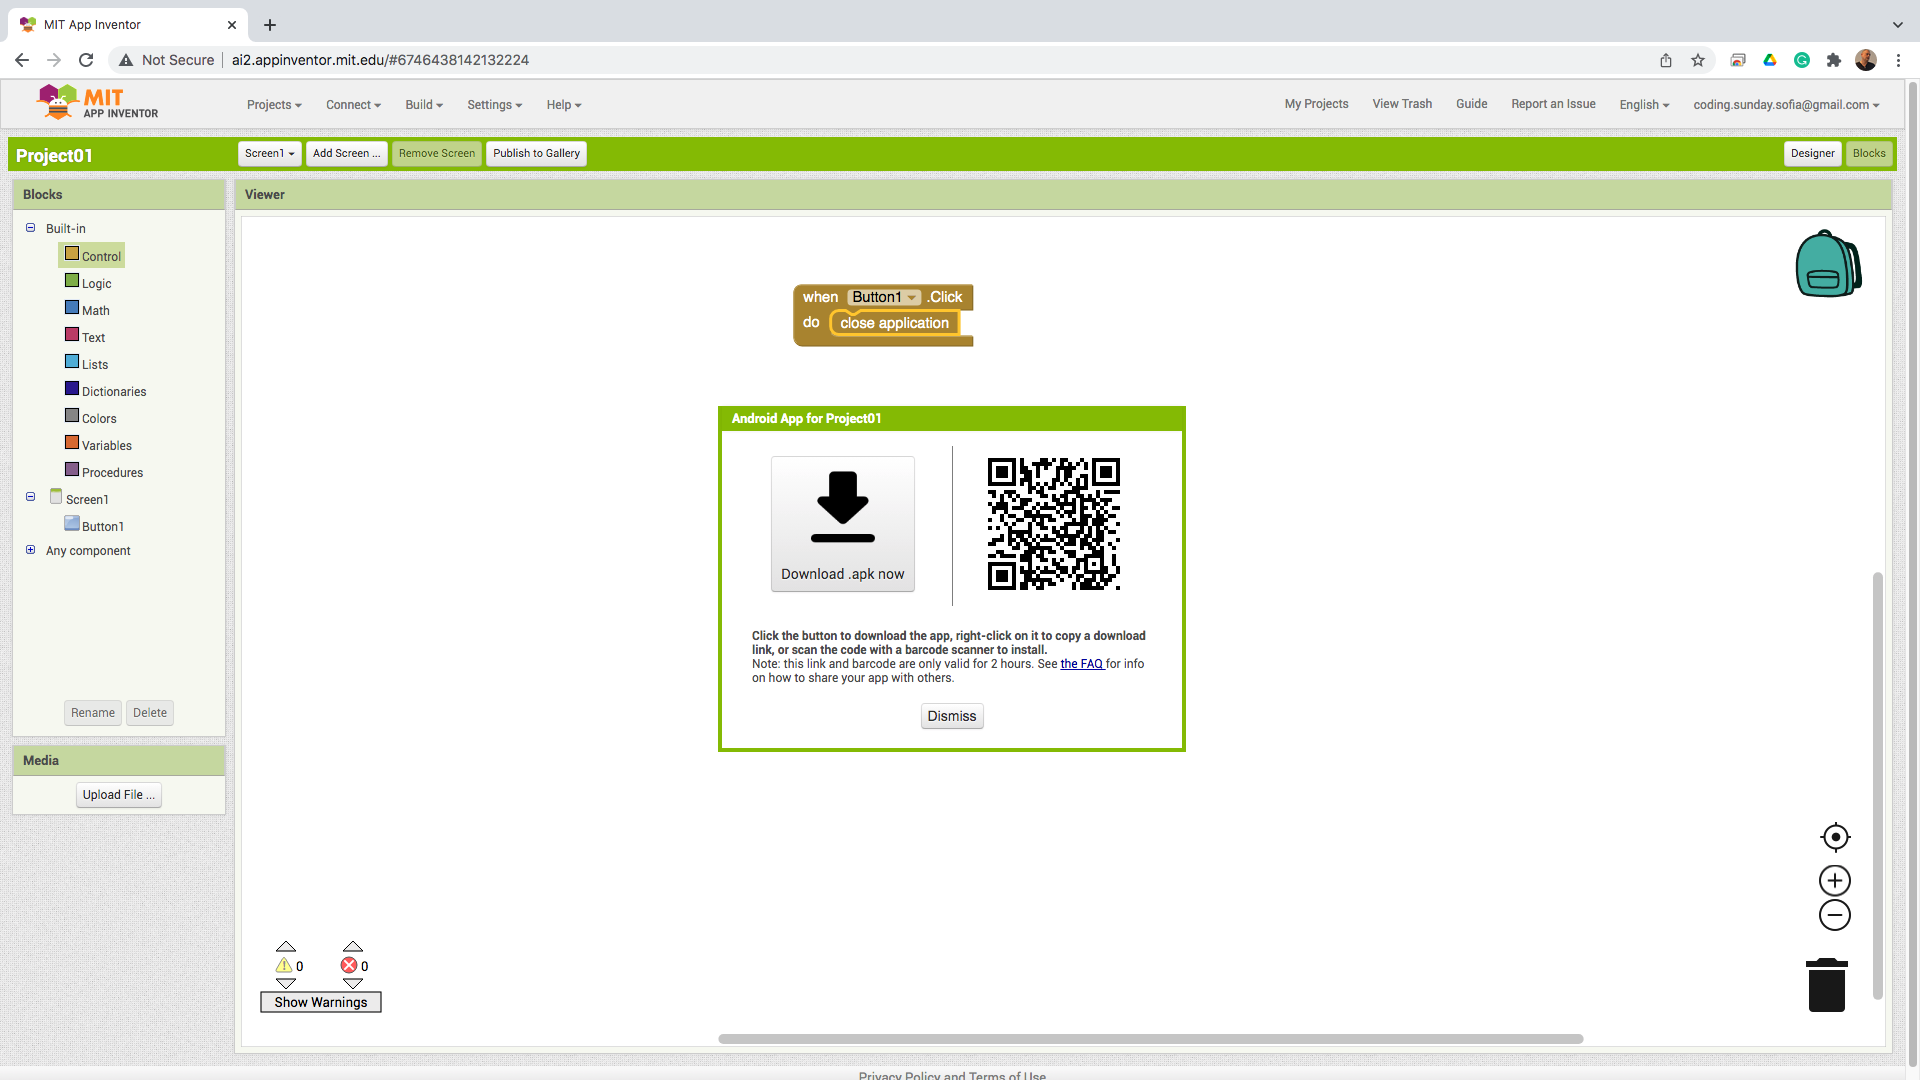
\includegraphics[width=1.0\linewidth,height=0.5\linewidth]{fig010040.png}
  \caption{Код за инсталация на приложението върху мобилно устройство}
\label{fig010040}
\end{figure}

Създателите на програмната среда App Inventor са предвидили възможност за по-бърза и лесна инсталация на написаните програми, чрез специално създадено приложение (MIT AI2 Companion), което да поеме комуникацията с облачната инфраструктура на App Inventor (Фиг. \ref{fig010041}). Приложението е достъпно в Google Play и не изисква никакви специални умения за да бъде инсталирано на личното мобилно устройство. 

\begin{figure}[H]
  \centering
  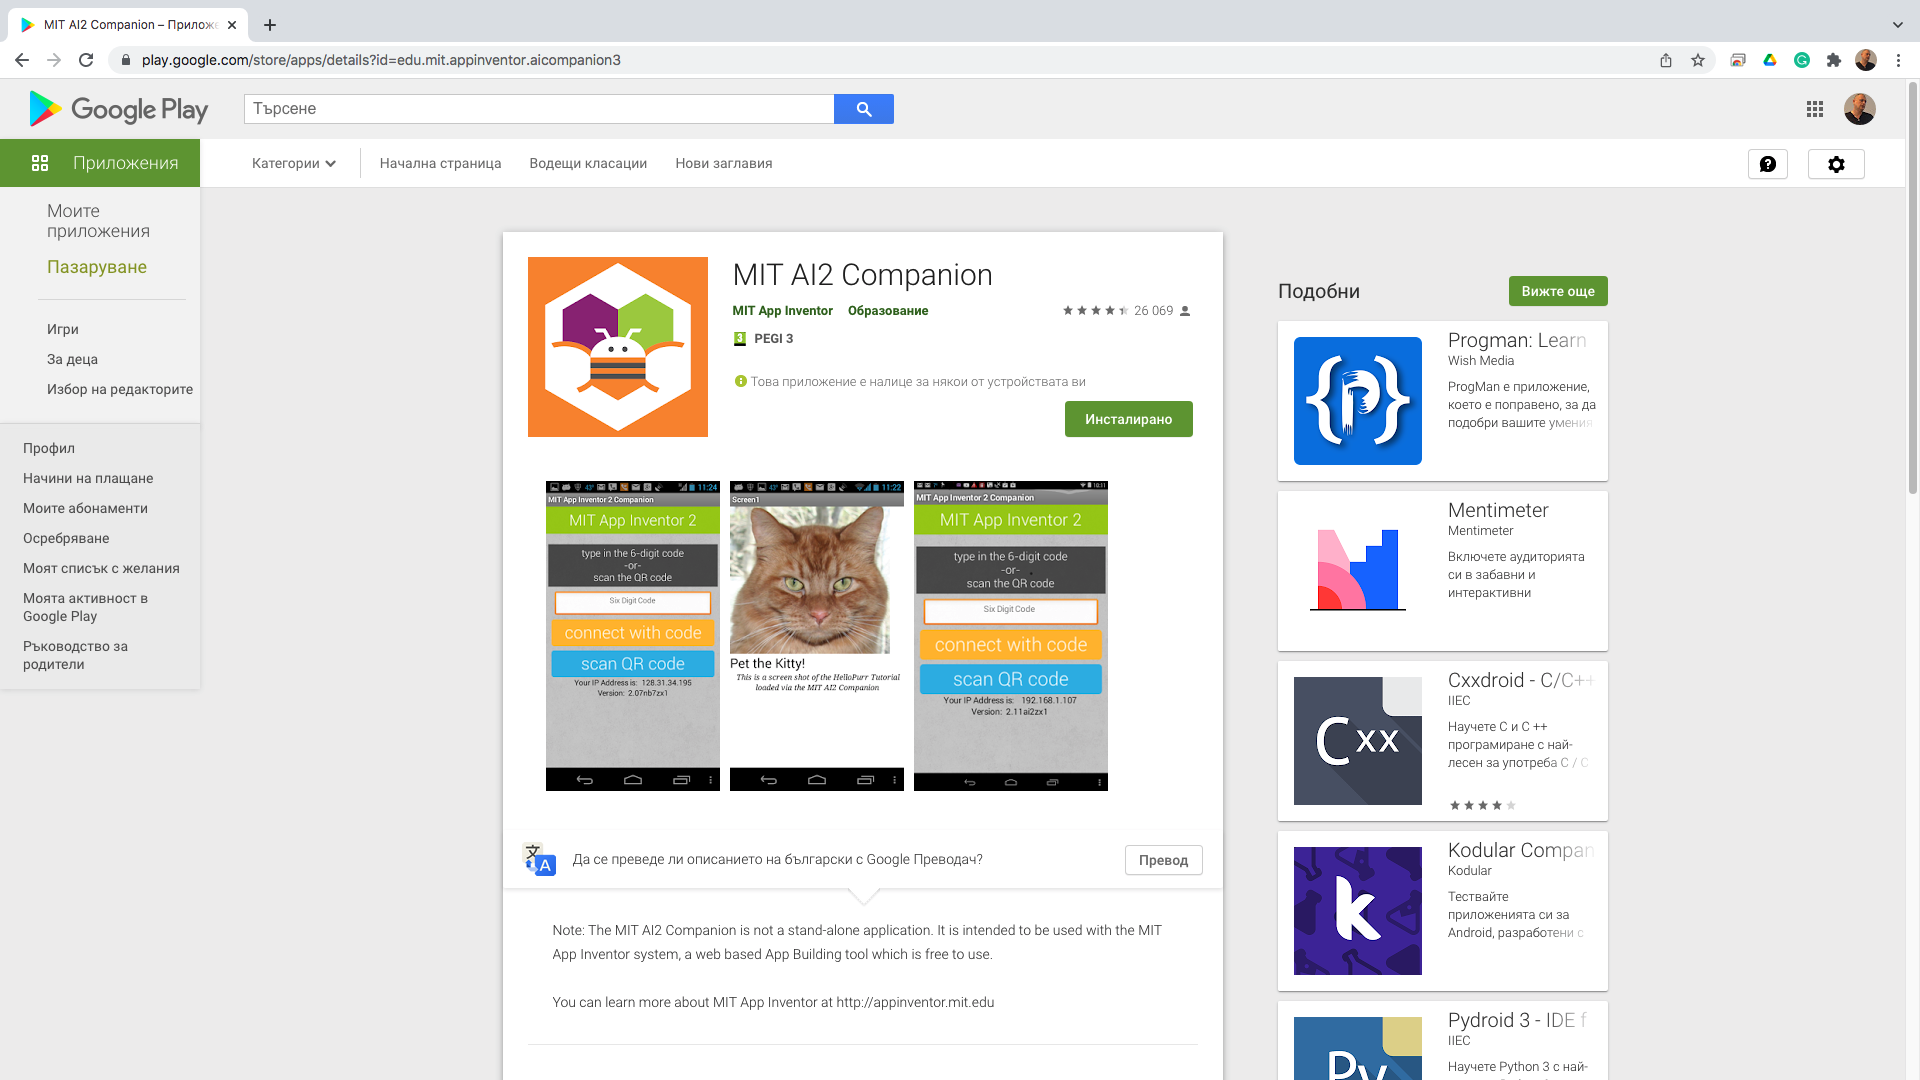
\includegraphics[width=1.0\linewidth,height=0.5\linewidth]{fig010041.png}
  \caption{Мобилно приложение за управление на компилираните проекти}
\label{fig010041}
\end{figure}

Когато се стартира MIT AI2 Companion, приложението дава две възможности за изтегляне на вече написаните програми (Фиг. \ref{fig010042}). Единият вариант е чрез въвеждане на код, а вторият вариант е чрез сканиране на QR код. Сканирането на QR кода е значително по-бързо и по удобно (Фиг. \ref{fig010043}). Тъй като инсталационният пакет представлява изпълним файл, Android операционната система издава предупреждение, че такива файлове могат да бъдат опасни при използването им (Фиг. \ref{fig010044}).

\begin{figure}[H]
  \begin{subfigure}{0.31\textwidth}
  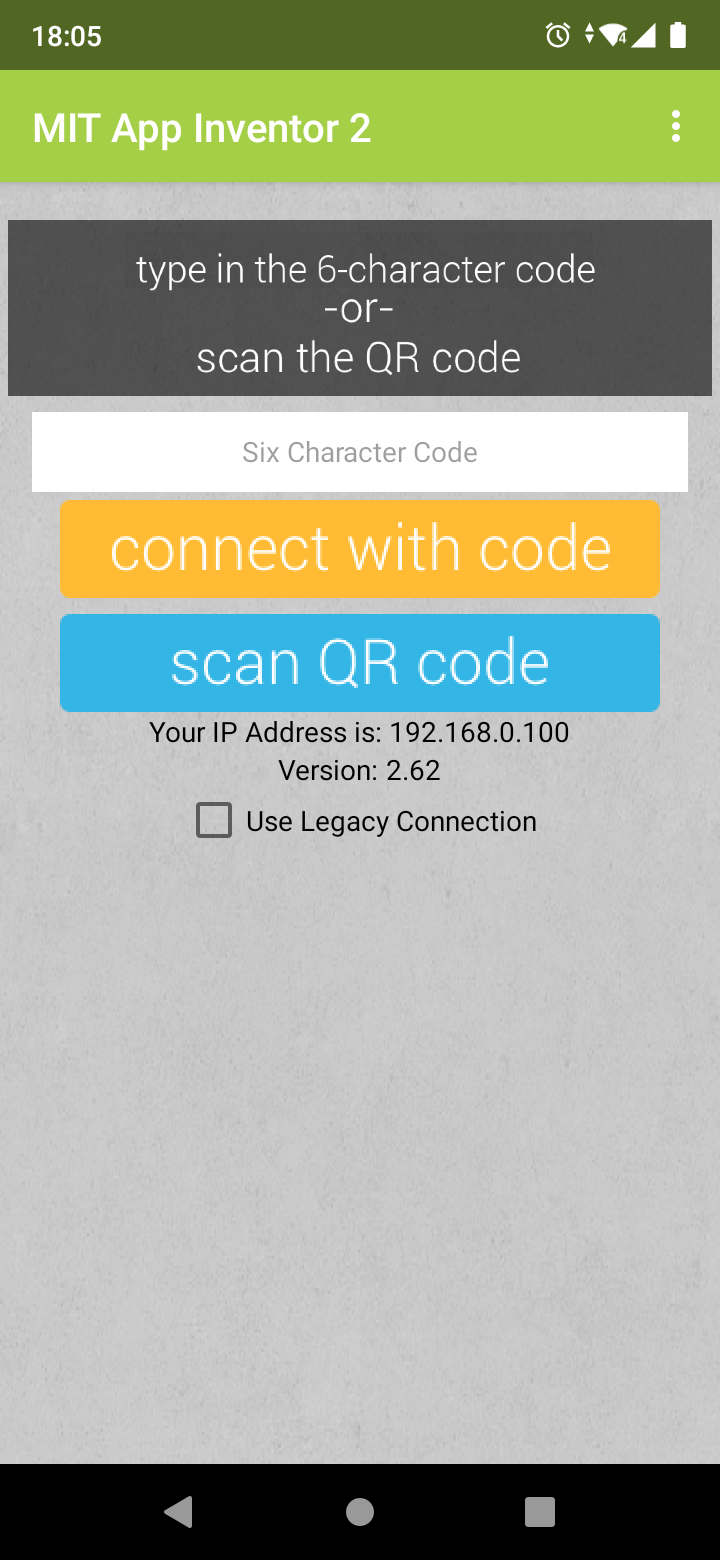
\includegraphics[width=\linewidth]{fig010042.png}
  \subcaption{\tiny Избор на инсталация}
  \label{fig010042}
  \end{subfigure}
  \begin{subfigure}{0.31\textwidth}
  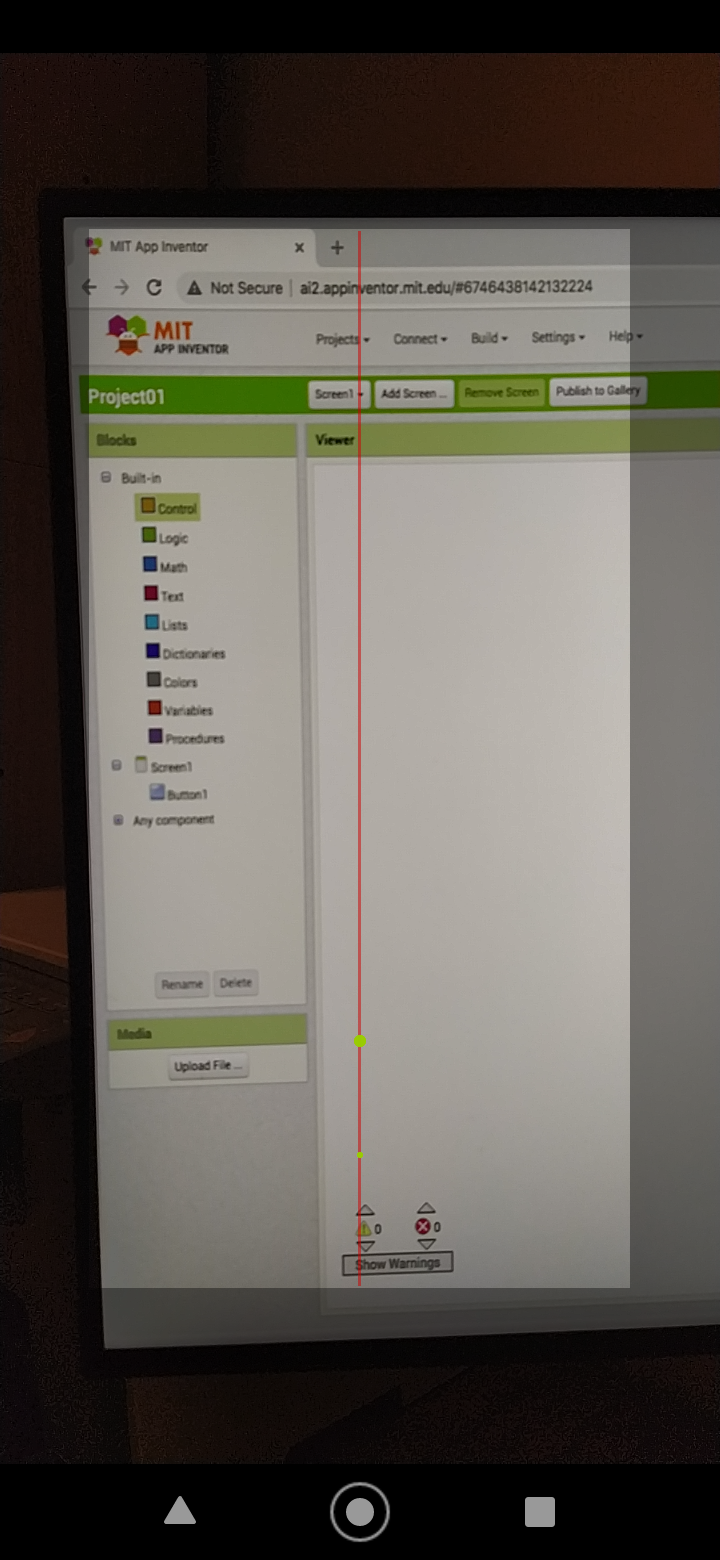
\includegraphics[width=\linewidth]{fig010043.png}
  \subcaption{\tiny Сканиране на код}
  \label{fig010043}
  \end{subfigure}
  \begin{subfigure}{0.31\textwidth}
  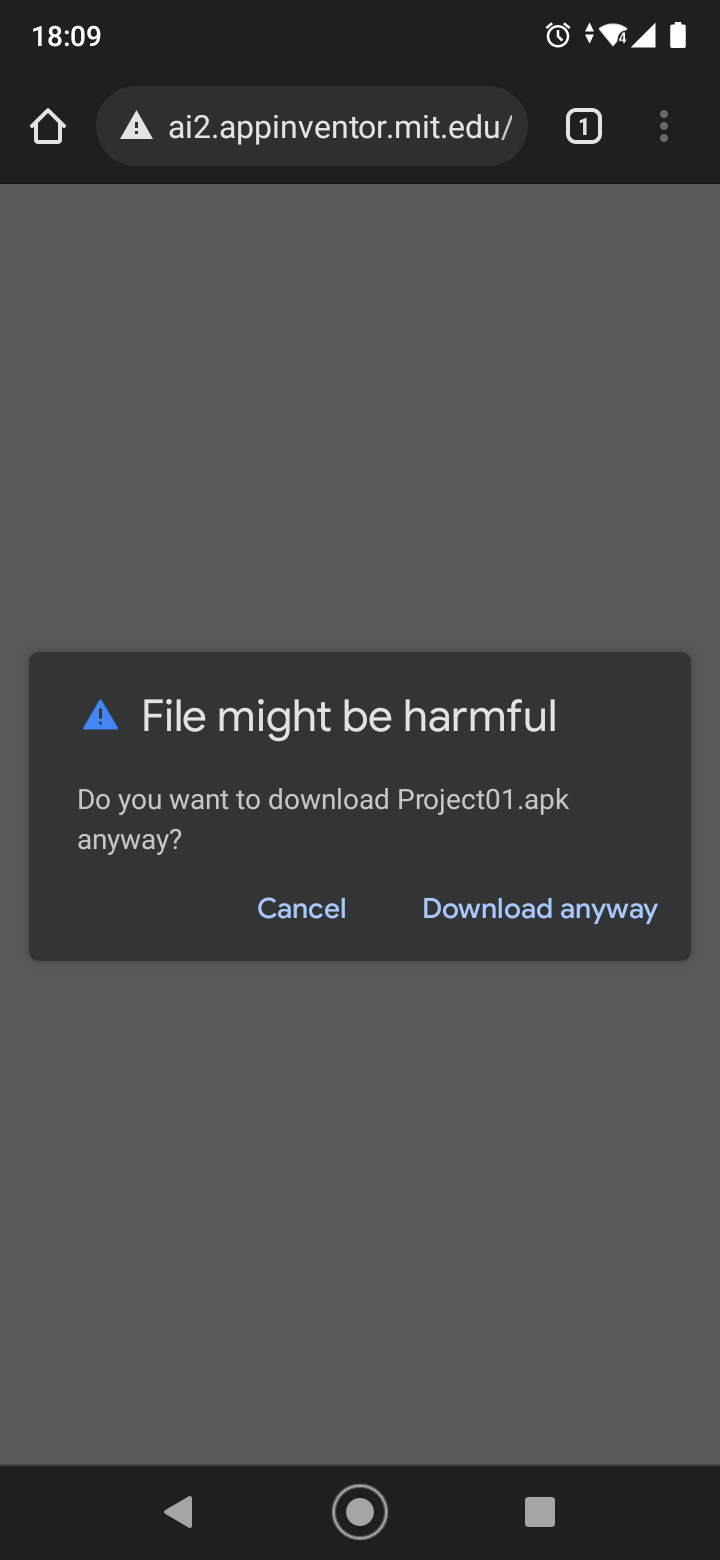
\includegraphics[width=\linewidth]{fig010044.png}
  \subcaption{\tiny Сваляне на файл}
  \label{fig010044}
  \end{subfigure}
  \caption{Инсталация през QR код}
\end{figure}

След като инсталационният пакет бива свален, операционната система издава съобщение за успешно извършена операция по запис на инсталатора (Фиг. \ref{fig010045}). Потребителят трябва да избере инсталационния пакет и да го активира. Това води до запитване дали действително желае да инсталира програмата, съдържана в сваления файл (Фиг. \ref{fig010046}). Въпреки, че ние сме наясно как точно е бил създаден инсталационният файл, операционната система го възприема, като програма създадена от непроверен разработчик. Поради тази причина, повторно задава въпрос на потребителя дали желае да направи инсталацията (Фиг. \ref{fig010047}). 

\begin{figure}[H]
  \begin{subfigure}{0.31\textwidth}
  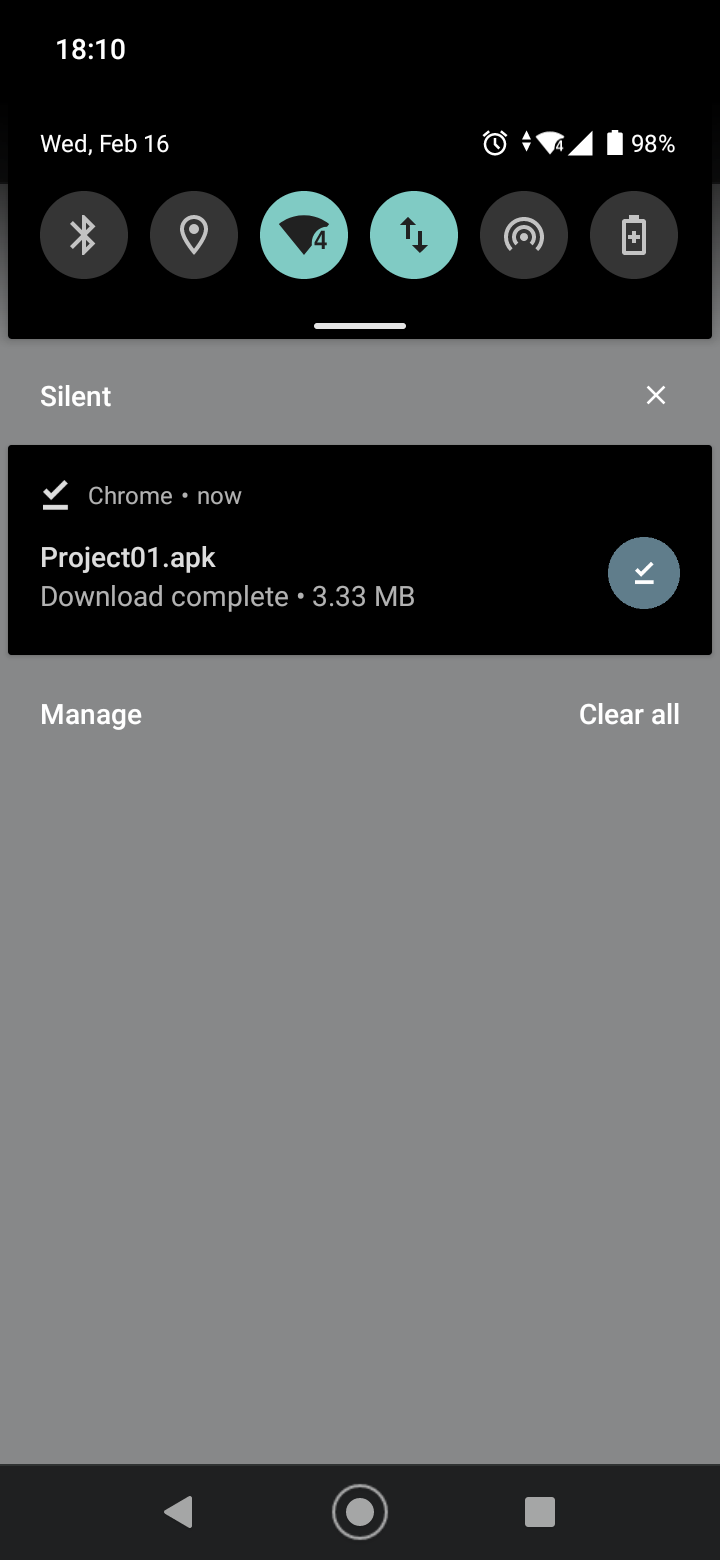
\includegraphics[width=\linewidth]{fig010045.png}
  \subcaption{\tiny Свален файл}
  \label{fig010045}
  \end{subfigure}
  \begin{subfigure}{0.31\textwidth}
  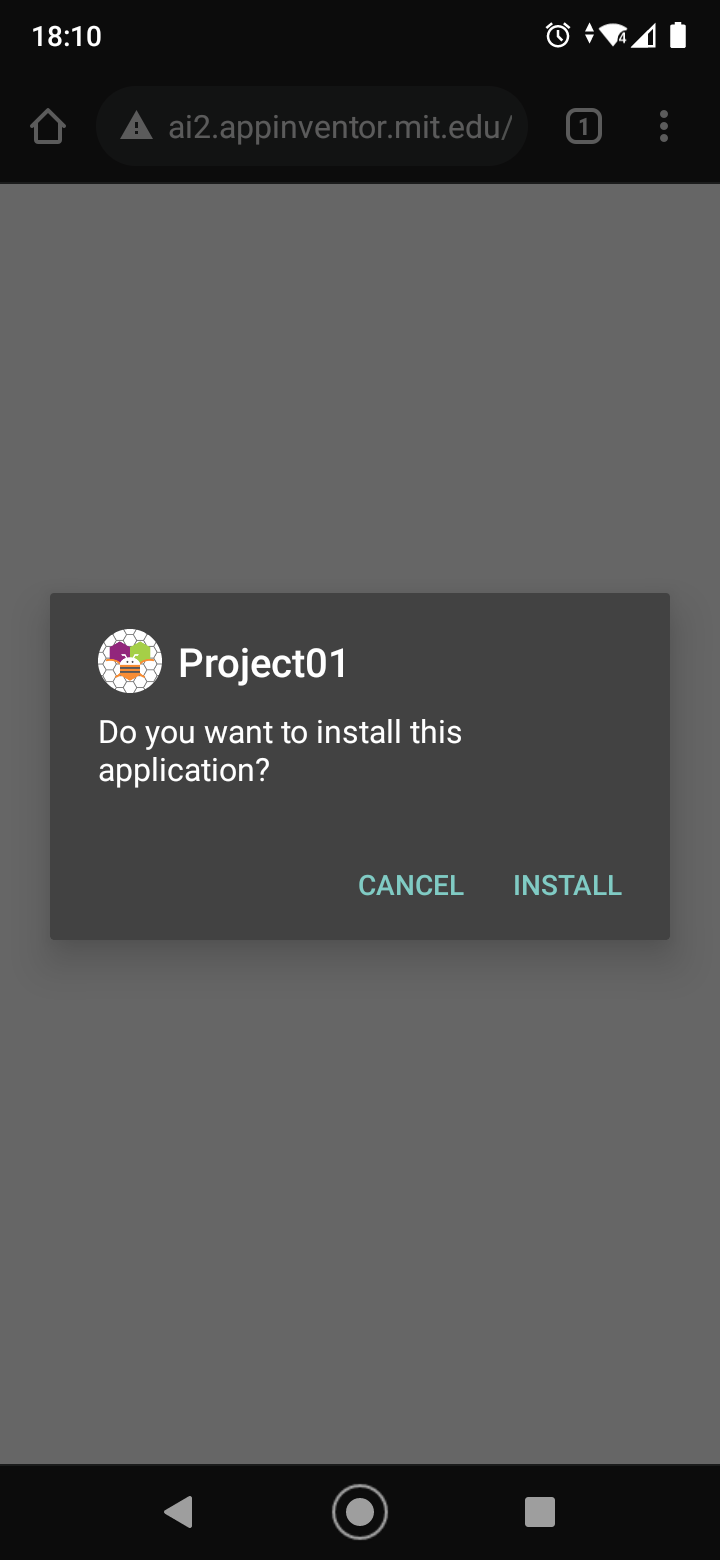
\includegraphics[width=\linewidth]{fig010046.png}
  \subcaption{\tiny Избор за инсталиране}
  \label{fig010046}
  \end{subfigure}
  \begin{subfigure}{0.31\textwidth}
  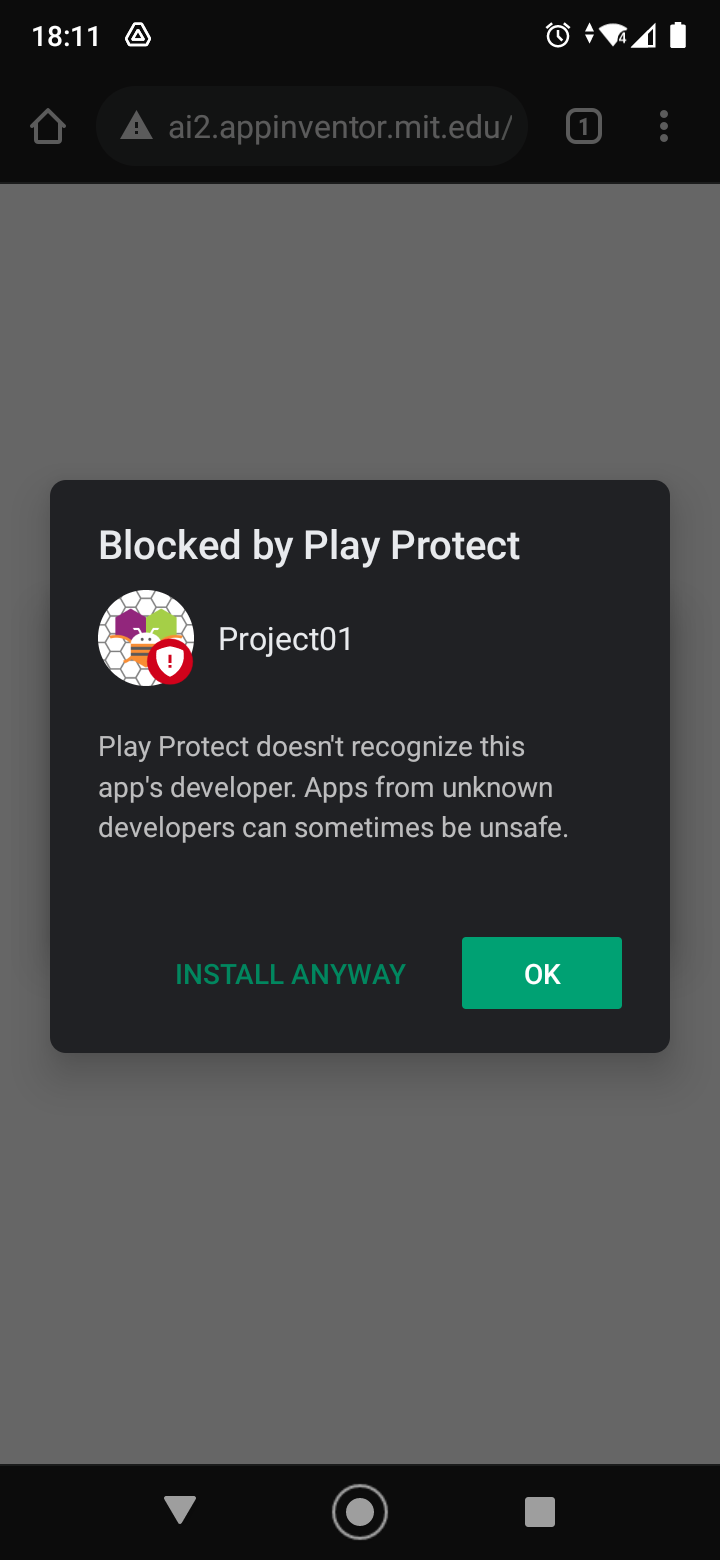
\includegraphics[width=\linewidth]{fig010047.png}
  \subcaption{\tiny Потвърждение за инсталиране}
  \label{fig010047}
  \end{subfigure}
  \caption{Инсталация върху мобилното устройство}
\end{figure}

Избира се „Install Anyway“ и написаната програма бива инсталирана върху мобилното устройство. Процесът по инсталацията завършва с подканящ прозорец за стартиране на новоинсталираната програма (Фиг. \ref{fig010048}). За да се провери работата на написания код е достатъчно да бъде натиснат визуализирания бутон в горния ляв ъгъл (Фиг. \ref{fig010049}). Резултатът от това действие е затваряне на прозореца и визуализиране на виртуалния тапет (Фиг. \ref{fig010049}).

\begin{figure}[H]
  \begin{subfigure}{0.31\textwidth}
  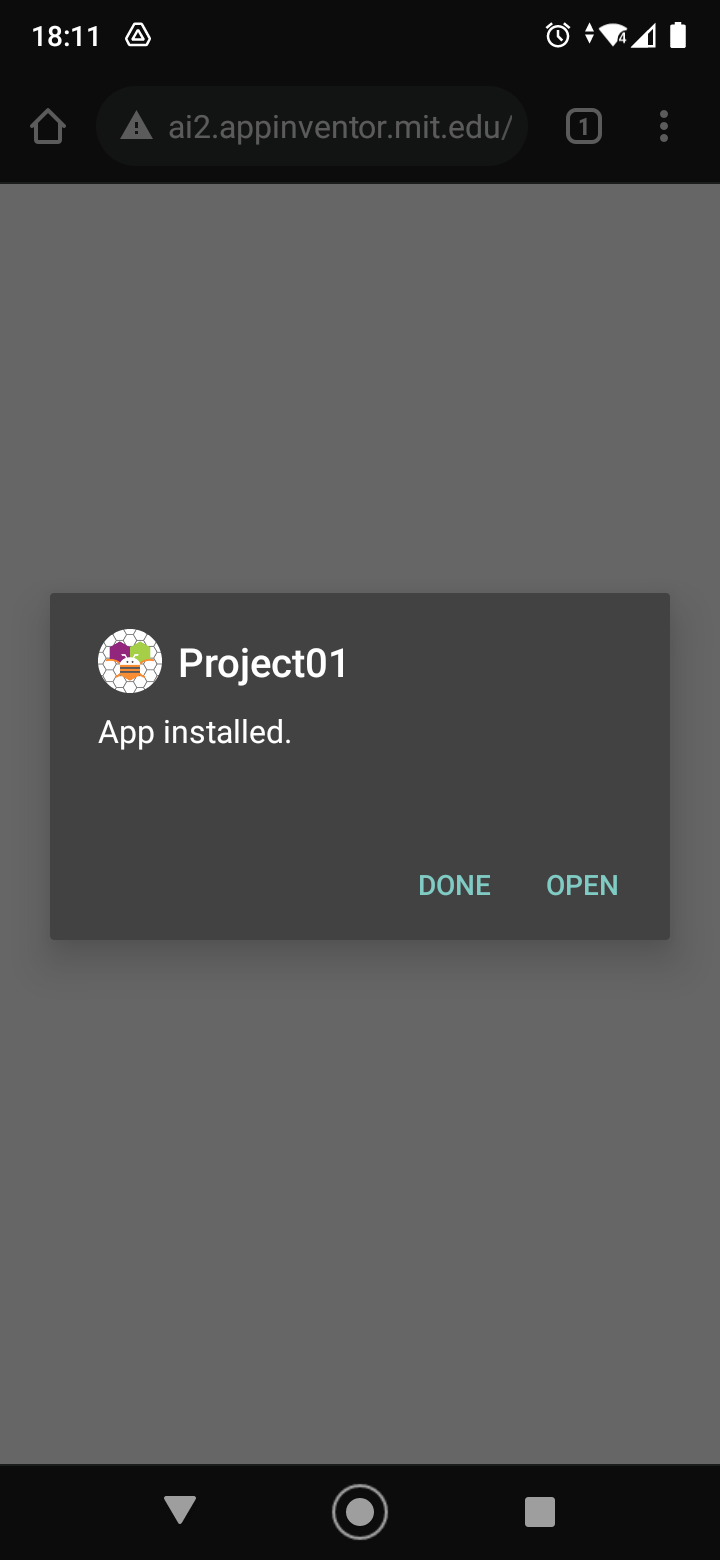
\includegraphics[width=\linewidth]{fig010048.png}
  \subcaption{\tiny Стартиране}
  \label{fig010048}
  \end{subfigure}
  \begin{subfigure}{0.31\textwidth}
  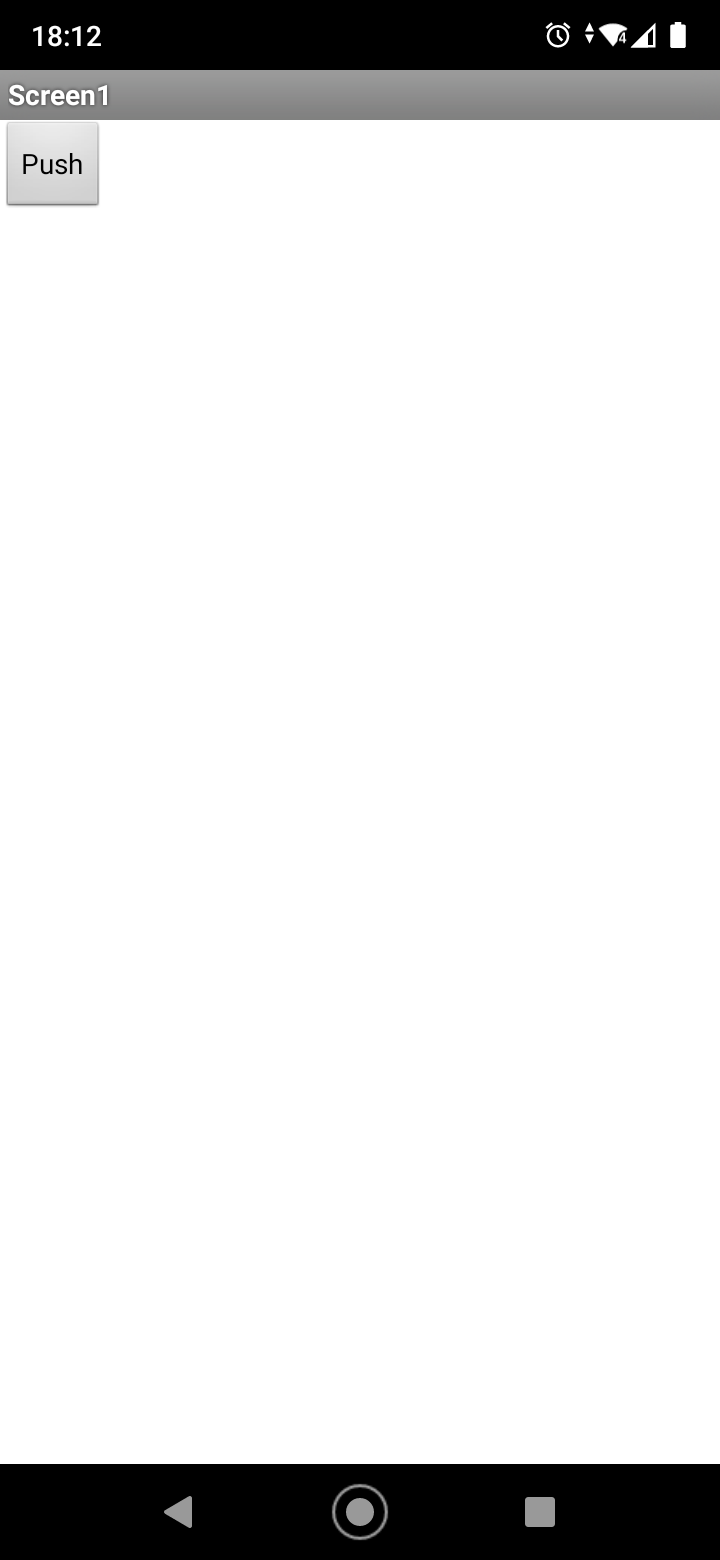
\includegraphics[width=\linewidth]{fig010049.png}
  \subcaption{\tiny Избор на бутона}
  \label{fig010049}
  \end{subfigure}
  \begin{subfigure}{0.31\textwidth}
  \includegraphics[width=\linewidth]{fig010050.png}
  \subcaption{\tiny Затворено приложение}
  \label{fig010050}
  \end{subfigure}
  \caption{Работа с приложението}
\end{figure}

При App Inventor най-очарователната част е, че разработените програми стават налични на мобилните устройства и човекът, който ги създава може да показва своята работа, дори когато не е пред компютър или не разполага с Интернет свързаност. 

\newpage
\chapter{Програмни конструкции}

Компютърните програми са съставени от стриктна последователност инструкции. Такива последователности се наричат алгоритъм. Ние хората всеки ден изпълняваме различни алгоритми, като част от нашето ежедневие. Да се приготвим и да отидем на училище е един алгоритъм. Събуждаме се, ставаме, обличаме се, правим си сутрешния тоалет, закусваме, излизаме от вкъщи, придвижваме се до училище. Много ярък пример за алгоритъм са рецептите за готвене. В една рецепта има начални продукти, след това точни инструкции как продуктите са се обработят и смесят, като има ясна представа какъв трябва да бъде крайният резултат. При компютърните програми има основен набор от инструкции, които съставляват изразните средства на съответния програмен език. Чарът на блоковите езици е, че този основен набор от инструкции е представен визуално, под формата на цветни блокчета. Подредбата на цветните блокчета в строго определена последователност води до създаването на малки компютърни програми. 

В случая на Scratch, програмата има ясно определена стартова точка и ясно определена финална точка. При App Inventor подходът е малко по-различен. Там последователността от инструкции, съставляващи писаната програма, се въвежда в малки фрагменти, наречени събития. Събитията възникват при различни действия от страна на потребителя или операционната система. При Scratch говорим за последователно програмиране, а при App Inventor говорим за събитийно програмиране. Основните програмни конструкции в двете програмни среди до голяма степен са идентични, но има и някои съществени разлики. За да можем да пишем ефективни и надеждни програми е важно добре да познаваме изразните средства на програмните среди с които работим. 

\section{Изразни средства в Scratch}

Базовите градивни блокчета в Scratch са организирани в цветни групи (Фиг. \ref{fig020001}). Тази организация помага за по-бързо ориентиране и по-ефективна употреба на различните блокчета. 

\begin{figure}[H]
  \centering
  \includegraphics[width=1.0\linewidth,height=0.5\linewidth]{fig020001.png}
  \caption{Групиране на инструкциите}
\label{fig020001}
\end{figure}

Най-важното блокче в програмата е блокчето, което дава старт за изпълнение на инструкциите, които са подредени под него. Това блокче има зелен флаг (Фиг. \ref{fig020002}) и определя какво ще последва след стартирането на програмата.

\begin{figure}[H]
  \centering
  \includegraphics[width=1.0\linewidth,height=0.5\linewidth]{fig020002.png}
  \caption{Начална точка на програмата}
\label{fig020002}
\end{figure}

Блокчето за старт на програмата се намира в светло оранжевата група, която е предназначена да реагира на събития от страна на потребителя. Точният момент в който потребителят иска програмата да започне своето изпълнение е неопределен във времето и поради тази причина Scratch трябва да улови събитие, предизвикано от самия потребител. 

Второто по важност блокче служи за край на програмата (Фиг. \ref{fig020003}). То се намира в тъмно оранжевата група и има за задача да спре всички процеси, извършващи се по време на изпълнението на самата програма.

\begin{figure}[H]
  \centering
  \includegraphics[width=1.0\linewidth,height=0.5\linewidth]{fig020003.png}
  \caption{Крайна точка на програмата}
\label{fig020003}
\end{figure}

Тъмно оранжевата група съдържа блокчета за контрол на изпълнението. Тези блокчета позволяват програмата да поема по различни пътища, както и група от действия да се повтарят многократно. 

В Scratch блокчетата инструкции основно контролират картинки, наречени спрайтове (sprites). За разлика от обикновеното компютърно изображение, спрайтът е графичен обект, който съдържа множество кадри, показващи изображението на героя в различни конфигурации. Всяка нова програма в Scratch започва с един спрайт, на оранжевата котка, разположена на координати (x=0,y=0). Работното пространство е двуизмерна координатна система с център (0,0). 

\begin{figure}[H]
  \centering
  \includegraphics[width=1.0\linewidth,height=0.5\linewidth]{fig020004.png}
  \caption{Завършване веднага след започване}
\label{fig020004}
\end{figure}

Ако бъдат съединени, блокчетата за начало и за край (Фиг. \ref{fig020004}), то програмата не изпълнява нищо. Практически, тази програма приключва веднага след като е започнала. Програма, която не прави нищо е напълно безсмислена. За да започне нещо да се случва се използват блокчетата в синята група. Първото блокче инструктира котето да се премести 10 стъпки, като броя стъпки може да бъде променени, чрез изписване на друго число във вътрешността на блокчето (Фиг. \ref{fig020005}).

\begin{figure}[H]
  \centering
  \includegraphics[width=1.0\linewidth,height=0.5\linewidth]{fig020005.png}
  \caption{Преместване на героя}
\label{fig020005}
\end{figure}

Следващият блок в групата инструктира героя да се завърти на определено число градуси, по часовниковата стрелка, спрямо собствения си център (Фиг. \ref{fig020006}).

\begin{figure}[H]
  \centering
  \includegraphics[width=1.0\linewidth,height=0.5\linewidth]{fig020006.png}
  \caption{Завъртане по часовниковата стрелка}
\label{fig020006}
\end{figure}

Аналогично, със следващото блокче в групата, завъртането може да се изпълни и в посока обратна на часовниковата стрелка (Фиг. \ref{fig020007}).

\begin{figure}[H]
  \centering
  \includegraphics[width=1.0\linewidth,height=0.5\linewidth]{fig020007.png}
  \caption{Завъртане обратно на часовниковата стрелка}
\label{fig020007}
\end{figure}

Следващия блок в групата дава възможност героят да се премести на случайни координати или на координати посочени с мишката (Фиг. \ref{fig020008}).

\begin{figure}[H]
  \centering
  \includegraphics[width=1.0\linewidth,height=0.5\linewidth]{fig020008.png}
  \caption{Преместване на случайна позиция}
\label{fig020008}
\end{figure}

Движението на героя може да бъде зададено и чрез абсолютни координати с блокче, позволяващо да се впишат числа за абцисната и ординатната ос (Фиг. \ref{fig020009}).

\begin{figure}[H]
  \centering
  \includegraphics[width=1.0\linewidth,height=0.5\linewidth]{fig020009.png}
  \caption{Преместване по абсолютни координати}
\label{fig020009}
\end{figure}

Плавно придвижване, по предварително зададен интервал от време, е възможно на случайни координати или координати посочени с мишката, благодарение на следващото блокче в групата (Фиг. \ref{fig020010}).

\begin{figure}[H]
  \centering
  \includegraphics[width=1.0\linewidth,height=0.5\linewidth]{fig020010.png}
  \caption{Плъзгане до случайна позиция}
\label{fig020010}
\end{figure}

Плавното плъзгане до предварително зададени координати, за предварително определен интервал от време, е възможно с блокчето предназначено за тази цел (Фиг. \ref{fig020011}).

\begin{figure}[H]
  \centering
  \includegraphics[width=1.0\linewidth,height=0.5\linewidth]{fig020011.png}
  \caption{Плъзгане до зададени координати}
\label{fig020011}
\end{figure}

Анимираният герой има характеристика за ориентация, под формата на ъгъл. При 90 градуса, оранжевата котка гледа на дясно. За да се промени ориентацията на героя се използва блокче с възможност за въвеждане на конкретен ъгъл (Фиг. \ref{fig020012}).

\begin{figure}[H]
  \centering
  \includegraphics[width=1.0\linewidth,height=0.5\linewidth]{fig020012.png}
  \caption{Ъглова ориентация}
\label{fig020012}
\end{figure}

При по-сложни сценарии за управление на героя, понякога е нужно героят да следи показалеца на мишката. За тази цел има определено блокче, което изпълнява тази инструкция (Фиг. \ref{fig020013}).

\begin{figure}[H]
  \centering
  \includegraphics[width=1.0\linewidth,height=0.5\linewidth]{fig020013.png}
  \caption{Ориентация по показалеца на мишката}
\label{fig020013}
\end{figure}

Блокчетата могат да се поставят едно след друго, като за последователна промяна на относителните x и y координатите (относителни, спрямо текущата позиция) на героя има специално определени блокчета (Фиг. \ref{fig020014}).

\begin{figure}[H]
  \centering
  \includegraphics[width=1.0\linewidth,height=0.5\linewidth]{fig020014.png}
  \caption{Последователна промяна на относителни координати}
\label{fig020014}
\end{figure}

Освен относителна промяна на координатите е възможна и абсолютна промяна на координатите, като абсолютната промяна е спрямо центъра на координатната система (Фиг. \ref{fig020015}).

\begin{figure}[H]
  \centering
  \includegraphics[width=1.0\linewidth,height=0.5\linewidth]{fig020015.png}
  \caption{Последователна промяна на абсолютни координати}
\label{fig020015}
\end{figure}

При своето движение, когато анимираният герой достигне границите на работното пространство, единият вариант е движението да продължи извън видимата зона. Другият вариант е да се вземат мерки и героят да отскача от ръбовете на работното пространство. За това отскачане има конкретно блокче (Фиг. \ref{fig020016}). За да се илюстрира работата му е нужна малко по-сложна последователност от инструкции. При всяко стартиране на програмата, първо се променят относителните координати, а след това се извършва отскачане от ръба, ако е необходимо. За да бъде малко по-интересен сценарият за проверка, вместо фиксирани стойности за относително отместване се използва вграждане на едно от зелените блокчета, което позволява генериране на случайно число в предварително определен диапазон. Съществено е да се забележи, че зеленото блокче има овална форма, което подсказва, че то е предназначено за вграждане в някой от другите блокове, които имат овален слот. 

\begin{figure}[H]
  \centering
  \includegraphics[width=1.0\linewidth,height=0.5\linewidth]{fig020016.png}
  \caption{Отскачане от ръбовете}
\label{fig020016}
\end{figure}

Следващо, много полезно блокче, от групата на тъмно оранжевите е блокчето за изчакване на период от време (Фиг. \ref{fig020017}). Когато това блокче бъде поставено между блокчетата за начало и край, програмата изчаква зададения брой секунди, преди да преустанови изпълнението си. По време на изпълнение, ясно може да се забележи, че около последователността от инструкции се появява жълта рамка, която символизира режима на изпълняващи се инструкции. 

\begin{figure}[H]
  \centering
  \includegraphics[width=1.0\linewidth,height=0.5\linewidth]{fig020017.png}
  \caption{Инструкция за изчакване}
\label{fig020017}
\end{figure}

Групата на лилавите блокчета съдържат инструкции за външното оформление на анимирания герой. Първите две блокчета са предназначени за реплики (Фиг. \ref{fig020018}), които героят казва (изписват се както в комикс). Първото блокче задава текст, който стои на екрана до следващата инструкция. Точно за това е нужно да има няколко секунди изчакване, така че текстът да остане видим за потребителя. Второто блокче има и параметър с който да се определи колко секунди текстът да бъде видим за потребителя. 

\begin{figure}[H]
  \centering
  \includegraphics[width=1.0\linewidth,height=0.5\linewidth]{fig020018.png}
  \caption{Изписване на реплики за изговаряне}
\label{fig020018}
\end{figure}

Вторите две блокчета са предвидени за реплики, които анимираният герой си мисли, но не изрича. Разликата се състои в начина по който се визуализира текстът (Фиг. \ref{fig020019}).

\begin{figure}[H]
  \centering
  \includegraphics[width=1.0\linewidth,height=0.5\linewidth]{fig020019.png}
  \caption{Изписване на реплики, като мисъл}
\label{fig020019}
\end{figure}

Анимираните герои в Scratch са под формата на спрайтове. Спрайтът е набор от различни изображения за героя в различни пози. За смяната на тези различни пози се използват две блокчета (Фиг. \ref{fig020020}), като първото задава конкретен кадър в спрайта, а второто задава следващия кадър в последователността.

\begin{figure}[H]
  \centering
  \includegraphics[width=1.0\linewidth,height=0.5\linewidth]{fig020020.png}
  \caption{Смяна на пози}
\label{fig020020}
\end{figure}

На работната сцена освен анимираните герои (под формата на спрайтове) има и фоново изображение. Това фоново изображение също подлежи на промяна, за което са предвидени две отделни блочета (Фиг. \ref{fig020021}). С първото може да се избират фонови изображения напред, назад, по случаен принцип или с конкретно название, а с второто блокче следващото изображение в последователността. 

\begin{figure}[H]
  \centering
  \includegraphics[width=1.0\linewidth,height=0.5\linewidth]{fig020021.png}
  \caption{Смяна на фона}
\label{fig020021}
\end{figure}

За промяната на размера на анимирания герой има две конкретни блокчета, като първото променя размера в абсолютни стойности, а второто променя размера в проценти, спрямо оригиналния размер (Фиг. \ref{fig020022}).

\begin{figure}[H]
  \centering
  \includegraphics[width=1.0\linewidth,height=0.5\linewidth]{fig020022.png}
  \caption{Промяна на размерите}
\label{fig020022}
\end{figure}

За промяна на визуалното оформление на анимирания герой са предвидени три блокчета (Фиг. \ref{fig020023}). Първите две задават промяна, като промяната може да бъде в цвета, различни изкривявания, пикселизация, мозайка, прозрачност или яркост, а третото блокче отменя всички направени декорации. Първото блокче предизвиква относителна промяна, спрямо текущото състояние на героя, а второто блокче задава абсолютна промяна. Отново е важно да се дадат няколко секунди, така че промените да бъдат ясно различими. 

\begin{figure}[H]
  \centering
  \includegraphics[width=1.0\linewidth,height=0.5\linewidth]{fig020023.png}
  \caption{Промяна на външния вид}
\label{fig020023}
\end{figure}

Работата със спрайтове е предимно за постигане на анимирани ефекти. Различните анимирани герой в сцената имат определени взаимодействия по между си. Сценарият на изработвания проект определя в кой момент всеки от героите се появява на сцената и в кой момент изчезва. За да се осъществи появата и изчезването са предвидени две блокчета, извършващи тези действия (Фиг. \ref{fig020024}).

\begin{figure}[H]
  \centering
  \includegraphics[width=1.0\linewidth,height=0.5\linewidth]{fig020024.png}
  \caption{Скриване и повява}
\label{fig020024}
\end{figure}

Множество програмни продукти, работещи с растерни графични изображения, организират различните изображения в слоеве. Пример за такива са Adobe Photoshop, GIMP, Microsoft Word, LibreOffice Draw и много други. Организацията в слоеве е логична, тъй като различните спрайтове в определени моменти от времето могат да се припокриват. В някои от софтуерните пакети за графична обработка, наличието на слоеве се възприема като Z буфер. В Scratch също е налична възможността за работа със слоеве, като две конкретни блокчета позволяват спрайтът да се придвижва напред и назад по слоевете (Фиг. \ref{fig020025}).

\begin{figure}[H]
  \centering
  \includegraphics[width=1.0\linewidth,height=0.5\linewidth]{fig020025.png}
  \caption{Придвижване по слоевете}
\label{fig020025}
\end{figure}

Групата блокчета в пурпурен цвят са предназначени за звуково оформление. Изпълнението на звуци се постига с първите две блокчета в групата (Фиг. \ref{fig020026}). Първото блокче изпълнява звука докато той бъде приключен, а второто блокче го стартира и предава изпълнението към следващото блокче. С третото блокче всички изпълняващи се звуци биват спрени. Програмната среда позволява звуци да бъдат записани и от компютъра на потребителя. 

\begin{figure}[H]
  \centering
  \includegraphics[width=1.0\linewidth,height=0.5\linewidth]{fig020026.png}
  \caption{Изпълнение на звуци}
\label{fig020026}
\end{figure}

Две от характеристиките на звуците могат да се променят с блокчетата за височина (честотна) и стерео озвучаване (ляво/дясно). И двете блокчета имат числени стойности за посочените характеристики (Фиг. \ref{fig020027}).

\begin{figure}[H]
  \centering
  \includegraphics[width=1.0\linewidth,height=0.5\linewidth]{fig020027.png}
  \caption{Характеристики на звука}
\label{fig020027}
\end{figure}

За постигането на една по-богата звукова картина, силата на различните звуци може да се управлява с две блокчета (Фиг. \ref{fig020028}). Първото контролира силата на звука по абсолютна стойност, а второто като проценти. 

\begin{figure}[H]
  \centering
  \includegraphics[width=1.0\linewidth,height=0.5\linewidth]{fig020028.png}
  \caption{Сила на звука}
\label{fig020028}
\end{figure}

Оранжевата група блокчета са предназначени за възникване на събития. Събитията са инструмент за изпълнение на инструкции, когато няма ясна престава за момента в който програмните инструкции трябва да се изпълнят. Такова събитие е натискане на бутон по клавиатурата от страна на потребителя (Фиг. \ref{fig020029}).

\begin{figure}[H]
  \centering
  \includegraphics[width=1.0\linewidth,height=0.5\linewidth]{fig020029.png}
  \caption{Събитие за натискане на клавиш}
\label{fig020029}
\end{figure}

Кликването с мишката върху определен спрайт също може да бъде обработено с помощта на подходящо блокче (Фиг. \ref{fig020030}).

\begin{figure}[H]
  \centering
  \includegraphics[width=1.0\linewidth,height=0.5\linewidth]{fig020030.png}
  \caption{Събитие за кликане с мишката}
\label{fig020030}
\end{figure}

Смяната на фона също може да предизвика обработване на събитие. За тази цел има предвидено блокче (Фиг. \ref{fig020031}).

\begin{figure}[H]
  \centering
  \includegraphics[width=1.0\linewidth,height=0.5\linewidth]{fig020031.png}
  \caption{Събитие за смяна на фона}
\label{fig020031}
\end{figure}

Събитие може да бъде прихванато след изтичане на определено време към таймер или достигане на определено ниво на звук (Фиг. \ref{fig020032}).

\begin{figure}[H]
  \centering
  \includegraphics[width=1.0\linewidth,height=0.5\linewidth]{fig020032.png}
  \caption{Събитие от таймер или звук}
\label{fig020032}
\end{figure}

Работата със събития е свързана и с механизъм за предаване/получаване на съобщения. Един блок инструкции може да разпространи предварително дефинирано съобщение, а друг блок инструкции може да се абонира за получаването на точно този вид съобщение (Фиг. \ref{fig020033}).

\begin{figure}[H]
  \centering
  \includegraphics[width=1.0\linewidth,height=0.5\linewidth]{fig020033.png}
  \caption{Разпространяване и получаване на съобщения}
\label{fig020033}
\end{figure}

Тъй като работата с механизма за съобщения може да изисква синхронизация, то има отделно блокче, което разпространява съобщението и изчаква извършването на действията от прихващането му (Фиг. \ref{fig020034}). Програмистът може да създава различни съобщения, които да бъдат изпращани в различни ситуации. 

\begin{figure}[H]
  \centering
  \includegraphics[width=1.0\linewidth,height=0.5\linewidth]{fig020034.png}
  \caption{Разпространяване на съобщение с изчакване}
\label{fig020034}
\end{figure}

Най-важните, а и най-полезните блокчета са организирани в групата на тъмно оранжевите. Това са блокчета, които определят по коя пътека на изпълнение ще се поеме, спрямо възможните избори за изпълнение на инструкции. Когато желанието е определено действие да се изпълни многократно, при зададен брой повторения, за тази цел има конкретно блокче (Фиг. \ref{fig020035}). В програмирането, многократните повторения се осъществяват с помощта на конструкции за цикъл, какъвто е случаят и с това блокче за повторения.

\begin{figure}[H]
  \centering
  \includegraphics[width=1.0\linewidth,height=0.5\linewidth]{fig020035.png}
  \caption{Фиксиран брой повторения}
\label{fig020035}
\end{figure}

Думичката repeat от английски означава повтори. Числото в блокчето определя колко на брой повторения да бъдат изпълнени, а в слота на блочето се поставят инструкциите, които да бъдат повтаряни. В този пример, котето се премества на случайно избрани координати, след което следва изчакване от предварително определен брой секунди. В много редки ситуации има нужда от безкрайно повтарящ се цикъл, за което е предвидено отделно блокче (Фиг. \ref{fig020036}).

\begin{figure}[H]
  \centering
  \includegraphics[width=1.0\linewidth,height=0.5\linewidth]{fig020036.png}
  \caption{Безкрайни повторения}
\label{fig020036}
\end{figure}

Следващото блокче е едно от най-важните блокчета в програмирането. То се нарича блокче за изпълнение при условие (Фиг. \ref{fig020037}) или условен преход. Съдържанието на блокчето се изпълнява само, ако условието в заглавната му част се изпълнява.

\begin{figure}[H]
  \centering
  \includegraphics[width=1.0\linewidth,height=0.5\linewidth]{fig020037.png}
  \caption{Изпълнение при условие}
\label{fig020037}
\end{figure}

Това тъмно оранжево блокче не може да се използва само. То винаги е в съчетание с поне едно зелено блокче, а понякога и с две, както е в настоящия пример. Част от зелените блокчета са неправилни шестоъгълници и са направени така, че да пасват в заглавната част на някои от тъмно оранжевите блокчета. Самото шестоъгълно блокче има овален слот в който се поместват някои от зелените овални блокчета. В примера е избрано зелено блокче, което изисква равенство към конкретно число, а за овалното блокче се ползва генератор на случайни числа, според предварително зададен интервал. Ако условието в заглавната част на блокчето за условен преход не бъде изпълнено, то тялото се пропуска и се преминава към следващите инструкции, след блочкето. Блокчето за условен преход има и вариант в който се предвиждат слотове за изпълнение и на двете възможности – вярно условие или невярно условие (Фиг. \ref{fig020038}). Ако условието е изпълнено, се изпълнява първият блок с инструкции. Ако условието не е изпълнено, се изпълнява вторият блок с инструкции.

\begin{figure}[H]
  \centering
  \includegraphics[width=1.0\linewidth,height=0.5\linewidth]{fig020038.png}
  \caption{Изпълнение при условие с алтернатива}
\label{fig020038}
\end{figure}

Следващото интересно блокче прави изчакване докато се случи определено събитие. В случая, събитието е спрайтът да бъде докоснат с мишката (Фиг. \ref{fig020039}). Случи ли се това докосване, изпълнението на програмата продължава към следващото блокче. Какво събитие се очаква е определено с допълнително блокче (светло синьо), което има формата на неправилен шестоъгълник.

\begin{figure}[H]
  \centering
  \includegraphics[width=1.0\linewidth,height=0.5\linewidth]{fig020039.png}
  \caption{Изчакване на условие}
\label{fig020039}
\end{figure}

Последните три блокчета в групата на тъмно оранжевите трябва да се демонстрират заедно (Фиг. \ref{fig020040}). Първото блокче задава нова верига от инструкции, когато определен спрай бъде клониран (копие на оригиналния спрайт). Второто блокче служи за клониране на текущия спрайт. А третото блокче служи за изтриване на текущия спрайт. 

\begin{figure}[H]
  \centering
  \includegraphics[width=1.0\linewidth,height=0.5\linewidth]{fig020040.png}
  \caption{Клониране на спрайтове}
\label{fig020040}
\end{figure}

Групата на светлосините блокчета е посветена на взаимодействия, отнасящите се до спрайта. Второто блокче в групата е предвидено за изпълняване на условие, когато спрайтът докосне конкретен цвят. Блокчето е с шестоъгълна форма, което подсказва, че е предназначено за вграждане. За да се демонстрира работата на това блокче, ще се завърти един цикъл, който ще премества котето на случайни координати и ще изчаква малък интервал от време, преди следващото преместване (Фиг. \ref{fig020041}). 

\begin{figure}[H]
  \centering
  \includegraphics[width=1.0\linewidth,height=0.5\linewidth]{fig020041.png}
  \caption{Циклично прескачане на случайни координати}
\label{fig020041}
\end{figure}

Така направен цикълът ще се върти безкрайно, тъй като не е зададено условие за край. Точно в условието за край мое да се помести блокчето, определящо докосването на цвят. Към сцената ще добавим нов спрайт (Фиг. \ref{fig020042}), на една червена ябълка (Фиг. \ref{fig020043}), която котето трябва да хване. Щом я хване, ще спре да подсказа и ще измяука (Фиг. \ref{fig020044}). 

\begin{figure}[H]
  \centering
  \includegraphics[width=1.0\linewidth,height=0.5\linewidth]{fig020042.png}
  \caption{Добавяне на спрайт}
\label{fig020042}
\end{figure}

\begin{figure}[H]
  \centering
  \includegraphics[width=1.0\linewidth,height=0.5\linewidth]{fig020043.png}
  \caption{Избор на спрайт от галерията}
\label{fig020043}
\end{figure}

\begin{figure}[H]
  \centering
  \includegraphics[width=1.0\linewidth,height=0.5\linewidth]{fig020044.png}
  \caption{Позициониране на ябълката}
\label{fig020044}
\end{figure}

При работата със спрайтове, една от най-често решаваните задачи е дали два спрайта се докосват или припокриват. Има различни техники за установяване на колизии между спрайтове, но една от най-ефективните е докосването на определен цвят. При съвременните компютри се работи с малко над 16 милиона различни цвята. Едно разумно подбиране на цветовете, които имат героите, може да даде безгранични възможности за откриване на колизии. Тъй като ябълката е червена, изборът за край на цикъла е когато котето докосне червения цвят (Фиг. \ref{fig020045}).

\begin{figure}[H]
  \centering
  \includegraphics[width=1.0\linewidth,height=0.5\linewidth]{fig020045.png}
  \caption{Докосване по цвят}
\label{fig020045}
\end{figure}

С предходното блокче, независимо коя част на котето докосне ябълката, цикълът спира да се върти и се чува мяукането. Много по-фино определяне на колизията между спрайтовете може да се получи, ако само черният контур на котето се проверява за докосване до червения цвят на ябълката, за което служи следващото блокче (Фиг. \ref{fig020046}).

\begin{figure}[H]
  \centering
  \includegraphics[width=1.0\linewidth,height=0.5\linewidth]{fig020046.png}
  \caption{Колизия при два предварително зададени цвята}
\label{fig020046}
\end{figure}

Следващото блокче е с овална форма и доставя на програмата разстоянието между спрайта и показалеца на мишката. Овалната форма подсказва, че това блокче трябва да бъде вградено в някое от блокчетата за аритметични изрази (Фиг. \ref{fig020047}).

\begin{figure}[H]
  \centering
  \includegraphics[width=1.0\linewidth,height=0.5\linewidth]{fig020047.png}
  \caption{Разстояние до показалеца на мишката}
\label{fig020047}
\end{figure}

Понякога се налага потребителят да напише нещо. За да се даде тази възможност е следващото блокче в групата на светло сините (Фиг. \ref{fig020048}). Анимираният герой подканя потребителя, като в конкретен текст подсказва какво се очаква да бъде написано. 

\begin{figure}[H]
  \centering
  \includegraphics[width=1.0\linewidth,height=0.5\linewidth]{fig020048.png}
  \caption{Въвеждане на текст}
\label{fig020048}
\end{figure}

Следващото блокче е от шестоъгълните и е предназначено за вграждане. Това блокче връща резултат „истина“, когато бъде натиснат определен клавиш (Фиг. \ref{fig020049}).

\begin{figure}[H]
  \centering
  \includegraphics[width=1.0\linewidth,height=0.5\linewidth]{fig020049.png}
  \caption{Определяне на натиснат клавиш}
\label{fig020049}
\end{figure}

Сходно поведение може да се постигне и със следващото блокче, но вместо натискане на клавиш от клавиатурата се очаква натискане на клавиша на мишката (Фиг. \ref{fig020050}).

\begin{figure}[H]
  \centering
  \includegraphics[width=1.0\linewidth,height=0.5\linewidth]{fig020050.png}
  \caption{Определяне на натиснат бутон от мишката}
\label{fig020050}
\end{figure}

Следващите две блокчета са овални и също са за вграждане. Първото дава координатите на анимирания герой по абцисната ос, а второто дава координатите на анимирания герой по ординатната ос (Фиг. \ref{fig020051}).

\begin{figure}[H]
  \centering
  \includegraphics[width=1.0\linewidth,height=0.5\linewidth]{fig020051.png}
  \caption{Координати на анимирания герой}
\label{fig020051}
\end{figure}

По време на работа на програмата има функциониращ таймер, който отмерва времето от началото на изпълнението. Със следващото блокче този таймер може да се нулира (Фиг. \ref{fig020052}).

\begin{figure}[H]
  \centering
  \includegraphics[width=1.0\linewidth,height=0.5\linewidth]{fig020052.png}
  \caption{Нулиране на таймера}
\label{fig020052}
\end{figure}

Следващото блокче е от овалните и служи за доставяне на информация за фона, променливи или нивото на звука (Фиг. \ref{fig020053}).

\begin{figure}[H]
  \centering
  \includegraphics[width=1.0\linewidth,height=0.5\linewidth]{fig020053.png}
  \caption{Информация за компоненти от сцената}
\label{fig020053}
\end{figure}

Последното блокче в групата е предвидено също за вграждане и връща броя дни от година 2000 (Фиг. \ref{fig020054}).

\begin{figure}[H]
  \centering
  \includegraphics[width=1.0\linewidth,height=0.5\linewidth]{fig020054.png}
  \caption{Брой дни от началото на века}
\label{fig020054}
\end{figure}

Групата на зелените блокчета е предназначена за вграждане. Първите четири блокчета са с овална форма и са предвидени за аритметичните операции – събиране, изваждане, умножение и делене (Фиг. \ref{fig020055}).

\begin{figure}[H]
  \centering
  \includegraphics[width=1.0\linewidth,height=0.5\linewidth]{fig020055.png}
  \caption{Аритметични операции}
\label{fig020055}
\end{figure}

Блокчето за избор на случайно число вече е демонстрирано, но то идеално пасва в трите блокчета, които следват след него. Това са блокчета за сравнение и са предвидени за вграждане в блокчетата за управление на изпълнението (Фиг. \ref{fig020056}).

\begin{figure}[H]
  \centering
  \includegraphics[width=1.0\linewidth,height=0.5\linewidth]{fig020056.png}
  \caption{Операции за сравнение}
\label{fig020056}
\end{figure}

Следват три блокчета с шестоъгълна форма (Фиг. \ref{fig020057}), които служат за вграждане в блокчета за контрол на управлението. Трите блокчета изпълняват трите основни логически операции („и“, „или“, „не“). При първото блокче и двете условия трябва да са изпълнени за да се влезе в конструкцията за условен преход. Точно поради тази причина, логическата операция се нарича „и“. При второто блокче или едното условие, или другото условие трябва да бъде изпълнено, за да се влезе в конструкцията за условен преход. Точно поради тази причина, логическата операция се нарича „или“. При третото блокче, резултата се обръща, така че в конструкцията за условен преход се влиза при невярно условие. Поради тази причина, тази операция се нарича „отрицание“.

\begin{figure}[H]
  \centering
  \includegraphics[width=1.0\linewidth,height=0.5\linewidth]{fig020057.png}
  \caption{Логически операции}
\label{fig020057}
\end{figure}

Следващите четири блокчета са за работа със символни низове (Фиг. \ref{fig020058}). Първите три са с овална форма, а последното е с шестоъгълна форма. Първото блокче слепва два символни низа. Второто блокче определя буква на определена позиция в символния низ. Третото блокче определя дължината на символния низ. Четвъртото блокче търси определена буква в символния низ. 

\begin{figure}[H]
  \centering
  \includegraphics[width=1.0\linewidth,height=0.5\linewidth]{fig020058.png}
  \caption{Работа със символни низове}
\label{fig020058}
\end{figure}

Последните три блокчета в групата на зелените са предназначени за работа с функции (Фиг. \ref{fig020059}). Първото блокче изчислява остатъкът от целочислено делене. Второто блокче закръглява дробно число до цялата му част. Третото блокче предлага пресмятането на цял списък от математически функции. 

\begin{figure}[H]
  \centering
  \includegraphics[width=1.0\linewidth,height=0.5\linewidth]{fig020059.png}
  \caption{Математически функции}
\label{fig020059}
\end{figure}

Последната група блокчета е групата на тъмно оранжевите (Фиг. \ref{fig020060}). Те са предназначени за работа с променливи. Често при писането на програми е необходимо междинните пресметнати резултати да бъдат запазени временно и в последствие да бъдат използвани за следващи пресмятания. Това се постига чрез променливите. Променливите са временни контейнери, които съхраняват зададените им стойности. Първото блокче в групата служи за установяване на стойност на променливата. Второто блокче в групата служи за промяна на стойността на променливата. Третото блокче в групата служи за програмна визуализация на променливата. Последното блокче в групата служи за скриване на визуализацията. 

\begin{figure}[H]
  \centering
  \includegraphics[width=1.0\linewidth,height=0.5\linewidth]{fig020060.png}
  \caption{Работа с променливи}
\label{fig020060}
\end{figure}

След като вече са представени всички най-важни конструкции в програмната среда на Scratch, може да се премине към следващите стъпки за писането на по-сложни програми, съчетавайки базовите блокчета по подходящ начин.

\section{Изразни средства в App Inventor}

Основна разлика между App Inventor и Scratch е, че в App Inventor не се използват спрайтове, а се изгражда графичен потребителски интерфейс. Причината за това е, че App Inventor стъпва на класическия подход за писане на Android приложения. Тази разлика налага да се разгледат два вида изразни средства в App Inventor, а именно компонентите на графичния интерфейс и програмните блокчета за изграждане на серия от инструкции.

Изграждането на приложение в App Inventor започва в нов, празен екран (Фиг. \ref{fig020061}). Екраните се наричат сцени и работата на програмата преминава от сцена в сцена. Когато програмата е нещо съвсем простичка, може да се реализира и само е една сцена. 

\begin{figure}[H]
  \centering
  \includegraphics[width=1.0\linewidth,height=0.5\linewidth]{fig020061.png}
  \caption{Начална сцена}
\label{fig020061}
\end{figure}

\subsection{Графичен интерфейс}

Компонентите на графичния интерфейс са организирани в групи, както са организирани блокчетата за изпълнение на инструкции. Повечето визуални компоненти имат графично оформление, директно на екрана, но има и компоненти, които не се визуализират. Пример за не визуализиращи се компоненти са мениджърите за управление на оформлението. Тези мениджъри са представени във втората група и функцията им е да служат като групиращи компоненти, които подреждат визуално представените компоненти. 

От дясно на работната сцена е представена йерархична структура на позиционираните графични компоненти. В този панел може да се изтриват компоненти или да бъдат преименувани. Най- в дясно е разположен панел с характеристиките на текущо избрания графичен компоненти. Компонентите имат различни характеристики и те могат да се установяват докато се проектира самия интерфейс. 

В първата група са включени основните компоненти за изграждане на графичен потребителски интерфейс. Първият компонент в тази група е бутонът (Фиг. \ref{fig020062}). Поставянето му в работната площ на сцената става чрез избиране с мишката и влачене до работното пространство. Бутонът има характеристики свързани с текста върху самия компонент, възможността за поставяне на изображение, размери, форма, големина на шрифта, цветове на фона и на предния план, както и някои други.

\begin{figure}[H]
  \centering
  \includegraphics[width=1.0\linewidth,height=0.5\linewidth]{fig020062.png}
  \caption{Графичен компонент за бутон}
\label{fig020062}
\end{figure}

След бутона следва компонент за маркиране (Фиг. \ref{fig020063}), който има сходна функционалност на бутона, но се маркира състояние на включен или изключен. Често намира приложение за обозначаване на свойства. Най-важната характеристика на този компонент е дали е в установено състояние или в изключено. 

\begin{figure}[H]
  \centering
  \includegraphics[width=1.0\linewidth,height=0.5\linewidth]{fig020063.png}
  \caption{Графичен компонент за отмятане}
\label{fig020063}
\end{figure}

Въвеждането на дати от потребителя е процес, който може да доведе до много грешки. Причината за това е, че различните месеци имат различна продължителност, а месец февруари се определя от високосните години и дали съответната високосна година е кратна на четиристотин. За да се избегнат грешките при въвеждането на дати Android предлага визуален компонент, който да се ползва за контролирано въвеждане на дати (Фиг. \ref{fig020064}).

\begin{figure}[H]
  \centering
  \includegraphics[width=1.0\linewidth,height=0.5\linewidth]{fig020064.png}
  \caption{Графичен компонент за въвеждане на дати}
\label{fig020064}
\end{figure}

При различните версии или частни модификации на операционната система Android, компонентът за въвеждане на дати може да има различно представяне. Една от възможностите е под формата на брояч с три сегмента за ден, месец и година (Фиг. \ref{fig020065}).

\begin{figure}[H]
  \centering
  \includegraphics[width=1.0\linewidth,height=0.5\linewidth]{fig020065.png}
  \caption{Въвеждане на дата}
\label{fig020065}
\end{figure}

Следващият визуален компонент има единствената задача да показва изображение (Фиг. \ref{fig020066}). Това е и най-важната му характеристика в панела с характеристики за компонента.

\begin{figure}[H]
  \centering
  \includegraphics[width=1.0\linewidth,height=0.5\linewidth]{fig020066.png}
  \caption{Графичен компонент за изображения}
\label{fig020066}
\end{figure}

Следва етикетът, който представлява поле с текст, без възможност потребителят да променя съдържанието на текста (Фиг. \ref{fig020067}).

\begin{figure}[H]
  \centering
  \includegraphics[width=1.0\linewidth,height=0.5\linewidth]{fig020067.png}
  \caption{Графичен компонент за етикет}
\label{fig020067}
\end{figure}

При следващия компонент се дава възможност за избор от списък със символни низове. Като разделител между низовете се използва запетайка (Фиг. \ref{fig020068}).

\begin{figure}[H]
  \centering
  \includegraphics[width=1.0\linewidth,height=0.5\linewidth]{fig020068.png}
  \caption{Графичен компонент за избор}
\label{fig020068}
\end{figure}

Всяка от опциите се визуализира на отделен ред (Фиг. \ref{fig020069}).

\begin{figure}[H]
  \centering
  \includegraphics[width=1.0\linewidth,height=0.5\linewidth]{fig020069.png}
  \caption{Изброяване на опциите}
\label{fig020069}
\end{figure}

При компонента за списъчен изглед, за всяка опция е предвидена отделна клетка (Фиг. \ref{fig020070}).

\begin{figure}[H]
  \centering
  \includegraphics[width=1.0\linewidth,height=0.5\linewidth]{fig020070.png}
  \caption{Графичен компонент за списък}
\label{fig020070}
\end{figure}

Следващият компонент е един от компонентите, които не се визуализират по време на проектирането. Служи за показване на нотификации (Фиг. \ref{fig020071}).

\begin{figure}[H]
  \centering
  \includegraphics[width=1.0\linewidth,height=0.5\linewidth]{fig020071.png}
  \caption{Графичен компонент за нотификации}
\label{fig020071}
\end{figure}

За да бъде визуализиран е нужно да се добавят няколко инструкции, към прихванато събитие, така че по време на изпълнение, написаните текстове да бъдат показани (Фиг. \ref{fig020072}). Прихващането е за събитие на натиснат бутон за връщане, когато приложението показва първата сцена. 

\begin{figure}[H]
  \centering
  \includegraphics[width=1.0\linewidth,height=0.5\linewidth]{fig020072.png}
  \caption{Серия от инструкции за показване на нотификация}
\label{fig020072}
\end{figure}

По време на визуализацията, изплувалия диалогов прозорец може да бъде отказан (Фиг. \ref{fig020073}), тъй като е позволена опцията cancel.

\begin{figure}[H]
  \centering
  \includegraphics[width=1.0\linewidth,height=0.5\linewidth]{fig020073.png}
  \caption{Прозорец с нотификация}
\label{fig020073}
\end{figure}

Полетата за въвеждане на пароли на външен вид са като обикновените полета за въвеждане на текст, но разликата е, че при писане не се виждат символите, а се заменят със звездички (Фиг. \ref{fig020074}).

\begin{figure}[H]
  \centering
  \includegraphics[width=1.0\linewidth,height=0.5\linewidth]{fig020074.png}
  \caption{Графичен компонент за въвеждане на пароли}
\label{fig020074}
\end{figure}

При слайдър компонента двете най-важни характеристики са минималната и максимална стойности, които компонентът може да заема. Слайдърът служи за визуализация на позиция по линейна скала (Фиг. \ref{fig020075}).

\begin{figure}[H]
  \centering
  \includegraphics[width=1.0\linewidth,height=0.5\linewidth]{fig020075.png}
  \caption{Графичен компонент за позиция}
\label{fig020075}
\end{figure}

При следващия компонент се дават възможности за избор, отново като изброен списък от символни низове (Фиг. \ref{fig020076}).

\begin{figure}[H]
  \centering
  \includegraphics[width=1.0\linewidth,height=0.5\linewidth]{fig020076.png}
  \caption{Графичен компонент за избор}
\label{fig020076}
\end{figure}

Визуалното представяне на опциите се различава от представените възможности в предходните компоненти (Фиг. \ref{fig020077}).

\begin{figure}[H]
  \centering
  \includegraphics[width=1.0\linewidth,height=0.5\linewidth]{fig020077.png}
  \caption{Избор чрез радио бутони}
\label{fig020077}
\end{figure}

Алтернатива на чек бокс компонента е компонента от тип ключ (Фиг. \ref{fig020078}). Най-важната характеристика на този компонент е състоянието в което се намира – включено или изключено. 

\begin{figure}[H]
  \centering
  \includegraphics[width=1.0\linewidth,height=0.5\linewidth]{fig020078.png}
  \caption{Графичен компонент за превключвател}
\label{fig020078}
\end{figure}

Текстовото поле е компонент, който служи за въвеждане на текст от потребителя (Фиг. \ref{fig020079}).

\begin{figure}[H]
  \centering
  \includegraphics[width=1.0\linewidth,height=0.5\linewidth]{fig020079.png}
  \caption{Графичен компонент за въвеждане на текст}
\label{fig020079}
\end{figure}

По аналогия с компонента за въвеждане на дати е наличен и компонент за въвеждане на часове (Фиг. \ref{fig020080}). 

\begin{figure}[H]
  \centering
  \includegraphics[width=1.0\linewidth,height=0.5\linewidth]{fig020080.png}
  \caption{Графичен компонент за въвеждане на час}
\label{fig020080}
\end{figure}

В една от възможните му реализации е под формата на три полета, две за превъртане нагоре/надолу и едно за определяне на сутрин или след обяд (Фиг. \ref{fig020081}).

\begin{figure}[H]
  \centering
  \includegraphics[width=1.0\linewidth,height=0.5\linewidth]{fig020081.png}
  \caption{Избиране на час}
\label{fig020081}
\end{figure}

Компонентът с най-богати възможности е последен в групата и представлява цял уеб браузър (Фиг. \ref{fig020082}).

\begin{figure}[H]
  \centering
  \includegraphics[width=1.0\linewidth,height=0.5\linewidth]{fig020082.png}
  \caption{Графичен компонент за уеб браузър}
\label{fig020082}
\end{figure}

В този компонент могат да се зареждат цели уеб страници (Фиг. \ref{fig020083}), включително и такива, които изискват интерактивност с JavaScript.

\begin{figure}[H]
  \centering
  \includegraphics[width=1.0\linewidth,height=0.5\linewidth]{fig020083.png}
  \caption{Зареждане на уеб страница}
\label{fig020083}
\end{figure}

Втората група визуални компоненти служат за подреждане на графичния потребителски интерфейс и се явяват контейнери за компонентите, които имат визуално представяне. Този механизъм за организация на графичния потребителски интерфейс е предложена с първите библиотеки за графичен интерфейс, предложени с програмния език Java. Целта на подобен вид организация е графичният потребителски интерфейс да бъде подходящ за устройства с различни размери на екраните. Визуалните компоненти се подреждат, според наличната площ и според правилата на съдържащите ги контейнери. 

При първия компонент в групата, визуалните компоненти се подреждат хоризонтално, от където идва и названието му (Фиг. \ref{fig020084}).

\begin{figure}[H]
  \centering
  \includegraphics[width=1.0\linewidth,height=0.5\linewidth]{fig020084.png}
  \caption{Контейнер за хоризонтално подреждане}
\label{fig020084}
\end{figure}

При първия контейнер, ако визуалните компоненти излизат извън видимото поле за работа на потребителя, то те не могат да бъдат достигнати. Поради тази причина, вторият контейнер предоставя възможности за превъртане (хоризонтално), така че излизащите извън работната област визуални компоненти да бъдат достигнати (Фиг. \ref{fig020085}).

\begin{figure}[H]
  \centering
  \includegraphics[width=1.0\linewidth,height=0.5\linewidth]{fig020085.png}
  \caption{Контейнер за хоризонтално подреждане с плъзгач}
\label{fig020085}
\end{figure}

Третият контейнер в групата позволява визуалните компоненти да бъдат подреждани под формата на таблица с редове и колони (Фиг. \ref{fig020086}).

\begin{figure}[H]
  \centering
  \includegraphics[width=1.0\linewidth,height=0.5\linewidth]{fig020086.png}
  \caption{Контейнер за таблично подреждане}
\label{fig020086}
\end{figure}

По аналогия с контейнера за хоризонтално подреждане е предоставен и контейнер за вертикално подреждане (Фиг. \ref{fig020087}). При него визуалните компоненти се подреждат един върху друг.

\begin{figure}[H]
  \centering
  \includegraphics[width=1.0\linewidth,height=0.5\linewidth]{fig020087.png}
  \caption{Контейнер за вертикално подреждане}
\label{fig020087}
\end{figure}

При недостатъчно работно пространство по вертикалната ос също е дадена възможност да се използва контейнер с възможност за преплъзване (Фиг. \ref{fig020088}).

\begin{figure}[H]
  \centering
  \includegraphics[width=1.0\linewidth,height=0.5\linewidth]{fig020088.png}
  \caption{Контейнер за вертикално подреждане с плъзгач}
\label{fig020088}
\end{figure}

Плъзгачът се появява по границите на контейнера, но изчезва, когато няма преплъзване, така че да не заема излишно от визуалното пространство (Фиг. \ref{fig020089}).

\begin{figure}[H]
  \centering
  \includegraphics[width=1.0\linewidth,height=0.5\linewidth]{fig020089.png}
  \caption{Преплъзване на съдържанието в контейнера}
\label{fig020089}
\end{figure}

Основно предимство на контейнерите е, че те самите могат да бъдат влагани в други контейнери (Фиг. \ref{fig020090}). С подходящо подреждане на различните влагания може да се постигне оформление на графичния потребителски интерфейс, такова че да бъде добре изглеждащ на устройства с различни размери на екрана.

\begin{figure}[H]
  \centering
  \includegraphics[width=1.0\linewidth,height=0.5\linewidth]{fig020090.png}
  \caption{Влагане на контейнери}
\label{fig020090}
\end{figure}

След групата за компоненти, служещи за подреждане на видимите компоненти, следва група за мултимедия. В тази група компонентите нямат графично представяне по време на дизайна, но нямат графично представяне и по време на изпълнението. Изключение правят два компонента. Първият е компонент за избор на изображения, а вторият е компонент за показване на видео (Фиг. \ref{fig020091}).

\begin{figure}[H]
  \centering
  \includegraphics[width=1.0\linewidth,height=0.5\linewidth]{fig020091.png}
  \caption{Група за мултимедия}
\label{fig020091}
\end{figure}

Групата от компоненти за мултимедия дават програмни възможности за изпълнението на определени задачи, които са: запис на видео, запис на снимки, възпроизвеждане на звукови файлове, управление на звука, запис на звукови файлове, разпознаване на реч, синтезиране на реч и машинен превод между говорими езици. Сложността на компонентите в тази група не позволява тяхната лесна демонстрация, но някои от тях ще бъдат използвани в последващите примери. 

След групата за мултимедия следва групата за анимация (Фиг. \ref{fig020092}). Най-често, при писането на игри се използва концепцията за платното (Canvas) и движещите се анимирани герои (Sprites). Познатите от Scratch спрайтове се появяват и тук, но в един много частен случай. 

\begin{figure}[H]
  \centering
  \includegraphics[width=1.0\linewidth,height=0.5\linewidth]{fig020092.png}
  \caption{Група за анимация}
\label{fig020092}
\end{figure}

Най-общо казано, платното представлява двумерна матрица от цветни точки (пиксели) върху която матрица се изрисуват различни двумерни примитиви или растерни изображения с канал за прозрачност. Важно е да се отбележи, че спрайтовете не могат да се поставят самостоятелно, а трябва да са в под йерархията на платното. 

Тъй като Android операционната система се изпълнява предимно на мобилни устройства, а те много често имат GPS сензори, то следващата група компоненти дават възможности за работа с географски карти и геолокация (Фиг. \ref{fig020093}). 

\begin{figure}[H]
  \centering
  \includegraphics[width=1.0\linewidth,height=0.5\linewidth]{fig020093.png}
  \caption{Група за геолокация}
\label{fig020093}
\end{figure}

По аналогия с платното за рисуване и в тази група има основен компонент за визуализация на карта, като той може да съдържа в себе си графични примитиви, както следва: окръжност, избор на характеристики, линии, маркери, полигони и правоъгълници. Има и един компонент, който няма визуализация, но служи за активиране на функционалността за навигация по карта. Изобразяването на картите се извършва на слоеве, което позволява да се добавят графични примитиви над слоя за изобразяване на самата карта. 

Различните мобилни устройства разполагат с различен набор от хардуерни сензори (Фиг. \ref{fig020094}). Сензорите са части от устройството, които събират информация от външната среда. В следващата група от компоненти се дава възможност за програмна работа с различни видове сензори, като: акселерометър, четец на бар кодове, сензор за налягане, часовник, сензор за пространствена ориентация, сензор за влажност, сензор за осветеност, сензор за местоположение, сензор за интензивност на магнитното поле, сензор за близка комуникация, сензор за ориентация в пространството, крачкомер, сензор за близост до обекти и термометър.

\begin{figure}[H]
  \centering
  \includegraphics[width=1.0\linewidth,height=0.5\linewidth]{fig020094.png}
  \caption{Група за работа със сензори}
\label{fig020094}
\end{figure}

Всички компоненти в групата са без визуално представяне и се ползват, чрез програмни конструкции. Работата с хардуера и сензорите към него изисква значителни умения и е извън обхвата на настоящото изложение. 

В следващата група са представени компоненти, които са свързани със социалните контакти. Първият компонент позволява изборът на лице от списъка с контакти (Фиг. \ref{fig020095}). Списъкът с контакти служи за запазване на информация за различни хора с които потребителят си комуникира.

\begin{figure}[H]
  \centering
  \includegraphics[width=1.0\linewidth,height=0.5\linewidth]{fig020095.png}
  \caption{Графичен компонент за избор на контакт}
\label{fig020095}
\end{figure}

Следва компонент за въвеждане на адрес за електронна поща (Фиг. \ref{fig020096}). Адресите за електронна поща имат строго фиксиран формат и е от съществено значение форматът да се спазва при въвеждане от потребителя. 

\begin{figure}[H]
  \centering
  \includegraphics[width=1.0\linewidth,height=0.5\linewidth]{fig020096.png}
  \caption{Графичен компонент за въвеждане на имейл}
\label{fig020096}
\end{figure}

Компонентът за стартиране на телефонно обаждане е за програмна употреба и няма визуално представяне (Фиг. \ref{fig020097}).

\begin{figure}[H]
  \centering
  \includegraphics[width=1.0\linewidth,height=0.5\linewidth]{fig020097.png}
  \caption{Компонент за телефонно обаждане}
\label{fig020097}
\end{figure}

Следва компонент за избор на телефонен номер от списъка с контактите (Фиг. \ref{fig020098}).

\begin{figure}[H]
  \centering
  \includegraphics[width=1.0\linewidth,height=0.5\linewidth]{fig020098.png}
  \caption{Графичен компонент за избор на телефонен номер}
\label{fig020098}
\end{figure}

Последните три компонента нямат визуално представяне и служат за споделяне на информация, изпращане на текстови съобщения и публикуване в Twitter (Фиг. \ref{fig020099}). Тези компоненти са предназначени само за програмна употреба и активират приложения в рамките на операционната система.

\begin{figure}[H]
  \centering
  \includegraphics[width=1.0\linewidth,height=0.5\linewidth]{fig020099.png}
  \caption{Компонент за споделяне на информация}
\label{fig020099}
\end{figure}

Следва група компоненти, без визуално представяне. Тази група има за задача да съхранява информацията между отделни стартирания на програмата (Фиг. \ref{fig020100}). Първият компонент съхранява информацията на отдалечена облачна услуга. За тази цел се предоставя адрес към отдалечения сървър. Вторият компонент служи за работа с файлове на локалното устройство. Третият компонент служи за съхраняване на структурирана информация, между отделни стартирания на програмата. Съхраняването е на локалното устройство, като може да се оприличи на променливи, запазени след спирането на програмата. Последният компонент съхранява информация на отдалечен сървър, като използва механизма за уеб сървиси. 

\begin{figure}[H]
  \centering
  \includegraphics[width=1.0\linewidth,height=0.5\linewidth]{fig020100.png}
  \caption{Компонент за съхранение на информация}
\label{fig020100}
\end{figure}

Следващата група компоненти отговарят за комуникационна свързаност (Фиг. \ref{fig020101}). Всичките компоненти нямат визуално представяне и са предназначени за програмна употреба. Първият компонент се ползва за отваряне на следващ екран, по начинът по който това се случва в Android програмите. Вторият компонент добавя Bluetooth функционалност от клиентската страна. Третият компонент добавя Bluetooth функционалност за сървърна страна. Четвъртият компонент дава възможност за серийна комуникация с устройства, като Arduino. Последният компонент в групата дава възможност за уеб базирана комуникация, без да се прави визуализация, както е при уеб браузър компонента. 

\begin{figure}[H]
  \centering
  \includegraphics[width=1.0\linewidth,height=0.5\linewidth]{fig020101.png}
  \caption{Компонент за комуникационна свързаност}
\label{fig020101}
\end{figure}

Една от най-големите групи с компоненти е за работа с Lego Mindstorms (Фиг. \ref{fig020102}). Тази серия на компанията Lego е предназначена за деца с интерес към роботиката. Тъй като темата за роботиката попада извън обхвата на настоящото изложение, тези компоненти няма да бъдат разглеждани. 

\begin{figure}[H]
  \centering
  \includegraphics[width=1.0\linewidth,height=0.5\linewidth]{fig020102.png}
  \caption{Компонент за Lego Mindstorms}
\label{fig020102}
\end{figure}

В групата на експерименталните компоненти попада само компонент за работа с Firebase база данни (Фиг. \ref{fig020103}).

\begin{figure}[H]
  \centering
  \includegraphics[width=1.0\linewidth,height=0.5\linewidth]{fig020103.png}
  \caption{Експериментални компоненти}
\label{fig020103}
\end{figure}

Графичният потребителски интерфейс в операционната система Android е така проектира, че външни производители на графични компоненти да могат да ги добавят под формата на библиотеки. Тази възможност е налична и в App Inventor, като последна група в панела с групи от компоненти. 

\subsection{Програмни конструкции}

При App Inventor, за разлика от Scratch, съществуват много повече блокчета, тъй като всеки компонент от графичния потребителски интерфейс има множество възможности за обработване на събития и съответно предлага слотове за влагане на блокови конструкции. Поради тази причина, ще бъдат разгледани само основните блокчета, а останалите частично ще бъдат демонстрирани с последващото изложение. 

Основните блокчета в App Inventor имат идентична функционалност на блокчетата в Scratch. Визуално са оформени малко по-различно, но идеята е същата – блокчетата следват едно след друго или се вграждат една в друго. За демонстрацията на повечето блокчета ще се ползва един бутон и една инстанция на компонента за нотификации (Фиг. \ref{fig020104}). Събитието „натискане на бутон“ е идеалният слот в който да се поместват демонстрираните конструкции. 

\begin{figure}[H]
  \centering
  \includegraphics[width=1.0\linewidth,height=0.5\linewidth]{fig020104.png}
  \caption{Минимален интерфейс за демонстрация на блокови конструкции}
\label{fig020104}
\end{figure}

Блоковите конструкции и тук се подреждат в специално отделено за тази цел работно пространство (Фиг. \ref{fig020105}).

\begin{figure}[H]
  \centering
  \includegraphics[width=1.0\linewidth,height=0.5\linewidth]{fig020105.png}
  \caption{Работно пространство за блокови конструкции}
\label{fig020105}
\end{figure}

Блокчетата отново са организирани в цветни групи, а подреждането им ще бъде правено в слота за събитието на натиснатия бутон (Фиг. \ref{fig020106}).

\begin{figure}[H]
  \centering
  \includegraphics[width=1.0\linewidth,height=0.5\linewidth]{fig020106.png}
  \caption{Групи от цветни блокчета}
\label{fig020106}
\end{figure}

Първа е цветната група на кафявите блокчета, която служи за контрол на изпълнението. Тя започва с вече познатото блокче за условен преход (Фиг. \ref{fig020107}).

\begin{figure}[H]
  \centering
  \includegraphics[width=1.0\linewidth,height=0.5\linewidth]{fig020107.png}
  \caption{Блокче за условен преход}
\label{fig020107}
\end{figure}

Ако условието в конструкцията за преход бъде пресметнато до стойност „истина“, то в тялото на блокчето се извиква показване на нотификация, чрез вграждането на лилаво блокче (Фиг. \ref{fig020108}), от списъка на блокчета в компонента за нотификации.

\begin{figure}[H]
  \centering
  \includegraphics[width=1.0\linewidth,height=0.5\linewidth]{fig020108.png}
  \caption{Визуализиране на нотификация}
\label{fig020108}
\end{figure}

Смият текст на нотификацията се изписва в блокче с пурпурен цвят и се вгражда към блокчето за визуализация на нотификацията (Фиг. \ref{fig020109}).

\begin{figure}[H]
  \centering
  \includegraphics[width=1.0\linewidth,height=0.5\linewidth]{fig020109.png}
  \caption{Текст на нотификацията}
\label{fig020109}
\end{figure}

Следва оформянето на заглавната част от конструкцията за условен преход. Към слота за заглавието се поставя синьо блокче, в което ще бъде вписано условието за прехода (Фиг. \ref{fig020110}).

\begin{figure}[H]
  \centering
  \includegraphics[width=1.0\linewidth,height=0.5\linewidth]{fig020110.png}
  \caption{Заглавна част на блокчето за преход}
\label{fig020110}
\end{figure}

От лявата страна на израза за условие застава синьо блокче, което генерира случайно число в зададен интервал (Фиг. \ref{fig020111}).

\begin{figure}[H]
  \centering
  \includegraphics[width=1.0\linewidth,height=0.5\linewidth]{fig020111.png}
  \caption{Лава страна на израза за условие}
\label{fig020111}
\end{figure}

От дясната страна в условието застава синьо блокче с точно предефинирана стойност (Фиг. \ref{fig020112}). По този начин, при някои натискания на бутона, надписът ще се показва, а в другите няма да се показва. 

\begin{figure}[H]
  \centering
  \includegraphics[width=1.0\linewidth,height=0.5\linewidth]{fig020112.png}
  \caption{Дясна страна на израза за условие}
\label{fig020112}
\end{figure}

Когато случайното число е под зададения праг, нотификацията се показва за кратък интервал от време и след това изчезва (Фиг. \ref{fig020113}).

\begin{figure}[H]
  \centering
  \includegraphics[width=1.0\linewidth,height=0.5\linewidth]{fig020113.png}
  \caption{Визуализация на нотификацията}
\label{fig020113}
\end{figure}

Второто блокче в групата на кафявите е за условен преход, като се изпълнява конструкция от блокчета, когато условието е изпълнено, но и друга конструкция, когато условието не е изпълнено (Фиг. \ref{fig020114}).

\begin{figure}[H]
  \centering
  \includegraphics[width=1.0\linewidth,height=0.5\linewidth]{fig020114.png}
  \caption{Блокче за условен преход и алтернатива}
\label{fig020114}
\end{figure}

Третото блокче в групата на кафявите представлява каскада за условни преходи (Фиг. \ref{fig020115}). Проверяват се повече от едно условия.

\begin{figure}[H]
  \centering
  \includegraphics[width=1.0\linewidth,height=0.5\linewidth]{fig020115.png}
  \caption{Блокче за каскада от условни преходи}
\label{fig020115}
\end{figure}

Следващото блокче в групата на кафявите е блокче за цикъл със стъпка (Фиг. \ref{fig020116}). При всяко завъртане на цикъла, стойността на променливата се взема, чрез оранжево блокче и се показва под формата на нотификация. 

\begin{figure}[H]
  \centering
  \includegraphics[width=1.0\linewidth,height=0.5\linewidth]{fig020116.png}
  \caption{Блокче за цикъл със стъпка}
\label{fig020116}
\end{figure}

Следващото блокче в групата на кафявите е за цикъл по елементите на списъчна структура (Фиг. \ref{fig020117}). За да се формира списък, много полезно е пурпурното блокче, което разделя символен низ на под низове, според предварително зададен разделител. 

\begin{figure}[H]
  \centering
  \includegraphics[width=1.0\linewidth,height=0.5\linewidth]{fig020117.png}
  \caption{Блокче за цикъл по списък}
\label{fig020117}
\end{figure}

Следва блокче в групата на кафявите за цикъл по елементите на структура от тип „речник“ (Фиг. \ref{fig020118}). Този вид структура също е известна под названието „асоциативен масив“. Ключовата стойност, за достъп до елементите, не е задължително да бъде число, а може да е символен низ, примерно. Ключът се ползва за достъп до елементите. За създаването на речника се използва тъмно синьо блокче. Някои блокчета имат малко зъбно колелце в горния ляв ъгъл. Това колелце е иконка, която се разширява до меню за настройка на блокчето. В случая, през настройката се определят броя слотове за ключ-стойност двойките. С оранжевите блокчета се взема съдържанието на двете локални за цикъла променливи. Едната променлива съдържа ключа, а другата променлива съдържа стойността, отговаряща на този ключ. С помощта на пурпурно блокче за слепване на символни низове се формира текстовото съобщение, визуализирано в компонента за нотификация. 

\begin{figure}[H]
  \centering
  \includegraphics[width=1.0\linewidth,height=0.5\linewidth]{fig020118.png}
  \caption{Блокче за цикъл по речник}
\label{fig020118}
\end{figure}

Следващото блокче реализира цикъл с пред условие от тип „while“ (Фиг. \ref{fig020119}). При този цикъл условието за край на итерациите предхожда тялото на цикъла. За контрол на изпълнението е необходимо да се създаде външна променлива, чрез оранжево блокче за инициализация на променлива. В случая, променливата е инициализирана със случайна стойност. В заглавната част на цикъла се прави проверка за стойността на променливата и се взема решение дали цикълът да продължи да се върти. Стойността на променливата се визуализира в компонента за нотификации и след това, с подходящо оранжево блокче, се избира нова случайна стойност. Цикълът спира да се върти, когато стойността в променливата спадне под предварително зададения праг. 

\begin{figure}[H]
  \centering
  \includegraphics[width=1.0\linewidth,height=0.5\linewidth]{fig020119.png}
  \caption{Блокче за цикъл с пред условие}
\label{fig020119}
\end{figure}

Следващото блокче има смисъл на тернарна операция в програмния език Java и наподобява конструкцията за условен преход с алтернатива (Фиг. \ref{fig020120}). Ако условието бъде изчислено до „истина“, върнатият резултат е първата възможност. Ако е изчислено до „лъжа“, върнатият резултат е втората възможност. 

\begin{figure}[H]
  \centering
  \includegraphics[width=1.0\linewidth,height=0.5\linewidth]{fig020120.png}
  \caption{Блокче за тернарна операция}
\label{fig020120}
\end{figure}

Следващото блокче изпълнява серия от други блокчета и връща резултат (Фиг. \ref{fig020121}). В случая се използва синьо блокче, което генерира случайно дробно число, което е в интервала от нула до едно, без да се включва единицата. 

\begin{figure}[H]
  \centering
  \includegraphics[width=1.0\linewidth,height=0.5\linewidth]{fig020121.png}
  \caption{Блокче за групиране на инструкции}
\label{fig020121}
\end{figure}

Следващото блокче изпълнява инструкциите, прикачени към него, но игнорира получения резултат (Фиг. \ref{fig020122}). Това блокче е полезно, когато се вика функция, която връща резултат, но резултата е ненужен.

\begin{figure}[H]
  \centering
  \includegraphics[width=1.0\linewidth,height=0.5\linewidth]{fig020122.png}
  \caption{Блокче за изпълнение на инструкции без резултат}
\label{fig020122}
\end{figure}

Следващото блокче служи за отварянето на нов екран (Фиг. \ref{fig020123}), като за тази цел към проекта трябва да се добави и втори екран.

\begin{figure}[H]
  \centering
  \includegraphics[width=1.0\linewidth,height=0.5\linewidth]{fig020123.png}
  \caption{Блокче за отваряне на нов екран}
\label{fig020123}
\end{figure}

Новият екран трябва да получи служебно име (Фиг. \ref{fig020124}). Всеки екран си има свой собствен набор визуални компоненти и свой собствен набор от програмни конструкции. 

\begin{figure}[H]
  \centering
  \includegraphics[width=1.0\linewidth,height=0.5\linewidth]{fig020124.png}
  \caption{Именуване на екран}
\label{fig020124}
\end{figure}

За втория екран се използва същата концепция, с един бутон и един компонент за нотификация (Фиг. \ref{fig020125}).

\begin{figure}[H]
  \centering
  \includegraphics[width=1.0\linewidth,height=0.5\linewidth]{fig020125.png}
  \caption{Потребителски интерфейс на втория екран}
\label{fig020125}
\end{figure}

В събитието за инициализация на втория екран се показва текст, чрез използване на компонента за нотификация във втория екран (Фиг. \ref{fig020126}).

\begin{figure}[H]
  \centering
  \includegraphics[width=1.0\linewidth,height=0.5\linewidth]{fig020126.png}
  \caption{Нотификация при отварянето на втория екран}
\label{fig020126}
\end{figure}

Следващото блокче отваря нов екран, като предава и стойност към новоотворения екран (Фиг. \ref{fig020127}).

\begin{figure}[H]
  \centering
  \includegraphics[width=1.0\linewidth,height=0.5\linewidth]{fig020127.png}
  \caption{Отваряне на екран с предаване на параметър}
\label{fig020127}
\end{figure}

Следващото блокче взема стойността с която е стартиран екранът (Фиг. \ref{fig020128}).

\begin{figure}[H]
  \centering
  \includegraphics[width=1.0\linewidth,height=0.5\linewidth]{fig020128.png}
  \caption{Стойност с която е стартиран екранът}
\label{fig020128}
\end{figure}

Следващото блокче служи за затваряне на екрана (Фиг. \ref{fig020129}). В случая, затварянето се изпълнява при натискане на бутона във втория екран. 

\begin{figure}[H]
  \centering
  \includegraphics[width=1.0\linewidth,height=0.5\linewidth]{fig020129.png}
  \caption{Блокче за затваряне на екрана}
\label{fig020129}
\end{figure}

Следващото блокче затваря екрана, като връща резултат (Фиг. \ref{fig020130}). С помощта на стойността при стартиране и върната стройност, различните екрани могат да обменят информация по между си. 

\begin{figure}[H]
  \centering
  \includegraphics[width=1.0\linewidth,height=0.5\linewidth]{fig020130.png}
  \caption{Блокче за затваряне на екрана с връщане на стойност}
\label{fig020130}
\end{figure}

Следващото блокче затваря цялата програма (Фиг. \ref{fig020131}).

\begin{figure}[H]
  \centering
  \includegraphics[width=1.0\linewidth,height=0.5\linewidth]{fig020131.png}
  \caption{Блокче за затваряне на програмата}
\label{fig020131}
\end{figure}

Следващото блокче дава стартовата стойност под формата на текст (Фиг. \ref{fig020132}).

\begin{figure}[H]
  \centering
  \includegraphics[width=1.0\linewidth,height=0.5\linewidth]{fig020132.png}
  \caption{Текст на стойността с която е стартиран екранът}
\label{fig020132}
\end{figure}

Със следващия блок екранът се затваря, а като върната стойност се изпраща текст (Фиг. \ref{fig020133}).

\begin{figure}[H]
  \centering
  \includegraphics[width=1.0\linewidth,height=0.5\linewidth]{fig020133.png}
  \caption{Блокче за затваряне на екрана с връщане на текстова стойност}
\label{fig020133}
\end{figure}

Последното блокче в групата на кафявите служи за аварийно прекъсване на въртящи се цикли (Фиг. \ref{fig020134}). Ако условието за край на един цикъл е винаги „лъжа“, то цикълът става безкраен и тогава блокчето за прекъсване е единственият начин цикълът да бъде спрян.

\begin{figure}[H]
  \centering
  \includegraphics[width=1.0\linewidth,height=0.5\linewidth]{fig020134.png}
  \caption{Блокче за аварийно прекъсване на цикли}
\label{fig020134}
\end{figure}

След групата на кафявите блокчета следва групата на зелените блокчета. Всички блокчета в тази група са предназначени за вграждане и представляват набора от основни логически операции. Първите две блокчета задават константите за „истина“ и „лъжа“. Логическите операции са основата на булевата алгебра, където всичко се свежда до изрази за „истина“ или „лъжа“. Третото блокче в групата е операцията „отрицание“. Ако аргументът на тази операция е „истина“, то резултатът от нея е „лъжа“. Ако аргументът е „лъжа“, то резултатът е „истина“. Четвъртото блокче в групата изпълнява операцията за сравнение/различие на две булеви стойности. При сравнението, ако са равни, то резултатът е „истина“ и обратното, а при различието, ако са различни, то резултатът е „истина“ и обратното. Петото блокче в групата е операцията „и“. При тази операция и двата операнда трябва да са „истина“, за да бъде резултатът от операцията „истина“. Последното блокче в групата е операцията „или“. При тази операция поне един от двата операнда трябва да е „истина“, за да бъде резултатът от операцията „истина“. Операциите „и“ и „или“ позволяват настройка на блокчетата, като настройката представлява добавяне на повече операнди. 

\begin{figure}[H]
  \centering
  \includegraphics[width=1.0\linewidth,height=0.5\linewidth]{fig020135.png}
  \caption{Блокчета за логически операции}
\label{fig020135}
\end{figure}

След зелената група блокчета следва групата на сините блокчета, която съдържа математически операции и функции. Някои от блокчетата вече бяха използвани, така че представянето ще бъде за тези, които все още не са влизали в употреба. Блокчетата в тази група са предназначени основно за вграждане. В самото начало са блокчетата за аритметичните операции (Фиг. \ref{fig020136}). Целите числа могат да се представят в няколко различни бройни системи, като десетична, двоична, осмична и шестнадесетична. Първото от представените блокчета позволява точно това представяне в различните бройни системи. След това следват операциите за събиране, изваждане, умножение, деление и вдигане на степен. 

\begin{figure}[H]
  \centering
  \includegraphics[width=1.0\linewidth,height=0.5\linewidth]{fig020136.png}
  \caption{Блокчета за аритметични операции}
\label{fig020136}
\end{figure}

Следващата под група сини блокчета изпълняват някои по-специални математически операции (Фиг. \ref{fig020137}). Първото блокче дава възможност за извършване на логически операции, но побитово. Това означава, че съответната логическа операция се прилага по двойки битове, според бинарното представяне на двете числа, които са операнди на операцията. Второто блокче служи за захранване с начална стойност на генератора на случайни числа. Най-използваните в компютрите генератори на случайни числа по своята същност представляват математическа формула. Тази формула започва своето изчисление от явно зададена, предварителна стойност. Чрез блокчето за захранване на случайния генератор може да се постигне еднакво изпълнение на редицата случайни числа, при различни стартирания на програмата. В реалната практика, началната стойност се взема от системния часовник. Третото от представените блокчета определя минимална/максимална стойност. Това блокче също може да се параметризира, като се даде възможност за сравнение на повече от две стойности. Четвъртото представено блокче определя колко знака след запетаята да бъдат представени, при наличие на дробно число. Петото от представените блокчета проверява за число или бройна система на числото. Последното от блокчетата трансформира цяло число в зададена бройна система. 

\begin{figure}[H]
  \centering
  \includegraphics[width=1.0\linewidth,height=0.5\linewidth]{fig020137.png}
  \caption{Блокчета за операции с числа}
\label{fig020137}
\end{figure}

Последната под група сини блокчета представя набор от математически функции (Фиг. \ref{fig020138}). Първото от тях е за функцията корен квадратен. Второто блокче дава абсолютна стойност на числото. Третото блокче дава отрицателна стойност на числото. Четвъртото блокче дава математическо закръгляне на дробно число до цяло. Петото блокче дава горна цяла стойност. Шестото блокче дава долна цяла стойност. Седмото блокче е предназначено за остатък от делене. Осмото блокче е функция синус. Деветото блокче е функция косинус. Деветото блокче е функция тангенс. Последното блокче изчислява ъгъл в градуси, по зададени координати с помощта на функцията аркустангенс. 

\begin{figure}[H]
  \centering
  \includegraphics[width=1.0\linewidth,height=0.5\linewidth]{fig020138.png}
  \caption{Блокчета за математически функции}
\label{fig020138}
\end{figure}

В пурпурната група блокчета са организирани инструкции за работа със символни низове. Някои от блокчетата вече бяха използвани за илюстрирането на предходни примери, така че те няма да бъдат повторно представяни. Първата подгрупа от блокчета (Фиг. \ref{fig020139}) служат за следните неща: определяне на дължината, определяне дали стрингът е празен, лексикографско сравнение на стрингове, подрязване на стрингове (премахване на празните символи в началото и края), трансформация в малки/големи букви на стринга, индекс на подстринг, търсене на подстринг, определяне дали обектът е стринг и обръщане на буквите в стринга.

\begin{figure}[H]
  \centering
  \includegraphics[width=1.0\linewidth,height=0.5\linewidth]{fig020139.png}
  \caption{Блокчета за основни операции със стрингове}
\label{fig020139}
\end{figure}

Втората подгрупа от блокчета (Фиг. \ref{fig020140}) служат за следните неща: разделяне на стринг по зададен разделител, разделяне на стринг по символа интервал, изрязване на подстринг, подмяна на подстринг със стринг, прекодиране на стринг и замяна на подстрингове по списък от стрингове.

\begin{figure}[H]
  \centering
  \includegraphics[width=1.0\linewidth,height=0.5\linewidth]{fig020140.png}
  \caption{Блокчета за по-сложни операции със стрингове}
\label{fig020140}
\end{figure}

Групата на светло сините блокчета е предназначена за работа със структури от данни тип списък. Списъците са контейнери за данни, които имат подредба и променлива дължина. Списъците могат да съдържат разнородни елементи, за разлика от повечето масиви. Някои от блокчетата в групата се разглеждат заедно с други групи блокчета и поради тази причина не са представени в следващите примери. Първата подгрупа светло сини блокчета (Фиг. \ref{fig020141}) изпълнява следните неща: създаване на празен списък (записва се като променлива), добавяне на стойности в списъка, проверка за елемент в списъка, дължина на списъка, проверка за празен списък, избор на случаен елемент от списъка, индекс на елемент в списъка и избор на елемент по индекс.

\begin{figure}[H]
  \centering
  \includegraphics[width=1.0\linewidth,height=0.5\linewidth]{fig020141.png}
  \caption{Блокчета за базови операции със списъци}
\label{fig020141}
\end{figure}

Втората подгрупа от сините блокчета е за манипулации с елементите на списъците (Фиг. \ref{fig020142}). Действията, които могат да се извършват с тези блокчета са както следва: вмъкване на елемент на зададен индекс, подмяна на елемент на зададен индекс и премахване на елемент на зададен индекс.

\begin{figure}[H]
  \centering
  \includegraphics[width=1.0\linewidth,height=0.5\linewidth]{fig020142.png}
  \caption{Блокчета за манипулации с елементите на списъка}
\label{fig020142}
\end{figure}

Следващата подгрупа от сините блокчета е предназначена за работа с повече от един списък (Фиг. \ref{fig020143}). Действията, които могат да се изпълняват с тях са както следва: копиране на списък, добавяне на един списък към друг списък, обръщане на елементите на списъка, преобразуване на списъка до текст от ред в CSV формат, преобразуване на списъка до текст от таблица в CSV формат, зареждане на списък от ред в CSV формат и зареждане на списък от таблица в CSV формат.

\begin{figure}[H]
  \centering
  \includegraphics[width=1.0\linewidth,height=0.5\linewidth]{fig020143.png}
  \caption{Блокчета за работа с повече от един списък}
\label{fig020143}
\end{figure}

Последните две блокчета в групата на светло сините са за търсене на двойка (двойки от групата на речниците) по ключ и слепване на елементите на списъка, чрез предварително зададен разделител (Фиг. \ref{fig020144}).

\begin{figure}[H]
  \centering
  \includegraphics[width=1.0\linewidth,height=0.5\linewidth]{fig020144.png}
  \caption{Блокчета за търсене на двойки по ключ и слепване на елементите}
\label{fig020144}
\end{figure}

Групата на тъмно сините блокчета е група за работа със структури от тип речник. Структурите от тип речник са аналогия на асоциативните масиви. Характерното за тях е, че информацията е организирана на ключ-стойност двойки. Ключът служи като адрес за достъп до стойността. Ключовете могат да бъдат различни типове данни, като не е задължително да са числа. В първата подгрупа тъмно сини блокчета са представени базовите действия (Фиг. \ref{fig020145}), които може да се извършват с речници, както следва: създаване на речник, представяне на двойка ключ-стойност, създаване на празен речник, достъп до стойност по зададен ключ, задаване на стойност по посочен ключ, премахване на стойност по зададен ключ, извличане на всички ключове, извличане на всички стойности и проверка за наличие на ключ в речника.

\begin{figure}[H]
  \centering
  \includegraphics[width=1.0\linewidth,height=0.5\linewidth]{fig020145.png}
  \caption{Блокчета за базови операции с речници}
\label{fig020145}
\end{figure}

Втората подгрупа от тъмно сини блокчета служат за малко по-сложни операции с речници (Фиг. \ref{fig020146}), както следва: размер на речника, трансформиране на списък от двойки до речник, трансформиране на речник до списък от двойки, копиране на речник, сливане на речници и проверка дали даден обект е речник.

\begin{figure}[H]
  \centering
  \includegraphics[width=1.0\linewidth,height=0.5\linewidth]{fig020146.png}
  \caption{Блокчета за по-сложни операции с речници}
\label{fig020146}
\end{figure}

Следваща по ред е групата на сивите блокчета, които са предназначени за работа с цветове. В първата подгрупа са представени предефинираните стойности на някои от базовите цветове (Фиг. \ref{fig020147}). В примерът се избира един случаен елемент от списъчна структура с цветовете и този цвят се поставя за фон на бутона.

\begin{figure}[H]
  \centering
  \includegraphics[width=1.0\linewidth,height=0.5\linewidth]{fig020147.png}
  \caption{Блокчета за работа с предефинирани цветове}
\label{fig020147}
\end{figure}

Последните две блокчета в групата на сивите са предназначени за съставяне на цвят и за декомпозиране на цвят (Фиг. \ref{fig020148}). Цветовете на компютърния екран се формират от три базови компонента – червено, зелено и синьо. Всеки от тези компоненти има 256 стойности, което позволява генерирането на малко повече от 16 милиона цвята. Освен трите цветни компоненти е възможно да се използва още една, четвърта стойност, която задава нивото на прозрачност и също може да се определя в диапазон от 0 до 255.

\begin{figure}[H]
  \centering
  \includegraphics[width=1.0\linewidth,height=0.5\linewidth]{fig020148.png}
  \caption{Блокчета за съставяне и декомпозиране на цвят}
\label{fig020148}
\end{figure}

Групата на оранжевите блокчета е предназначена за работа с променливи. От тази група само блокчето за променлива при върната стойност от процедура не е представяно (Фиг. \ref{fig020149}). Това блокче ще бъде представено заедно с групата на лилавите блокчета, които служат за работа с процедури.

\begin{figure}[H]
  \centering
  \includegraphics[width=1.0\linewidth,height=0.5\linewidth]{fig020149.png}
  \caption{Блокчета за работа с продецури}
\label{fig020149}
\end{figure}

Процедурите са малки парчета код (сглобка от блокчета), които биват извиквани и в някои случаи връщат резултат. Процедурите могат да получават входящи параметри, а като върната стойност могат да имат и изходящ параметър. Първото блокче в групата на лилавите създава процедура без върната стойност. Второто блокче създава процедура, връщаща стойност. За всяка процедура, която е създадена от потребителя се поява блокче, позволяващо нейното извикване.

\section{Проектиране на програмен код}

При програмните езици от голяма важност е програмистът да познава добре възможностите на езика. Това познание включва изразните средства на езика, както и наличните библиотеки, предоставени от производителя. С тези познания и голяма доза творчески усилия, всеки програмист може ефективно да създава програми. Не без причина софтуерното инженерство се причислява към вид инженерна дейност. Това се дължи на факта, че добре написаните програми са подредба на малките градивни блокчета, които развойните среди предлагат. След запознаването с изразните средства на Scratch и App Inventor може да се пристъпи към създаването на програми, които изпълняват поставените от програмиста задачи.

\newpage
\chapter{Кликни и победи}

В този проект двата героя се придвижват напред, когато играчът клика върху синия или червения бутон. Колкото по- бързо играчът клика върху бутона, толкова по- бързо неговият герой се придвижва напред. Печели този играч, който първи достигне до зелената финална линия.

\begin{figure}[H]
  \centering
  \includegraphics[width=1.0\linewidth,height=0.5\linewidth]{fig030001.png}
  \caption{Кликни и победи}
\label{fig030001}
\end{figure}

\section{Добавяне на фон и герои}
Конструирането на играта започва с избора на фон. От секция Backdrops->Choose a Backdrop може да се избере подходящ от наличните, които Scratch предоставя.

\begin{figure}[H]
  \centering
  \includegraphics[width=1.0\linewidth,height=0.5\linewidth]{fig030002.png}
  \caption{Избор на подходящ фон за играта}
\label{fig030002}
\end{figure}

В тази гира, за да се направи състезателното трасе заедно със зелената финална линия, трябва фонът да бъде подобрен. За тази цел първо се избира опция Bacdrops.

\begin{figure}[H]
  \centering
  \includegraphics[width=1.0\linewidth,height=0.5\linewidth]{fig030003.png}
  \caption{Рисуване на допълнителни елементи върху фона}
\label{fig030003}
\end{figure}

С помощта на инструмента линия се добавя състезателното трасе. Ако се смени дебелината и цвета на линията може да бъде добавена и финалната линия.

\begin{figure}[H]
  \centering
  \includegraphics[width=1.0\linewidth,height=0.5\linewidth]{fig030004.png}
  \caption{Финален фон на играта}
\label{fig030004}
\end{figure}

Ако играта няма нужда от основния герой в Scratch котката, той може да бъде изтрит.

\begin{figure}[H]
  \centering
  \includegraphics[width=1.0\linewidth,height=0.5\linewidth]{fig030005.png}
  \caption{Изтриване на основния герой}
\label{fig030005}
\end{figure}

Следва да бъдат добавени и героите към играта. В Scratch има налични много спрайтове. За целите на тази игра са необходими два - един, който е позициониран в ляво и друг - в дясно (Фиг. \ref{fig030006}). Чрез свойствата Size и Direction се променя размерът и посоката на героя.

\begin{figure}[H]
  \centering
  \includegraphics[width=1.0\linewidth,height=0.5\linewidth]{fig030006.png}
  \caption{Герои в играта}
\label{fig030006}
\end{figure}

Освен тези два спрайта са необходими и още два, които са бутоните, върху които играчите трябва да кликат. Те се намират отново в секция Sprite. В тази игра бутоните трябва да бъдат различен цвят, за да се различават. За да се промени цвета на бутон, то трябва да се промени неговия костюм .

\begin{figure}[H]
  \centering
  \includegraphics[width=1.0\linewidth,height=0.5\linewidth]{fig030007.png}
  \caption{Син бутон}
\label{fig030007}
\end{figure}

С помощта на инструмента Fill се сменя цвета на бутона (Фиг. \ref{fig030008}). Същото може да се направи и за червения бутон. Отново чрез свойството Size може да промени размерът на този спрайт.

\begin{figure}[H]
  \centering
  \includegraphics[width=1.0\linewidth,height=0.5\linewidth]{fig030008.png}
  \caption{Червен бутон}
\label{fig030008}
\end{figure}

\section{Програмиране на синия бутон}
Когато играчът кликне върху синия бутон, той трябва да изпрати съобщение "blue". Първото начално блокче, което трябва да се постави е когато този спрайт бъде кликнат.

\begin{figure}[H]
  \centering
  \includegraphics[width=1.0\linewidth,height=0.5\linewidth]{fig030009.png}
  \caption{Когато героят е кликнат}
\label{fig030009}
\end{figure}

Следва героят да изпрати съобщение "blue". От тъмно оранжевата група инструкцията за разпространение на съобщение. Съобщението, което трябва да разпространи е "blue".

\begin{figure}[H]
  \centering
  \includegraphics[width=1.0\linewidth,height=0.5\linewidth]{fig030010.png}
  \caption{Изпращане на съобщение}
\label{fig030010}
\end{figure}

Кодът на този герой изглежда по следния начин:

\begin{figure}[H]
  \centering
  \includegraphics[width=1.0\linewidth,height=0.5\linewidth]{fig030011.png}
  \caption{Целият код на синия бутон}
\label{fig030011}
\end{figure}

\section{Програмиране на червения бутон}
Когато играчът кликне върху червения бутон, аналогично на синия, той трябва да изпрати съобщение "red". Кодът на червения бутон е следния:

\begin{figure}[H]
  \centering
  \includegraphics[width=1.0\linewidth,height=0.5\linewidth]{fig030012.png}
  \caption{Целият код на червения бутон}
\label{fig030012}
\end{figure}

До този момент програмата се състои в това, когато играчът натисне синия или червения бутон, те да изпращат съответните съобщения.

\section{Програмиране героите да се движат}
Инструкциите на синия бутон са, че той изпраща съобщение. Левият герой трябва да се абонира да получи съобщението.

\begin{figure}[H]
  \centering
  \includegraphics[width=1.0\linewidth,height=0.5\linewidth]{fig030013.png}
  \caption{Абониране за съобщението от синия бутон}
\label{fig030013}
\end{figure}

Героят трябва да се премести надясно към зелената финална линия, което означава, че трябва да се промени x координатата, като се увеличи с 3 стъпки.

\begin{figure}[H]
  \centering
  \includegraphics[width=1.0\linewidth,height=0.5\linewidth]{fig030014.png}
  \caption{Движение на героя надясно}
\label{fig030014}
\end{figure}

Инструкциите за другият герой е аналогичен. Основните разлики са две:
- съобщението, за което този герой се абонира е изпратено от червения бутон
- героят трябва да се движи наляво към зелената финална линия, което означава, че трябва да се промени x координатата, като се намали с 3 стъпки

\begin{figure}[H]
  \centering
  \includegraphics[width=1.0\linewidth,height=0.5\linewidth]{fig030015.png}
  \caption{Движение на героя наляво}
\label{fig030015}
\end{figure}

\section{Програмиране победителя}
За да се завърши играта остава да се направи проверка кой от героите е достигнал зелената финална линия.

В десния герой първата инструкция, която трябва да се добави е началната за начало на играта. Във всеки един момент на играта трябва да се проверява дали героят е достигнал до финалната линия. Поради тази причина трябва да се добави инструкция за цикъл завинаги.

\begin{figure}[H]
  \centering
  \includegraphics[width=1.0\linewidth,height=0.5\linewidth]{fig030016.png}
  \caption{Цикъл завинаги}
\label{fig030016}
\end{figure}

Вътре в тялото на цикъла следва да се направи проверката, за това дали героят е докоснал финалната линия.

\begin{figure}[H]
  \centering
  \includegraphics[width=1.0\linewidth,height=0.5\linewidth]{fig030017.png}
  \caption{Проверка дали героят е достигнал финал}
\label{fig030017}
\end{figure}

За да се избере същия зелен цвят, какъвто е на финалната линия, трябва да се използва инструментът пипетка.

\begin{figure}[H]
  \centering
  \includegraphics[width=1.0\linewidth,height=0.5\linewidth]{fig030018.png}
  \caption{Избор на цвят}
\label{fig030018}
\end{figure}

Инструкциите, които се намират вътре в условието ще се изпълнят, когато героят победи. Тогава той трябва да уголеми размера си и да изпише съобщение "Победих!".

\begin{figure}[H]
  \centering
  \includegraphics[width=1.0\linewidth,height=0.5\linewidth]{fig030019.png}
  \caption{Инструкциите за победа}
\label{fig030019}
\end{figure}

Последното подобрение, което трябва да се направи, за да се завърши този герой е да бъде поставен в начална позиция всеки път, когато играта започне. В синята секция се намира инструкцията, която казва къде да бъде позициониран героят.

\begin{figure}[H]
  \centering
  \includegraphics[width=1.0\linewidth,height=0.5\linewidth]{fig030020.png}
  \caption{Инструкцията за позициониране на героя}
\label{fig030020}
\end{figure}

Финалния код на този герой е:

\begin{figure}[H]
  \centering
  \includegraphics[width=1.0\linewidth,height=0.5\linewidth]{fig030021.png}
  \caption{Финален код на левия герой}
\label{fig030021}
\end{figure}

След като този герой е готов, остава да се добавят и инструкциите за победа и на другия герой. Кодът е аналогичен. Единствената разлика е в началните координати.

\begin{figure}[H]
  \centering
  \includegraphics[width=1.0\linewidth,height=0.5\linewidth]{fig030022.png}
  \caption{Финален код на десния герой}
\label{fig030022}
\end{figure}

Време е за забавление заедно с приятели и съпоставяне на силите, за това кой герой по- бързо ще достигне до финала.\newpage
\chapter{Букет за мама}

Крайната цел на този проект е децата да създадат букет за своите майки. Когато играчът кликне на това място ще се появи прекрасно цвете. За да се получи най- красивият букет играчът може да променя вида на цветята с помощта на стрелка нагоре. С помощта на лявата и дясната стрелка се променя размерът на цветето.

\begin{figure}[H]
  \centering
  \includegraphics[width=1.0\linewidth,height=0.5\linewidth]{fig040001.png}
  \caption{Букет за мама}
\label{fig040001}
\end{figure}

\section{Добавяне на фон и герои}
Първата стъпка от създаването на играта е добавяне на подходящ фон. От секция Backdrops->Choose a Backdrop може да се избере подходящ от наличните, които Scratch предоставя.

В тази игра няма да има нужда от основния герой в Scratch котката, за това трябва да бъде изтрит.

\begin{figure}[H]
  \centering
  \includegraphics[width=1.0\linewidth,height=0.5\linewidth]{fig040002.png}
  \caption{Фон на играта}
\label{fig040002}
\end{figure}

Следва да се добави героят, който представлява венчелистче на цветето, което ще се създаде, когато играчът кликне върху екранът. Този спрайт трябва да бъде нарисуван използвайки инструментите. За да бъде по- интересна играта може да бъдат добавени повече от един костюм за този герой. Всеки един от костюмите ще представлява различно венчелистче.

\begin{figure}[H]
  \centering
  \includegraphics[width=1.0\linewidth,height=0.5\linewidth]{fig040003.png}
  \caption{Рисуване на героя венчелистче}
\label{fig040003}
\end{figure}

\section{Рисуване на цветя}

Когато играчът кликне върху фона ще започне да се рисува цвете. Това означава, че трябва да бъдат поставени инструкции на фона, когато се кликне върху него да изпраща съобщение "draw".

\begin{figure}[H]
  \centering
  \includegraphics[width=1.0\linewidth,height=0.5\linewidth]{fig040004.png}
  \caption{Инструкции на фона}
\label{fig040004}
\end{figure}

За да се рисуват цветята и стъблата трябва да бъде добавена нова секция с инструкции. Това е секцията Pen.

\begin{figure}[H]
  \centering
  \includegraphics[width=1.0\linewidth,height=0.5\linewidth]{fig040005.png}
  \caption{Добавяне на секция Pen}
\label{fig040005}
\end{figure}

Когато играта започне героят венчелистче трябва да се скрие и всичко нарисувано до този момент да бъде изтрито. Инструкцията, която трие всичко по екрана се намира в новата секция Pen и е "erase all", което означава "изтрий всичко".

\begin{figure}[H]
  \centering
  \includegraphics[width=1.0\linewidth,height=0.5\linewidth]{fig040006.png}
  \caption{Начало на играта}
\label{fig040006}
\end{figure}

Преди да се нарисува самото цвете първо ще се нарисува дружката му. Рисуването на дръжката ще започне когато се получи съобщението "draw". Първо ще се зададе дебелина на молива, който ще рисува, както и цветът. Първо трябва да се позиционира моливът. Първоначалната координатата x е същата каквато е тази на мишката в този момент. В светло синята група се намира инструкцията, която дава позицията на мишката за x. Първоначалната координата за y трябва да бъде -150. След като героят е позициониран трябва да се даде инструкция молива да слезе надолу, за да започне да рисува. За да се завърши дръжката на цветето героят трябва да отиде там, където е мишката и да се вдигне молива.

Резултатът от следния код (Фиг. \ref{fig040007}) е, че когато играчът клика върху различни места по екрана ще се нарисуват стъблата на цветята.

\begin{figure}[H]
  \centering
  \includegraphics[width=1.0\linewidth,height=0.5\linewidth]{fig040007.png}
  \caption{Рисуване на стеблата на цветята}
\label{fig040007}
\end{figure}

За да се получи цветето трябва героят, който е нарисува да оставя следи, като печат. Всеки път щом остави следа трябва да се завърти и да намали размерът си с едно. Този алгоритъм трябва да се повтори. По този начин се постига ефектът на цветята. За да се получат различни цветя повторенията на алгоритъма за рисуване ще бъде случайно число между 40 и 60.

\begin{figure}[H]
  \centering
  \includegraphics[width=1.0\linewidth,height=0.5\linewidth]{fig040008.png}
  \caption{Рисуване на цветята}
\label{fig040008}
\end{figure}

Резултатът до този момент е, че когато играчът клика върху различни места на екрана ще се появяват цветята за мама.

\section{Промяна на вида и размерите на цветята}

За да се направи по- интересна играта с помощта на стрелка нагоре ще се сменят костюмите на героя. Така колкото повече костюми има, т.е. колкото повече венчелистчета има, толкова по- разнообразен ще бъде букетът.

\begin{figure}[H]
  \centering
  \includegraphics[width=1.0\linewidth,height=0.5\linewidth]{fig040009.png}
  \caption{Променя на костюма на героя}
\label{fig040009}
\end{figure}

Друго подобрение, което може да се направи е да се променя размерът на цветята. За тази цел първото нещо, което трябва да се направи е променлива, която да държи размерът на героя. Характерно за променливите е, че имат първоначална стойност и може да бъде променена тази стойност. В случая първоначалната стойност на променливата ще бъде 100. С натискането на стрелка наляво променливата ще намалява с 10, а при натискане на стрелка надясно - ще се увеличава с 10. Така изглежда финалния код на програмата:

\begin{figure}[H]
  \centering
  \includegraphics[width=1.0\linewidth,height=0.5\linewidth]{fig040010.png}
  \caption{Целия код на програмата}
\label{fig040010}
\end{figure}

Следва децата да подарят най- красивия букет на своите майки!\newpage
\chapter{Унгарска осморка}

\begin{figure}[H]
  \centering
  \includegraphics[width=1.0\linewidth,height=0.5\linewidth]{fig050001.png}
  \caption{„Унгарска осморка“ \\ https://www.sfu.ca/~jtmulhol/math302/images/pic-puzzle-hr.png}
\label{fig050001}
\end{figure}

Играта „Унгарска осморка“ (Фиг. \ref{fig050001}) е от групата на логическите пъзели, каквото е и кубчето на Рубик. Състои се от две пресичащи се окръжности, улеи запълнени с цветни топчета. Окръжностите се пресичат в две точки, така че две от топчетата принадлежат и на двата улея. Топчетата в улеите могат да се въртят, така че пъзелът да се разбърка. След разбъркването, целта на играта е топчетата да се подредят в първоначалното състояние. 

\section{Оформяне на интерфейса}

Макар и играта да изглежда относително елементарна, подреждането й е свързано с относителна сложност и не малко математика. Самата организация на пъзела не е особено сложна, което го прави идеален кандидат за реализация в програмна среда, каквато е Scratch. Само с помощта на тридесет и осем пулчета и четири стрелки, може да се изгради целият интерфейс на играта. Работата започва със започването на нов проект (Фиг. \ref{fig050002}).

\begin{figure}[H]
  \centering
  \includegraphics[width=1.0\linewidth,height=0.5\linewidth]{fig050002.png}
  \caption{Създаване на проект за „Унгарска осморка“}
\label{fig050002}
\end{figure}

Първата стъпка е да се избере име на проекта и съответно да се почисти работното пространство от спрайта на котката (Фиг. \ref{fig050003}). 

\begin{figure}[H]
  \centering
  \includegraphics[width=1.0\linewidth,height=0.5\linewidth]{fig050003.png}
  \caption{Избор на име за проекта}
\label{fig050003}
\end{figure}

Разполагането на цветните топчета (в този случай пулчета) е относително трудоемка задача, тъй като трябва да се опишат две пресичащи се окръжности. Работата значително може да се улесни, ако се работи по предварително изготвена схема (Фиг. \ref{fig050004}). Схемата на пулчетата ще бъде видима само докато се подредят останалите спрайтове. В режим на игра схемата ще бъде направена невидима.

\begin{figure}[H]
  \centering
  \includegraphics[width=1.0\linewidth,height=0.5\linewidth]{fig050004.png}
  \caption{Схема на играта \\ https://www.sfu.ca/~jtmulhol/math302/images/hungarianrings-labeled-nocolor.png}
\label{fig050004}
\end{figure}

Графичният файл за схемата на играта се добавя в групата от спрайтове, чрез иконката за добавяне (Фиг. \ref{fig050005}).

\begin{figure}[H]
  \centering
  \includegraphics[width=1.0\linewidth,height=0.5\linewidth]{fig050005.png}
  \caption{Добавяне на изображението за схемата на играта}
\label{fig050005}
\end{figure}

Ново добавеният спрайт се центрира на координати x=0 и y=0 (Фиг. \ref{fig050006}), за да се постигне визуална симетрия и изображенията на предстоящите за добавяне пулчета да са в средата на визуалното пространство. 

\begin{figure}[H]
  \centering
  \includegraphics[width=1.0\linewidth,height=0.5\linewidth]{fig050006.png}
  \caption{Центриране на схемата}
\label{fig050006}
\end{figure}

От галерията с предварително налични спрайтове (Фиг. \ref{fig050007}) може да се избере подходящ спрайт за стрелките с които ще се предизвиква въртенето на двете окръжности.

\begin{figure}[H]
  \centering
  \includegraphics[width=1.0\linewidth,height=0.5\linewidth]{fig050007.png}
  \caption{Галерия с предварително налични спрайтове}
\label{fig050007}
\end{figure}

Спрайтът за стрелка има четири състояния (Фиг. \ref{fig050008}), които позволяват този спрайт да бъде използван за посоките на въртене.

\begin{figure}[H]
  \centering
  \includegraphics[width=1.0\linewidth,height=0.5\linewidth]{fig050008.png}
  \caption{Спрайт за стрелка}
\label{fig050008}
\end{figure}

Първата стрелка се разполага горе-дясно (Фиг. \ref{fig050009}), като тя ще служи за завъртане на десният ринг в посока по часовниковата стрелка.

\begin{figure}[H]
  \centering
  \includegraphics[width=1.0\linewidth,height=0.5\linewidth]{fig050009.png}
  \caption{Стрелка за завъртане на десния ринг по часовниковата стрелка}
\label{fig050009}
\end{figure}

Втората стрелка се разполага долу-дясно (Фиг. \ref{fig050010}), като тя ще служи за завъртане на десния ринг в посока обратна на часовниковата стрелка.

\begin{figure}[H]
  \centering
  \includegraphics[width=1.0\linewidth,height=0.5\linewidth]{fig050010.png}
  \caption{Стрелка за завъртане на десния ринг обратно на часовниковата стрелка}
\label{fig050010}
\end{figure}

Третата стрелка се разполага долу-ляво, като се избира за активен вторият кадър в спрайта, така че стрелката да сочи на ляво (Фиг. \ref{fig050011}).

\begin{figure}[H]
  \centering
  \includegraphics[width=1.0\linewidth,height=0.5\linewidth]{fig050011.png}
  \caption{Стрелка за завъртане на левия ринг по часовниковата стрелка}
\label{fig050011}
\end{figure}

Четвъртата стрелка се разполага горе-ляво (Фиг. \ref{fig050012}), като нейната задача е да води до завъртане на левия ринг по посока обратна на часовниковата стрелка.

\begin{figure}[H]
  \centering
  \includegraphics[width=1.0\linewidth,height=0.5\linewidth]{fig050012.png}
  \caption{Стрелка за завъртане на левия ринг обратно на часовниковата стрелка}
\label{fig050012}
\end{figure}

Една от възможностите за онагледяване на топчетата от оригиналната игра е чрез спрайта за топка (Фиг. \ref{fig050013}). Този спрайт позволява топката да бъде визуализирана в няколко различни цвята, което идеално пасва на необходимостта да се визуализират четири различни по цвят топчета.

\begin{figure}[H]
  \centering
  \includegraphics[width=1.0\linewidth,height=0.5\linewidth]{fig050013.png}
  \caption{Избор на спрайт за точетата}
\label{fig050013}
\end{figure}

Първото поставено пулче отива на позицията означена с номер едно на вече включената схема. За да се наслагват успешно различните спрайтове е необходимо спрайта на схемата да бъде изпратен най-отзад в Z-буфера, така че всички други спрайтове да се визуализират пред него. 

Пулчето се смалява (в случая до 55) и след това с помощта на мишката се нагласява да попадне точно върху пространството, маркирано с единица (Фиг. \ref{fig050014}). 

\begin{figure}[H]
  \centering
  \includegraphics[width=1.0\linewidth,height=0.5\linewidth]{fig050014.png}
  \caption{Оразмеряване и позициониране на първото пулче}
\label{fig050014}
\end{figure}

\section{Структури от данни}

Когато игата започне (Фиг. \ref{fig050015}), състоянието на игралното поле ще се отразява в списъчна структура. Числата от едно до четири ще отразяват какъв цвят топче трябва да бъде визуализирано на позицията със съответен номер.

\begin{figure}[H]
  \centering
  \includegraphics[width=1.0\linewidth,height=0.5\linewidth]{fig050015.png}
  \caption{Начало на играта в програмното поле на сцената}
\label{fig050015}
\end{figure}

За тази цел се създава списък „state“ и в него ще бъдат записани числата, определящи цветовете на пулчетата. 

\begin{figure}[H]
  \centering
  \includegraphics[width=1.0\linewidth,height=0.5\linewidth]{fig050016.png}
  \caption{Списък за състоянието на игралното табло}
\label{fig050016}
\end{figure}

Съдържанието на списъка винаги първо изцяло се изтрива, за да не останат стойности от предишно стартиране. Първите пет позиции са с първия цвят (Фиг. \ref{fig050017}).

\begin{figure}[H]
  \centering
  \includegraphics[width=1.0\linewidth,height=0.5\linewidth]{fig050017.png}
  \caption{Цвят на първите пет позиции}
\label{fig050017}
\end{figure}

На шеста позиция се появява четвъртия цвят, след което от седма до шестнадесета позиця е втория цвят. Следват четири позиции от първия цвят, а от двадесет и едно до тридесет са позиции на третия цвят. Всички останали пулове са с четвъртия цвят (Фиг. \ref{fig050018}).

\begin{figure}[H]
  \centering
  \includegraphics[width=1.0\linewidth,height=0.5\linewidth]{fig050018.png}
  \caption{Общо състояние по цветове}
\label{fig050018}
\end{figure}

След промяна във вътрешното състояние на списъка е важно да се разпрати съобщение за обновяване на всички спрайтове, които визуализират пулчетата (Фиг. \ref{fig050019}). 

\begin{figure}[H]
  \centering
  \includegraphics[width=1.0\linewidth,height=0.5\linewidth]{fig050019.png}
  \caption{Съобщение за визуализация}
\label{fig050019}
\end{figure}

Съобщението се изпраща с команда, която изчаква изпълнението му (Фиг. \ref{fig050020}). Всяко от 38-те пулчета ще се абонира за получаване на това съобщение. 

\begin{figure}[H]
  \centering
  \includegraphics[width=1.0\linewidth,height=0.5\linewidth]{fig050020.png}
  \caption{Изпращане с изчакване}
\label{fig050020}
\end{figure}

Преди да започне копирането на първия пул, така че да се размножи още 37 пъти, следва да се състави кодът, който ще прослушва за съобщение за изрисуване. Първо се написва този код, така че той да се размножи 37 пъти при дублирането на спрайта. Пул с номер едно прави четири проверки в елемент от списъка с номер едно. Според числото в списъка се избира един от четирите възможни цвята (Фиг. \ref{fig050021}).

\begin{figure}[H]
  \centering
  \includegraphics[width=1.0\linewidth,height=0.5\linewidth]{fig050021.png}
  \caption{Инструкции за прерисуване на пула}
\label{fig050021}
\end{figure}

Така подготвеният първи пул може да се дублира и разпространи по цялата схема, като се съобразяват цветовете на отделните позиции (Фиг. \ref{fig050022}). 

\begin{figure}[H]
  \centering
  \includegraphics[width=1.0\linewidth,height=0.5\linewidth]{fig050022.png}
  \caption{Дублиране на пула}
\label{fig050022}
\end{figure}

При подреждането на всичките 38 пула, върху схемата на играта, ясно се оформят двата ринга (Фиг. \ref{fig050023}).

\begin{figure}[H]
  \centering
  \includegraphics[width=1.0\linewidth,height=0.5\linewidth]{fig050023.png}
  \caption{Дублиране на пула}
\label{fig050023}
\end{figure}

Схемата на играта, на този етап, е само помощна (Фиг. \ref{fig050024}), когато се премахне номерацията, същото изображение може да се ползва за фон на двата ринга от пулове.

\begin{figure}[H]
  \centering
  \includegraphics[width=1.0\linewidth,height=0.5\linewidth]{fig050024.png}
  \caption{Премахване на схемата}
\label{fig050024}
\end{figure}

\section{Алгоритми за манипулация на игралното поле}

При натискане на първата стрелка (горе-дясно) първо се разпространява съобщение за извършване на ротация в десния ринг, по часовниковата стрелка (Фиг. \ref{fig050025}). След това се разпространява съобщение за обновяване на цялото визуално пространство.

\begin{figure}[H]
  \centering
  \includegraphics[width=1.0\linewidth,height=0.5\linewidth]{fig050025.png}
  \caption{Съобщение за ротация и изчертаване}
\label{fig050025}
\end{figure}

По абсолютно аналогичен начин се подават съобщения и от другите три стрелки, като съобщенията указват ринга и посоката на въртене. След първоначалната инициализация на списъкът с цветовете, следва визуализация, след това се дава малък интервал, така че потребителят да види началното състояние и се изпраща съобщение за разбъркване на пъзела (Фиг. \ref{fig050026}).

\begin{figure}[H]
  \centering
  \includegraphics[width=1.0\linewidth,height=0.5\linewidth]{fig050026.png}
  \caption{Изпращане на съобщение за разбъркване}
\label{fig050026}
\end{figure}

Разбъркването на пъзела може да се случи по много начини, но най-удачният е чрез случайно извикване на четирите възможности за ротация. Този алгоритъм също ще бъде сглобен в пространството на основната сцена, а не като код за някои от спрайтовете. Алгоритъмът започва при получаване на съобщението за разбъркване. Тъй като пулчетата са 38 на брой, средно статистически може да се даде шанс на всяко да се мръдне 10 пъти. Това подсказва, че общият брой случайни движения може да се определи на 380, което е 38 по 10 (Фиг. \ref{fig050027}).

\begin{figure}[H]
  \centering
  \includegraphics[width=1.0\linewidth,height=0.5\linewidth]{fig050027.png}
  \caption{Алгоритъм за разбъркване}
\label{fig050027}
\end{figure}

Инструкциите за ротация на ринговете също ще бъдат поместени в пространството на сцената. Всяка от четирите стрелки изпраща подходящо съобщение. Прихванатото съобщение за ротация трябва да промени съдържанието на списъка по такъв начин, че то да отразява желаната ротация. За правилно извършване на разместванията, схемата на играта е от голяма полза, защото указва кой номер къде трябва да отиде. 

Ротацията на левия ринг, по часовниковата стрелка се извършва със следната последователност от действия (Фиг. \ref{fig050028}).

\begin{figure}[H]
  \centering
  \includegraphics[width=1.0\linewidth,height=0.5\linewidth]{fig050028.png}
  \caption{Инструкции за ротация на левия ринг по часовниковата стрелка}
\label{fig050028}
\end{figure}

Ротацията на левия ринг, обратно на часовниковата стрелка се извършва със следната последователност от действия (Фиг. \ref{fig050029}).

\begin{figure}[H]
  \centering
  \includegraphics[width=1.0\linewidth,height=0.5\linewidth]{fig050029.png}
  \caption{Инструкции за ротация на левия ринг обратно на часовниковата стрелка}
\label{fig050029}
\end{figure}

Ротацията на десния ринг, по часовниковата стрелка се извършва със следната последователност от действия (Фиг. \ref{fig050030}).

\begin{figure}[H]
  \centering
  \includegraphics[width=1.0\linewidth,height=0.5\linewidth]{fig050030.png}
  \caption{Инструкции за ротация на десния ринг по часовниковата стрелка}
\label{fig050030}
\end{figure}

Ротацията на десния ринг, обратно на часовниковата стрелка се извършва със следната последователност от действия (Фиг. \ref{fig050031}).

\begin{figure}[H]
  \centering
  \includegraphics[width=1.0\linewidth,height=0.5\linewidth]{fig050031.png}
  \caption{Инструкции за ротация на десния ринг обратно на часовниковата стрелка}
\label{fig050031}
\end{figure}

\section{Публикуване на проекта}

След изпълнението и на последните инструкции играта придобива своя завършен вид. Разбира се, възможно е да се продължи разработването в посока на алгоритми за нареждане, но тази задача далеч надхвърля възможностите в настоящото изложение. С помощта на бутона „SHARE“ играта бива публикувана за широката аудитория (Фиг. \ref{fig050032}).

\begin{figure}[H]
  \centering
  \includegraphics[width=1.0\linewidth,height=0.5\linewidth]{fig050032.png}
  \caption{Споделяне на завършения проект}
\label{fig050032}
\end{figure}

Играта има своя завършен вид, но все още не е оформена като готов, краен продукт. Хубаво би било да се добави функционалност за подреждане на пъзела. Липсва помощна информация. Възможно е да се добави отчитане на времето за подреждане. Всичко изброено носи допълнителна сложност, която е извън обхвата на настоящото изложение, но пък е възможност за допълнително упражнение от страна на читателите.

\newpage
\chapter{Играта 15}

\begin{figure}[H]
  \centering
  \includegraphics[width=1.0\linewidth,height=0.5\linewidth]{fig060001.png}
  \caption{„Играта 15“ \\ http://www.murderousmaths.co.uk/games/loyd/15 puzzle wood.gif}
\label{fig060001}
\end{figure}

„Играта 15“ (Фиг. \ref{fig060001}) е детски пъзел от групата игри „пътешествие по граф“. Игралното поле е оформено в 4x4 клетки, като в него са поместени 15 плочки. Плочките са номерирани и шестнадесетата позиция е празна. Празната позиция служи като буфер в който могат да се местят съседните плочки. С помощта на буферната клетка, играта се разбърква и целта е плочките да бъдат подредени според началната номерация. 

\section{Структуриране на графичния интерфейс}

Това е детска игра, подреждането на която не е особено трудно и сложност създава единствено последния ред в пъзела. Относително простичката организация на играта я прави идеална за реализация като App Inventor приложение. С помощта само на 16 бутона може да се изгради целият нужен интерфейс. Изработката започва със създаването на нов проект (Фиг. \ref{fig060002}).

\begin{figure}[H]
  \centering
  \includegraphics[width=1.0\linewidth,height=0.5\linewidth]{fig060002.png}
  \caption{Стартиране на нов проект за „Играта 15“}
\label{fig060002}
\end{figure}

Тъй като ще се използват 15 номерирани бутона и един без номерация, то най-удачно е те да бъдат организирани с мениджър на разположението от тип таблица, с 4 реда и 4 колони (Фиг. \ref{fig060003}).

\begin{figure}[H]
  \centering
  \includegraphics[width=1.0\linewidth,height=0.5\linewidth]{fig060003.png}
  \caption{Мениджър на съдържанието с 4x4 клетки}
\label{fig060003}
\end{figure}

Следва поставяне на 16 бутона (Фиг. \ref{fig060004}), като нечетните числа се оцветяват в червено, а четните числа в синьо. Оцветяването подсилва визуалния ефект на играта. Шестнадесетият бутон вместо надпис има два празни интервала, така че ширината му да съвпада с ширината на другите бутони. Без допълнителни настройки, ширината на бутоните се определя от броя символи в надписите им. 

\begin{figure}[H]
  \centering
  \includegraphics[width=1.0\linewidth,height=0.5\linewidth]{fig060004.png}
  \caption{Поставяне на 16 бутона}
\label{fig060004}
\end{figure}

Възможно е да се разменят самите бутони, когато се натисне бутон в съседство на празната клетка, но значително по-лесно е да се разменят надписите и цветовете на бутоните, а самите бутони да остават винаги на първоначалните си места. Натискането на бутона ще се прихваща в общо събитие за всички бутони, но след натискането трябва да се определи дали в съседство е празната клетка. Най-елегантно съседството може да бъде установено, ако структура от тип речник съдържа всички бутони като ключове (Фиг. \ref{fig060005}), а като стойности списъчни структури със съседите.

\begin{figure}[H]
  \centering
  \includegraphics[width=1.0\linewidth,height=0.5\linewidth]{fig060005.png}
  \caption{Бутоните като ключови стойности}
\label{fig060005}
\end{figure}

\section{Структури от данни}

Този речник на съответствията става достъпен като глобална променлива, така че да се ползва в различните събития от визуалния интерфейс. Бутон едно за съседи има бутон две и бутон пет  (Фиг. \ref{fig060006}). 

\begin{figure}[H]
  \centering
  \includegraphics[width=1.0\linewidth,height=0.5\linewidth]{fig060006.png}
  \caption{Бутони като списък от съседи}
\label{fig060006}
\end{figure}

Бутон две има за съседи бутон едно, шест и три. Съседи на бутон три са две, седем и четири. Съседи на бутон четири са три и осем. Съседи на бутон пет са едно, шест и девет. Съседи на бутон шест са две, пет, седем и десет. Съседи на бутон седем са три, шест, осем и единадесет. Съседи на бутон осем са четири, седем и дванадесет. Съседи на бутон девет са пет, десет и тринадесет. Съседи на бутон десет са шест, девет, единадесет и четиринадесет. Съседи на бутон единадесет са седем, десет, дванадесет и петнадесет. Съседи на бутон дванадесет са осем, единадесет и шестнадесет. Съседи на бутон тринадесет са девет и четиринадесет. Съседи на бутон четиринадесет са десет, тринадесет и петнадесет. Съседи на бутон петнадесет са единадесет, четиринадесет и шестнадесет. Съседи на бутон шестнадесет са дванадесет и петнадесет. Списъците за съседство се попълват по идентичен начин (Фиг. \ref{fig060007}).

\begin{figure}[H]
  \centering
  \includegraphics[width=1.0\linewidth,height=0.5\linewidth]{fig060007.png}
  \caption{Идентично попълване на съседните бутони}
\label{fig060007}
\end{figure}

Натискането на който и да е от бутоните предизвика събитие, което е общо за всички бутони (Фиг. \ref{fig060008}). Тъй като не е определено кой бутон ще натисне потребителя, то се прави проверка за натиснатия бутон (идва като параметър на събитието). 

\begin{figure}[H]
  \centering
  \includegraphics[width=1.0\linewidth,height=0.5\linewidth]{fig060008.png}
  \caption{Събитие за натиснат бутон}
\label{fig060008}
\end{figure}

\section{Алгоритми за обработка на състоянието на играта}

Проверката дали празната клетка е съседство и евентуалната размяна с празната клетка се поверява на допълнителна процедура (Фиг. \ref{fig060009}). Процедурата получава като входен параметър компонента, предизвикал събитието. 

\begin{figure}[H]
  \centering
  \includegraphics[width=1.0\linewidth,height=0.5\linewidth]{fig060009.png}
  \caption{Процедура за размяна}
\label{fig060009}
\end{figure}

За да се определи дали празната клетка е в съседство на натиснатия бутон се проверява целият списък, който се намира в речника на ключова позиция, посочена от компонента предизвикал събитието. Тази проверка е възможна с цикъл за обхождане на елементите в списъчна структура (Фиг. \ref{fig060010}). Ключовата стойност би трябвало винаги да връща списък със съседните бутони, но ако ключът не е намерен, за безопасност, се връща празен списък.

\begin{figure}[H]
  \centering
  \includegraphics[width=1.0\linewidth,height=0.5\linewidth]{fig060010.png}
  \caption{Цикъл за обхождане на съседите}
\label{fig060010}
\end{figure}

Размяна с прави само, ако в списъка бъде открита празната клетка. Направата на размяната спира и цикъла за търсене на празната клетка. Условието съседен бутон да обозначава праната клетка е неговият надпис да бъде два интервала (Фиг. \ref{fig060011}). 

\begin{figure}[H]
  \centering
  \includegraphics[width=1.0\linewidth,height=0.5\linewidth]{fig060011.png}
  \caption{Проверка за празната клетка}
\label{fig060011}
\end{figure}

За улесняване на размяната се залагат четири локални, помощни променливи. Две променливи за текстовете на двата бутона и две променливи за цветовете на текстовете (Фиг. \ref{fig060012}).

\begin{figure}[H]
  \centering
  \includegraphics[width=1.0\linewidth,height=0.5\linewidth]{fig060012.png}
  \caption{Локални помощни променливи}
\label{fig060012}
\end{figure}

Размяната се осъществява, чрез записване на помощните променливи, като нови стойности за двата бутона (Фиг. \ref{fig060013}).

\begin{figure}[H]
  \centering
  \includegraphics[width=1.0\linewidth,height=0.5\linewidth]{fig060013.png}
  \caption{Размяна на стойностите}
\label{fig060013}
\end{figure}

На този етап играта притежава абсолютно цялата функционалност, която притежава и механичната играчка (Фиг. \ref{fig060014}).

\begin{figure}[H]
  \centering
  \includegraphics[width=1.0\linewidth,height=0.5\linewidth]{fig060014.png}
  \caption{Завършен вид на играта}
\label{fig060014}
\end{figure}

Въпреки, че всичко необходимо е налично, използването на компютър позволява да се добави още една полезна функция, а именно – автоматично разбъркване на пъзела. Операционната система позволява да се прихване събитие за дълго натискане на бутон (Фиг. \ref{fig060015}).

\begin{figure}[H]
  \centering
  \includegraphics[width=1.0\linewidth,height=0.5\linewidth]{fig060015.png}
  \caption{Събитие за дълго натискане на бутон}
\label{fig060015}
\end{figure}

Бутонът за празната клетка не е натоварен с много действия и поради тази причина може да се използва точно като бутон за разбъркване, стига да бъде натиснат за продължително време (Фиг. \ref{fig060016}).

\begin{figure}[H]
  \centering
  \includegraphics[width=1.0\linewidth,height=0.5\linewidth]{fig060016.png}
  \caption{Активиране на разбъркването}
\label{fig060016}
\end{figure}

Тъй като при разбъркването празната клетка ще се мести, то е добър вариант позицията й да се съхранява в локална, помощна променлива (Фиг. \ref{fig060017}).

\begin{figure}[H]
  \centering
  \includegraphics[width=1.0\linewidth,height=0.5\linewidth]{fig060017.png}
  \caption{Помощна променлива за позицията на празната клетка}
\label{fig060017}
\end{figure}

Игралното табло се състои от 16 позиции. За да може всяка позиция да участва, средно-статистически, 10 пъти в разбъркването, случайно избрани размествания могат да се направят 160 пъти, което е 16 клетки по десет пъти. За целта на разбъркването, цикъл с единична стъпка е най-удачната конструкция (Фиг. \ref{fig060018}).

\begin{figure}[H]
  \centering
  \includegraphics[width=1.0\linewidth,height=0.5\linewidth]{fig060018.png}
  \caption{Цикъл за разбъркване}
\label{fig060018}
\end{figure}

Изборът на следваща празна клетка се прави на случаен принцип от съседите на текущата празна клетка  (Фиг. \ref{fig060019}). Следващата празна клетка се записва във временна променлива, докато се извърши размяната.

\begin{figure}[H]
  \centering
  \includegraphics[width=1.0\linewidth,height=0.5\linewidth]{fig060019.png}
  \caption{Избор на случаен съсед на празната клетка}
\label{fig060019}
\end{figure}

Самата размяна се извършва с помощната процедура (Фиг. \ref{fig060020}). След размяната, празната клетка за следващото завъртане на цикъла се сменя.

\begin{figure}[H]
  \centering
  \includegraphics[width=1.0\linewidth,height=0.5\linewidth]{fig060020.png}
  \caption{Размяна на празната клетка}
\label{fig060020}
\end{figure}

\section{Публикуване на проекта}

След като играта е завършена, проектът може да се публикува за широката аудитория с помощта на бутона „Publish to Gallery“ (Фиг. \ref{fig060021}).

\begin{figure}[H]
  \centering
  \includegraphics[width=1.0\linewidth,height=0.5\linewidth]{fig060021.png}
  \caption{Бутон за публикуване в галерия}
\label{fig060021}
\end{figure}

Дори семпло описание (Фиг. \ref{fig060022}) на приложението е важно за потребителите, тъй като това е второто нещо, което привлича вниманието им.

\begin{figure}[H]
  \centering
  \includegraphics[width=1.0\linewidth,height=0.5\linewidth]{fig060022.png}
  \caption{Описание на приложението}
\label{fig060022}
\end{figure}

Първото най-важно нещо в едно софтуерно приложение е картинка, която най-много може да привлече вниманието на потребителите (Фиг. \ref{fig060023}).

\begin{figure}[H]
  \centering
  \includegraphics[width=1.0\linewidth,height=0.5\linewidth]{fig060023.png}
  \caption{Картинка за представяне на приложението}
\label{fig060023}
\end{figure}

В публичната страница на проекта (Фиг. \ref{fig060024}), потребителите могат да стартират програмата или да я заредят в средата на App Inventor.

\begin{figure}[H]
  \centering
  \includegraphics[width=1.0\linewidth,height=0.5\linewidth]{fig060024.png}
  \caption{Публична страница на проекта}
\label{fig060024}
\end{figure}

Играта е напълно използваема, но все още липсват някои функционалности. Хубаво би било да се добави възможност за автоматично нареждане на пъзела. Липсата на помощна информация също е недостатък. Възможно е да се добави отчитане на времето за подреждане, така че в по-напреднал етап да има възможност за организиране на онлайн класация. Изброените функционалности носят определена сложност и излизат извън рамките на настоящото изложение, но пък са идеална възможност за допълнително упражнение за читателите. 

\newpage
\chapter{Скачаща дъга}

Целта на играта е да се вкара топчето в купата. Играчът управлява топчето с помощта на мишката. Когато се стартира играта купата подскача от лявата част на екрана до дясната, като оставя след себе си следа, която представлява дъга. Играчът трябва да управлява топчето така че до да преминава само по дъгата. Ако не докосва дъгата - играта започва отначало.

\begin{figure}[H]
  \centering
  \includegraphics[width=1.0\linewidth,height=0.5\linewidth]{fig070001.png}
  \caption{Скачаща дъга}
\label{fig070001}
\end{figure}

\section{Добавяне на фон и герои}
Първата стъпка от играта е да се добавят подходящ фон и герои. Характерно за фонът е, че трябва да има кафява лента в доланта част, която ще служи, като ориентир. Ако фонът, който се избере няма, то тогава може да се добави допълнително, като се използват инструментите за рисуване.

Основният герой не е необходим в тази игра, за това трябва да бъде изтрит. Героите купа и топче са от готовите герои в Scratch. Героят дъга трябва да се нарисува (Фиг. \ref{fig070002}).

\begin{figure}[H]
  \centering
  \includegraphics[width=1.0\linewidth,height=0.5\linewidth]{fig070002.png}
  \caption{Добавяне на героя дъга}
\label{fig070002}
\end{figure}

Още един герой трябва да бъде нарисуван. Това е надписа, който ще се появи, когато топчето докосне купата, т.е. играчът успешно премине през цялата дъга.

\begin{figure}[H]
  \centering
  \includegraphics[width=1.0\linewidth,height=0.5\linewidth]{fig070003.png}
  \caption{Добавяне на героя за край на играта}
\label{fig070003}
\end{figure}

\section{Програмиране на купата}
Първите инструкции, които ще се конструират са тези за купата. Нейната цел е да отиде от лявата страна на екрана до дясната подскачайки. Алгоритъмът, който трябва да се конструира за ефекта на подскачане изисква създаване на променлива. В тази променлива ще се съдържа стойността, с която ще се променя координатата y. Докато купата не докосне кафявата граница променливата ще намалява с 1. Когато докосне границата, тогава ще приема стойност 15.

Когато играта започне позицията на купата трябва да бъде в лявата част на екрана. Това означава, че стойността на координатата x трябва да бъде -199, а тази на координатата Y 148. Първоначалната стойност на променливата "velocity" трябва да бъде равана на 0. Размерът на героя трябва да бъде променен да бъде по- малък.

\begin{figure}[H]
  \centering
  \includegraphics[width=1.0\linewidth,height=0.5\linewidth]{fig070004.png}
  \caption{Позиция на героя купа}
\label{fig070004}
\end{figure}

Следва да се програмира движението на купата. Това движение трябва да се повтаря, което означава, че трябва да се добави цикъл с цел, която е "докато героят не докосне ръб". Това означава, че героят ще се движи, докато не докосне дясната част на екрана. Освен да се движи героят с инструкцията за движение с 3 стъпки, той трябва да променя и y координатата си със стойността на променливата "velocity".

Следва да се добави конструкцията if/else, за да се провери дали героят докосва кафявата граница. Ако не я докосва, то трябва да се намали променливата, за да се премести героя надолу. Ако докосне границата - променливата трябва да има стойност 15. За да се направи проверката, че не се докосва кафевия цвят трябява да се добави инструкция за отрицание, която се намира в зелената група. Провекрата за цвят е в светло синята група. За да се намери точния цвят се използва инструмента пипетка, като се постави на кафевия цвят. Чрез инструкции алгоритъмът за движение изглежда така:

\begin{figure}[H]
  \centering
  \includegraphics[width=1.0\linewidth,height=0.5\linewidth]{fig070005.png}
  \caption{Движение на героя купа}
\label{fig070005}
\end{figure}

След като героят достигне целта си, той трябва да изпрати съобщение "start game". Чак тогава играта може да започне. Инструкцията за изпращане на съобщения се намира в жълтата група с инструкции.

\begin{figure}[H]
  \centering
  \includegraphics[width=1.0\linewidth,height=0.5\linewidth]{fig070006.png}
  \caption{Кодът героя купа}
\label{fig070006}
\end{figure}

Когато се стартира играта се забелязва, че героят преминава от едната част на екрана до другата, подскачайки.

\section{Програмиране на дъгата}
За да се програмира този герой да оставя следи трябва да се добави нова група с инструкции - Pen.

\begin{figure}[H]
  \centering
  \includegraphics[width=1.0\linewidth,height=0.5\linewidth]{fig070007.png}
  \caption{Нова група инструкции Pen}
\label{fig070007}
\end{figure}

Спрямо това как е нарисуван героят, трябва да се намали. Това може да стане и без инструкции, а като се промени свойството Size.

\begin{figure}[H]
  \centering
  \includegraphics[width=1.0\linewidth,height=0.5\linewidth]{fig070008.png}
  \caption{Промяна на свойството Size}
\label{fig070008}
\end{figure}

Инструкциите на този герой са единствено да следва героя купа и да оставя следи. В началото на играта всичко нарисувано трябва да бъде изтрито. Това става с помощта на инструкцията "erase all", която се намира в новата добавена група с инструкции. Дъгата освен да следва движението на героя купа, трябва да следва и неговата посока. Това става с помощта на инструкцията от синята група "point in direction". За да се укаже коя точно посока да следва, трябва да се използва инструкция от светлосинята група, която е "backdrop of Stage". Първо се променя втората стойност от "Stage" на името на героя. След това се променя и вида, който трябва да бъде "direction".

\begin{figure}[H]
  \centering
  \includegraphics[width=1.0\linewidth,height=0.5\linewidth]{fig070009.png}
  \caption{Движение на героя дъга}
\label{fig070009}
\end{figure}

Ако се стартира програмата се забелязва, че героят дъга само следва героя купа. За да оставя следа, трябвяа да се използва инструкцията "stamp", която се намива в новата група.

\begin{figure}[H]
  \centering
  \includegraphics[width=1.0\linewidth,height=0.5\linewidth]{fig070010.png}
  \caption{Целия код на героя дъга}
\label{fig070010}
\end{figure}

\section{Програмиране на топчето}
Рамзерите на топчето трябва да бъдат такива, че то да може да преминава през цялата дъга докосвайки лилавия (или най- външния) цвят. Те могат да се променят, като се промени стойността на свойството Size.

\begin{figure}[H]
  \centering
  \includegraphics[width=1.0\linewidth,height=0.5\linewidth]{fig070011.png}
  \caption{Размер на героя топче}
\label{fig070011}
\end{figure}

Топчето трябва да се появи, когато купата стигне до края на екрана. Чрез инструкции това означава, когато героят получи съобщението "start game", тогва се появява. Когато се натисне зеления флаг, то трябва да се скрие. Когато се покаже, може да се направи лека анимация, за да се премести на позиция с координати за x=-231, а за y=114.

\begin{figure}[H]
  \centering
  \includegraphics[width=1.0\linewidth,height=0.5\linewidth]{fig070012.png}
  \caption{Начална позиция на героя топче}
\label{fig070012}
\end{figure}

Героят трябва да започне да се движи, когато бъде натиснат. Той се движи докато докосва най- крайния цвят - в случая лилавия. Отново трябва да се ползва цикъл с цел. Целта трябва да бъде "докато спреш да докосваш лилавия цвят". Инструкциите извън цикълът ще се изпълнят, когато условието бъде лъжа. В този случай означава, когато героят не докосва дъгата, тогава се премести в начална позиция.

Инструкцията за движение трябва да бъде - следвай мишката. Тази инструкция се намира в синята група с инструкции и е go to mouse-pointer. Ако се наложи героят да се движи по- бавно, това става, като се добави инструкцияа за изчакване от оранцевата група.

\begin{figure}[H]
  \centering
  \includegraphics[width=1.0\linewidth,height=0.5\linewidth]{fig070013.png}
  \caption{Движение на героя топче}
\label{fig070013}
\end{figure}

Последното нещо, което трябва да се направи е проверка за това дали героят е достигнал края на дъгата. Ако е, тогава ще изпрати съобщение на героя, който е надпис да се появи и играта да приключи. В края на дъгата се намира героя дъга. Тогава проверката за това дали да приключи играта е много лесна - докоснало ли е топчето дъгата. Ако е - изпраща съобщение и приключва играта. Ако не е - играта продължава.

\begin{figure}[H]
  \centering
  \includegraphics[width=1.0\linewidth,height=0.5\linewidth]{fig070014.png}
  \caption{Кодът на героя топче}
\label{fig070014}
\end{figure}

\section{Край на играта}
Героят, който е надписа за край на играта трябва да бъде скрит в началото. Той се появява, когато топчето изпрати съобщение за край на играта.

\begin{figure}[H]
  \centering
  \includegraphics[width=1.0\linewidth,height=0.5\linewidth]{fig070015.png}
  \caption{Кодът на героя надпис}
\label{fig070015}
\end{figure}\newpage
\chapter{Бикове и крави}

\begin{figure}[H]
  \centering
  \includegraphics[width=1.0\linewidth,height=0.5\linewidth]{fig080001.png}
  \caption{„Бикове и крави“ \\ https://i.ytimg.com/vi/r\_dw8iV\_52g/hqdefault.jpg}
\label{fig080001}
\end{figure}

Играта „Бикове и крави“ (Фиг. \ref{fig080001}) е от групата игри за разгадаване на шифър. Играе се от двама играчи, с лист и молив, като всеки играч си намисля четири цифрено число (тайна), което не може да започва с цифрата нула. Всеки от играчите се опитва да разгадае числото на противника. Процесът на разгадаване включва споменаването на четири цифрено число, като противникът отговаря с информация за това колко цифри от предположението са на точните си места и колко цифри са на други места. За всяка цифра, която съвпада по позиция с тайното число се докладва по един бик, а за всяка цифра, която не съвпада по позиция се докладва по една крава. Играта приключва, когато един от играчите успее да предположи число, което води до четири бика. 

\section{Оформяне на графичния интерфейс}

Играта не е сложна, но е идеален вариант да се демонстрира компютърен опонент, който използва похвати от теорията за множествата. Разработката на играта започва със създаването на нов проект (Фиг. \ref{fig080002}).

\begin{figure}[H]
  \centering
  \includegraphics[width=1.0\linewidth,height=0.5\linewidth]{fig080002.png}
  \caption{Създаване на нов проект за „Бикове и крави“}
\label{fig080002}
\end{figure}

Възможни са различни начини за организиране на графичния потребителски интерфейс, но с демонстрационна цел е удачно да се използва най-опростеният вариант. В мениджър за управление на визуалните колони от тип таблица може да се разположат визуални контроли в матрица от 9 колони и 2 реда (Фиг. \ref{fig080003}).

\begin{figure}[H]
  \centering
  \includegraphics[width=1.0\linewidth,height=0.5\linewidth]{fig080003.png}
  \caption{Мениджър на визуалните компоненти 9x2}
\label{fig080003}
\end{figure}

Тъй като всеки играч прави запитвания за четири цифрени числа, то на първия ред в таблицата, първите четири позиции, се запълват с четири визуални компонента за избор от списък (Фиг. \ref{fig080004}). Тези четири списъчни контроли ще служат за визуализация на четири цифрените числа, предполагани от компютърния опонент. Всеки от компонентите първоначално визуализира символа звезда, а списъка от възможни стойности са цифрите от нула до девет. В първият визуален компонент не би трябвало да е възможно избирането на нулата, но за симетрия нулата е оставена в списъка. 

\begin{figure}[H]
  \centering
  \includegraphics[width=1.0\linewidth,height=0.5\linewidth]{fig080004.png}
  \caption{Визуални контроли за предположенията на компютъра}
\label{fig080004}
\end{figure}

По аналогичен начин се подреждат още четири списъчни контрола (Фиг. \ref{fig080005}), които ще се използват от играча, за да прави предположения кое е тайното число на компютърния опонент. Между двете групи контроли се оставя една празна клетка, която ще бъде използвана за бутон, който да стартира процедурите по разгадаване. 

\begin{figure}[H]
  \centering
  \includegraphics[width=1.0\linewidth,height=0.5\linewidth]{fig080005.png}
  \caption{Визуални контроли за предположенията на човека}
\label{fig080005}
\end{figure}

На втория ред се разполагат още четири списъчни контрола, които ще служат за отбелязване на броя бикове и броя крави (Фиг. \ref{fig080006}). Първите два са за броя бикове и крави, познати от компютърния опонент, а вторите два са за броя бикове и крави, познати от играча. В двойките, левият контрол ще показва биковете, а десният контрол кравите. Възможните опции са от нула до четири, тъй като възможните бикове или крави са от нула, до четири включително.

\begin{figure}[H]
  \centering
  \includegraphics[width=1.0\linewidth,height=0.5\linewidth]{fig080006.png}
  \caption{Визуални контроли за отчитане на биковете и кравите}
\label{fig080006}
\end{figure}

Компонентите за списъчен избор не визуализират в текста си избраната опция автоматично. Поради тази причина е нужно да се прихване събитието за направен избор и избраната опция да се впише в текстовото поле на визуалния компонент. За тази цел се прихваща общо събитие, генерирано от всички списъчни компоненти на екрана (Фиг. \ref{fig080007}).

\begin{figure}[H]
  \centering
  \includegraphics[width=1.0\linewidth,height=0.5\linewidth]{fig080007.png}
  \caption{Визуализация на избраната опция}
\label{fig080007}
\end{figure}

Пред клетките за отчитане на броя бикове и броя крави е разумно да се поставят етикети (Фиг. \ref{fig080008}). Латинската буква B се ползва за биковете, а латинската буква C за броя на кравите. 

\begin{figure}[H]
  \centering
  \includegraphics[width=1.0\linewidth,height=0.5\linewidth]{fig080008.png}
  \caption{Етикети пред контролите за отчитане на биковете и кравите}
\label{fig080008}
\end{figure}

Потребителският интерфейс завършва с два бутона (Фиг. \ref{fig080009}). Първият активизира компютърния опонент да познае числото на играча, а втория активизира компютърния опонент да съобщи броя уцелени от човека бикове и крави.

\begin{figure}[H]
  \centering
  \includegraphics[width=1.0\linewidth,height=0.5\linewidth]{fig080009.png}
  \caption{Бутони за активизиране на процеса по разгадаване}
\label{fig080009}
\end{figure}

\section{Използване на структури от данни}

За нуждите на компютърния опонент и според теорията на множествата, важно е да се създаде списъчна структура (Фиг. \ref{fig080010}), която да съдържа всички възможни комбинации на четири цифрени числа, цифрите на които не се повтарят и не започват с нула. При всеки отговор на човека, от списъка се изключват всички комбинации, които не отговарят на условията за установени бикове и крави.

\begin{figure}[H]
  \centering
  \includegraphics[width=1.0\linewidth,height=0.5\linewidth]{fig080010.png}
  \caption{Списък на комбинациите}
\label{fig080010}
\end{figure}

Числата са четири цифрени, така че списъкът с комбинациите може да се запълни с помощта на четири цикъла (Фиг. \ref{fig080011}). Първият се върти от едно до девет, тъй като нулата не може да участва, като първа цифра. Другите три цикъла се въртят от нула до девет. За броячи на циклите се избират латинските букви a, b, c и d. Всеки от броячите ще участва във формирането на четири цифрено число.

\begin{figure}[H]
  \centering
  \includegraphics[width=1.0\linewidth,height=0.5\linewidth]{fig080011.png}
  \caption{Цикли за генериране на комбинациите}
\label{fig080011}
\end{figure}

За да се избегне повторение на цифрите е нужно да се направят серия проверки (Фиг. \ref{fig080012}). За първия цикъл проверка няма да се прави, но вторият цикъл се завърта само, ако броячът b се различава от брояча a. Третият цикъл се завърта само, ако броячът c се различава от брояча a и броячът c се различава от брояча b. Четвъртият цикъл се завърта само, ако броячът d се различава от брояча a, различава се от брояча b и се различава от брояча c. 

\begin{figure}[H]
  \centering
  \includegraphics[width=1.0\linewidth,height=0.5\linewidth]{fig080012.png}
  \caption{Проверки за избягване на дублиращи се цифри}
\label{fig080012}
\end{figure}

Две глобални променливи спомагат за съхраняването на тайните числа за компютърния опонент и опонентът човек (Фиг. \ref{fig080013}). Още две глобални променливи пък помагат за обработка на предположението от компютърния опонент и предположението на човека. И четирите променливи, първоначално са служебно инициализирани с нули.

\begin{figure}[H]
  \centering
  \includegraphics[width=1.0\linewidth,height=0.5\linewidth]{fig080013.png}
  \caption{Помощни променливи за тайните числа на играчите}
\label{fig080013}
\end{figure}

\section{Алгоритми за манипулации в играта}

Циклите за инициализация на списъка с комбинации и последващия избор на една от тях, като тайно число на компютърния опонент, трябва да се случат в събитие маркиращо инициализацията на работния екран (Фиг. \ref{fig080014}).

\begin{figure}[H]
  \centering
  \includegraphics[width=1.0\linewidth,height=0.5\linewidth]{fig080014.png}
  \caption{Начална инициализация на екрана}
\label{fig080014}
\end{figure}

Задачата на първия бутон е да вземе предположение от компютърния опонент (извикване на допълнителна процедура) и да нулира всички останали цифри по визуалните компоненти (Фиг. \ref{fig080015}).

\begin{figure}[H]
  \centering
  \includegraphics[width=1.0\linewidth,height=0.5\linewidth]{fig080015.png}
  \caption{Действия на първия бутон}
\label{fig080015}
\end{figure}

Компютърният опонент прави предположение за тайното число на играча, като избира един елемент от списъка с останали комбинации. Ако списъкът е празен (Фиг. \ref{fig080016}), то това означава, че човекът е подал неправилна информация на някой от предишните ходове и познаването на числото му е невъзможно. В компонент за нотификации се издава съобщение, че играта не може да продължи. 

\begin{figure}[H]
  \centering
  \includegraphics[width=1.0\linewidth,height=0.5\linewidth]{fig080016.png}
  \caption{Проверка за останали налични комбинации}
\label{fig080016}
\end{figure}

Ако в списъка с комбинации има елементи, то се избира един от елементите на случаен принцип (Фиг. \ref{fig080017}). Избраното число се визуализира в първите четири клетки от интерфейса, като за тази цел се вземат отделните цифри. 

\begin{figure}[H]
  \centering
  \includegraphics[width=1.0\linewidth,height=0.5\linewidth]{fig080017.png}
  \caption{Избор на число за предположение}
\label{fig080017}
\end{figure}

При натискането на втория бутон се изпълняват три действия, като за всяко от тях се извиква помощна процедура (Фиг. \ref{fig080018}). Първо се взема информацията от визуалните контроли, за предположението направено от човека. Второто действие е да се визуализират броя бикове и крави, уцелени от човека. Третото действие е да се изключат всички комбинации в списъка, които не отговарят на критериите от последното предположение, направено от компютърния опонент.

\begin{figure}[H]
  \centering
  \includegraphics[width=1.0\linewidth,height=0.5\linewidth]{fig080018.png}
  \caption{Действия на първия бутон}
\label{fig080018}
\end{figure}

Предположението на човека се взема от визуалните контроли, като всяка от цифрите се слепва с останалите и се записва в помощната глобална променлива (Фиг. \ref{fig080019}).

\begin{figure}[H]
  \centering
  \includegraphics[width=1.0\linewidth,height=0.5\linewidth]{fig080019.png}
  \caption{Вземане на предположението от човека}
\label{fig080019}
\end{figure}

Броят познати бикове и крави от човека се определят с помощна процедура, която връща списък с два елемента. Първият елемент съдържа броя на биковете, а втория елемент броя на кравите. За да се изчислят тези бройки се използва тайното число на компютърния опонент и предположението, направено от играча (Фиг. \ref{fig080020}). Резултатът се показва в последните два компонента от графичния потребителски интерфейс.

\begin{figure}[H]
  \centering
  \includegraphics[width=1.0\linewidth,height=0.5\linewidth]{fig080020.png}
  \caption{Визуализация на броя бикове и крави познати от човека}
\label{fig080020}
\end{figure}

За да се редуцира броят на комбинациите, трябва да се вземе резултатът от проверката на направеното предположение, тоест броя бикове и крави, докладвани от човека. Това се постига с помощна процедура, която също връща списък, на който първият елемент съдържа броя бикове, а вторият елемент броя крави (Фиг. \ref{fig080021}).

\begin{figure}[H]
  \centering
  \includegraphics[width=1.0\linewidth,height=0.5\linewidth]{fig080021.png}
  \caption{Вземане на броя бикове и крави обявени от човека}
\label{fig080021}
\end{figure}

Отсяването на ненужните комбинации става чрез вземане на отговора, даден от човекът опонент. След това се създава нов празен списък, в който списък ще влязат само числата, които отговарят на посочените в отговора критерии. Отсяването се постига с прехождане на списъка с комбинации (Фиг. \ref{fig080022}). Всяка комбинация се подава на помощната функция, която да определи колко бика и крави формира комбинацията, спрямо предположението, направено от компютърния опонент. Ако текущо проверяваната комбинация има същите характеристики (брой бикове и брой крави), както са характеристиките, подадени в отговор от човека опонент, то текущата комбинация влиза в новия списък. След цялостното прехождане на списъка от комбинации, старият списък се подменя с новия списък.

\begin{figure}[H]
  \centering
  \includegraphics[width=1.0\linewidth,height=0.5\linewidth]{fig080022.png}
  \caption{Отсяване на ненужните комбинации}
\label{fig080022}
\end{figure}

Изчисляването на броя бикове и броя крави, за две числа става, чрез завъртането на два цикъла. Единият цикъл обхожда първото число, цифра по цифра, а вторият цикъл второто число, пак цифра по цифра (Фиг. \ref{fig080023}).

\begin{figure}[H]
  \centering
  \includegraphics[width=1.0\linewidth,height=0.5\linewidth]{fig080023.png}
  \caption{Обхождане на цифрите на две числа}
\label{fig080023}
\end{figure}

Текущо разглежданите цифри на двете числа се зареждат в две помощни променливи (Фиг. \ref{fig080024}). С тези две променливи и с броячите на циклите се правят нужните сравнения за наличие на бик или крава. 

\begin{figure}[H]
  \centering
  \includegraphics[width=1.0\linewidth,height=0.5\linewidth]{fig080024.png}
  \caption{Помощни променливи за цифрите}
\label{fig080024}
\end{figure}

Ако двете цифри съвпадат, то това означава или бик или крава (Фиг. \ref{fig080025}). Дали съвпадението е бик или крава се определя от стойностите на броячите за двата цикъла.

\begin{figure}[H]
  \centering
  \includegraphics[width=1.0\linewidth,height=0.5\linewidth]{fig080025.png}
  \caption{Съвпадение на цифрите}
\label{fig080025}
\end{figure}

Ако двата брояча са с една и съща стойност, то е налице бик, в противен случай е на лице крава (Фиг. \ref{fig080026}).

\begin{figure}[H]
  \centering
  \includegraphics[width=1.0\linewidth,height=0.5\linewidth]{fig080026.png}
  \caption{Съвпадение на броячите}
\label{fig080026}
\end{figure}

При срещането на бик се увеличава с единица стойността на първия елемент в резултата, а при срещането на крава се увеличава с единица вторият елемент на списъка с резултата (Фиг. \ref{fig080027}).

\begin{figure}[H]
  \centering
  \includegraphics[width=1.0\linewidth,height=0.5\linewidth]{fig080027.png}
  \caption{Отброяване на биковете и кравите}
\label{fig080027}
\end{figure}

Играта се играе в последователност (Фиг. \ref{fig080028}), като първо се натисне първият бутон. Натискането на първия бутон дава възможност на компютърния опонент да направи предположение за тайното число на човека опонент. След това, човекът маркира колко бика и колко крави е успял да познае компютърният опонент. Третата стъпка е човекът опонент да направи своето предположение за тайното число на компютърния опонент. Следва натискане на втория бутон, при който компютърният опонент съобщава колко бика и колко крави е познал човекът. 

\begin{figure}[H]
  \centering
  \includegraphics[width=1.0\linewidth,height=0.5\linewidth]{fig080028.png}
  \caption{Начален екран на играта}
\label{fig080028}
\end{figure}

Чрез следване на последователността от стъпки за работа с графичния интерфейс (Фиг. \ref{fig080029}), играта продължава докато един от играчите уцели четири бика.

\begin{figure}[H]
  \centering
  \includegraphics[width=1.0\linewidth,height=0.5\linewidth]{fig080029.png}
  \caption{Междинен ход в играта}
\label{fig080029}
\end{figure}

\section{Публикуване на проекта}

След достигане на пълнофункционален вариант на играта, проектът може да бъде публикуван в галерията, така че да бъде достъпен за широката аудитория (Фиг. \ref{fig080030}).

\begin{figure}[H]
  \centering
  \includegraphics[width=1.0\linewidth,height=0.5\linewidth]{fig080030.png}
  \caption{Описание на проекта}
\label{fig080030}
\end{figure}

След публикуването, в страницата на приложението се появяват хипервръзки за стартиране на програмата или разглеждане на кода й в развойната среда (Фиг. \ref{fig080031}).

\begin{figure}[H]
  \centering
  \includegraphics[width=1.0\linewidth,height=0.5\linewidth]{fig080031.png}
  \caption{Страница на публикувания проект}
\label{fig080031}
\end{figure}

Макар и пълнофункционална, играта все още не е завършена до нивото на краен продукт. Липсват серия от проверки за това дали потребителят въвежда коректно числата (примерно повтарящи се цифри). Липсва функционалност за обявяване на победителя, въпреки че появата на четири бика ясно обозначават кой побеждава. Липсва екран с помощна информация, както и звуково оформление. Липсващата функционалност е извън обхвата на настоящото изложение и би могла да послужи, като допълнително упражнение за желаещите да надградят знанията си.

\newpage
\chapter{Спукай балоните}

Целта на тази игра е за 30 секунди, играчът да спука максимално много балони. Играчът ще има катапулт, с помощта на който играчът ще пука балоните.

\begin{figure}[H]
  \centering
  \includegraphics[width=1.0\linewidth,height=0.5\linewidth]{fig090001.png}
  \caption{Спукай балоните}
\label{fig090001}
\end{figure}

\section{Добавяне на фон и герои}
Първата стъпка от играта е да се изберат подходящ фон и герои. Необходимите герои в тази игра са стрелка, която ще представлява катапулта, балон и герой, който ще обяви резултатът, когато изтекат 30 секунди.

\begin{figure}[H]
  \centering
  \includegraphics[width=1.0\linewidth,height=0.5\linewidth]{fig090002.png}
  \caption{Добавяне на фон и герои}
\label{fig090002}
\end{figure}

\section{Програмиране на катапулта}
В тази игра трябва да се дефинират две променливи - първата ще съхранява времето, а втората резултатът. В началото на играта първоначалната стойност на променливата време трябва да бъде 30, а стойността на променливата за резултатът трябва да бъде 0.

\begin{figure}[H]
  \centering
  \includegraphics[width=1.0\linewidth,height=0.5\linewidth]{fig090003.png}
  \caption{Инициализиране на променливите}
\label{fig090003}
\end{figure}

Играта продължава докато променливата за време не стане равна на 0. Тя трябва да намалява стойността си през 1 секунда.

\begin{figure}[H]
  \centering
  \includegraphics[width=1.0\linewidth,height=0.5\linewidth]{fig090004.png}
  \caption{Промяна на променливата за време}
\label{fig090004}
\end{figure}

Когато времето стане равно на 0, това означава, че играта е приключила. Тогава този герой трябва да изпрати съобщение "stop game" (фиг. \ref{fig090005}. Когато се стартира играта променливата за време ще се намалява с 1 всяка секунда.

\begin{figure}[H]
  \centering
  \includegraphics[width=1.0\linewidth,height=0.5\linewidth]{fig090005.png}
  \caption{Изпращане на съобщение за край на играта}
\label{fig090005}
\end{figure}

По време на играта катапулта трябва да бъде позициониран в долната част на екрана и да следва посоката на мишката, докато играчът не кликне с нея. Трябва да се използва вложен цикъл, което означава, че ще има цикъл, който вътре в себе си съдържа друг цикъл. Външният цикъл ще бъде безкраен. Той ще приключи, когато играта приключи. Вътрешният цикъл ще бъде цикъл с цел, като целта е докато не бъде кликнато с мишката. Вътре в тялото на цикъла инструкцията трябва да бъде "point towards mouse-pointer", което означава "следвай мишката".
 
\begin{figure}[H]
  \centering
  \includegraphics[width=1.0\linewidth,height=0.5\linewidth]{fig090006.png}
  \caption{Проследяване на мишката}
\label{fig090006}
\end{figure}

Когато се стартира играта се забелязва, че катапулта следва посоката на мишката. Това, което остава да се направи е, когато се кликне да се изстреля, а когато докосне някой от ръбовете на екрана да се върне в първоначалното си състояние. Създадено чрез инструкции, това става, като се добави още един вътрешен цикъл. Този път условието на този цикъл трябва да бъде - докато катапулта не докосне някой ръб на екрана. А в тялото на цикъла трябва да се постави инструкцията - движи се с 20 стъпки. Инструкциите извън този цикъл се изпълняват когато героят докосне ръба. За това последната инструкция е да се позиционира героя в начална позиция.

\begin{figure}[H]
  \centering
  \includegraphics[width=1.0\linewidth,height=0.5\linewidth]{fig090007.png}
  \caption{Финален код на катапулта}
\label{fig090007}
\end{figure}

\section{Програмиране на балона}
В следващата стъпка ще се конструират и инструкциите за балона. По време на играта се появяват много балони, а героят е само един. Това става, като се добавят инструкции за клониране на героя балон. Инструкциите, които ще са необходими за клониране се намират в оранжевата група и са "create clone of myself", което означава "направи клонинг на мен" и инструкцията "delete this clone", което означава "изтрий този клонинг".

Когато играта започне оригиналният герой балон трябва да се скрие. Неговата единствена цел е да създава клонинги. Нека балонът да създава 10 клонинги на себе си, след което да изчаква 5 секунди и да изтрива един клонинг. Този алгоритъм трябва да се повтори 5 пъти. Тук отново трябва да бъде използвана конструкцията - вложен цикъл.

\begin{figure}[H]
  \centering
  \includegraphics[width=1.0\linewidth,height=0.5\linewidth]{fig090008.png}
  \caption{Създаване на клонинги}
\label{fig090008}
\end{figure}

Следва да се програмира и клонинга на балона. От оранжевата група трябва да се използва инструкцията "When I start as a clone", което означава "Когато стартирам, като клонинг". Първото нещо, което трябва да се направи е да се позиционира клонинга. За да бъде по интересна играта нека позицията му да бъде на случаен принцип, но да бъде в горната част на екрана. Това означава, че числото за координатата x трябва да бъде случайно между -200 и 200 (това са границите на екрана), а за y координатата трябва да бъдат между 50 и 150 (горната част на екрана).

След като се позиционира клонинга следва да се покаже и да се промени размерът му да бъде по- малък. Двете инструкции се намират в лилавата група с инструкции.

\begin{figure}[H]
  \centering
  \includegraphics[width=1.0\linewidth,height=0.5\linewidth]{fig090009.png}
  \caption{Позициониране на клонинга}
\label{fig090009}
\end{figure}

След като се появи балонът той трябва да се придвижи с една стъпка. Освен движението на балона трябва да се направят и две проверки. Едната проверка е за това дали стрелката не е докоснала клонинга. Ако условието е вярно, то тогава трябва стойността на променливата за резултата трябва да се увеличи с 1 и отново да се постави балонът на случайна позиция.

\begin{figure}[H]
  \centering
  \includegraphics[width=1.0\linewidth,height=0.5\linewidth]{fig090010.png}
  \caption{Увеличаване на резултатът}
\label{fig090010}
\end{figure}

Втората проверка, която трябва да се направи е, ако балонът не е бъде уцелен от катапулта и достигне до края на екрана. Трябва да се провери дали x координатата е по- голяма от 220. Ако условието е вярно, то тогава клонинга трябва да се постави в лявата част на екрана и за да е по- интересна играта ще смени и костюма си (цвета си).

\begin{figure}[H]
  \centering
  \includegraphics[width=1.0\linewidth,height=0.5\linewidth]{fig090011.png}
  \caption{Кодът на балона}
\label{fig090011}
\end{figure}

Играта е почти готова. Когато се стартира се появяват клонингите на балона и може да бъдат спукани с помощта на катапулта. Също така променливата за време намалява, а тази за резултатът се увеличава.

Последната стъпка, която трябва да се направи е да се програмира героят, който да съобщи крайният резултат. Когато играта започне този герой трябва да бъде скрит. Той трябва да се покаже, когато получи съобщението от катапулта "stop game". Инструкцията, която ще изпише резултатът е от лилавата група - "thing Hmm... for 2 seconds". На мястото на съобщението "Hmm..." трябва да се покаже резултатът. От зелената група с инструкции, инструкцията "join apple banana" залепва двете думи. В тази игра отново трябва да се залепят две неща. Едното е съобщението "Your score is ", а второто е стойността на променливата score.

\begin{figure}[H]
  \centering
  \includegraphics[width=1.0\linewidth,height=0.5\linewidth]{fig090012.png}
  \caption{Кодът на героят, който обявява резултатът}
\label{fig090012}
\end{figure}

Играта е завършена. Играйте я заедно с вашите приятели, за да премерите сили, който от вас ще спука най- много балони за 30 секунди.\newpage
\chapter{Война}

\begin{figure}[H]
  \centering
  \includegraphics[width=1.0\linewidth,height=0.5\linewidth]{fig100001.png}
  \caption{„Война“ \\ https://images.squarespace-cdn.com/content/v1/59ea6080a803bb2f70ecbae5/1529350057743-92YH5Y0BN0JUMYB6X7NV/close-call-slide.jpg}
\label{fig100001}
\end{figure}

Играта „Война“ (Фиг. \ref{fig100001}) е детска игра с карти, като в основния си вариант се играе от двама играчи. Картите са стандартни, 52 карти за игра. Боите на картите са равноправни и няма сила по цвят. Всяка карта има сила с която участва в играта, като се започва от двойките (2 точки) и се стига до асата (14 точки). Тестето карти се разбърква и се раздава по равно на двамата играчи. Картите са с лицата на долу, като на всеки ход всеки от играчите показва най-горната карта. Играчът с по-силна карта взема и двете карти. Ако картите са с еднаква сила, то това е „война“ и играчите показват по три карти. Войната се печели от играча с по-силна трета карта. Ако и третите карти съвпадат, войната продължава, докато единият играч загуби войната. Спечелилият играч прибира всички карти, обърнати с лицето нагоре. Прибраните карти винаги застават най-отдолу в тестето на съответния играч. Играта се губи от този играч, който остане без карти. 

\section{Оформяне на графичния интерфейс}

Играта е относително проста и не изисква специални умения, което я прави идеален вариант за малки деца. Работата по изработването на тази игра, под формата на мобилно приложение, започва със създаването на нов проект (Фиг. \ref{fig100002}).

\begin{figure}[H]
  \centering
  \includegraphics[width=1.0\linewidth,height=0.5\linewidth]{fig100002.png}
  \caption{Създаване на нов проект за играта „Война“}
\label{fig100002}
\end{figure}

Потребителският интерфейс ще бъде възможно най-опростен. Два бутона (Фиг. \ref{fig100003}), най-отгоре в работното пространство, ще служат за стартиране на нова игра и направата на ход.

\begin{figure}[H]
  \centering
  \includegraphics[width=1.0\linewidth,height=0.5\linewidth]{fig100003.png}
  \caption{Бутони за стартиране на нова игра и направа на ход}
\label{fig100003}
\end{figure}

Веднага под бутоните, в табличен вид се подреждат два реда с визуални компоненти за показване на графични изображения (Фиг. \ref{fig100004}). В първата колона ще се визуализира гръб на карта, което символизира тестетата на двамата играчи, а в другите три съседни компонента ще се показва една карта, когато няма война и три карти, когато има война. 

\begin{figure}[H]
  \centering
  \includegraphics[width=1.0\linewidth,height=0.5\linewidth]{fig100004.png}
  \caption{Компоненти за визуализация на картите}
\label{fig100004}
\end{figure}

За изображенията на самите карти може да се използва всеки комплект от карти, които се разпространяват със свободен лиценз за не търговска употреба (Фиг. \ref{fig100005}).

\begin{figure}[H]
  \centering
  \includegraphics[width=1.0\linewidth,height=0.5\linewidth]{fig100005.png}
  \caption{Изображения на карти за игра}
\label{fig100005}
\end{figure}

Ако комплектът карти е в общо изображение, то се нарязва на 52 отделни изображения и поне едно изображение за гръб на картите. Така подготвените 53 графични файла, се зареждат в проекта, като се качват файл по файл (Фиг. \ref{fig100006}).

\begin{figure}[H]
  \centering
  \includegraphics[width=1.0\linewidth,height=0.5\linewidth]{fig100006.png}
  \caption{Качване на графични файлове}
\label{fig100006}
\end{figure}

От така качените графични файлове, в първата колона от изображения се зарежда изображението за гръб на картите (Фиг. \ref{fig100007}).

\begin{figure}[H]
  \centering
  \includegraphics[width=1.0\linewidth,height=0.5\linewidth]{fig100007.png}
  \caption{Изображения за маркирането на тестетата}
\label{fig100007}
\end{figure}

\section{Използване на структури от данни}

Картите ще циркулират в модела на играта под формата на цели числа. За тази цел се обявяват пет помощни, глобални променливи - списък с основното тесте, два списъка за картите държани от играча и два списъка за картите поставени на масата от играчите (Фиг. \ref{fig100008}). 

\begin{figure}[H]
  \centering
  \includegraphics[width=1.0\linewidth,height=0.5\linewidth]{fig100008.png}
  \caption{Основни помощни променливи}
\label{fig100008}
\end{figure}

Два допълнителни списъка биха улеснили визуализацията на картите, които се поставят на масата. В тези списъци се поместват отпратки към визуалните компоненти за показване на изображения (Фиг. \ref{fig100009}).

\begin{figure}[H]
  \centering
  \includegraphics[width=1.0\linewidth,height=0.5\linewidth]{fig100009.png}
  \caption{Помощни списъци за визуализация}
\label{fig100009}
\end{figure}

Последната помощна променлива подрежа в списък изображенията на картите. Подредбата е важна, като двойките стоят на първите четири места, на вторите четири места стоят тройките и така нататък, докато се стигне до последните четири места на които стоят асата (Фиг. \ref{fig100010}). Благодарение на тази подредба, при пресмятането на победителите в отделните рундове ще се постига с просто аритметично пресмятане. 

\begin{figure}[H]
  \centering
  \includegraphics[width=1.0\linewidth,height=0.5\linewidth]{fig100010.png}
  \caption{Помощна променлива за реда на картите по сила}
\label{fig100010}
\end{figure}

\section{Алгоритми за манипулация на структурите в играта}

Започването на играта е свързано с правилно организиране на отделните списъци. Като начало, всички помощни списъци трябва да бъдат инициализирани с празна стойност, така че да не премине паразитна информация от предишни разигравания. За тази цел най-удачно може да се постигне с помощна функция (Фиг. \ref{fig100011}).

\begin{figure}[H]
  \centering
  \includegraphics[width=1.0\linewidth,height=0.5\linewidth]{fig100011.png}
  \caption{Инициализация на празни списъци}
\label{fig100011}
\end{figure}

Основното тесте карти съдържа в разбъркан вид числата от 1 до 52. Всяко от тези числа е индексът на съответната карта в помощния списък с изображенията на картите. За да се попълни основното тесте се завърта цикъл (Фиг. \ref{fig100012}) и индексът на цикъла се записва в случайно избрана позиция. Вмъкването на случаен елемент може да стане, като се генерира случайно число за индексът на вмъкване. Това случайно число трябва да е в диапазон от 1 до текущия размер на списъка. Когато списъкът е празен той има размер 0. В тази ситуация случайното число би било 0 или 1. Индексите в списъците не могат да бъдат 0 и поради тази причина е нужно допълнително, подсигуряващо блокче за максимална стойност между случайно генерираното число и числото 1.

\begin{figure}[H]
  \centering
  \includegraphics[width=1.0\linewidth,height=0.5\linewidth]{fig100012.png}
  \caption{Цикъл за инициализация на дека}
\label{fig100012}
\end{figure}

След като се получи разбъркването на основното тесте, следва раздаването на картите за двамата играчи. Всеки играч получава половината карти от основното тесте и те се записват в два от помощните списъци (Фиг. \ref{fig100013}). Стъпката в този цикъл е 2, тъй като четните карти отиват при единия играч, а нечетните карти отиват при другия играч. 

\begin{figure}[H]
  \centering
  \includegraphics[width=1.0\linewidth,height=0.5\linewidth]{fig100013.png}
  \caption{Раздаване на картите}
\label{fig100013}
\end{figure}

След като картите бъдат раздадени, може да се приеме че основното тесте е празно (Фиг. \ref{fig100014}). 

\begin{figure}[H]
  \centering
  \includegraphics[width=1.0\linewidth,height=0.5\linewidth]{fig100014.png}
  \caption{Нулиране на дека}
\label{fig100014}
\end{figure}

В две ситуации е необходимо вътрешните структури да се инициализират – когато се стартира приложението и когато потребителят реши да започне нова игра (Фиг. \ref{fig100015}).

\begin{figure}[H]
  \centering
  \includegraphics[width=1.0\linewidth,height=0.5\linewidth]{fig100015.png}
  \caption{Извиквания за инициализация}
\label{fig100015}
\end{figure}

Следващата помощна процедура премахва изображения, ако те са заредени в компонентите за визуализация на картинки (Фиг. \ref{fig100016}). Тази процедура е полезна при всеки ход, когато вече е уточнено кой играч ще събере картите от масата.

\begin{figure}[H]
  \centering
  \includegraphics[width=1.0\linewidth,height=0.5\linewidth]{fig100016.png}
  \caption{Процедура за изчистване на картинките}
\label{fig100016}
\end{figure}

Натискането на втория бутон придвижва играта стъпка напред. Първата му задача е да почисти визуализираните карти от предходния ход (Фиг. \ref{fig100017}). След което следва каскада от възможни ситуации.

\begin{figure}[H]
  \centering
  \includegraphics[width=1.0\linewidth,height=0.5\linewidth]{fig100017.png}
  \caption{Прихващане на събитие за следваща стъпка в играта}
\label{fig100017}
\end{figure}

Първите две ситуации на игралното табло са когато единият играч има карти в ръката си, другият няма и на масата също няма карти (Фиг. \ref{fig100018}). В тази ситуация, играчът който има карти в ръката си е победител.

\begin{figure}[H]
  \centering
  \includegraphics[width=1.0\linewidth,height=0.5\linewidth]{fig100018.png}
  \caption{Ситуации с вече определен победител}
\label{fig100018}
\end{figure}

Вторите две ситуации (Фиг. \ref{fig100019}) са когато на масата няма карти, тоест трябва да се извадят от тестетата и когато на масата има карти и трябва да се определи кой играч печели рунда.

\begin{figure}[H]
  \centering
  \includegraphics[width=1.0\linewidth,height=0.5\linewidth]{fig100019.png}
  \caption{Ситуации според наличието на карти на масата}
\label{fig100019}
\end{figure}

За първите две състояния единствено се обявява в съобщение кой е победителят. За вторите две състояние се обособяват помощни функции. Веднага след възможните състояние следва помощна функция за обновяване на визуалното пространство (Фиг. \ref{fig100020}).

\begin{figure}[H]
  \centering
  \includegraphics[width=1.0\linewidth,height=0.5\linewidth]{fig100020.png}
  \caption{Помощни функции за отработване на различните ситуации}
\label{fig100020}
\end{figure}

Помощната функция за визуализация на картите върху масата, в най-сложния случай, показва не повече от по три карти за играч, тоест общо шест. Когато няма състояние на война се визуализира една карата, когато има състояние на война се визуализират трите карти от последната война (войните може да са няколко поредни). Визуализацията се случва в два последователни цикъла (Фиг. \ref{fig100021}).

\begin{figure}[H]
  \centering
  \includegraphics[width=1.0\linewidth,height=0.5\linewidth]{fig100021.png}
  \caption{Цикли за визуализация на картите на масата}
\label{fig100021}
\end{figure}

Ако в списъците за карти на масата няма достатъчно елементи, то цикълът за визуализация трябва да бъде прекъснат (Фиг. \ref{fig100022}). Пример за такава ситуация е когато се появи състояние на война, но единия играч са му останали само две последни карти.

\begin{figure}[H]
  \centering
  \includegraphics[width=1.0\linewidth,height=0.5\linewidth]{fig100022.png}
  \caption{Спиране на визуализацията при недостиг на карти}
\label{fig100022}
\end{figure}

При наличие на достатъчно карти на масата, в компонента за визуализация на картинки се показва това изображение от списъка с изображенията, което е посочено като индекс в списъка с карти на масата (Фиг. \ref{fig100023}).

\begin{figure}[H]
  \centering
  \includegraphics[width=1.0\linewidth,height=0.5\linewidth]{fig100023.png}
  \caption{Определяне на кои изображения да бъдат показани}
\label{fig100023}
\end{figure}

За да изтегли по една карта, всеки играч трябва да вземе картата от ръката си, на първо място, и да я постави на първо място в реда с карти на масата (Фиг. \ref{fig100024}). Картата постъпва в списъка за масата и напуска списъка за ръката.

\begin{figure}[H]
  \centering
  \includegraphics[width=1.0\linewidth,height=0.5\linewidth]{fig100024.png}
  \caption{Изтегляне на по една карта}
\label{fig100024}
\end{figure}

Когато има карти на масата са възможни три ситуации – ходът се печели от първия играч, ходът се печели от втория играчи и играчите са на равно, което води до състояние на война (Фиг. \ref{fig100025}). Картите в основното тесте са така подредени, че формират подгрупи от по четири, спрямо силата, която имат. Поради тази причина, при целочислено делене надве, лесно може да се определи коя карта побеждава. Трябва да се извади единица, тъй като номерацията в основното тесте започва от едно и стига до 52, а целочисленото деление може да се приложи при номерация от 0 до 51. 

\begin{figure}[H]
  \centering
  \includegraphics[width=1.0\linewidth,height=0.5\linewidth]{fig100025.png}
  \caption{Възможни ситуации при карти на масата}
\label{fig100025}
\end{figure}

Ако в текущия ход побеждава първият играч, то той прибира в ръката си своите карти от масата и картите от масата на втория играч. Ако в текущия ход побеждава вторият играч, то той прибира своите карти от масата и картите на противника от масата. Тези действия се извършват с допълване на списък с ръка и изпразване на списъците за масата (Фиг. \ref{fig100026}).

\begin{figure}[H]
  \centering
  \includegraphics[width=1.0\linewidth,height=0.5\linewidth]{fig100026.png}
  \caption{Събиране на картите след победа в отделен ход на играта}
\label{fig100026}
\end{figure}

При състояние на война, всеки от играчите изважда по три карти, с които участва във войната. Това действие се случва в цикъл, въртящ се три пъти (Фиг. \ref{fig100027}).

\begin{figure}[H]
  \centering
  \includegraphics[width=1.0\linewidth,height=0.5\linewidth]{fig100027.png}
  \caption{Цикъл за показване на карти при война}
\label{fig100027}
\end{figure}

В процеса по теглене на карти за войната е възможно някой от играчите да остане без карти и да не може да тегли, тогава цикълът за теглене трябва да бъде спрян (Фиг. \ref{fig100028}).

\begin{figure}[H]
  \centering
  \includegraphics[width=1.0\linewidth,height=0.5\linewidth]{fig100028.png}
  \caption{Спиране на тегленето при изчерпване на картите}
\label{fig100028}
\end{figure}

Изваждането на карта и поставянето й на масата е случва по абсолютно идентичен начин, както е в процедурата по изваждане на една карта, но се случва три път (Фиг. \ref{fig100029}).

\begin{figure}[H]
  \centering
  \includegraphics[width=1.0\linewidth,height=0.5\linewidth]{fig100029.png}
  \caption{Изваждане на по три карти на масата}
\label{fig100029}
\end{figure}

\section{Публикуване на проекта}

Играта се прави публично достъпна, чрез публикуването й в зоната „галерия“ (Фиг. \ref{fig100030}).

\begin{figure}[H]
  \centering
  \includegraphics[width=1.0\linewidth,height=0.5\linewidth]{fig100030.png}
  \caption{Публикуване на играта за широката аудитория}
\label{fig100030}
\end{figure}

С това играта придобива своята първоначална завършеност. Разбира се, има още доста неща, които да се направят, така че от любителски проект да се превърне в софтуерен продукт за масова употреба. На първо място, може да се подобри визуализацията на картите и да се даде по-добра отчетност кой играч колко карти държи. Липсва помощна информация, както и оформление под формата на анимации при движението на картите. Тези подобрения излизат извън обхвата на настоящото изложение и остават за допълнително упражнение на читателите. 

\newpage
\chapter{Футбол}

Една от любимите игри за децата е футболът. Целта на тази игра е играчът да вкара максимално много гола. Ако пропусне - играта приключва.

\begin{figure}[H]
  \centering
  \includegraphics[width=1.0\linewidth,height=0.5\linewidth]{fig110001.png}
  \caption{Футбол}
\label{fig110001}
\end{figure}

\section{Създаване на дизайн на играта}
Първата стъпка от създаването на тази игра е добавяне на всички компоненти, които ще бъдат програмирани. Цветът на игрището трябва да бъде зелен, за това трябва да се промени стойността на свойството BackgroundColor да бъде зелен.

\begin{figure}[H]
  \centering
  \includegraphics[width=1.0\linewidth,height=0.5\linewidth]{fig110002.png}
  \caption{Промяна на цвета на фона}
\label{fig110002}
\end{figure}

Една от най- важните задачи при програмирането на мобилни приложения е техния интерфейс. За да се направи по- атрактивна тази игра може да се смени стойността на свойството Theme да бъде Device Default, а името на свойството Title да бъде Footbal.

\begin{figure}[H]
  \centering
  \includegraphics[width=1.0\linewidth,height=0.5\linewidth]{fig110003.png}
  \caption{Промяна на темата}
\label{fig110003}
\end{figure}

За да може играчът да изстрелва топката, когато докосне екрана на телефона си, а също и вратаря да се движи по екрана, трябва да се добави елементът Canvas. Ширината и височината му трябва да бъде същата каквато е на екрана на телефона. За да се направи това се задават стойности на свойството Height да бъде Fill parent... Същата е и стойността на свойството Width. Този елемент трябва да се слее с цвета на фона. За тази цел трябва да се промени стойността на свойството BackgroundColor.

\begin{figure}[H]
  \centering
  \includegraphics[width=1.0\linewidth,height=0.5\linewidth]{fig110004.png}
  \caption{Елементът Canvas}
\label{fig110004}
\end{figure}

Следва да се добавят три елемента ImageSprite съответно за мрежата, вратаря и топката. Може да се преименуват, за да бъде ясно кой елемент за какво е. За изображенията на тези елементи може да се използват картинки, които се разпространяват със свободен лиценз за не търговска употреба.

\begin{figure}[H]
  \centering
  \includegraphics[width=1.0\linewidth,height=0.5\linewidth]{fig110005.png}
  \caption{Изображение на футболна топка}
\label{fig110005}
\end{figure}

След като изображенията са налични трябва да се поставят на съответните ImageSprite елементи и да се променят свойствата за височина, ширина и позиция. Това означава, че трябва да се оразмерят спрямо екрана на телефона. Крайният резултат трябва да изглежда така:

\begin{figure}[H]
  \centering
  \includegraphics[width=1.0\linewidth,height=0.5\linewidth]{fig110006.png}
  \caption{Дизайн на играта}
\label{fig110006}
\end{figure}

Освен тези елементи, трябва да се добави и място, където ще се изписва резултатът. От групата с елементи Layout трябва да бъде добавен елментът HorizontalArrangement, за да може вътре в него да се поставят два елемента Label. Единият ще е за съобщението за резултатът, а вторият ще е за стойността на резултатът. Това означава, че стойността на свойството за първия етикет ще е "Your score is: ", а за втория - "0". Добра практика е да се преименуват елементите, за да може по- лесно да се програмират. В по- късен етап от играта ще има нужда и от елемента "Notifier". Той е от групата на скритите елементи.

\begin{figure}[H]
  \centering
  \includegraphics[width=1.0\linewidth,height=0.5\linewidth]{fig110007.png}
  \caption{Всички елементи на играта}
\label{fig110007}
\end{figure}

\section{Програмиране}
Следва да се добавят и необходимите инструкции към елементите, които са добавени за играта. За тази цел трябва да се премине към другия изглед, който е за добавяне на инструкциите.

Първвите инструкции ще са за вратаря. Той ще се движи в ляво и дясно. Неговата цел е да пази вратата от това да се вкара гол. Когато играта започне, вратаря трябва да започне да се движи. Това означава, че трябва да се добави инструкцията when Screen1.Initialize, която се намира в елемента Screen1. Вътре в това събитие трябва да се добавят две инструкции, които се намират в елемента goalkeepr. Едната инструкция е да се зададе стойност на свойството Interval, което определя на колко милисекунди ще се променя позицията на този герой. Втората инструкция задава стойност на свойството Speed, което отговря за движението на героя.

Още едно събитие трябва да се добави - when goalkeeper.EdgeReached. Инструкциите от това събитие ще се изпълнят, тогава, когато вратаря докосне ръба на екрана. Когато това стане се извиква инструкцията goalkeeper.Bounce edge, а стойността която се поставя е get edge.

\begin{figure}[H]
  \centering
  \includegraphics[width=1.0\linewidth,height=0.5\linewidth]{fig110008.png}
  \caption{Движение на вратаря}
\label{fig110008}
\end{figure}

Когато се стартира играта се забелязва, че вратаря се завърта с надолу главата. Това може да се промени, като се размаркира свойството Rotates.

\begin{figure}[H]
  \centering
  \includegraphics[width=1.0\linewidth,height=0.5\linewidth]{fig110009.png}
  \caption{Спиране на въртенето на вратаря}
\label{fig110009}
\end{figure}

Следва да се добавят инструкции за това, когато играчът плъзне топката, тя да се движи. Първо трябва да се добави събитието when football.Flug. Аналогично на вратаря трябва да се зададат стойности за Interval и Speed. Стойността на свойството Interval трябва да бъде 10, а тази за Speed 20. Освен движението трябва да се зададе и ъгълът, в който ще се движи топката. За тази цел трябва да се зададе стойност за свойството Heading, която идва от събитието - get heading.

\begin{figure}[H]
  \centering
  \includegraphics[width=1.0\linewidth,height=0.5\linewidth]{fig110010.png}
  \caption{Движение на топката}
\label{fig110010}
\end{figure}

В последната фаза на играта трябва да се програмира какво се случва когато топката докосне мрежата и когато докосне вратаря. По правилата на играта, когато топката докосне мрежата, резултатът се увеличава с 1, а когато докосне вратаря, тогава играта приключва. Това означава, че трябва да се създаде променлива, в която ще се съхранява резултатът от играта. Началната стойност на тази променлива е 0.

Събитието, което е необходимо е when football.CollidedWith. Вътре в това събитие трябва да се добавят две проверки - дали топката е докоснала мрежата и дали топката е докоснала вратаря.

\begin{figure}[H]
  \centering
  \includegraphics[width=1.0\linewidth,height=0.5\linewidth]{fig110011.png}
  \caption{Добавяне на проверките}
\label{fig110011}
\end{figure}

Когато топката докосне вратаря играта трябва да приключи. Казано с езика на инструкциите трябва да се променят някои от свойствата на топката и да се покаже съобщение, че играта е приключила. Първото свойство на топката, което трябва да се промени е това Enabled да е със стойност false. Това означава, че няма да се движи. Следва да се промени позицията ѝ. Стойностите за координатите са x=120, y=320 и z=1. Свойството Speed трябва да се промени да бъде 0.

За да се появи диалогово съобщение се добавя инструкция от елемента Notifier1, която е ShowMessageDialog. Тя трябва да има следните полета - message="Game over", title, което се състои от score.Text и scoreValue.Text и поседното е buttonText="Restart game". Когато приключи играта трябва да се върнат първоначалните стойности на променливата, която е 0, на текстовото поле за scoreValue, което също е 0. Не трябва да се забравя да се промени и стойнсотта на топката Enabled да бъде true, за да може отново да се движи топката.

\begin{figure}[H]
  \centering
  \includegraphics[width=1.0\linewidth,height=0.5\linewidth]{fig110012.png}
  \caption{Когато топката докосне вратаря}
\label{fig110012}
\end{figure}

Когато топката докосне мрежата, инструкциите са долу горе аналогични. Първо трябва да се промени позицията на топката. Разликата е в това, че трябва да се увеличи променливата и да се покаже новия резултат.

\begin{figure}[H]
  \centering
  \includegraphics[width=1.0\linewidth,height=0.5\linewidth]{fig110013.png}
  \caption{Когато топката докосне мрежата}
\label{fig110013}
\end{figure}

Играта е готова. Може да направите състезание с приятелите си, за да видите кой е по- добър във вкарването на голове.\newpage
\chapter{Събери плодовете}

Целта на тази игра е играчът да улавя падащите плодове, за да не позволява да паднат на земята. За всеки паднал плод той губи един живот. За всеки уловен плод той печели по една точка. Играта приключва, когато загуби трите си живота. Целта е да събере максимален брой точки.

\begin{figure}[H]
  \centering
  \includegraphics[width=1.0\linewidth,height=0.5\linewidth]{fig120001.png}
  \caption{Събери плодовете}
\label{fig120001}
\end{figure}

\section{Създаване на дизайна}
Конструирането на играта започва със създаването на дизайна, как ще изглежда играта. Първата стъпка е добавяне на Layout, който да бъде VerticalArrangement. Той е необходим за началния екран, когато играта започне. Размерите на този елемент трябва да бъдат такива каквито са на екрана на телефона. За това свойствата височина и ширина трябва да се сменят.

\begin{figure}[H]
  \centering
  \includegraphics[width=1.0\linewidth,height=0.5\linewidth]{fig120002.png}
  \caption{Начален екран}
\label{fig120002}
\end{figure}

За да е по- атрактивно началото може да се добави изображение. Всички изображения, които са показани в този пример могат да бъдат заменени. Може да се използват всякакви изображения, които се разпространяват със свободен лиценз.

Към свойството Image трябва да се добави избраното изображение, за да се визуализира върху екрана на телефона, когато играта започне.

\begin{figure}[H]
  \centering
  \includegraphics[width=1.0\linewidth,height=0.5\linewidth]{fig120003.png}
  \caption{Фон на началния екран}
\label{fig120003}
\end{figure}

Играта ще започне, когато играчът натисне бутона за начало. За тази цел трябва да бъде добавен и елемент за бутона. Възможно е да се използва вградения елемент за бутон, но за да се направи играта по- атрактивна може да се използва елемента Image. Може да се използва изображение за бутона. Важно е да се маркира свойството Clickable. Свойствата Height и Width отговарят за това колко да бъде високо и широко изображението.

\begin{figure}[H]
  \centering
  \includegraphics[width=1.0\linewidth,height=0.5\linewidth]{fig120004.png}
  \caption{Бутон за начало}
\label{fig120004}
\end{figure}

Когато играта започне ще се появява този изглед. Когато играчът натисне бутонът трябва да се появи друг изглед, в който ще се появи героят, който ще бъде управляван и падащите плодове. С цел да се различават различните изгледи на играта, когато се програмират е добра практика да имат описателни имена. Елементът VerticalArrangement1 ще се казва StartLayout, а елементът Image1 ще се казва StartButton.

\begin{figure}[H]
  \centering
  \includegraphics[width=1.0\linewidth,height=0.5\linewidth]{fig120005.png}
  \caption{Финална версия на началния екран}
\label{fig120005}
\end{figure}

За създаването на другия изглед отново трябва да се добави елемент VerticalArrangement, който да се казва MainLayout. Височината и ширината на този елемент трябва да бъдат същите, каквито са на екрана. С цел да се направи по- лесно дизайна на този изглед трябва да се размаркира свойството Visible на елемента StartLayout.

\begin{figure}[H]
  \centering
  \includegraphics[width=1.0\linewidth,height=0.5\linewidth]{fig120006.png}
  \caption{Създаване на основен екран на играта}
\label{fig120006}
\end{figure}

Към елемента MainLayout следва да се добавят елементите Canvas и HorizontalArrangement.
Елементът Canvas е необходим, защото той позволява на елементите, които са вътре в него да се движдат. В играта съществуват няколко елемента, които ще се движат. От една страна това е героят, който ще улавя плодовете, а от друга самите плодове.
Височината и ширината на този елемент трябва да бъдат същите, каквито са на екрана. Отново може да бъде добавен и фон на този елемент.

\begin{figure}[H]
  \centering
  \includegraphics[width=1.0\linewidth,height=0.5\linewidth]{fig120007.png}
  \caption{Добавяне на фон към основния екран на играта}
\label{fig120007}
\end{figure}

Към този елемент трябва да бъдат добавени няколко изображения на плодове. Също така изображение, което да е героят и три изображения, които да са неговите животи. С промяната на свойствата Height и Width може да се променят размерите им, а чрез промяна на свойствата X, Y и Z може да се промени и тяхното положение. Важно е да се променят и имената на елементите, за да може да се разпознават, когато се премине към програмирането им.
На фигурата е показано примерно разположение на плодовете, героя и неговите животи. За целите на играта не е от значение броя на плодовете или тяхното разположение.

\begin{figure}[H]
  \centering
  \includegraphics[width=1.0\linewidth,height=0.5\linewidth]{fig120008.png}
  \caption{Добавяне на плодовете, животите и героя към играта}
\label{fig120008}
\end{figure}

За да бъде завършен този изглед трябва да се добави елемент HorizontalArrangement, към който ще се добавят двата бутона - стрелка наляво и стрелка надясно. Тези бутони ще контролират играча да се движи. Между тях може да бъде поставен и елемент Label, в който ще се показва колко точки е спечелил играчът.
Ширината на елемента HorizontalArrangement трябва да бъде колкото е тази на екрана. Височината му трябва да бъде малка, например 10 процента. За да могат елементите вътре да се подредят трябва да се променят свойствата AlignHorizontal и AlignVertical да бъдат със стойност Center.

\begin{figure}[H]
  \centering
  \includegraphics[width=1.0\linewidth,height=0.5\linewidth]{fig120009.png}
  \caption{Добавяне на лента за контролите}
\label{fig120009}
\end{figure}

Следва да бъдат добавени бутоните, като се променят техните размери и се добавят изображения, така че да заприличат на стрелки лява и дясна. 

\begin{figure}[H]
  \centering
  \includegraphics[width=1.0\linewidth,height=0.5\linewidth]{fig120010.png}
  \caption{Добавяне на контролите}
\label{fig120010}
\end{figure}

За елемента Label, където ще се изписват точките трябва да се промени стойността на свойството FontSize, за да може текста да бъде по- голям и да се вижда.

\begin{figure}[H]
  \centering
  \includegraphics[width=1.0\linewidth,height=0.5\linewidth]{fig120011.png}
  \caption{Промяна на размера на точките}
\label{fig120011}
\end{figure}

Последният изглед, на който трябва да бъде направен дизайн е когато играчът загуби животите си. Тогава следва да се покаже бутон “Опитай пак”. За да може по- лесно да се направи дизайна трябва да се размаркира свойството Visible на елемента MainLayout.

\begin{figure}[H]
  \centering
  \includegraphics[width=1.0\linewidth,height=0.5\linewidth]{fig120012.png}
  \caption{Добавяне на изглед за край на играта}
\label{fig120012}
\end{figure}

Изгледът, който е ще е за край на играта трябва да бъде отново HorizontalArrangement, като размерите височина и ширина трябва да бъдат същите, каквито са на екрана. Може да се промени цвета на фона на този елемент или да се добави картинка за край на играта. Стойностите на свойствата AlignHorizontal и AlignVertical трябва да бъдат със стойност Center, за да може бутона за рестартиране на играта да бъде поставен в средата.

\begin{figure}[H]
  \centering
  \includegraphics[width=1.0\linewidth,height=0.5\linewidth]{fig120013.png}
  \caption{Промяна на цвета на фона}
\label{fig120013}
\end{figure}

Последно трябва да бъде добавен и бутона за рестартиране на играта. Свойствата за формата, големината на текста и цвета на бутона могат да бъдат променени.

\begin{figure}[H]
  \centering
  \includegraphics[width=1.0\linewidth,height=0.5\linewidth]{fig120014.png}
  \caption{Добавяне на бутон за рестарт на играта}
\label{fig120014}
\end{figure}

Свойството Visible на елемента GameOverLayout трябва да бъде размаркирано. Единствено екрана за начало на играта трябва да се вижда. За това трябва да се макрика за елемента StartLayout.

\begin{figure}[H]
  \centering
  \includegraphics[width=1.0\linewidth,height=0.5\linewidth]{fig120015.png}
  \caption{Маркиране на свойството Visible за началния екран}
\label{fig120015}
\end{figure}

\section{Създаване на програмата}
В конструирането на кода на играта ще бъдат използвани блокове, които се наричат “процедури”. Процедурата се характеризира с име и набор от инструкции. Те се изпълняват тогава, когато тя бъде извикана. Целта на процедурата е да съдържа инструкции, които се повтарят в даден момент в кода. В следващите стъпки е обяснено къде и защо има нужда да се използват процедури.

Първата процедура, която трябва да се създаде е за начало на играта. Инструкциите, които ще бъдат в нея са за първоначалните позиции на плодовете и задаване на скоростите, с които ще се движдат. Тази последователност от стъпки трябва да се изпълни, когато играта започне, т.е. играчът натисне бутона за начало на играта, но също така и когато играчът натисне бутона за рестартиране на играта. За това се използва процедура с цел избягването на конструиране на едни и същи стъпки два пъти.

\begin{figure}[H]
  \centering
  \includegraphics[width=1.0\linewidth,height=0.5\linewidth]{fig120016.png}
  \caption{Създаване на процедура за начало на играта}
\label{fig120016}
\end{figure}

Първият път когато ще се извика тази процедура е когато се натисне бутона StartButton. Освен извикването на процедурата, другите инструкции, които трябва да се изпълнят са стартовия изгледа да се скрие и да се появи основния изглед. Това се реализира с помощта на свойството Visible, което може да се контролира освен през дизайна, а и програмно.

\begin{figure}[H]
  \centering
  \includegraphics[width=1.0\linewidth,height=0.5\linewidth]{fig120017.png}
  \caption{Програмиране на бутона за начало на играта}
\label{fig120017}
\end{figure}

Героят на играта ще се движи наляво и надясно, когато се клика върху стрелка наляво или стрелка надясно съответно. За тази цел трябва да бъдат добавени две събития - когато се кликне върху стрелка наляво или когато се кликне върху стрелка надясно. Инструкциите в тези две събития са подобни - героят трябва да си смени позицията спрямо X координатата. В единия случай трябва да се увеличи, а в другия да се намали.

\begin{figure}[H]
  \centering
  \includegraphics[width=1.0\linewidth,height=0.5\linewidth]{fig120018.png}
  \caption{Програмиране на героя да се движи}
\label{fig120018}
\end{figure}

В тази игра трябва да се създадат следните променливи - 3, които ще отговарят за скоростта на трите плода и една, която ще бъде за животите на героя.

\begin{figure}[H]
  \centering
  \includegraphics[width=1.0\linewidth,height=0.5\linewidth]{fig120019.png}
  \caption{Добавяне на променливи към играта}
\label{fig120019}
\end{figure}

Когато играчът докосне плод следва точките му да се увеличат. За тази цел отново ще се конструира процедура, тъй като и за трите плода трябва да се извика инструкцията, която променя точките.

\begin{figure}[H]
  \centering
  \includegraphics[width=1.0\linewidth,height=0.5\linewidth]{fig120020.png}
  \caption{Процедура за промяна на точките}
\label{fig120020}
\end{figure}

В следващата стъпка ще се добавят инструкции, които ще се изпълнят, когато играчът докосне плод. Алгоритъмът е следния - сменя се позицията на плода, увеличават се точките с 1 (има създадена процедура) и се увеличава скоростта на героя.

\begin{figure}[H]
  \centering
  \includegraphics[width=1.0\linewidth,height=0.5\linewidth]{fig120021.png}
  \caption{Алгоритъм когато играчът докосне плод}
\label{fig120021}
\end{figure}

Този алгоритъм трябва да се конструира и за останалите герои плодове.

\begin{figure}[H]
  \centering
  \includegraphics[width=1.0\linewidth,height=0.5\linewidth]{fig120022.png}
  \caption{Алгоритъмът за всички плодове}
\label{fig120022}
\end{figure}

Последната процедура, която трябва да се създаде е да се направи проверка дали играта трябва да приключи. Ако броя на животите е равен на 0, то тогава трябва да се скрие основния екран и да се появи екрана за край на играта. Също така скоростта на всички плодове трябва да стане равна на 0.

\begin{figure}[H]
  \centering
  \includegraphics[width=1.0\linewidth,height=0.5\linewidth]{fig120023.png}
  \caption{Проверка дали героят губи играта}
\label{fig120023}
\end{figure}

Следва да се направят проверки ако животите са 2 или 1. Ако са два, това означава, че играчът е загубил 1 и трябва един от животите да се скрие. Отново трябва да се промени свойството Visible. Ако броят е 1, то това означава, че играчът е загубил 2 живота и следва да се скрие картинката и на още един от животите.

\begin{figure}[H]
  \centering
  \includegraphics[width=1.0\linewidth,height=0.5\linewidth]{fig120024.png}
  \caption{Проверка дали героят има живот}
\label{fig120024}
\end{figure}

Когато героят плод докосне края на екрана, тогава трябва да се извика процедурата, за проверка за край на играта и да промени позицията си.

\begin{figure}[H]
  \centering
  \includegraphics[width=1.0\linewidth,height=0.5\linewidth]{fig120025.png}
  \caption{Проверка дали плод е докоснал ръба}
\label{fig120025}
\end{figure}

Последните инструкции, които трябва да се конструират са, когато играта е приключила и играчът натисне бутона за рестартиране на играта.

\begin{figure}[H]
  \centering
  \includegraphics[width=1.0\linewidth,height=0.5\linewidth]{fig120026.png}
  \caption{Завършване на играта}
\label{fig120026}
\end{figure}

Играта е завършена. Следва да се тества върху телефона.
\newpage
\chapter{Боулинг}

В този проект ще създадете една любима игра на детацата - боулинг. Играчът ще трябва да изстреля топка от долната част на екрана, която ще достигне до кеглите, които се намират в горната част. Целта е играчът да събори всички кегли.

\begin{figure}[H]
  \centering
  \includegraphics[width=1.0\linewidth,height=0.5\linewidth]{fig130001.png}
  \caption{Боулинг}
\label{fig130001}
\end{figure}

\section{Създаване на дизайна}

В първата стъпка ще създадете началният екран на играта. Върху него ще има един бутон, който ще бъде начало на играта. От групата с елементите Layout трябва да бъде добавен елемента VerticalArrangement. Размерите на елемента трябва да бъдат такива, каквито са размерите на екрана. За това свойствата за височина и ширина трябва да се сменят. За фон на играта освен готовите цветове, може да създадете и свой цвят.

\begin{figure}[H]
  \centering
  \includegraphics[width=1.0\linewidth,height=0.5\linewidth]{fig130002.png}
  \caption{Начален екран}
\label{fig130002}
\end{figure}

Следва да добавите и бутон за начало на играта. Променете дизайна на бутона и го позиционирайте в средата на екрана.

\begin{figure}[H]
  \centering
  \includegraphics[width=1.0\linewidth,height=0.5\linewidth]{fig130003.png}
  \caption{Бутон за начало на играта}
\label{fig130003}
\end{figure}

В следващата стъпка ще създадете екранът за край на играта. Върху него ще има един бутон за стартиране отново на играта. Също така ще трябва да добавите и надпис, че играта е приключила. Първо от Layout добавете елемент VerticalArrangment. Размерите на елемента трябва да бъдат отново, такива каквито са на екрана. Изберете и подходящ цвят за фон на този екран.

\begin{figure}[H]
  \centering
  \includegraphics[width=1.0\linewidth,height=0.5\linewidth]{fig130004.png}
  \caption{Краен екран}
\label{fig130004}
\end{figure}

Добавете бутона за започване на играта отново. Променете дизайна му и го позиционирайте в средата на екрана.

\begin{figure}[H]
  \centering
  \includegraphics[width=1.0\linewidth,height=0.5\linewidth]{fig130005.png}
  \caption{Бутон за начало на играта отново}
\label{fig130005}
\end{figure}

Добавете и елемент Lable, който да казва Game Over.

\begin{figure}[H]
  \centering
  \includegraphics[width=1.0\linewidth,height=0.5\linewidth]{fig130006.png}
  \caption{Надпис за край на играта}
\label{fig130006}
\end{figure}

В последната стъпка ще създадете дизайн на играта. Добавете отново елемент VerticalArrangment. Променете размерите на елемента, като височината и ширината трябва да бъдат толкова, колкото са на екрана. Вътре в този елемент добавете елементът Canvas от секция Drawing and Animation. Променете размера на елемента и цвета на фона.

\begin{figure}[H]
  \centering
  \includegraphics[width=1.0\linewidth,height=0.5\linewidth]{fig130007.png}
  \caption{Екран на играта}
\label{fig130007}
\end{figure}

Добавете елемента топка и променете размерите, позицията и цвета на елемента. Топката трябва да бъде поставена в долната част на екрана.

\begin{figure}[H]
  \centering
  \includegraphics[width=1.0\linewidth,height=0.5\linewidth]{fig130008.png}
  \caption{Добавяне на топката в играта}
\label{fig130008}
\end{figure}

За кеглите може да използвате изображение, което се разпространява със свободен лиценз. Добавете три елемента ImageSprite към елемента Canvas. Към всеки от елементите добавете изображението, което сте изтеглили. Променете размерите и позицията. Трите кегли трбява да се намират в горната част на екрана.

\begin{figure}[H]
  \centering
  \includegraphics[width=1.0\linewidth,height=0.5\linewidth]{fig130009.png}
  \caption{Добавяне на кеглите}
\label{fig130009}
\end{figure}

В последната част от дизайна трябва да добавите и бутона за изстрелване на топката. Първо добавете елемент HorizontalArrangement. Променете ширината на елемента да бъде толкова, колкото е на екрана.

\begin{figure}[H]
  \centering
  \includegraphics[width=1.0\linewidth,height=0.5\linewidth]{fig130010.png}
  \caption{Добавяне на място за бутона за изстрел}
\label{fig130010}
\end{figure}

Към този елемент добавете още два елемент - бутон и елемент, в който ще за изписва с колко топки разполага героят. Позиционирайте елементите и променете текста на елементите. Може също да промените цвета и формата.

\begin{figure}[H]
  \centering
  \includegraphics[width=1.0\linewidth,height=0.5\linewidth]{fig130011.png}
  \caption{Добавяне на бутон за изстрел на топката}
\label{fig130011}
\end{figure}

\section{Създаване на програмата}

Преди да започнете да програмирате играта оставете видим само екранът за начало на играта. След това пременете към изгледът за добавяне на блокове.

Започнете с програмирането на бутона за начало на играта. Добавете инструкцията Click, което означава, че когато бутонът е натиснат, тогава ще се изпълнят инструкциите. Когато този бутон бъде настиснат ще задава скорост на топката.

\begin{figure}[H]
  \centering
  \includegraphics[width=1.0\linewidth,height=0.5\linewidth]{fig130012.png}
  \caption{Инструкции за началния бутон}
\label{fig130012}
\end{figure}

Добавете променлива, която ще е броя на кеглите. Първоначалната стойност нека да бъде 3.

\begin{figure}[H]
  \centering
  \includegraphics[width=1.0\linewidth,height=0.5\linewidth]{fig130013.png}
  \caption{Променлива за броя кегли}
\label{fig130013}
\end{figure}

Когато топката доконсе някой от ръбовете тя трябва да се отклони. За да се изпълнят инструкциите за отклоняване на топката, първо трябва да се добави събитие. Вътре в това събитие трябва да се направят следните проверки:
- ако топката се намира в най- левия край на екран, тя трябва да се движи надясно
- ако топката се намира в най- десния край на екрана, тя трябва да се движи наляво
- ако топката се намира в най- горния край на екрана, тя трябва да се премести в първоначална позиция.

\begin{figure}[H]
  \centering
  \includegraphics[width=1.0\linewidth,height=0.5\linewidth]{fig130014.png}
  \caption{Движение на топката когато докосне ръб на екрана}
\label{fig130014}
\end{figure}

Другото събитие, което се отнася за топката е, когато тя докосне нещо различно от екрана. В тази игра това може да бъде единствено кегла. Тогава трябва да се промени броя на кеглите, като се извади едно. Друго важно нещо, което трябва да се направи е да се провери дали има още кегли на екрана. Ако няма, то тогава трябва да се скрие този екран и да се покаже последния екран. Важно е да се промени съобщението да изписва Winner.

Ако броя на кеглите не е равен на 0, то тогава трябва да се добави проверка коя кегла е докоснала топката. Целта на това е да може да се направи невидима и да не бъде част от играта.

\begin{figure}[H]
  \centering
  \includegraphics[width=1.0\linewidth,height=0.5\linewidth]{fig130015.png}
  \caption{Инструкции, когато топката докосне кегла}
\label{fig130015}
\end{figure}

Следващите инструкции ще бъдат когато се натисне бутона за изстрелване на топката. Първаа проверка, която трябва да се направи е, ако полето за броя на изстреляните топки е 0, то тогава играта приключва и трябва да се покаже екранът за край на играта. Ако не е равен на 0, то тогава трябва да се зададе посока на топката и да се намали броя с 1.

\begin{figure}[H]
  \centering
  \includegraphics[width=1.0\linewidth,height=0.5\linewidth]{fig130016.png}
  \caption{Инструкции за бутона за изстрел на топката}
\label{fig130016}
\end{figure}

Последните инструкции, които трябва да се добавят са за бутона, който стартира играта от начало. Тези инструкции включват показване на игровия екран, показване на кеглите, задаване на техния брой да бъде 3 и броя на топките да бъде 10.

\begin{figure}[H]
  \centering
  \includegraphics[width=1.0\linewidth,height=0.5\linewidth]{fig130017.png}
  \caption{Инструкции за бутона за започване на играта отначало}
\label{fig130017}
\end{figure}

Пожелаваме ви приятна игра!
\newpage
\chapter{Прескочи препятствията}

С този проект ще създадете една популярна компютърна игра. Играчът ще управлява герой с помощта на стрелките. Неговата цел ще е да премине трасето без да докосва препятствията. В случаите, когато ги докосне, ще започва от началото. Ако успее да премине през цялото трасе преминава към следващо ниво.

\begin{figure}[H]
  \centering
  \includegraphics[width=1.0\linewidth,height=0.5\linewidth]{fig140001.png}
  \caption{Прескочи препятствията}
\label{fig140001}
\end{figure}

\section{Създаване на дизайна}
Първата стъпка от създаването на играта ще бъде добавянето на подходящи герои и фон. За героят на играта може да изберете от готовите герои в Scrach. Друг вариант е да го нарисувате, за да може играта ви да бъде по- интересна. Използвайки инструментите за рисуване може да създадете вашия герой (Фиг. \ref{fig140002}). В този проект ще демонстрира как да се създаде ефект, когато героят се движи. За тази цел трябва да бъде добавен още един костюм към него.

\begin{figure}[H]
  \centering
  \includegraphics[width=1.0\linewidth,height=0.5\linewidth]{fig140002.png}
  \caption{Добавяне на основния герой}
\label{fig140002}
\end{figure}

В играта ще има нужда от един герой, който да е в долнаата част на трасето. Това е помщен герой, който ще служи за ориентир. Целта на лилавият герой е да се движи по него. Създайте го с помощта на инструментите за рисуване.

\begin{figure}[H]
  \centering
  \includegraphics[width=1.0\linewidth,height=0.5\linewidth]{fig140003.png}
  \caption{Добавяне на помощтния герой}
\label{fig140003}
\end{figure}

Последният герой който трябва да добавите е този за препятствията. Той отново трябва да бъде нарисуван с помощтните инструменти. За да имате повече нива в играта, добавете повече костюми на героят ви. Когато лилавият ви герой премине през трасето, т.е. достигне фо най- дясната точка на екрана, то тогава този герой ще си сменя костюма, която означава, че играчът ще премине на второ ниво.

\begin{figure}[H]
  \centering
  \includegraphics[width=1.0\linewidth,height=0.5\linewidth]{fig140004.png}
  \caption{Добавяне на препятствия}
\label{fig140004}
\end{figure}

За да ви бъде по- атрактивна играта добавете и подходящ фон. Също, както героите може да го изберете от вече готовите в Scratch или да си го нарисувате с помощта на инструментите.

\begin{figure}[H]
  \centering
  \includegraphics[width=1.0\linewidth,height=0.5\linewidth]{fig140005.png}
  \caption{Добавяне на фон}
\label{fig140005}
\end{figure}

\section{Програмиране на движението на героя}

Основният код, който трябва да добавите се намира в героят, който ще управлявате, в този случай лилавия герой. В тази игра ще имате нужда от 3 променливи - скорост на движение по остта x (xVel), скорост на движение по остта y (yVel) и скок (jump). От секция Variables изберете опцията Make a Variable и добавете променливите със съответните имена. За да не се показват по време на игра, може да махнете техните тикчета.

\begin{figure}[H]
  \centering
  \includegraphics[width=1.0\linewidth,height=0.5\linewidth]{fig140006.png}
  \caption{Добавяне на променливите}
\label{fig140006}
\end{figure}

В началото на играта Стойността на тези променливи трябва да бъде равна на 0. За да бъде по- интересна играта позицията на героя ще бъде в средната част на екрана. Когато играта започне той ще се спусне надолу до платформата.

\begin{figure}[H]
  \centering
  \includegraphics[width=1.0\linewidth,height=0.5\linewidth]{fig140007.png}
  \caption{Инициализиране на променливите}
\label{fig140007}
\end{figure}

Героят трябва да се движи докато не достигне до дясната част на екрана или докато не докосне героят препятствие. За тази цел първата инструкция, която трябва да добавите е repeat until блок. Условията, които трябва да добавите са две, които са разделени с операторът ИЛИ. Първото условие е x позицията на героя да бъде по- голяма от 240, което е краят на екрана. Второто условие е да докосва червеният герой.

\begin{figure}[H]
  \centering
  \includegraphics[width=1.0\linewidth,height=0.5\linewidth]{fig140008.png}
  \caption{Цикъл с условие за движение на героя}
\label{fig140008}
\end{figure}

За да се движи героят наляво и надясно ще използвате променливата xVel. От секцията за променливите е нужна инструкцията change xVel by. От секцията с операторите изберете този за изваждане. От едната страна сложете инструкцията за key right arrow pressed, а от дясната стрелка key left arrow pressed. Тази инструкция ще зададе стойност на променливата. Остава само да добавите инструкцията change x by и да поставите променливата. Така ако стартирате играта, героят ще се движи много бързо наляво и надясно. За това добавете инструкцията set xVel to xVel * 0.9. Стартирайте играта, за да тествате как героят се движи наляво и надясно.

\begin{figure}[H]
  \centering
  \includegraphics[width=1.0\linewidth,height=0.5\linewidth]{fig140009.png}
  \caption{Движение на героят наляво и надясно}
\label{fig140009}
\end{figure}

Следва да програмирате героят да подскача. В първата част ще програмирате, когато стартира играта или друго ниво героят от първоначалната позиция да слезе до платформата. За тази цел трябва да промените променливата yVel с -1 и да използвате инструкцията change y by със стойност променливата. Следва проверката ако докосва платфорамта. Ако условието е изпълнено, то тогава трябва да се сложи стойността на променливата yVel да бъде 0. Така единсственият проблем ще е, че няма да спре да се движи героят, когато докосне платформата, защото главният цикъл ще се завърти още един път, защото неготово условие не е изпълнено. За това трябва да се промени позицията на y с yVel умножено по -1.

\begin{figure}[H]
  \centering
  \includegraphics[width=1.0\linewidth,height=0.5\linewidth]{fig140010.png}
  \caption{Движение на героя надолу}
\label{fig140010}
\end{figure}

В последната част от създаването на алгоруитъма за движението на лилавия герой ще бъде добавянето на подскоците. Ако играчът натисне стрелка нагоре, то променливата jump ще бдъде равна на 1. Във всеки един от другите случаи тя трябва да бъде равна на 0, която означава, че героят няма да подскача. Първо трябва да добавите една проверка преди да направите стойността на yVel да бъде равна на 0. Тази проверка е трябва да проверява, ако yVel е по- амлко от 0, то тогава героят не трябва да скача.

\begin{figure}[H]
  \centering
  \includegraphics[width=1.0\linewidth,height=0.5\linewidth]{fig140011.png}
  \caption{Проверка, кога героят не скача}
\label{fig140011}
\end{figure}

Следва и проверка дали играчът е натиснал стрелка нагоре. Ако е и героят не подскача, то тогава трябва да се промени yVel с положително число и да се сложи променливата jump да е 1. Тествайте играта, за да видите как героят ви скача и се движи наляво и надясно.

\begin{figure}[H]
  \centering
  \includegraphics[width=1.0\linewidth,height=0.5\linewidth]{fig140012.png}
  \caption{Скок на героя при натискане на стрелка нагоре}
\label{fig140012}
\end{figure}

\section{Създаване на ефект, когато героят се движи}

След като сте приключили с движението на героя може да добавите и допълнителни инстркции, които да създават ефект, когато героят се движи. След проверката за натисната стрелка нагоре добавете инструкцията create clone of myself. Причината за това е, че ще бъде създаден клонинг на този герой, но с вторият му костюм. За това добавете нова инструкция, която е When I start as a clone. Тогава трябва да се смени костюма на героят, да бъде вторият му. ДОбавете цикъл, който да повтаря 10 пъти. Вътре в цикъла намалете размерите на героя клонинг и добавете прозрачен ефект. След цикъла изтрийте клонинга. Тествайте играта, за да видите какъв ефект се добави, когато се движите.

\begin{figure}[H]
  \centering
  \includegraphics[width=1.0\linewidth,height=0.5\linewidth]{fig140013.png}
  \caption{Добавяне на ефект про движение}
\label{fig140013}
\end{figure}

\section{Преминаване към следващо ниво}

В последната стъпка трябва дадобавите инструкции героят да може да премине към следващо ниво. За тази цел в основният герой добавете проверката дали е достигнал до края на екрана. Ако е, то тогава нека да изпрати въобщение.

\begin{figure}[H]
  \centering
  \includegraphics[width=1.0\linewidth,height=0.5\linewidth]{fig140014.png}
  \caption{Изпращане на съобщение за следващо ниво}
\label{fig140014}
\end{figure}

Изберете героят с червените препятствия. Добавете събитието, когато играта започне, тогава героят трябва да бъде с първоначалният си костюм. Добавете и второ събитие, когато получи съобщението за следващо ниво, то тогава трябва да смени костюма си. Стартирайте играта и се забавлявайте.

\begin{figure}[H]
  \centering
  \includegraphics[width=1.0\linewidth,height=0.5\linewidth]{fig140015.png}
  \caption{Преминаване към следващо ниво}
\label{fig140015}
\end{figure}
\newpage
\chapter{Дартс}

Този проект представлява популярната дартс игра. Играчът хвърля къси стрели по кръгла мишена. Колкото по- близо е до центъра на мишената, толкова повече точки печели. Целта на играча е да събере максимален брой точки за трите удара, с които разполага. Ако събраните точки са над 13 - печели играта, в противен случай губи играта.

\begin{figure}[H]
  \centering
  \includegraphics[width=1.0\linewidth,height=0.5\linewidth]{fig150001.png}
  \caption{Дартс}
\label{fig150001}
\end{figure}

\section{Създаване на дизайна}
Преди да започнете с програмирането на играта, първо трябва да създадете дизайна. Първо добавете двата основни героя на играта - мишената (Фиг. \ref{fig150002}) и стрелата (Фиг. \ref{fig150003}). Използвайте инструментите в Scratch, за да нарисувате необходимите герои.

\begin{figure}[H]
  \centering
  \includegraphics[width=1.0\linewidth,height=0.5\linewidth]{fig150002.png}
  \caption{Мишена}
\label{fig150002}
\end{figure}

\begin{figure}[H]
  \centering
  \includegraphics[width=1.0\linewidth,height=0.5\linewidth]{fig150003.png}
  \caption{Стрела}
\label{fig150003}
\end{figure}

Добавете нов герой, който също може да нарисувате с помощта на Scratch инструментите. Този герой ще бъде отговорен за това да показва колко изстрела остават на играча. За да покажете колко изстрела остават, добавяте костюми на този герой. Например на първия костюм може да напишете, че остават 3 изстрела, а на втория - 2 изстрела.

\begin{figure}[H]
  \centering
  \includegraphics[width=1.0\linewidth,height=0.5\linewidth]{fig150004.png}
  \caption{Брой изстрели}
\label{fig150004}
\end{figure}

Следващият герой, който следва да добавите е, този, който показва колко точки е спечелил играчът. Отново добавете костюми на героя със съответния брой точки които той може да спечели. В случая това са от 0 до 5.

\begin{figure}[H]
  \centering
  \includegraphics[width=1.0\linewidth,height=0.5\linewidth]{fig150005.png}
  \caption{Брой точки}
\label{fig150005}
\end{figure}

Последният Scratch герой е надписа дали играчът печели или губи. Подобно на предишните два героя, добавете два костюма с различни надписа - единият да бъде за победа, а другият за загуба.

\begin{figure}[H]
  \centering
  \includegraphics[width=1.0\linewidth,height=0.5\linewidth]{fig150006.png}
  \caption{Надпис за край на играта}
\label{fig150006}
\end{figure}

\section{Програмиране на мишената и стрелата}
Преди да преминем към програмирането на съответните герои, добавете нова променлива points към играта. Тази променлива ще съдържа в себе си резултата, който героят ще трупа по време на играта. От секция Variables изберете Make a Variable и задайте име на променливата.

\begin{figure}[H]
  \centering
  \includegraphics[width=1.0\linewidth,height=0.5\linewidth]{fig150007.png}
  \caption{Създаване на променлива в играта}
\label{fig150007}
\end{figure}

Нека да преминем към програмирането на мишената. Единствените инструкции, които трябва да добавите към този герой са, той да бъде на една и съща позиция по време на цялата игра. Не забравяйте да зададете и първоначална стойност на променливата, която създадохте. В началото на всяка игра, играчът трябва да има 0 точки.

\begin{figure}[H]
  \centering
  \includegraphics[width=1.0\linewidth,height=0.5\linewidth]{fig150008.png}
  \caption{Инструкции на мишената}
\label{fig150008}
\end{figure}

Следва да добавите инструкции и за стрелата. Ако стрелата в твърде голяма, може да промените размерите ѝ. Създайте нова променлива, която да съдържа в себе си какъв е статуса на стрелата. Съществуват два статуса - shoot или throw. В началото на играта статуса на стрелата ще бъде shoot.

\begin{figure}[H]
  \centering
  \includegraphics[width=1.0\linewidth,height=0.5\linewidth]{fig150009.png}
  \caption{Задаване на статус на стрелата}
\label{fig150009}
\end{figure}

Добавете следната проверка - ако статуса на стрелата е shoot, то тогава стрелата трябва да следва мишката на играча. Също така добавете и ново събитие, което е when this sprite clicked. Когато играчът кликне върху стрелата, трябва да промените стойността на променливата status да бъде throw. Също така героят трябва да изпрати съобщение на другите герои, че играчът е натиснал мишката, което означава, че стреля.

\begin{figure}[H]
  \centering
  \includegraphics[width=1.0\linewidth,height=0.5\linewidth]{fig150010.png}
  \caption{Изпращане на съобщение за стрелба}
\label{fig150010}
\end{figure}

След като играчът е изстрелял стрелата трябва да я програмирате да променя посоката си, за да може да имитирате изстрел. Също така променете и размерите ѝ да става по- малка, все едно се отдалечава от играчът. Знаете, че когато играчът кликне върху стрелата, то се изпраща съобщение. Използвайте това съобщение за да промените посоката и размера на стрелата след изстрел.

\begin{figure}[H]
  \centering
  \includegraphics[width=1.0\linewidth,height=0.5\linewidth]{fig150011.png}
  \caption{Промяна на посоката и размера на стрелата след изстрел}
\label{fig150011}
\end{figure}

Когато играчът изстреля стрелата, тя започва да се отдалечава и изпраща съпбщение Check Points, което трябва да провери колко точки е спечелил играчът. За да се определи броя на спечелените точки, трябва да се провери до какъв цвят се е докоснала стрелата. За да бъде най- честна играта проверката, която ще се направи е черният цвят (това е върхът на стрелата) до кой цвят се е докоснал. Добавете нова променлива, която да съдържа текущо спечелените точки. Последната инснтрукция, която трябва да добавите е, стрелата да изпраща съобщение, че дава точки на играча.

\begin{figure}[H]
  \centering
  \includegraphics[width=1.0\linewidth,height=0.5\linewidth]{fig150012.png}
  \caption{Проверка на спечелените точки}
\label{fig150012}
\end{figure}

За да направите играта още по- интересна може да добавите променлива, която да бъде случайно зададено число. Тази променлива ще отклонява стрелата настрани, спрямо това какво случайно число се е паднало.

\begin{figure}[H]
  \centering
  \includegraphics[width=1.0\linewidth,height=0.5\linewidth]{fig150013.png}
  \caption{Отклоняване на стрелата встрани}
\label{fig150013}
\end{figure}

\section{Програмиране на героя, който отброява броя изстрели}

В тази стъпка ще добавите инструкции, които ще показват на играча колко изстрела още има право да направи. За целта изберете героя, който добавихте за брой изстрели. Поставете този герой на избрана от вас позиция. Създайте нова променлива, която ще съдържа в себе си броя на изстрелите. След това направете нужните проверки - ако броя на изстрелите е 3, то тогава трябва да се премине към костюм, който показва три изстрела, ако броя на изстрелите е две - то тогава трябва да се премине към костюма с два изстрела и т.н. При последната проверка - ако броя на изстрелите е 0, то тогава трябва да се изпрати съобщение, че играта е приключила.

\begin{figure}[H]
  \centering
  \includegraphics[width=1.0\linewidth,height=0.5\linewidth]{fig150014.png}
  \caption{Програмиране на брой изстрели}
\label{fig150014}
\end{figure}

\section{Програмиране на героя, който показва броя на точките}

Изберете героя, който показва колко точки е спечелил играчът. Този герой освен за това да покаже колко са точките, той ще отговаря и за това да намали броя на изстрелите, да зададе нова посока на вятъра, както и да промени статуса на стрелката да бъде готова отново за изстрел.

Тъй като не знаете колко точки ще спечели играчът и за да не правите хиляди проверки, може да си кръсисте имената на костюмите на броя точки. Така лесно ще може да преминавате от костюм на костюм, тъй като имате променлива, която държи в себе си броя на текущо спечелените точки.

\begin{figure}[H]
  \centering
  \includegraphics[width=1.0\linewidth,height=0.5\linewidth]{fig150015.png}
  \caption{Програмиране броя на точките}
\label{fig150015}
\end{figure}

\section{Програмиране края на играта}

Последната стъпка, която остана да направите е да програмирате края на играта. Спрямо това колко точки е спечелил играчът той или ще спечели или ще загуби след третия изстрел. Ако броя на точките е по- голям от 13 - той печели. В противен случай той губи.

\begin{figure}[H]
  \centering
  \includegraphics[width=1.0\linewidth,height=0.5\linewidth]{fig150016.png}
  \caption{Програмиране края на играта}
\label{fig150016}
\end{figure}

Готови сте да проверите колко сте точни и добри в играта, която създадохте.\newpage
\addcontentsline{toc}{chapter}{Заключение}
\chapter*{Заключение}
\thispagestyle{empty}

Блоковото програмиране е ефективен и достъпен начин за запознаване на децата с концепциите за кодиране. Чрез разбиването на програмирането на визуални блокове, децата могат да се научат да сглобяват малки програми, без да се притесняват за синтаксис или грешки при въвеждане. Програмните среди Scratch и App Inventor са доказал се в практиката инструменти за преподаване на блоково програмиране на деца. Интуитивният интерфейс и цветните блокове на Scratch го правят идеален вариант за по-малки деца, докато способността на App Inventor да създава реални мобилни приложения може да се хареса на по-големите. Книгата предоставя изчерпателно ръководство за изучаване на блоково програмиране със Scratch и App Inventor. Обхваща проектиране и създаване на игри, създаване на мобилни приложения и други. Книгата също така включва инструкции стъпка по стъпка и много визуални примери, които да помогнат на децата да разберат концепциите за програмиране. Децата могат да развият основни умения като решаване на проблеми, логическо мислене и креативност чрез блоково програмиране. Тези умения могат да бъдат приложени в бъдещи начинания, включително компютърни науки и други области от науката, технологиите, инженерството и математиката. Като цяло, книгата за блоково програмиране за деца със Scratch и App Inventor е отличен ресурс за родители и преподаватели, които искат да запознаят децата с възможностите на програмирането. Използвайки визуални блокове и лесни за разбиране инструкции, децата могат да се научат да кодират по забавен и увлекателен начин, което ги подготвя за бъдещ успех в личен и професионален план.

\newpage

% Списък с използвана литература и източници на информация.
%\addcontentsline{toc}{chapter}{Библиография}
%\begin{thebibliography}{99}
\end{thebibliography}
\newpage

% Азбучен указател на използваните термини.
\printindex

% Задна корица.
\includepdf[pages=-]{covers-bg/back}

\end{document}
